\documentclass[a4paper,14pt]{extarticle}
% Тип документа


% Шрифты, кодировки, символьные таблицы, переносы
\usepackage{cmap}
\usepackage[T2A]{fontenc}
\usepackage[utf8x]{inputenc}
\usepackage[russian]{babel}

% Это пакет -- хитрый пакет, он нужен но не нужен
\usepackage[mode=buildnew]{standalone}

\usepackage
	{
		% Дополнения Американского математического общества (AMS)
		amssymb,
		amsfonts,
		amsmath,
		% amsthm,
		% misccorr,
		% 
		% Графики и рисунки
		wrapfig,
		graphicx,
		subcaption,
		float,
		tikz,
		tikz-3dplot,
		caption,
		csvsimple,
		color,
		booktabs,
		pgfplots,
		pgfplotstable,
		geometry,
		% 
		% Таблицы, списки
		makecell,
		multirow,
		indentfirst,
		%
		% Интегралы и прочие обозначения
		ulem,
		esint,
		esdiff,
		% 
		% Колонтитулы
		fancyhdr,
	}  


% Обводка текста в TikZ
\usepackage[outline]{contour}

% Увеличенный межстрочный интервал, французские пробелы
% \linespread{1.3} 
\frenchspacing 

% Среднее <#1>

% const прямым шрифтом
\newcommand\ct[1]{\text{\rmfamily\upshape #1}}
\newcommand*{\const}{\ct{const}}

%%%%%%%%%%%%%%%%%%%%%%%%%%%%%%%%%%%%%%%%%%%%%%%%%

\usepackage{tocloft}
\renewcommand{\cftsecleader}{\cftdotfill{\cftdotsep}}
\usepackage{secdot}
\sectiondot{subsection}
\usepackage{setspace}
\usepackage{amsmath, amssymb}
\usepackage{amsthm}
\usepackage{tabu}
\geometry		
	{
		left			=	2.5cm,
		right 			=	1.5cm,
		top 			=	2cm,
		bottom 			=	3.5cm,
		bindingoffset	=	0cm
	}


\newtheorem{mydef}{Определение}[section]
\newtheorem{theorem}{Теорема}[section]
\newtheorem{lemma}[theorem]{Лемма}%[section]

\makeatletter
% \def\rep@title{1}
\newtheorem*{rep@theorem}{\rep@title}%[section]
\theoremstyle{definition}
\newtheorem*{rep@lemma}{\rep@title}%[section]
\newtheorem*{rep@definition}{\rep@title}%[section]

\newcommand{\newreptheorem}[2]{%
	\newenvironment{rep#1}[1]{%
	 	\def\rep@title{##1}%
	 	\begin{rep@#1}%
	 }{%
	 	\end{rep@#1}
	 }%
 }
\makeatother


\newreptheorem{theorem}{}

\theoremstyle{definition}

\newreptheorem{lemma}{}
\newreptheorem{definition}{}

\newtheorem{consq}[theorem]{Следствие}%[section]
\newtheorem{definition}[theorem]{Определение}%[section]
\newtheorem{deflemma}[theorem]{Лемма-определение}%[section]
\newtheorem{zam}[theorem]{Замечание}
\newtheorem{num}[theorem]{Задача}
\newtheorem{example}[theorem]{Пример}
\newtheorem{prop}[theorem]{Свойство}

\theoremstyle{remark}
\newtheorem{remark}[theorem]{Замечание}%[section]

% \pagestyle{fancy} 
% \fancyhead{} 
% \fancyhead[R]{Теория вероятностей} 
% \fancyhead[L]{Методическое пособие} 
\fancyfoot{} 
\fancyfoot[C]{\thepage} 

% Для повтора теорем 
% \newenvironment{thth}[1]{\begintheorem{#1}{\unskip}}{\endtheorem}

\renewcommand{\backslash}{\smallsetminus}
\newcommand{\ssm}{\smallsetminus}
\newcommand{\noo}{\varnothing}
\newcommand{\oxi}{\overline{\xi}}
\renewcommand{\O}{\noo}

\DeclareMathOperator{\sinc}{sinc}
% \DeclareMathOperator{\P}{P}
% \DeclareMathOperator{\D}{D}
\newcommand{\M}{\mathsf{M}}
\newcommand{\D}{\mathsf{D}}
\renewcommand{\P}{\mathsf{P}}
% \renewcommand{\Re}{\operatorname{Re}}
% \renewcommand{\Re}{\operatorname{Re}}
\renewcommand{\vec}{\mathbf}
\renewcommand{\Re}{\operatorname{Re}}
\renewcommand{\Im}{\operatorname{Im}}
\newcommand{\cov}{\operatorname{cov}}
\renewcommand{\phi}{\varphi}
\renewcommand{\kappa}{\varkappa}
\renewcommand{\epsilon}{\varepsilon}
\renewcommand{\hat}{\widehat}
\newcommand{\mean}[1]{\langle#1\rangle}
\renewcommand{\contentsname}{Оглавление}
\begin{document}

%%%%%%%%%%%%%%%%%%%%%%
%!TEX root = ../var.tex
\begin{titlepage}

\begin{center}

{\small\textsc{Нижегородский государственный университет имени Н.\,И. Лобачевского}}
\vskip 1pt \hrule \vskip 3pt
{\small\textsc{Радиофизический факультет}}

\vfill

{ \LargeМетодическое пособие \vskip 12pt\bfseries \Huge Теория вероятностей}
	
\end{center}

\vfill
	
% \begin{flushright}
% 	{Выполнили студенты \labgroup\ группы\\ \labauthors}%\vskip 12pt Принял:\\ Менсов С.\,Н.}
% \end{flushright}
	
\vfill
	
\begin{center}
	Нижний Новгород, \the\year
\end{center}

\end{titlepage}


%%%%%%%%%%%%%%%%%%%%%%
\begin{spacing}{1}
\tableofcontents
\end{spacing}
%%%%%%%%%%%%%%%%%%%%%%
\newpage
\part*{Исторические сведения}
%!TEX root = ../var.tex

Возникновение теории вероятностей как науки относят к средним векам, когда появилась возможность и возникла необходимость изучения математическими методами азартных игр (таких как орлянка, кости, рулетка). 

Самые ранние работы учёных в области теории вероятностей относятся к XVII веку. Первоначально её основные понятия не имели строго математического описания. Задачи, из которых позже выросла теория вероятностей представляли набор некоторых эмпирических фактов о свойствах реальных событий, которые формулировались с помощью наглядных описаний. 

Исследуя прогнозирование выигрыша при бросании костей в письмах друг другу, Блез Паскаль и Пьер Ферма открыли первые вероятностные закономерности. Решением тех же задач занимался и Христиан Гюйгенс. При этом с перепиской Паскаля и Ферма он знаком не был и методику решения изобрёл самостоятельно. 

Его статья, в которой он ввёл основные понятия теории вероятностей (понятие вероятности как величину шанса; математическое ожидание для дискретных случаев в виде цены шанса). В своей статье он использует (не сформулированные ещё в явном виде) теоремы сложения и умножения вероятностей. Статья была опубликована в печатном виде на двадцать лет раньше (1657 г.) издания писем Паскаля и Ферма (1679 г.). 

Важный вклад в теорию вероятностей внёс Якоб Бернулли, он дал доказательство закона больших чисел в простейшем случае независимых ис- пытаний. В первой половине XIX века теория вероятностей начинает применяться к анализу ошибок наблюдений; Лаплас и Пуассон доказали первые предельные теоремы. 

Во второй половине XIX века основной вклад внесли русские учёные П. Л. Чебышёв, А. А. Марков и А. М. Ляпунов. В это время были доказаны закон больших чисел, центральная предельная теорема, а также разработана теория цепей Маркова. 

Современный вид теория вероятностей получила благодаря аксиоматике, предложенной Андреем Николаевичем Колмогоровым. В результате теория вероятностей приобрела строгий математический вид и окончательно стала восприниматься как один из разделов математики.


Википедия, статья <<Теория вероятностей>>.% Кирилл
%%%%%%%%%%%%%%%%%%%%%%

%%%%%%%%%%%%%%%%%%%%%%
\part{События и их вероятности}
%%%%%%%%%%%%%%%%%%%%%%

\section{Элементы комбинаторики. Схемы шансов} 
%!TEX root = ../var.tex

В этом параграфе мы подсчитываем число элементарных событий или, проще говоря, исходов, шансев, которые могут возникать в результате эксперимента. 

Например, при подбрасывании монеты могут произойти 2 исхода,
при подбрасывании игрального кубика могут произойти 6 исходов, при извлечении карты из колоды в 54 листа могут произойти 53 исхода. Такие подсчёты изучают в разделе математики, называемом комбинаторикой.

Пусть $A$ и $B$ — два непересекающихся конечных множества с числом
элементов $m$ и $n$ соответственно. Очевидны следующие две леммы.



\begin{lemma}(о сумме). Число шансов выбрать один элемент либо из $A$
либо из $B$, т.е. из объединения $A\cup B$, равно $m+n$.
\end{lemma}
\begin{lemma}(о произведении). Число шансов выбрать пару элементов,
один из $A$, а другой из $B$, равно $mn$, т.е. числу элементов в декартовом
произведении $A\times B$.
\end{lemma}
Непосредственным обобщением предыдущей леммы является следующая
теорема.
\begin{theorem}
\label{th:1.3}
Пусть $A_2,A_2,\dots,A_k$ — конечные непересекающиеся множества, имеющие $n_1
,n_2, \dots, n_k$ элементов соответственно. Выберем из
каждого множества по одному элементу. Тогда общее число способов, которыми можно осуществить такой выбор, равно $n_1n_2\dots n_k$.
\end{theorem}
\begin{proof}

Ясно, что число способов такого выбора равно числу точек (элементов) в декартовом произведении $A_1\times A_2\times\dots A_k$, т.е. равно $
n_1\cdot n_2\dots n_k$.
\end{proof}
\subsection{Эксперименты выбора шариков}

Рассмотрим ящик, содержащий $n$ одинаковых шариков, на которых написаны
числа $1, 2,\dots, n$. Эксперимент состоит в том, что из ящика, не глядя, по
одному вынимают $k$ шариков, где $k\leqslant n$. Обозначим через
\begin{gather*}
(n_1, n_2,\dots, n_k)
\end{gather*}
упорядоченный набор чисел, где $n_1$ — номер 1-го вынутого шарика, $n2$ —
номер 2-го шарика,$\dots$, $n_k$ — номер $k$-го шарика.

Например, из 5 занумерованных шариков выбрали 3 шарика и получился
набор (4, 2, 1).

Сколько имеется различных способов вынуть из ящика $k$ шариков? На
этот вопрос нельзя дать однозначный ответ, потому что такой эксперимент
определён неоднозначно.

Во-первых, не определено, возвращают ли извлеченный шарик обратно в
ящик. Во-вторых, не определено, какие наборы номеров считать различными
и какие наборы считать одинаковыми.

Рассмотрим следующие возможные условия проведения эксперимента.
\begin{enumerate}
\item 
\textit{Эксперимент с возвращением}. 
Каждый извлечённый шарик возвращается в ящик.
В этом случае в наборе могут появляться одинаковые номера. Например, при выборе трёх шариков из ящика, содержащего пять шариков
с номерами 1, 2, 3, 4 и 5, могут появиться наборы (3, 3, 5), (1, 2, 4)
и (4, 2, 1).
\item 
\textit{Эксперимент без возвращений. Извлечённые шарики в ящик не воз-
вращаются}.
В этом случае в наборе не могут встречаться одинаковые номера. В
рассмотренном выше примере набор (3,3,5) не может появиться, а
наборы (1,2,4) и (4,2,1) могут.

\end{enumerate}

Опишем теперь, какие наборы номеров мы будем считать различными.
Существуют ровно две возможности.
\begin{enumerate}
\item 
\textit{Эксперимент с учётом порядка}. Два набора номеров считаются различными, если они отличаются либо составом, либо порядком.
В рассмотренном выше примере все наборы (3,3,5), (1,2,4) и (4,2,1)
считаются различными.
\item
\textit{Эксперимент без учёта порядка}. Два набора номеров считаются различными, если они отличаются только составом.

\end{enumerate}
В рассмотренном выше примере наборы (1,2,4) и (4,2,1) доставляют
одно и тот же элементарное событие, а набор (3,3,5) — другое.

Подсчитаем теперь, сколько получится различных исходов для каждого
из четырёх экспериментов. Заметим, что в литературе такие эксперименты
часто называют схемами выбора или схемами шансов. Схема шансов -- это
условия (с возвратом или без, какие наборы различны и т.д.), при которых
проводится эксперимент.

\subsection{Схема шансов без возвращения и с учетом порядка}
\begin{theorem}
\label{th:1.4}
В эксперименте без возвращения и с учётом порядка число способов выбрать $k$ элементов из $n$-элементного множества равно
\begin{equation*}
	A_n^k=n(n-1)\dots(n-k+1)=\frac{n!}{(n-k)!}
\end{equation*}
\end{theorem}
Число $A_n^k$ называется \textit{числом размещений элементов $k$ на $n$ местах}. Читается: <<$A$ из $n$ по $k$>>.  

\begin{proof}
При выборе первого шарика имеется $n$ возможностей При выборе первого шарика имеется n возможностей. При выборе второго шарика остаётся $n−1$ возможностей, и т.д. При выборе последнего $k$-го шарика остаётся $n − k + 1$ возможностей. По теор. \ref{t:1} общее
число наборов равно $n(n−1)\dots(n−k +1)$, что и требовалось доказать.
\end{proof}

\begin{consq}
\label{cosq:1}
Число перестановок из $n$ элементов равно $n!$.
\end{consq}

\begin{proof}
Очевидно, что перестановка есть результат выбора по схеме без возвращения и с учётом порядка всех $n$ элементов из $n$, т.е. общее
число перестановок равно $A_n^2=n!$.
\end{proof}
\subsection{Схема шансов без возвращения и без учёта порядка}
\begin{theorem}
\label{th:1.6}
В эксперименте без возвращения и без учёта порядка число
способов извлечь k из n-элементного множества равно
\begin{equation*}
	C_n^k=\frac{A_n^k}{k!}=\frac{n!}{k!(n-k)!}
\end{equation*}
	
Число $C_n^k$ называется \textit{числом сочетаний k элементов из n элементов.}
Читается: <<$C$ из $n$ по $k$>>
\end{theorem}

\begin{proof}
По следствию \ref{cosq:1} из $k$ элементов можно образовать $k!$ упорядоченных наборов. Поэтому количество сочетаний 
(неупорядоченных наборов)
в $k!$ раз меньше, чем число размещений. Поделив $A^k_n$ на $k!$, получим требуемый результат.
\end{proof}

\subsection{Схема шансов с возвращением и с учётом порядка}
\begin{theorem}
\label{th:1.7}
В эксперименте с возвращением и с учётом порядка число
способов извлечь k элементов из n-элементного множества равно $n^k$.
\end{theorem}
\begin{proof}
При выборе каждого из $k$ шариков имеется $n$ возможностей. 
По теореме \ref{t:1} общее число наборов равно $n\cdot n\cdot n\dots\cdot n=n^k$.
\end{proof}
\subsection{Схема шансов с возвращением и без учёта порядка}
\begin{remark}
\label{remark:1}
Рассмотрим для примера ящик с двумя шариками 1 и 2,
из которого мы вынимаем последовательно два шарика. Без учёта порядка
имеется 3 исхода: 
$$\{1,1\}, \{1,2\} = \{2,1\}, \{2, 2\}$$.
\end{remark}

\begin{theorem}
\label{th:1.9}
В эксперименте с возвращением и без учёта порядка число
способов извлечь $k$ элементов из $n$-элементного множества равно $C^k_{n+k-1}$.
\end{theorem}
\begin{proof}
Т.к. порядок появления шариков не учитывается, то мы
учитываем лишь только то, сколько раз в наборе появится $i$-й шарик для
каждого $i = 1, 2,\dots, n$. Обозначим через $k_i$ число появлений $i$-го шарика в
наборе. Во-первых, $0 \leqslant k_i \leqslant k$, а во-вторых,
\begin{gather*}
k_1+k_2+\dots+k_n=k.
\end{gather*}

Поставим каждому исходу в соответствие набор чисел $(k_11, k_2,\dots, k_n)$.
Легко видеть, что это соответствие является взаимно однозначным. Такое соответствие можно рассматривать как способ нумерации наборов. (Например,
исходам из замеч. \ref{remark:1} ставятся в соответствие следующие номера:
$\{1, 1\} \leftrightarrow (2, 0), 
\{1, 2\} \leftrightarrow (1, 1) \text{ и } 
\{2, 2\} \leftrightarrow (0, 2).$
Рассмотрим теперь другой эксперимент. Пусть теперь имеется $n$ урн с
номерами $i = 1, 2,\dots, n$, в которых размещаются $k$ неразличимых шариков.
Сколько существует способов разложить шарики по урнам? Нас интересует
только количество шариков в $i$-й урне для каждого $i$. Обозначим через $k_i$
число шариков в $i$-й урне. Ясно, что $0 \leqslant ki \leqslant k$, и что числа $k_1$ и в этом
эксперименте тоже удовлетворяют уравнению
\begin{gather*}
k_1+k_2+\dots+k_n=k.
\end{gather*}

Исходы этого эксперимента тоже взаимно однозначно описываются наборами
чисел \newline $(k_1, k_2,\dots, k_n)$. Т.о., исходы в эксперименте с урнами и исходы предыдущего эксперимента с ящиком занумерованы одним и тем же набором чисел,
поэтому число исходов в обоих экспериментах одно и то же и равно числу
решений этого уравнения. Вычислим это число для эксперимента с урнами.
Изобразим расположение шариков в урнах с помощью схематичного рисунка. Вертикальными линиями обозначим перегородки между урнами, а
кружками — шарики, находящиеся в них. Например,
\begin{gather*}
\left|\bullet\bullet\right|\bullet\bullet\bullet||\bullet||\bullet\bullet|\bullet|.
\end{gather*}

На рисунке показаны 9 шариков, рассыпанные по 7 урнам: 1-я и 6-я урны
содержат по 2 шарика, 2-я урна содержит 3 шарика, 3-я и 5-я урны — пустые
и, наконец, 4-я и 7-я урны содержат по одному шарику.

Меняя местами шарики и стенки, можно получить все возможные расположения шариков в урнах. Другими словами, все расположения можно
получить, расставляя $k$ шариков и $n − 1$ стенок на $n − 1 + k$ местах. Число
$n−1+k$ получается следующим образом. Число стенок у $n$ урн равно $n+1$,
и т.к. две крайние стенки двигать нельзя, то число стенок, которые можно
двигать равно $n − 1$. Поэтому шарики могут занимать $k$ мест, а стенки урн
— оставшиеся $n−1$ место. По теор. \ref{t:2} число способов расставить $k$ шариков
на $n − 1 + k$ местах и затем расставить стенки на оставшихся $n − 1$ местах
равно $C^k_{n+k-1}$. Что и требовалось доказать.
\end{proof}
%Кирилл

\section{События, операции над ними и $\sigma$-алгебры событий} 
%!TEX root = ../var.tex


Теория вероятностей, как и любая современная математическая теория,
начинается с аксиоматических (неопределяемых) понятий. Такими являются
следующие понятия.
\begin{enumerate}
	\item Понятие: \textit{эксперимент = опыт = испытание}. Считается, что все три
слова означают одно и то же, т.е. являются синонимами.
	\item Понятие: \textit{произойти = возникнуть = появиться}.
	\item Понятие: \textit{элементарное событие = элементарный исход = результат
= шанс}.
\end{enumerate}

При этом считается, что в результате опыта происходит одно и только
одно элементарное событие.

\begin{definition}
	Множество всех элементарных событий данного эксперимента называется \textit{пространством элементарных событий}, или часто короче \textit{пространством}.
\end{definition}

Будем обозначать его через $\Omega$. 
Ясно, что пространство элементарных событий не пусто, $\Omega\ne\noo$.

Как множество пространство $\Omega$ может быть либо конечным\footnote{Конечное множество -- множество, количество элементов которого конечно, то есть, существует неотрицательное целое число n, равное количеству элементов этого множества. В противном случае множество
называется бесконечным.}, 
либо счётным\footnote{Cчётное множество есть бесконечное множество, элементы которого можно пронумеровать натуральными числами. Более формально: множество $\Omega$ является счётным, если существует биекция $\Omega\leftrightarrow N$, где $N$ обозначает множество всех натуральных чисел.}, 
либо несчётным множеством\footnote{Множество, не являющееся конечным или счетным, называется несчетным.}.

\begin{definition}
	Конечные и счётные пространства элементарных событий называются \textit{дискретными}.
\end{definition}

\textbf{Примеры}. 
\begin{enumerate}
	\item Эксперимент: подбрасывание монеты. Элементарные события: $o$ -- выпадение орла, $p$ -- выпадение решётки. Пространство $\Omega=\{o,p\}$ является конечным множеством.
	\item Эксперимент: одновременное подбрасывание двух монет одного достоинства. Пространство элементарных событий $\Omega=\{(o,o),(o,p),(p,p)\}$ является конечным множеством.
	\item Эксперимент: подбрасывание одной монеты до выпадения первого орла. Пространство элементарных событий $$\Omega=\{o, po, ppo, pppo, ppppo, pppppo, \ldots\}$$ -- счётное множество.
	\item Эксперимент: на стол $\Omega=I^2=I\times I$ садится мыльный пузырь и лопается, оставляя под собой точку $(x, y)$. Элементарное событие: появление на плоскости точки$ (x, y)$. Пространство элементарных событий $\Omega$ -- несчётное
множество.
\end{enumerate}


\begin{definition}
	\label{def:2.3}
Если пространство $\Omega$ содержит только одно элементарное событие, то эксперимент называется с детерминированным (определённым) исходом; в противном случае эксперимент называется со случайным исходом.
\end{definition}

\begin{definition} 
	\label{def:2.4}
Любое подмножество $A\subset\Omega$ пространства элементарных событий называется случайным событием или просто событием. Считается, что событие $A$ произошло, если произошло любое элементарное событие $\Omega$, содержащееся в $A$, см. рис. \ref{fig1}.
\end{definition}

\begin{definition}
	\label{def:2.5}
	1) Событие $\Omega$ называется \textit{достоверным}.\\
	2) Событие $\noo\subset\Omega$ называется \textit{невозможным}.
\end{definition}

Каждое элементарное событие $\omega\in\Omega$ можно рассматривать как одноэлементное подмножество достоверного события $\Omega$, т.е. $\{\omega\}\subset\Omega$. Для изображения событий можно использовать диаграммы Венна\footnote{Джон Венн (John Venn, 1834 -- 1923), английский логик.}.

Пусть $A$ и $B$ -- события, они показаны на рис. \ref{fig1}.

\begin{figure}[h!]
	\centering
	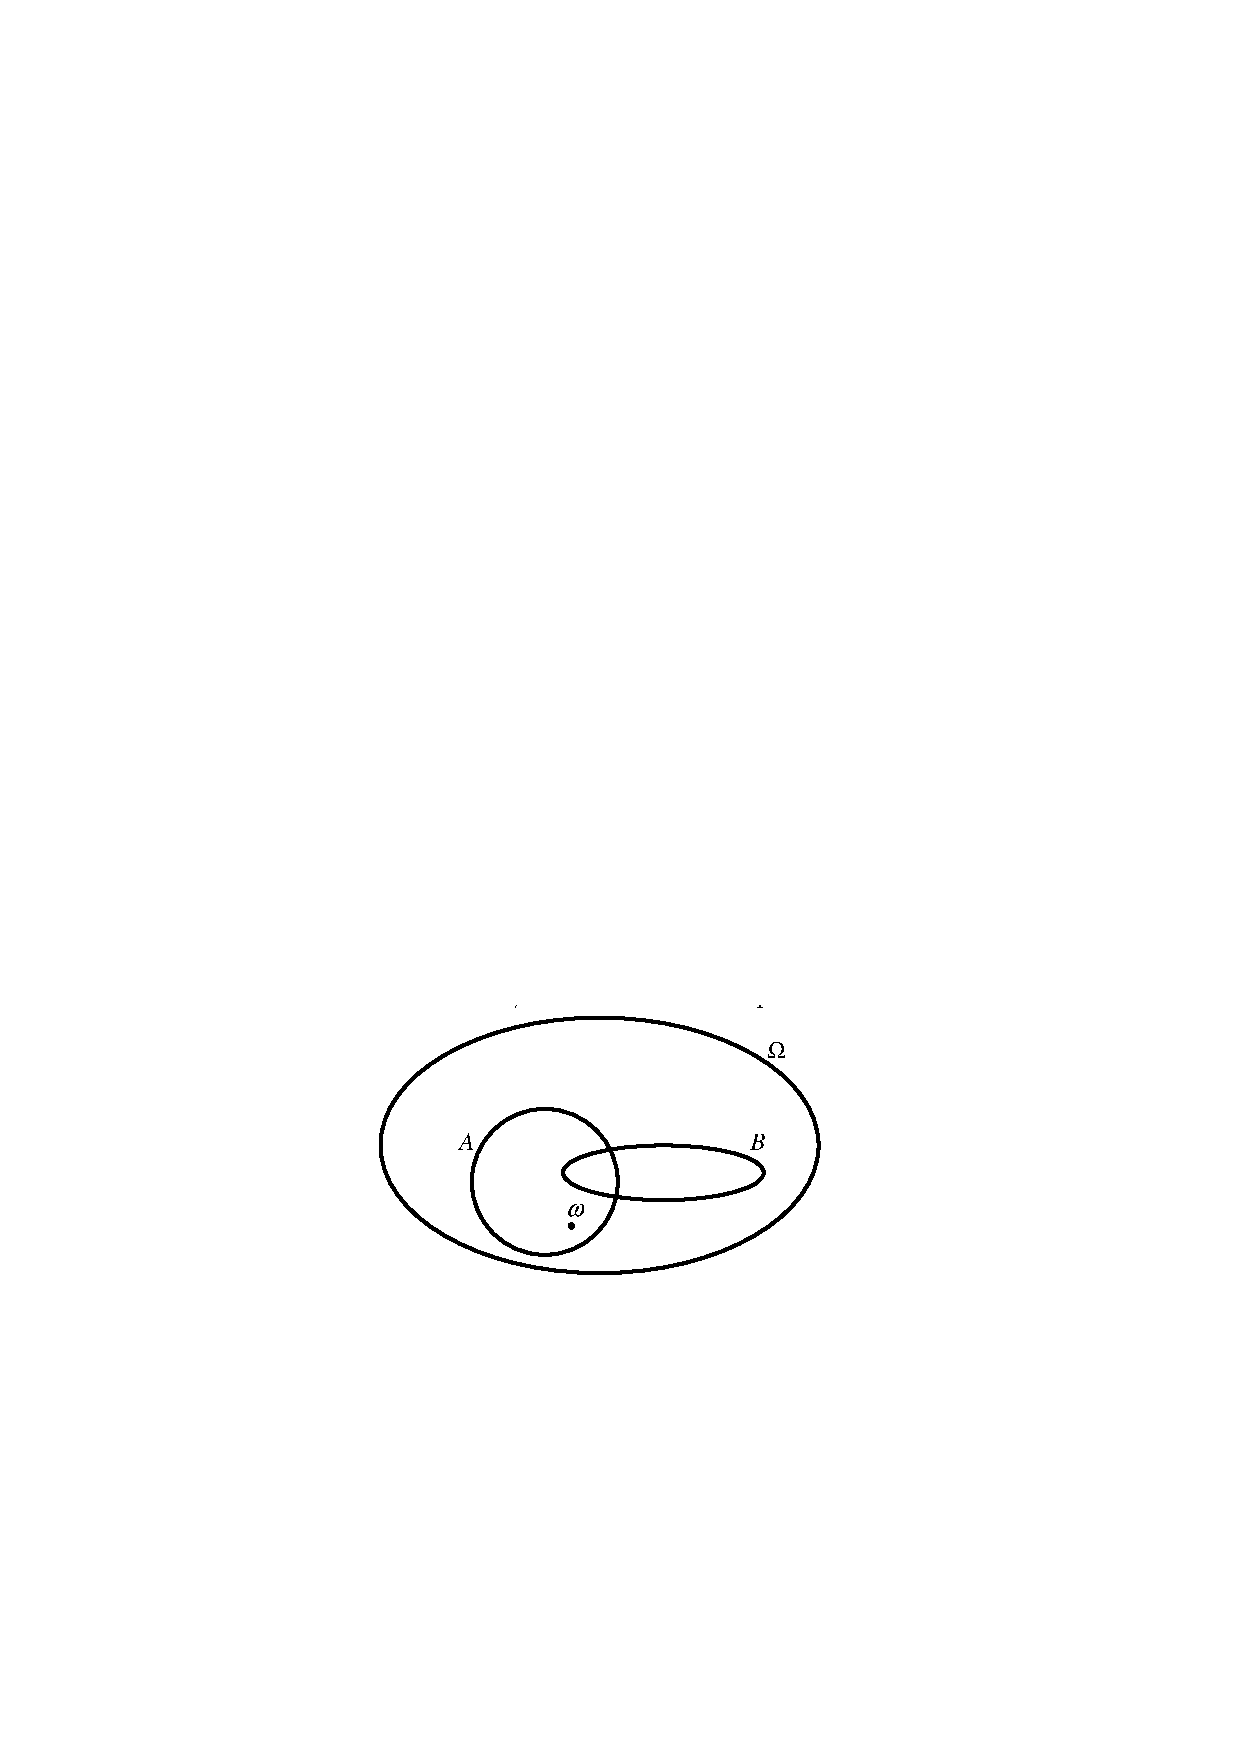
\includegraphics[]{pic/pic1}
	\caption{События в достоверном событии $\Omega$}
	\label{fig1}
\end{figure}

\begin{definition}
	\label{def:2.6}
1) Событие $A \cup B$ называется \textit{объединением} событий и состоит в том, что произошло хотя бы одно из событий $A$ или B.

2) Событие $A\cap B$ называется \textit{пересечением} событий $A$ и $B$ и состоит в
том, что произошли оба события $A$ и B.

3) Событие $A\backslash B$ называется \textit{разностью} событий $A$ и $B$ и состоит в том,
что событие $A$ произошло, а $B$ -- нет.

4) Событие $\overline{A}=\Omega\backslash A$ называется \textit{противоположным событию} $A$ и состоит в том, что событие $A$ не произошло. Ясно, что $A$ = $A$ (событие, противоположное к противоположному, является исходным событием).
Т.к. $\overline{\noo}=\Omega\backslash\noo$ и $\overline{\Omega}=\Omega\backslash\Omega=\noo$, то невозможное событие $\noo$ и
достоверное событие $\Omega$ являются взаимно противоположными (друг другу).

5) Говорят, что событие $A$ \textit{влечёт} событие $B$, и пишут $A\subset B$, если при
наступлении события $A$ происходит и событие $B$.
\end{definition}


\begin{definition}
	\label{def:2.7}
1) События $A$ и $B$ называются \textit{несовместными}, если
$A\cup B$ является невозможным событием, т.е. $A\cup B$ = $\noo$.

2) События $A_1,\cdots,A_n$ называются \textit{попарно несовместными}, если для любых $1\leq i<j\leq n$ события $A_i$ и $A_j$ несовместны.
\end{definition}

\begin{definition}
	\label{def:2.8}
Рассмотрим множество $\mathfrak{A}$, элементами которого являются события пространства $\Omega$ (не обязательно все!). Множество $A$ называется алгеброй событий, если достоверное событие $\Omega$ и любые события $A, B \in A$
удовлетворяют аксиомам:

Акс. $\mathcal{A}1$.$\quad$ $\Omega\in\mathfrak{A}$.

Акс. $\mathcal{A}2$.$\quad$ $A\cup B\in\mathfrak{A}$.

Акс. $\mathcal{A}3$.$\quad$ $A\cap B\in\mathfrak{A}$.

Акс. $\mathcal{A}4$.$\quad$ $A\backslash B\in\mathfrak{A}$.


Из аксиомы $\mathcal{A}1$ следует, что алгебра событий не может быть пустой; она всегда содержит достоверное событие $\Omega$. А т.к. $\Omega \backslash \Omega$ = $\noo$, то из аксиомы $\mathcal{A}4$ следует, что $\noo\in\mathfrak{A}$, т.е. любая алгебра событий $\mathfrak{A}$ содержит вместе с достоверным и невозможное событие.
\end{definition}

\textbf{Примеры}

1) Для любого пространства элементарных событий $\Omega$ набор из двух множеств $\mathfrak{A}_0=\{\noo,\Omega\}$ удовлетворяет аксиомам $\mathcal{A}1$--$\mathcal{A}4$, поэтому $\mathfrak{A}_0=\{\noo,\Omega\}$ является алгеброй событий. Алгебра событий $A_0$ называется тривиальной. Это самая маленькая алгебра событий.

2) В этом примере эксперимент -- подбрасывание игральной кости. 
Пространство элементарных событий есть $\Omega = \{1, 2, 3, 4, 5, 6\}$. 
Пусть событие $A = \{1, 3, 5\}$ -- выпадение нечётного числа очков, а событие $B= \{2, 4, 6\}$ -- выпадение чётного числа очков. 
Множество событий $\mathfrak{A}_1 = \{\noo, \Omega, A, B\}$ удовлетворяет аксиомам $\mathcal{A}1$--$\mathcal{A}4$, поэтому является алгеброй событий.

3) Для любого пространства элементарных событий $\Omega$ множество $\mathfrak{B}(\Omega)$ = множество всех подмножеств $\Omega$ удовлетворяет аксиомам $\mathcal{A}1$--$\mathcal{A}4$, поэтому является алгеброй событий. 
Эта алгебра событий является самой большой на $\Omega$. Для $\Omega= \{1, 2, 3, 4, 5, 6\}$ эта алгебра событий содержит 64 события.

4) Задайте ещё какую-нибудь алгебру событий на $\Omega = \{1, 2, 3, 4, 5, 6\}$.
Сколько различных алгебр событий можно задать на этом пространстве элементарных событий?

\begin{zam}
	\label{zam:2.9}
Из аксиом $\mathcal{A}1$--$\mathcal{A}4$ следует, что если к конечному набору событий из любой алгебры событий применить операции объединения, пересечения и вычитания конечное число раз, то полученное событие тоже содержится в этой алгебре.
\end{zam}

\begin{zam}
	\label{zam:2.10}
Если пространство элементарных событий конечно, $\Omega = \{\omega_1,\omega_2,\ldots,\omega_n\}$, то любая его алгебра событий тоже конечна. 
Это следует из того, что множество $\mathfrak{B}(\Omega)$ всех возможных событий, содержащихся в $\Omega$, тоже конечно и содержит $2^n$ событий.
\end{zam}

\begin{definition}
	\label{def:2.11}
Алгебра событий $\mathfrak{A}$ называется $\sigma$-алгеброй, если для любого счётного набора событий $A_1,A_2,\cdots \in \mathfrak{A}$ выполнена пятая аксиома:

Акс. $\mathcal{A}5$.$\quad$ $\bigcup\limits_{n=1}^\infty A_n \in\mathfrak{A}$.
\end{definition}


\begin{zam}
Из аксиом $\mathcal{A}1$--$\mathcal{A}4$ не следует, что объединение несчётного количества событий является событием из $\sigma$-алгебры. 
Рассмотрение несчётных объединений событий приводит к построению т.н. неизмеримых событий, вероятность наступления которых не существует. 
Первый пример такого неизмеримого события построил Витали\footnote{Джузеппе Витали (Giuseppe Vitali, 26.08.1875 -- 29.02.1932, Italy) -- итальянский математик.}. 
При построении неизмеримого множества Витали используется аксиома теории множеств -- аксиома выбора.
\end{zam}

\textbf{Аксиома выбора.} \textit{Для любого произвольного набора непустых непересекающихся множеств можно составить множество, выбрав в него по одному элементу из каждого множества этого набора.}

\begin{theorem}[Теорема Витали -- построение неизмеримого множества]
\textit{Существуют множества, длина которых не может быть выражена никаким числом.}
\end{theorem}

\begin{proof}
Для доказательства нам понадобятся лишь следующие очевидные свойства длины:

	\begin{itemize}
	\item длина дуги остается неизменной при повороте окружности вокруг
	центра;
	\item длина дуги, которая представляет собой объединение счетного количества попарно непересекающихся дуг, равна сумме длин этих
	дуг.	
	\end{itemize}	

Рассмотрим стандартную (единичного радиуса) окружность $S^1$. Она эквивалентна отрезку $[0, 2\pi)$, т.е. её длина равна $2\pi$. На этой окружности центральный угол в радианах равен длине дуги на которую он опирается.

Для любого рационального числа $\frac{p}{q}$ , где $q\ne 0$, рассмотрим дугу длины $\frac{2\pi p}{q}$.

Если отложить её на окружности $S^1$ последовательно $q$ раз, то полученная дуга замкнётся, т.е. начало 1-ой дуги совпадёт с концом $q$-ой.

Для любого иррационального числа $\alpha$ рассмотрим дугу длины $2\pi\alpha$. Ясно, что если отложить эту дугу $n$ раз на окружности $S^1$, то начало и конец дуги $2\pi\alpha n$ не совпадут ни при каком целом n. Это означает, что множество
\begin{equation*}
	A_0 = \{\ldots, -2\pi\alpha n, \ldots , -4\pi\alpha, -2\pi\alpha, 0, 2\pi\alpha, 4\pi\alpha, \ldots , 2\pi\alpha n, \ldots\}
\end{equation*}

является счётным. Заметим, что для любого целого $n$ поворот на угол $2\pi\alpha n$ переводит множество $A_0$ в себя.
Если взять произвольную точку (угол) $\phi \in [0, 2\pi)$ на окружности, такую чтобы $\phi \notin A_0$ , то множество
\begin{equation*}
	A_\phi = \{\ldots , \phi - 2\pi\alpha n, \ldots , \phi - 4\pi\alpha, \phi - 2\pi\alpha, \phi, \phi + 2\pi\alpha, \phi + 4\pi\alpha, \ldots , \phi + 2\pi\alpha n, \ldots \}
\end{equation*}

тоже является счётным, и для любого целого $n$ поворот множества $A_\phi$ на угол $2\pi n\alpha$ тоже переводит его в себя. 

Заметим, что т.к. $\phi \notin A_0$ , то множества $A_0$
и $A_\phi$ не пересекаются: если бы они имели общую точку, то при $n=\pm1, \pm2, \ldots$ все остальные их точки получились бы прибавлением дуг $2\pi\alpha n$, и тогда бы множества $A_0$ и $A_\phi$ совпадали. 

Заметим, что для любого целого $n$ поворот на
угол $2\pi\alpha n$ переводит множество $A_\phi$ в себя.

Если теперь выбрать угол $\psi \in [0, 2\pi)$, такой чтобы $\psi \notin A_0$ и $\psi \notin A_\phi$ , то множество
\begin{equation*}
	A_\psi = \{\ldots , \psi - 2\pi\alpha n, \ldots , \psi - 4\pi\alpha, \psi - 2\pi\alpha, \psi, \psi + 2\pi\alpha, \psi + 4\pi\alpha, \ldots , \psi + 2\pi\alpha n, \ldots \}
\end{equation*}

тоже является счётным, и для любого целого $n$ поворот множества $A_\psi$ на угол $2\pi\alpha n$ тоже переводит его в себя. Заметим, что т.к. $\psi \notin A_0$ и $\psi \notin A_\phi$, то
множество $A_\psi$ не пересекается ни с $A_0$ и ни с $A_\phi$. 

Заметим, что для любого целого $n$ поворот на угол $2\pi\alpha n$ переводит множество $A_\psi$ в себя.

Процесс построения таких непересекающихся множеств можно продолжить неограниченно
\footnote{
	В математике различают два типа бесконечности: потенциальная и актуальная бесконечности.

	Потенциальная бесконечность означает, что процесс построения какого-либо объекта может быть продолжен неограниченно. В нашем случае процесс построения множеств $A_\phi , A_\xi , A_\psi , \ldots$ может быть продолжен неограниченно (если не принимать во внимание, какое время может быть потрачено на это построение).
	Другой пример потенциальной бесконечности возникает при построении натурального ряда.
	Если мы выпишем все натуральные числа от 1 до $n$, то ничто не мешает нам написать число $n+1$, и т.д.
	Потенциальная бесконечность есть бесконечный процесс построения объектов, у которого нет последнего шага. Например, в доказательстве по методу математической индукции.

	Под актуальной бесконечностью понимается бесконечная совокупность, построение которой завершено, и все ее элементы наличествуют одновременно. Например, мы будем иметь дело с актуальной бесконечностью, если перечислим весь натуральный ряд полностью и имеем его в законченном виде
	$N = \{1, 2, \ldots , n, \ldots \}$. Актуальная бесконечность представляет собой весьма сильную идеализацию. В
	самом деле, она допускает не только возможность построения последующего объекта, если построен
	предыдущий, но и постулирует, что все возможные объекты уже построены и существуют одновременно.
	В нашем случае актуальная бесконечность означает, что процесс построения множеств $A_0, A_\phi, A_\psi , \ldots$
	закончен, и мы имеем это множество множеств $\{A_0, A_\phi, A_\psi , \ldots\}$ налицо.
}, пока не будут исчерпаны (выбраны) все точки окружности $S^1$ . В каждом таком множестве содержится счетное число точек, и все точки в одном множестве получаются друг из друга поворотами на угол $2\pi\alpha$.

Разные множества не пересекаются. Таким образом, окружность $S^1$ является объединением непересекающихся множеств $A_0, A_\phi, A_\psi , \ldots $ т.е.
\begin{equation*}
	S^1=\bigcup\limits_{\lambda\in\{0,\phi,\psi,\ldots\}}A_\lambda
\end{equation*}

Объединение счётного набора счётных множеств есть счётное множество.
А т.к. окружность $S^1$ состоит из несчетного множества точек, то набор построенных множеств $A_0, A_\phi, A_\psi , \ldots $ является несчётным. Другими словами множество индексов $\{0, \phi, \psi, \ldots ,\}$ -- несчётное.

Выберем из каждого множества $A_0, A_\phi, A_\psi , \ldots $ ровно по одной точке и по аксиоме выбора составим из этих точек множество $B_0$. 

Построенное множество $B_0$ называется \textit{множеством Витали}. Для каждого $n=\pm1, \pm2, \ldots$ обозначим через $B_n$ множество, которое получается в результате поворота множества $B_0$ на угол $2\pi n\alpha$. 

Ясно, что все множества $B_n$ , $n\in \mathbb{Z}$, имеют одну и ту же длину. Т.к. все точки множества $A_\lambda$ , где $\lambda \in \{0, \phi, \psi, \ldots\}$, можно получить, поворачивая одну из них на углы $2\pi n\alpha$, и т.к. в множестве $B_0$ собраны по одной точке из каждого множества $A_\lambda$ , то объединение всех $B_n$ составляет окружность $S^1$ , т.е.
\begin{equation*}
	S^1=\bigcup\limits_{n=-\infty}^{\infty}B_n
\end{equation*}

Оставшуюся часть доказательства проведём методом от противного. Предположим, что длина множества Витали $B_0$ существует, и обозначим её через $\mu(B_0)$. Тогда все множества $B_n$ имеют одну и ту же длину, т.к. получены из $B_0$ поворотом на угол кратный $2\pi\alpha$. Т.к. множества $B_n$ не пересекаются, то сумма их длин равна длине окружности $S^1$ . Поэтому

\begin{gather*}
	2\pi=\mu(S^1)=\mu\left(\bigcup\limits_{n=-\infty}^{\infty}B_n\right)=\sum\limits_{n=-\infty}^{\infty}\mu(B_n)=
	\sum\limits_{n=-\infty}^{\infty}\mu(B_0)=\\
	=
	\left\{
		\begin{aligned}
			\infty, \text{если } \mu(B_0)>0\\
			0, \text{если } \mu(B_0)=0
		\end{aligned}
	\right.
\end{gather*}

Полученное противоречие означает, что длины у множества Витали $B_0$ нет вообще никакой (ни нулевой, ни конечной, ни бесконечной). Такие множества и соответствующие им события называются \textit{неизмеримыми}.
\end{proof}

\begin{zam}
1) В предыдущем примере было доказано существование неизмеримого множества (множества Витали) и предъявлена конструкция его построения. Меняя иррациональное число $\alpha$, можно получить несчётное количество неизмеримых множеств на окружности $S^1 = [0, 2\pi)$. 

Если аксиому выбора не признавать, то неизвестно можно ли вообще построить неизмеримые множества. Можно доказать, что аксиома $\mathcal{A}5$ не допускает появление неизмеримых событий.

2) Если $\Omega$ -- несчётное множество (отрезок, площадка, объёмное тело), то множество P($\Omega$) всех подмножеств множества $\Omega$ не является $\sigma$-алгеброй, потому что оно содержит неизмеримые события.
\end{zam}

\begin{zam}
Все конечные и счётные алгебры событий являются $\sigma$-алгебрами.
\end{zam}

\begin{lemma}\label{lemmde}
Если ${A_1 , A_2 , \ldots }$ есть счётный набор событий из $\sigma$-алгебры $A$, то $\bigcap\limits_{n=1}^\infty A_n\in\mathfrak{A}$
\end{lemma}

\begin{proof}
Пусть $A1 , A2 , \ldots \in \mathfrak{A}$, Тогда из аксиомы $\mathcal{A}4$ следует, что
	\begin{equation*}
		\overline{A}_1,\overline{A}_2, \ldots \in \mathfrak{A},
	\end{equation*}
а из аксиомы $\mathcal{A}5$ следует, что
	\begin{equation*}
		\bigcup\limits_{n=1}^\infty \overline{A}_n\in\mathfrak{A}.
	\end{equation*} 
Тогда по аксиоме 4 дополнение к этому множеству тоже принадлежит $\mathfrak{A}$, т.е. 
	\begin{equation*}
		\overline{\bigcup\limits_{n=1}^\infty \overline{A}_n}\in\mathfrak{A}
	\end{equation*}
по формулам двойственности де Моргана
	\begin{equation*}
		\overline{\bigcup\limits_{n=1}^\infty \overline{A}_n}=\bigcap\limits_{n=1}^\infty {A}_n,
	\end{equation*} 
поэтому
	\begin{equation*}
		\bigcap\limits_{n=1}^\infty {A}_n\in\mathfrak{A}
	\end{equation*}

\end{proof}

\begin{consq}
	Лемма \ref{lemmde} и аксиома $\mathcal{A}5$ эквивалентны.
\end{consq}%Федя

\section{Вероятность и её свойства} 
%!TEX root = ../var.tex

\begin{definition}
	\label{def:3.1}
	Пусть $\Omega$ — пространство элементарных событий, и
$\mathfrak{A}$ — его $\sigma$-алгебра событий. Вероятностью называется функция множества
$\P: \mathfrak{A}\rightarrow \mathbb{R}$, удовлетворяющая следующим аксиомам:

Акс. $\mathcal{P}1$ (\textit{неотрицательность вероятности}). Для любого события $A\in\mathfrak{A}$ выполнено равенство $\P(A)\geqslant 0$.

Акс. $\mathcal{P}2$ (\textit{нормированность вероятности}). $\P(\Omega)=1$ 

Акс. $\mathcal{P}3$ (\textit{счётная аддитивность вероятности как функции множества}).
\end{definition}
Для любого счётного набора попарно несовместных событий \newline $A_1,A_2,\dots\in 
\mathfrak{A}$
имеет место равенство
\begin{equation*}
	\P\left(\bigcup_{n=1}^{\infty}A_n \right)=\sum^{\infty}_{n=1}\P(A_n) \notag
\end{equation*}
В частности, эта аксиома справедлива и для конечного набора попарно несов
местных событий.
Акс. $\mathcal{P}1$ (непрерывность вероятности). Для любой убывающей последовательности событий $A_1 \supset A_2 \supset\dots\supset A_n \supset \dots$ из $\sigma$-алгебры $\mathfrak{A}$ такой, что $\bigcap_{n=1}^{\infty}A_n=\noo$,
выполняется равенство
\begin{equation*}
	\lim\limits_{n\to\infty}\P(A_n)=0 \notag
\end{equation*}
\begin{definition}
	\label{def:3.2}
	Тройка $(\Omega,\mathfrak(A),\P)$ называется \textit{вероятностным пространством}.
\end{definition}
Докажем теперь основные свойства вероятности пп. \ref{lemma:3.3} – \ref{th:3.12}.

\begin{figure}[h!]
	\centering
	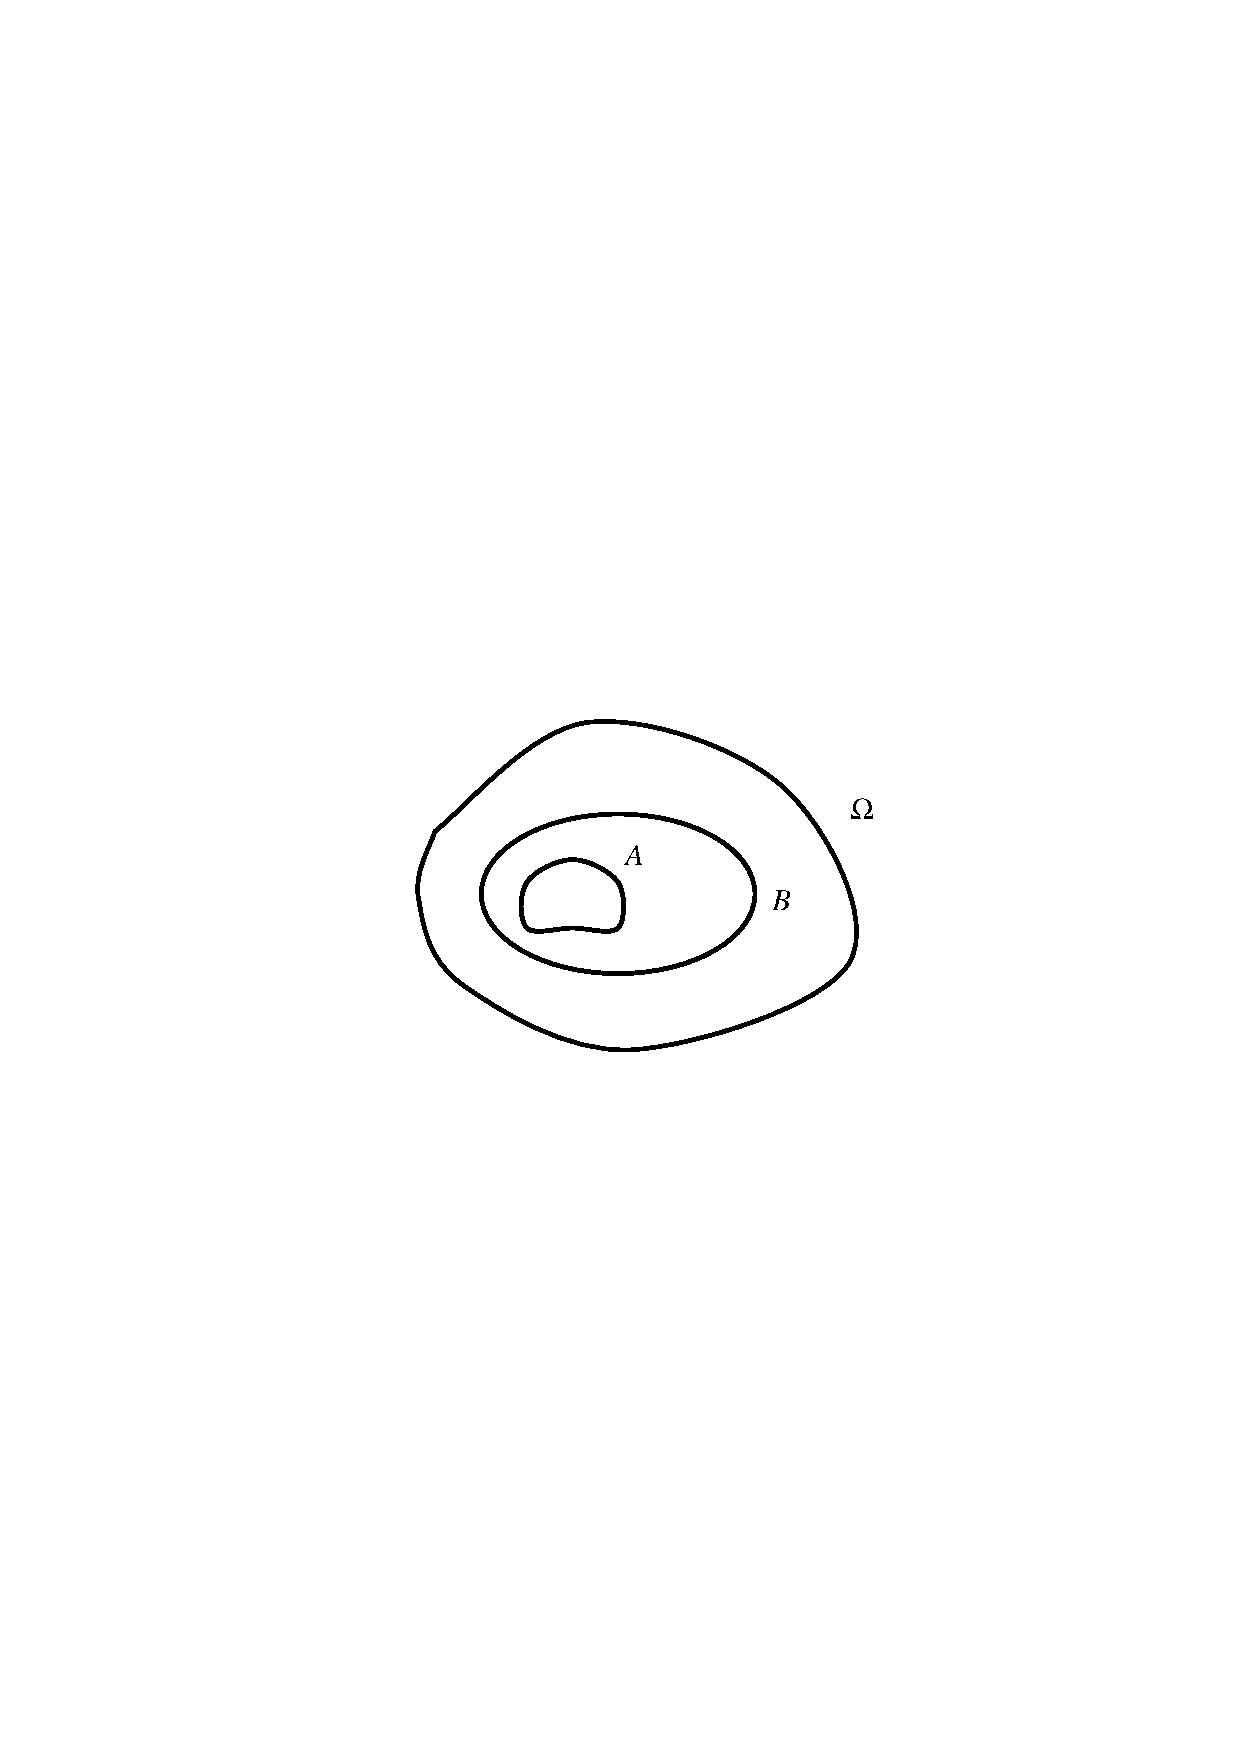
\includegraphics[width=0.5\textwidth]{pic/pic2.pdf}
	\caption{Если $A\subseteq B$, то $\P(B\ssm A=\P(B)-\P(A))$.}
	\label{fig2}
\end{figure}
\begin{lemma}
	\label{lemma:3.3}
	Если событие A влечёт событие B, т.е $A\subseteq B$, то $\P(B\ssm A)=\P(B)-\P(A)$ (см. рис. \ref{fig2})
\end{lemma}

\begin{proof}
	Т.к. $B=A\cup(B\ssm A)$,  и события A и $B\ssm A $ несовместны, то по аксиоме $\mathfrak{\P}$ имеем $\P(B)=\P(A)+\P(B\ssm A)$, что и требовалось доказать.
\end{proof}


\begin{consq}
	\label{consq:3.4}
	Если $A\subseteq B$, то $\P(A)\geqslant \P(B)$. 
\end{consq}

\begin{lemma}
	\label{lemma:3.5}
	$\P(\noo)=0$.
\end{lemma}
\begin{proof}
	$\P(\noo)=\P(\Omega\ssm\Omega)=\P(\Omega)=\P(\Omega)=1-1=0$
\end{proof}

\begin{lemma}
	\label{lemma:3.6}
	Для любого события $A\in\mathfrak{A}$ выполнено неравенство
	\begin{equation*}
		0\leqslant \P(A)\leqslant 1
	\end{equation*}
\end{lemma}
\begin{proof}
	Т.к. $\O\subseteq A\subseteq\Omega$, то из след. \ref{consq:3.4} следует утверждение леммы. 
\end{proof}

\begin{lemma}
	\label{lemma:3.7}
	Для любого события $A\in\mathfrak(A)$ имеем $\P(\bar{A})=1-\P(A)$
\end{lemma}

\begin{proof}
	$\P(\bar{A})=\P(\Omega\ssm A)=\P(\Omega-\P(A)=1-\P(A)$
\end{proof}

\begin{lemma}
	\label{lemma:3.8}
	Для любых событий $A,B\in\mathfrak(A)$ выполнено равенство 
\begin{equation*}
	\P(A\cup B)=\P(A)+\P(B)-\P(A\cap B).
\end{equation*}
	
\end{lemma}
\begin{proof}
	Т.к. $A\cup B = A \cup(B \ssm (A \cup B))$, и события $A$ и
$B \ssm (A \cup B)$ несовместны, то применяя сначала Акс. $\mathcal{P}3$, а затем лемму \ref{lemma:3.3}
получим $\P(A\cup B) = \P(A) + \P(B \ssm (A\cup B)) = \P(A) + \P(B) − \P(A \cup B)$.
\end{proof}
\begin{consq}
	\label{consq:3.9}
	Для любых событий $A,B\in\mathfrak{A}$ выполнено равенство 
	\begin{equation*}
		\P(A\cup B)\geqslant \P(A)+\P(B).
	\end{equation*}
\end{consq}

\begin{consq}
	\label{consq:3.10}
	Если события A и B несовместны, т.е $A\cap B=\O$, то 
\begin{equation*}
		\P(A\cup B)\leqslant \P(A)+\P(B).
\end{equation*}
\end{consq}

\begin{proof}
	По лемме \ref{lemma:3.8} имеем $\P(A\cup B)=\P(A)+\P(B)-\P(A\cap B)=\P(A)+\P(B)-\P(\noo)=\P(A)+\P(B)$.
\end{proof}

\begin{consq}
	\label{consq:3.11}
	$\P(A_1\cup\dots\cup A_n)\leqslant\sum\limits^n_{i=1}\P(A_i)$.
\end{consq}	
\begin{theorem}
\label{th:3.12}
\begin{gather*}
	\P(A_1\cup A_2\cup\dots A_n)
	=\sum\limits_{i=1}^n \P(A_i)
	-\sum\limits_{1\leqslant i<j	\leqslant n} \P(A_i\cap A_j)\\
	+ \sum\limits_{1\leqslant i<j<m\leqslant n}\P(A_i\cap A_j \cap A_m)-
	\dots
	+(-1)^{n-1}\P(A_1\cap A_2\cap\dots\cap A_n).
\end{gather*}
\begin{proof}
	Применяя метод математической индукции и лемму \ref{lemma:3.8}
получим требуемый результат.
\end{proof}
\end{theorem}
%Кирилл

\section{Способы задания и подсчёта вероятности}
%!TEX root = ../var.tex

\subsection{Экспериментальное нахождение вероятности}

В этом пункте описан способ экспериментального определения вероятности
наступления так называемых массовых событий.

\begin{definition}
  	Событие A называется \textit{массовым}, если опыт (эксперимент, испытание), при котором событие A может произойти, можно повторить \textit{неограниченное число раз при одних и тех же условиях}.
\end{definition} 

Методами теории вероятностей изучают (в основном) эксперименты, которые порождают массовые события. Всюду до конца лекций будут рассматриваться только массовые события.

\begin{example}
1) Опыт: однократное подбрасывание ломаного гроша.
События выпадение орла $O$ и выпадение решки $P$ являются массовыми событиями. Заметим, что пространство элементарных событий 
$\Omega = \{O, P \}$ состоит из конечного числа элементарных исходов.

2) Опыт: подбрасывание ломаного гроша до появления первого орла. События $P , OP , OOP, \ldots, O \ldots OP , \ldots$ являются массовым. Заметим, что в этом примере пространство $\Omega=\{P, OP, OOP, \ldots, O \ldots OP, \ldots\}$ состоит из
счётного количества элементарных исходов: положение кольца однозначно определяется положением его центра.

3) Опыт: бросание обручального кольца на клетчатую скатерть (диаметр кольца меньше стороны клетки). Событие $A$: кольцо падает внутрь какой-нибудь клетки, не пересекая её границы. Это событие является массовым.
Заметим, что в этом примере пространство состоит из несчётного количества элементарных исходов.
 \end{example} 

Типичность этих трёх примеров состоит в том, что в теории вероятностей встречаются три типа пространств элементарных событий: конечные, счётные и несчётные.

\begin{definition}
	Если в результате n испытаний массовое событие $A$ произошло $\mu(A)$ раз, то число $\frac{\mu(A)}{n}$
называется \textit{относительной частотой} появления события $A$.
\end{definition}

Для каждого примера 4.2 можно провести $n$ опытов, сосчитать число $\mu(A)$ появлений этого события и подсчитать относительную частоту $\frac{\mu(A)}{n}$.

Массовые события обладают свойством <<статистической устойчивости>>, а именно: \textit{при увеличении числа экспериментов относительная частота $\frac{\mu(A)}{n}$
появления события $A$ имеет тенденцию стабилизироваться, стремясь к некоторому числу $P(A)$.}
\begin{definition}
Число $P(A) = \lim\limits_{n\to\infty} \frac{\mu(A)}{n}$ называется \textit{статистической вероятностью} события $A$ и находится при больших $n$ по приближённой формуле $P(A)\approx \mu(A)$.
\end{definition} 

\subsection{Вероятность на конечном пространстве.}
Пусть задано конечное пространство $\Omega=\{\omega_1,\omega_2,\ldots,\omega_n\}$, состоящее из $n$ элементарных событий (исходов), и заданы вероятности наступления этих
событий $P(\omega_1 ) = p_1 , P(\omega_2 ) = p_2 , \ldots , P(\omega_n ) = p_n$ так, что $p_1 + p_2 + \ldots + p_n = 1$.
Обозначим через $\omega$ переменную величину, принимающую значения из $\Omega$.

\begin{definition}
Такое соответствие записывается в виде таблицы
\begin{center}
	\begin{tabular}{|l|l|l|l|l|}
		\hline
		$\omega$ & $\omega_1$ & $\omega_2$ & $\ldots$ & $\omega_n$ \\ \hline
		$P(\xi)$  & $p_1$ & $p_2$ & $\ldots$  & $p_n$ \\ \hline
	\end{tabular}
\end{center}


которая называется \textit{рядом распределения} случайных исходов или \textit{законом
распределения}. Если $n = 2$, то ряд называется \textit{схемой Бернулли}. Если $n \geq 3$,
то ряд называется \textit{схемой независимых испытаний с несколькими исходами}.
\end{definition}

Ряд распределения задаёт функцию в виде таблицы, которая каждому элементарному исходу ставит в соответствие вероятность его наступления.

Потребуем теперь выполнение аксиомы $\mathcal{P}3$.

\begin{deflemma}[Формула вероятности на конечном пространстве]

Если  вероятность, определяемая рядом распределения из опред. 4.5, подчиняется аксиоме $\mathcal{P}3$, то вероятность события $A = \{\omega_{i_1} , \omega_{i_2} , \ldots ,  \omega_{i_k} \} \subset \Omega$ вычисляется по формуле
%
$$P(A) = p_{i_1} + p_{i_2} + \ldots + p_{i_k} ,$$

которая называется формулой вероятности на конечном пространстве.
\end{deflemma}
\begin{proof}
\begin{gather*}
 	P(A) = P (\omega_{i_1} , \omega_{i_2} , \ldots , \omega_{i_k}) =\\= P \left( \bigcup\limits_{j=1}^k \{\omega_{i_j} \} \right) \stackrel{\mathcal{P}3}{=} \sum_{j=1}^{k} P(\omega_{i_j}) = \sum_{j=1}^{k} p_{i_j} = p_{i_1} + p_{i_2} + \ldots + p_{i_k}.
\end{gather*}
\end{proof} 
\begin{example}
Простейший ряд распределения имеет эксперимент с детерминированным исходом, $\Omega = \{ \omega \}$ (см. опред. \ref{def:2.3}):
\begin{center}
	\begin{tabular}{|l|l|}
		\hline
		$\xi$ & $\omega$  \\ \hline
		$P$  & $1$  \\ \hline
	\end{tabular}
\end{center}
Этот тривиальный случай удовлетворяет всем аксиомам и определениям, однако никакого значения в теории вероятностей не имеет. Придётся с этим
мириться.
\end{example}
\begin{definition}
	Пусть в результате опыта могут возникнуть только
два события: <<успех>>, который обозначается единицей — 1 и наступает c вероятностью $p$, и <<неудача>>, которая обозначается нулём — 0 и наступает c
вероятностью $q = 1−p$; $\Omega = \{0, 1\}$. Такой опыт называется \textit{схемой Бернулли}\footnote{
	Якоб Бернулли (Jakob Bernoulli, 1654-1705), швейцарский математик
}
и имеет ряд распределения

\begin{center}
	\begin{tabular}{|c|c|c|}
		\hline
		$\xi$ & 0 & 1  \\ \hline
		$P$  & $q=1-p$ & p \\ \hline
	\end{tabular}
\end{center}

\end{definition}

Схема Бернулли является первым нетривиальным примером вероятности на конечном пространстве.

Схема Бернулли имеет простую интерпретацию. Рассмотрим ломаный грош с вероятностями выпадения орла $p$ и решки $q = 1 − p$. Обозначим появление орла через 1, а его не выпадение через 0, получим схему Бернулли.

\begin{example}[Геометрическая интерпретация схемы независимых  испытаний с несколькими исходами.]
Рассмотрим произвольный выпуклый многогранника с $n$ гранями, на которых написаны символы $\omega_1 , \omega_2 , \ldots , \omega_n$.

При этом многогранник должен быть таким, чтобы перпендикуляр, опущенный из его центра тяжести на любую грань, пересекал эту грань в её внутренней точке (чтобы многогранник, падая на эту грань, не перекатывался на другую).

Пусть вероятности выпадения многогранника гранью вниз равны соответственно $p_1 , p_2 , \ldots , p_n$ , где естественно $p_1 + p_2 + \ldots +p_n = 1$. 

Легко видеть, что вероятность $p_i$ пропорциональна телесному углу $\alpha_i$ с вершиной $C$ в центре тяжести многогранника, опирающегося на грань $\omega_i$.

Так как сумма всех телесных углов с вершиной $C$ равна $4\pi$ стерадиан, т.е. $\alpha_1 + \alpha_2 + \ldots + \alpha_n = 4\pi$, то
$$\frac{\alpha_1}{4\pi} + \frac{\alpha_2}{4\pi} + \ldots + \frac{\alpha_n}{4\pi}
 = 1,$$ поэтому $p_i = 4\pi$.
\end{example}

\subsection{Классическая вероятность}

Классическая вероятность является частным случаем вероятности на конечном пространстве, когда вероятность подчинена принципу равной вероятности. Исторически классическая вероятность применялась в теории азартных игр и появилась раньше вероятности на конечном пространстве.

\textbf{Принцип равной вероятности.} \textit{Если на конечном пространстве $\Omega$ вероятность наступления его элементарных исходов $\omega_1 , \omega_2 , \ldots , \omega_n$ одна и та же,
$$p_1 = p_2 = \ldots = p_n = p,$$
то говорят, что вероятность на конечном пространстве удовлетворяет
принципу равной вероятности (или равной возможности).}

Выпадение орла и решки при подбрасывании симметричной монеты; выпадение граней при подбрасывании правильного многогранника (тетраэдра, куба, октаэдра, додекаэдра или икосаэдра); появление к.-л. карты из полной
колоды карт удовлетворяют принципу равной возможности.

Классическая вероятность характеризуется только числом элементарных исходов $n$ в пространстве $\Omega$. Она имеет ряд распределения

\begin{center}
	\begin{tabular}{|c|c|c|c|c|}
		\hline
		$\omega$ & $\omega_1$ & $\omega_2$ & $\ldots$ & $\omega_n$ \\ \hline
		$P(\omega)$  & $p$ & $p$ & $\ldots$  & $p$ \\ \hline
	\end{tabular}
\end{center}

где $np = 1$, поэтому $p = \frac{1}{n}$.


\begin{lemma}[Формула классической вероятности]
Если вероятность $P$ удовлетворяет принципу равной возможности, то вероятность наступления события $A = \{ \omega_{i_1} , \omega_{i_2} , \ldots , \omega_{i_k} \} \subset \Omega$ определяется по формуле, называемой формулой классической вероятности,
$$P(A) = \frac{k}{n}$$
\end{lemma} 
\begin{proof}
	$P(A) = p_{i_1} + p_{i_2} + \ldots + p_{i_k} = kp = \frac{k}{n}$
\end{proof}

Если обозначить число $k$ элементов множества $A$ через $\mu(A)$, а число $n$ элементов пространства $\Omega$ через $\mu(\Omega)$, то формулу классической вероятности
можно записать в виде
$$P(A) = \frac{\mu(A)}{\mu(\Omega)}$$
Число $\mu(A) = k$ называется числом исходов, \textit{благоприятствующих} наступлению события $A$.

\begin{zam}

1) Вероятности элементарных исходов в экспериментах с шариками, описанные в теоремах \ref{th:1.4}, \ref{th:1.6} и \ref{th:1.7}, удовлетворяют принципу равной возможности. Эти вероятности соответственно $1/A_n^k , 1/C_n^k$ и $1/n^k$.

2) Вероятности элементарных исходов в теореме \ref{th:1.9} (выбор с возвращением и без учёта порядка) не удовлетворяют этому принципу. Например, при $n = 2$
и $k = 2$ вероятности элементарных событий имеют ряд распределения

\begin{center}
	\begin{tabular}{|c|c|c|c|}
		\hline
		$\omega$ & $(1,1)$ & $(1,2)$ & $(2,2)$ \\ \hline
		$P(\omega)$  & $1/4$ & $1/2$  & $1/4$ \\ \hline
	\end{tabular}
\end{center}

3) Следует отметить, что при рассмотрении подобных вопросов ошибались даже такие великие математики, как, например, Д'Аламбер. 

Так, однажды у Даламбера спросили, с какой вероятностью монета, брошенная дважды, хотя бы один раз выпадет гербом. Ответ учёного был $\frac{2}{3}$, т.к. он считал, что есть 3 возможных исхода (герб-герб, герб-решка, решка-решка) и среди них 2 благоприятствующих. 

Д'Аламбер пренебрегал тем, что эти три возможных исхода не равновозможны. 

Правильным ответом является $\frac{3}{4}$ , поскольку из четырёх равновозможных исходов (герб-герб, герб-решка, решкагерб, решка-решка) три благоприятствуют указанному событию. 

Точка зрения Д'Аламбера была даже опубликована во Французской энциклопедии в 1754 г. в статье <<Герб и решётка>> (<<Croix on pile>>).
\end{zam}
 

\subsection{Вероятность на счётном пространстве}
Пусть теперь $\Omega = \{\omega_1 , \omega_2 , \ldots , \omega_n , \ldots \}$ – счётное пространство. Пусть $p_1 + p_2 + \ldots + p_n + \ldots = 1$ — сходящийся (к единице) числовой ряд, удовлетворяющий
для всех $i \in \mathbb{N}$ условию $0 < p_i < 1$. Последнее условие позволяет трактовать члены этого ряда как вероятности элементарных событий пространства $\Omega$.

\begin{definition}
Вероятность элементарных исходов, заданная в виде таблицы
\begin{center}
	\begin{tabular}{|c|c|c|c|c|c|}
		\hline
		$\omega$ & $\omega_1$ & $\omega_2$ & $\ldots$ & $\omega_i$ & $\ldots$ \\ \hline
		$P(\omega)$  & $p_1$ & $p_2$ & $\ldots$  & $p_i$ & $\ldots$ \\ \hline
	\end{tabular}
\end{center}
называется \textit{рядом распределения на счётном пространстве}.
Потребуем теперь выполнение аксиомы $\mathcal{P}3$.
\end{definition}

\begin{lemma}[Формула вероятности на счётном пространстве]

Если события из пространства $\Omega$ подчиняются аксиоме $\mathcal{P}3$, то вероятность события $A = \{\omega_{i_1} , \omega_{i_2} , \ldots , \omega_{i_k} , \ldots \} \subset \Omega$ вычисляется по формуле
$$P (A) = p_{i_1} + p_{i_2} + \ldots + p_{i_k} + \ldots$$
\end{lemma}

\begin{proof}
\begin{gather*}
	P(A) = P(\omega_{i_1},\omega_{i_2}, \ldots, \omega_{i_k}, \ldots) =\\= P \left( \bigcup_{j=1}^\infty \{ \omega_{i_j}\} \right) \stackrel{\mathcal{P}3}{=} \sum_{j=1}^{\infty} P(\omega_{i_j}) = \sum_{j=1}^{\infty} p_{i_j} = p_{i_1} + p_{i_2} + \ldots + p_{i_k} + \ldots 
\end{gather*}
	
\end{proof}

\begin{zam}
Каждому степенному ряду на той части его интервала
сходимости, на которой его члены положительны, можно поставить в соответствие параметрическое семейство распределений со счётным пространством.
Рассмотрим, например, экспоненту $e^\lambda$ . Её ряд МакЛорена
$$1+ \frac{\lambda}{1!} + \frac{\lambda^2}{2!} + \ldots + \frac{\lambda^k}{k!} = e^\lambda$$
сходится при всех значениях $−\infty < \lambda < \infty$ и имеет положительные члены при $\lambda > 0$. Умножим обе части этого тождества на $e^{−\lambda}$ , получим тождество

$$e^{−\lambda}+ \frac{\lambda}{1!} e^{−\lambda} + \frac{\lambda^2}{2!} e^{−\lambda}+ \ldots + \frac{\lambda^k}{k!} e^{−\lambda}= 1$$

Составим следующий ряд распределения:

\begin{center}
	\begin{tabular}{|c|c|c|c|c|c|c|}
		\hline
		$k$ 			& 0 								& 1 				  & 2 & $\ldots$ & $k$ 		& $\ldots$ \\ \hline
		&&&&&& \\[-1em] 
		$P_\lambda(k)$  & $e^{-\lambda}$ & $\frac{\lambda}{1!}e^{-\lambda}$ & $\frac{\lambda^2}{2!}e^{-\lambda}$ & $\ldots$ & $\frac{\lambda^k}{k!}e^{-\lambda}$& $\ldots$ \\[1ex] \hline
	\end{tabular}
\end{center}
\end{zam}

\begin{definition}
Распределение, реализуемое этим рядом, называется \textit{распределением Пуассона с параметром $\lambda$.}

На рис. 25 показаны функции $P_\lambda (k)$ для для параметра $\lambda = 0, 1; 1; 10,$ где
пунктиром показаны огибающие. В каждом случае сумма длин вертикальных отрезков равна 1.

Распределение Пуассона описывает, например, вероятность $P_\lambda (k) = \frac{\lambda^k e^{-\lambda}}{k!}$
поступления на телефонную станцию $k$ звонков за какой-нибудь фиксированный промежуток времени, где число звонков $k = 0, 1, 2, \ldots$.
\end{definition}. 
\begin{zam}
Другим источником построения распределений со счётным пространством являются сходящиеся числовые ряды с положительными членами. Например, известно (Л. Эйлер), что
$$\frac{1}{1^2} + \frac{1}{2^2} + \frac{1}{3^2} + \ldots + \frac{1}{k^2} + \ldots = \frac{\pi^2}{6}.$$
Разделив обе части этого числового тождества на $\frac{\pi^2}{6}$ , можно получить (безымянный) ряд распределения, задаваемый формулой $P(k) = \frac{1}{k^2} \cdot \frac{6}{\pi^2}$ , со счётным пространством $\Omega = \mathbb{N}$.
Среди числовых рядов наиболее встречающимися в теории вероятностей являются геометрические прогрессии с положительными членами.
\end{zam}

\begin{definition}
Если члены ряда $p_1 + p_2 + \ldots + p_n + \ldots = 1$ положительны и являются членами убывающей геометрической прогрессией с первым членом $p_1 = p$ и с знаменателем $q = 1 − p$, то вероятность на счётном пространстве называется \textit{геометрическим распределением}. Геометрическое распределение имеет ряд
\begin{center}
	\begin{tabular}{|c|c|c|c|c|c|}
		\hline
		$\tau_1$ & $\omega_1$ & $\omega_2$ & $\ldots$ & $\omega_k$ & $\ldots$ \\ \hline
		$P$  & $q$ & $qp$ & $\ldots$  & $q^{k-1}p$& $\ldots$ \\ \hline
	\end{tabular}
\end{center}
\end{definition}

\begin{example}
Рассмотрим схему Бернулли (ломаного гроша) с вероятностью <<успеха>> (выпадения орла -- события 1) равной $p$. Она имеет ряд распределения

\begin{center}
	\begin{tabular}{|c|c|c|}
		\hline
		$\xi$ & 0 & 1  \\ \hline
		$P$  & $1-p$ & p \\ \hline
	\end{tabular}
\end{center}

Пусть эксперимент состоит в том, что испытания по схеме Бернулли проводятся неограниченное число раз. С таким экспериментом связаны две случайные величины: $\tau_1$ — номер первого выпавшего орла и $\tau_0$ — число выпавших решек, появившихся до первого орла. Легко подсчитать, что случайные величины $\tau_0$ и $\tau_1$ имеют ряды распределения

\begin{center}
	\begin{tabular}{|c|c|c|c|c|c|}
		\hline
		$\tau_0$ & $0$ & $1$ & $\ldots$ & $k$ & $\ldots$ \\ \hline
		$P$  & $q$ & $qp$ & $\ldots$  & $q^k p$& $\ldots$ \\ \hline
	\end{tabular}
	\quad и \quad
	\begin{tabular}{|c|c|c|c|c|c|}
		\hline
		$\tau_1$ & $1$ & $2$ & $\ldots$ & $k$ & $\ldots$ \\ \hline
		$P$  & $q$ & $qp$ & $\ldots$  & $q^{k-1} p$& $\ldots$ \\ \hline
	\end{tabular}
\end{center}

В строке вероятностей эти ряды содержат одну и ту же геометрическую
прогрессию; они называются соответственно $\tau_0$-- и $\tau_1$-- геометрическим распределениями. Эти случайные величины связаны очевидной формулой $\tau_1 = \tau_0 + 1$.

Формула вероятности для $\tau_0$ -- геометрического распределения определена по формуле
$$P(\tau_0 = k) = q^k p,$$
где $0 < p < 1$ и $q = p − 1$.
Формула вероятности для $\tau_1$ -- геометрического распределения:
$$P(\tau_1 = k) = q^{k−1} p,$$
где $0 < p < 1$ и $q = p − 1.$
\end{example}

\subsection{Геометрическая вероятность}

Рассмотрим ограниченную измеримую область $\Omega \subset \mathbb{R}^n$ , состоящую из несчётного множества точек. '

Измеримость области означает: на прямой область $\Omega \subset \mathcal{R}^1$ имеет конечную ненулевую длину, на плоскости область $\Omega \subset \mathcal{R}^2$ имеет конечную ненулевую площадь, в пространстве область $\Omega \subset \mathcal{R}^3$ имеет конечный ненулевой объём и т.д. 

Пусть на $\Omega$ определена $\sigma$-алгебра $\mathfrak{A}$. Для любого события $A \in \mathfrak{A}$ обозначим через $\mu(A)$ его меру (длину, площадь, объём и т.д. соответственно). 

Пусть эксперимент состоит в том, что в область $\Omega$ бросают точку.

\textbf{Принцип равномерности}\footnote{
Вероятности, которые не подчиняются этому принципу, являются главным предметом изучения теории вероятностей. Они будут изучены в гл. 2. <<Теория случайных величин>>.	
}. 
\textit{Если для любого события $A \in \mathfrak{A}$ его вероятность задаётся по формуле
$$P(A) = \alpha \mu(A),$$
где $\alpha$ — постоянное число, независящее от выбора события $A$ (т.е. не зависящее от формы $A$ и его расположения в $\Omega$), то говорят, что вероятность $P(A)$ удовлетворяет принципу равномерности.}

\begin{lemma}
Если вероятность $P(A)$ удовлетворяет принципу равномерности, то
$$\alpha=\frac{1}{\mu(\Omega)}$$
\end{lemma}

\begin{proof}
	Подставим в формулу $P(A) = \alpha \mu(A)$ достоверное событие $\Omega \in \mathfrak{A}$, получим: $1 = \alpha\mu(\Omega).$
\end{proof} 

\begin{definition}
Полученная формула
$$P(A) = \frac{\mu(A)}{\mu(\Omega)}$$
называется формулой \textit{геометрической} вероятности. (Не путать с геометрическим рядом распределения!)
\end{definition}

\begin{figure}[h!]
	\centering
	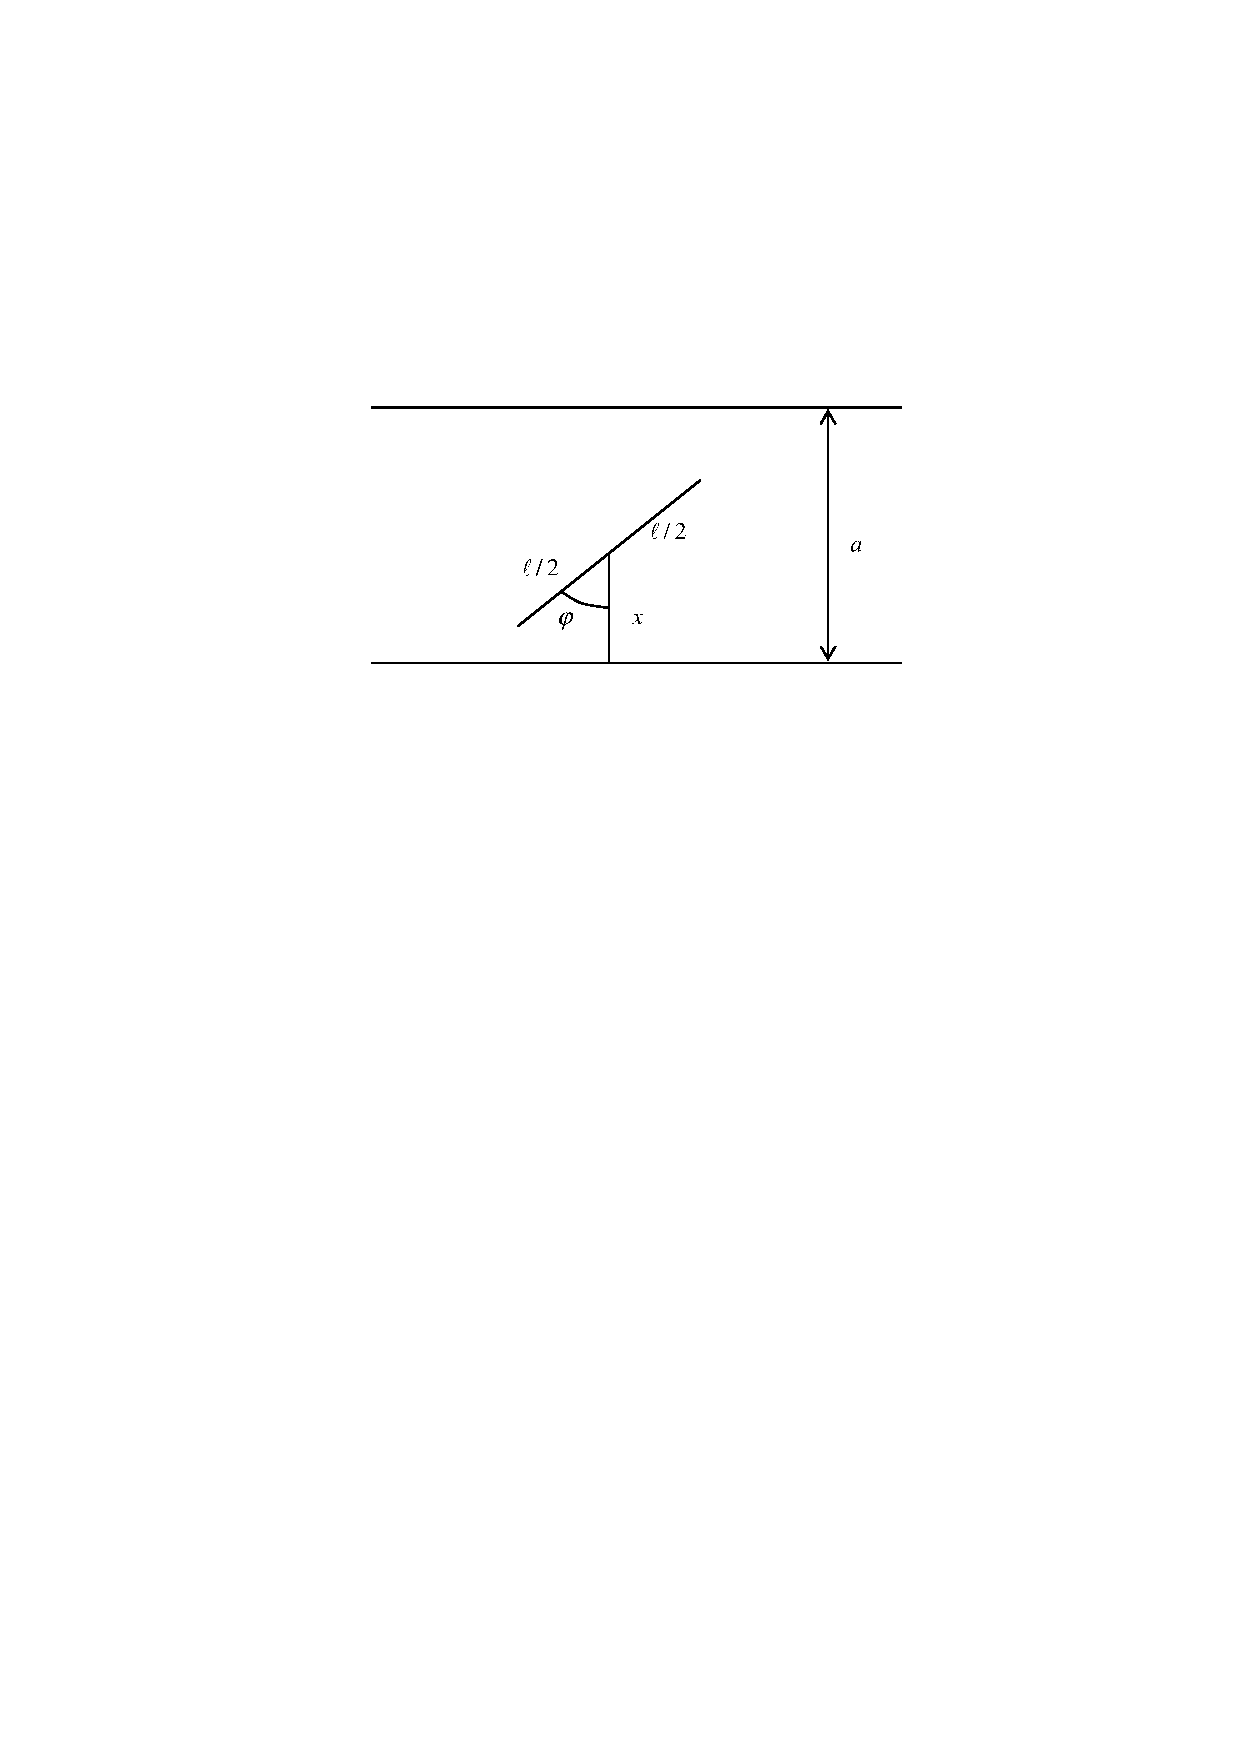
\includegraphics[]{pic/pic3}
	\caption{Задача Бюффона}
	\label{fig3}
\end{figure}
\begin{figure}[h!]
	\centering
	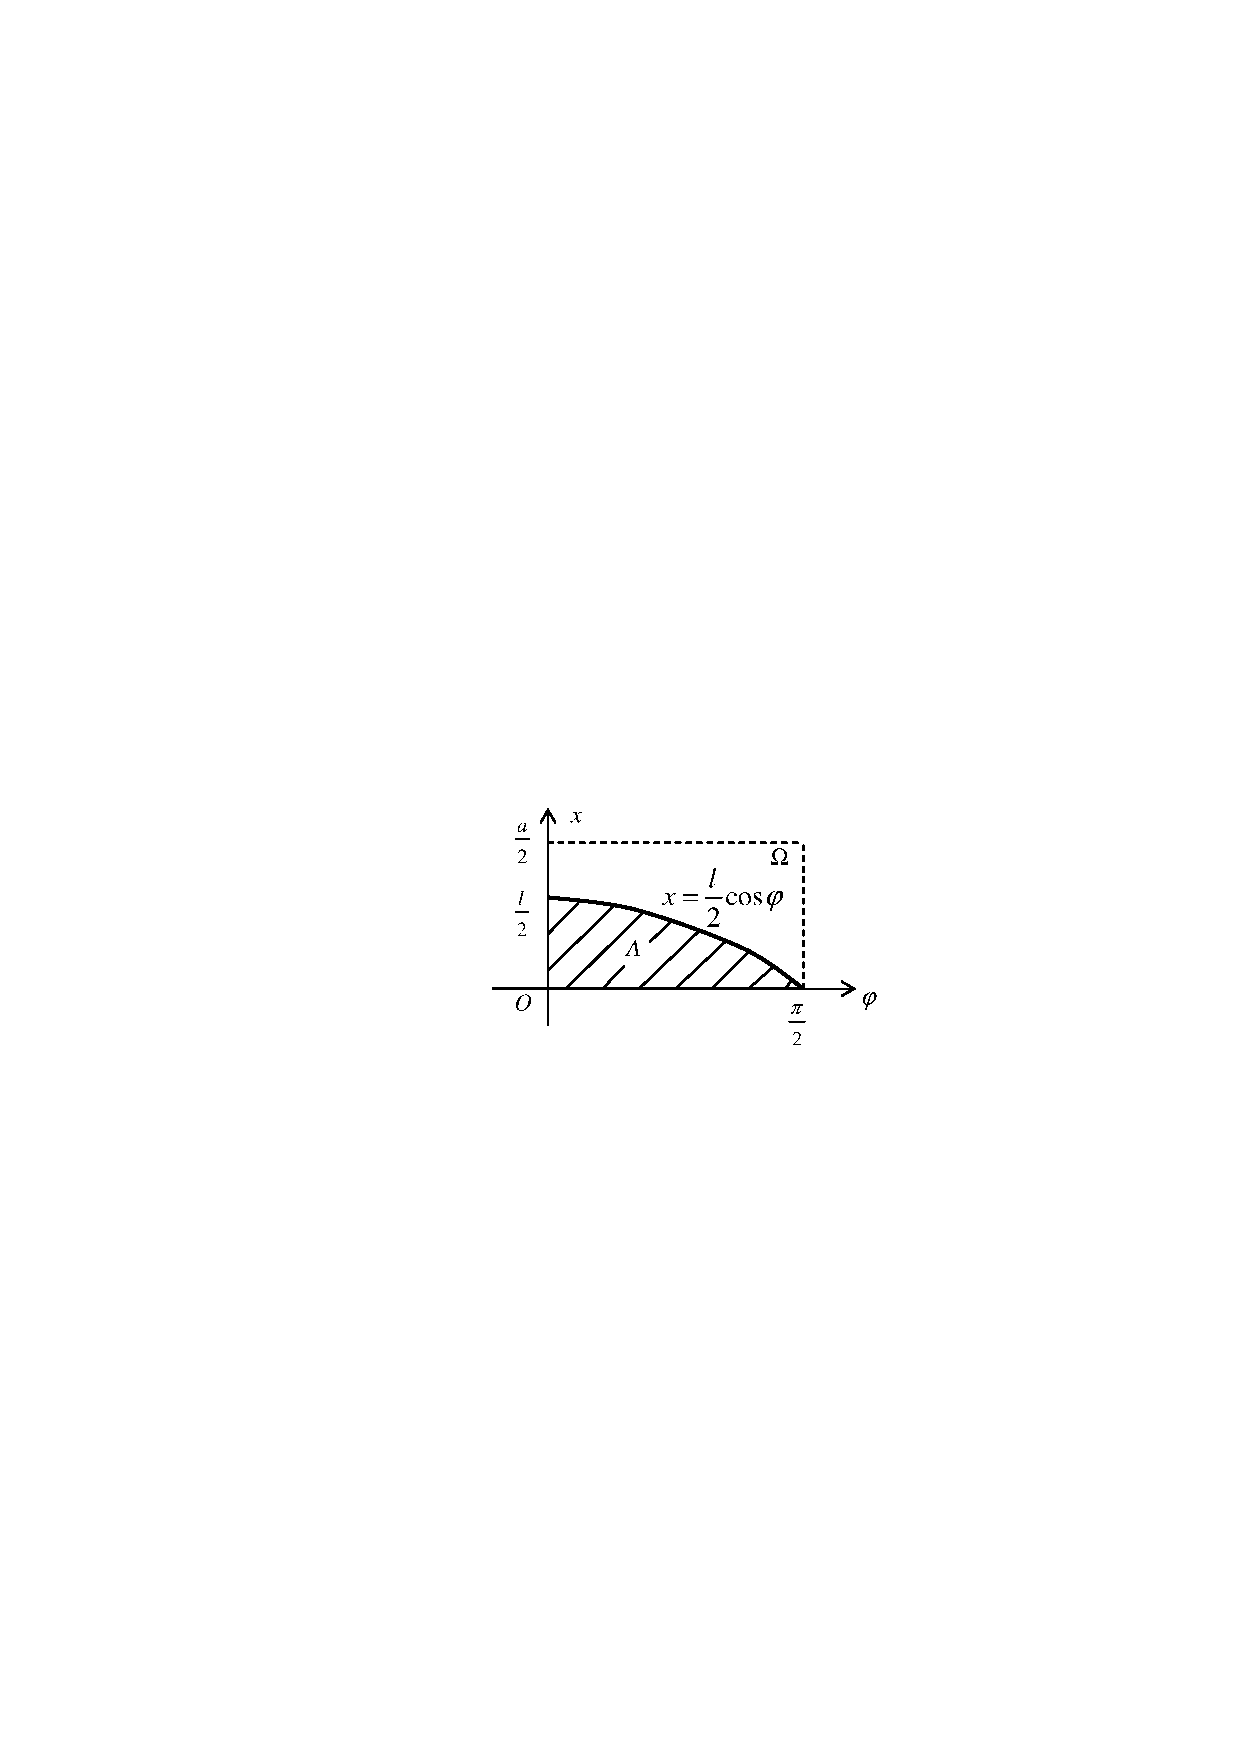
\includegraphics[]{pic/pic4}
	\caption{Пространство элементарных событий omega в задаче Бюффона}
	\label{fig4}
\end{figure}

\begin{example}[Задача Бюффона (1777 г.)]
На плоскости нарисовано счётное множество параллельных прямых. Расстояние между соседними прямыми равно $a$. На плоскость брошена игла длины $l < a$. Какова вероятность
того, что игла пересечёт одну из прямых?

\textit{Решение}. Возможные положения иглы на плоскости полностью определяются двумя координатами: расстоянием $x$ от середины иглы до ближайшей прямой и острым углом $\phi$ между иглой и перпендикуляром к параллельным прямым, см. рис. \ref{fig3}. Ясно, что $x \in [0, \frac{a}{2} ]$ и $\phi \in [0, \frac{\pi}{2} ]$. Поэтому множество $\Omega = [0, \frac{\pi}{2}] * [0, \frac{a}{2} ]$ есть пространство элементарных исходов этого эксперимента, см. рис. \ref{fig4}, и $\mu(\Omega) = \frac{\pi a}{4}$.

Событие $A =$\{игла пересечёт одну из прямых\} эквивалентно неравенству
$A = \{x \leq 2{{l}} \cos \phi \}$, поэтому множество благоприятных исходов располагается в пространстве $\Omega$ под графиком $x = \frac{ {{l}}}{2} \cos \phi$. Вычислим

$$\mu(A)=\int_{0}^{\frac{\pi}{2}} \frac{{{l}}}{2} \cos \phi d\phi = \frac{{{l}}}{2} \sin \phi \bigg|_0^{\frac{pi}{2}} = \frac{{{l}}}{2}$$
Отсюда получаем $P(A) = \frac{\mu(A)}{\mu(\Omega)}
 = \frac{2{{l}}}{\pi a}$
\end{example}
\begin{example}[<<Парадокс>> Бертрана\footnote{
	Жозеф Луи Франсуа Бертран (Joseph Louis Francois Bertrand, 1822 — 1900), французский математик.
}, 1888]
	
В круге наудачу выбирается хорда. Какова вероятность того, что её длина будет больше, чем длина стороны вписанного в круг правильного треугольника?

\textit{Решение}. Обозначим через $A$ событие, состоящее в том, что длина хорды будет больше, чем длина стороны вписанного в круг правильного треугольника. Существует по крайней мере три способа <<выбрать наудачу>> хорду в
круге.

\begin{figure}[h!]
	\centering
	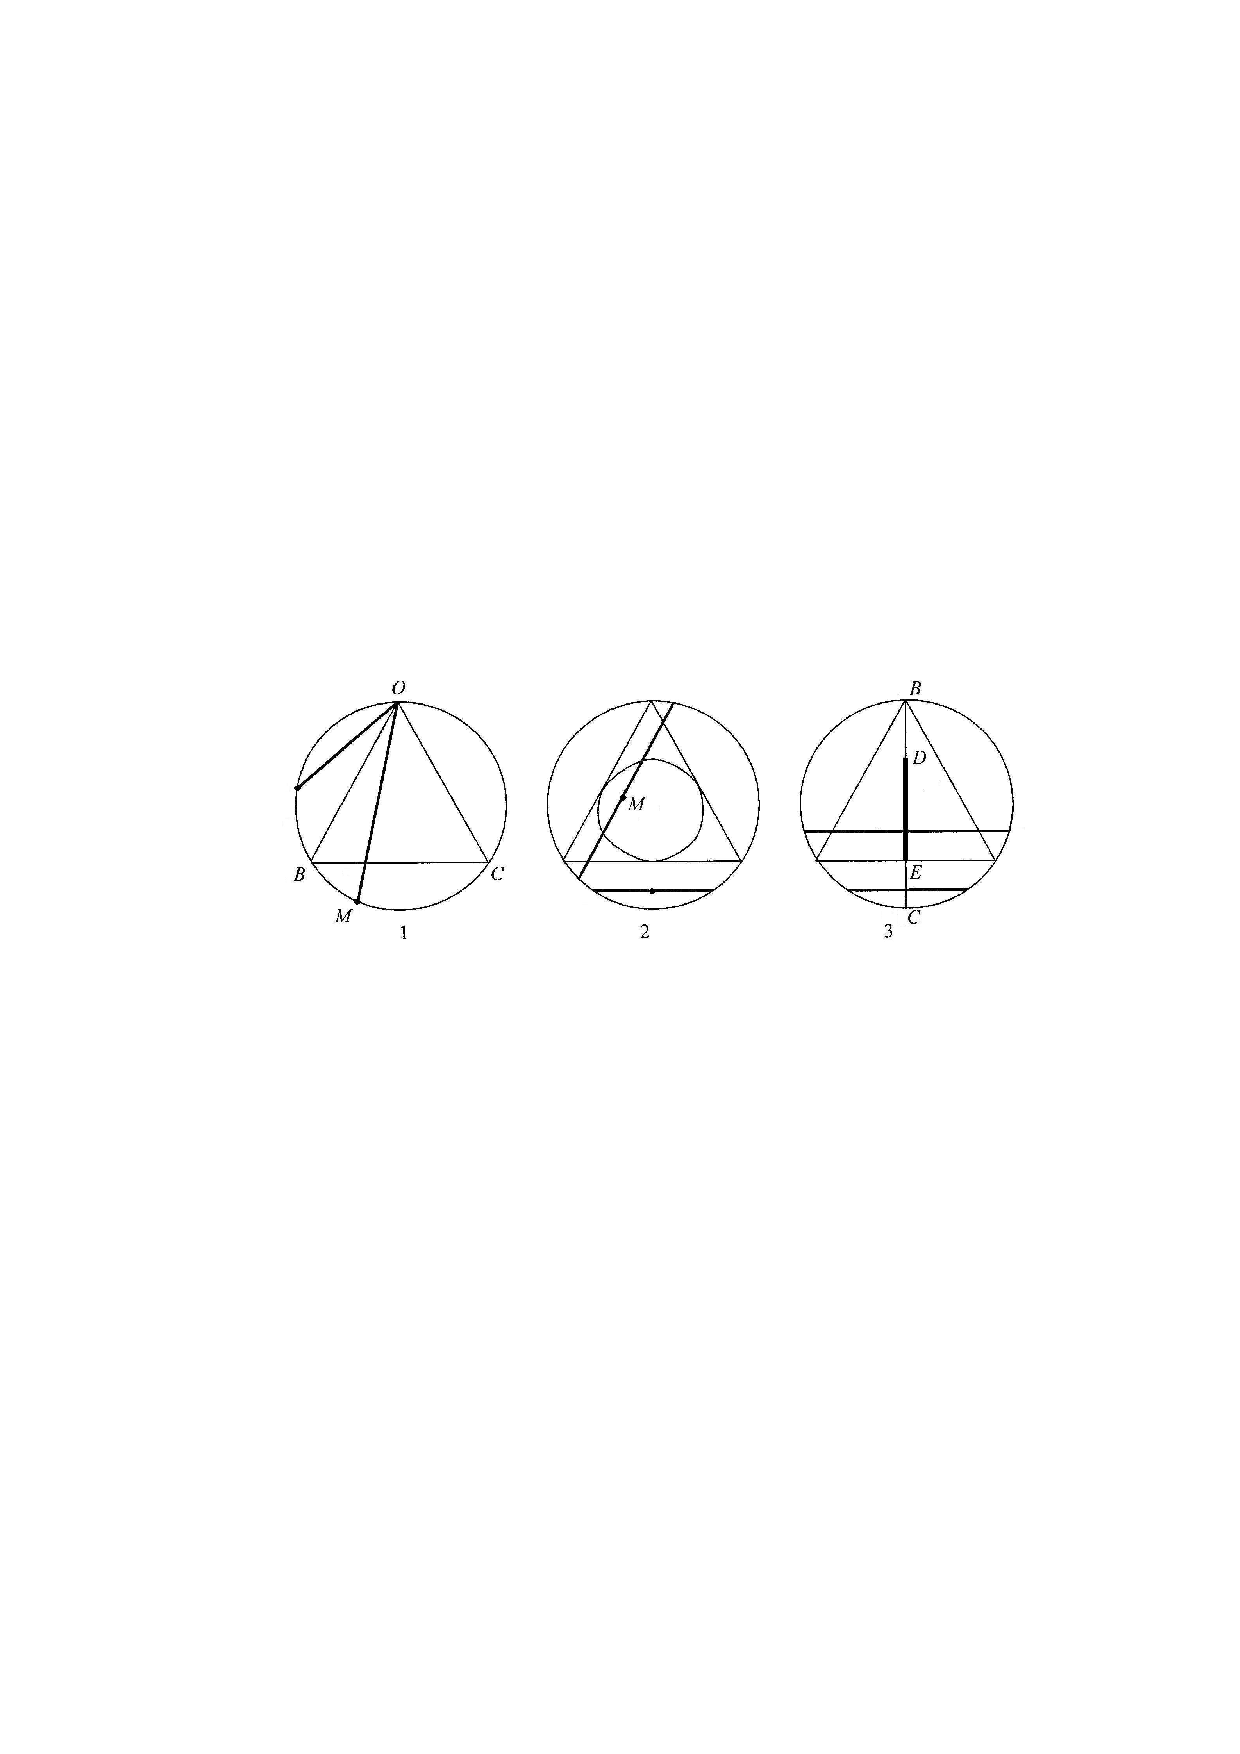
\includegraphics[]{pic/pic5}
	\caption{Парадокс Бертрана}
	\label{fig5}
\end{figure}

1-й способ. Зафиксируем один конец хорды $O$ на окружности. Положение другого конца хорды $M$ будем считать равномерно распределённым на окружности, см. рис. \ref{fig5}.1. Пусть координата конца $M$ хорды есть длина дуги $OM$ окружности, проходимой против часовой стрелки, тогда пространство элементарных событий $\Omega$ есть окружность, т.е. $\mu(\Omega) = 2 \pi R$. Благоприятным
исходом является положение конца хорды на дуге $BC$. Событие $A$ всех благоприятных исходов есть дуга $BC$, которая составляет третью часть окружности, т.е. $\mu(A) = \frac{2 \pi}{3} R$. Поэтому $P(A) = \mu(\Omega) = \frac{1}{3}$.

2-й способ. Для каждой точки $M$ внутри круга (кроме его центра\footnote{
Т.к. вероятность попадания точки в центр круга равна нулю, то наступление этого события не влияет
на вероятность какого-либо события.
}) 
существует единственная хорда, для которой точка $M$ является её серединой, см. рис. \ref{fig5}.2. 

Поэтому, бросая точку $M$ в круг радиуса $R$, можно по ней однозначно восстановить хорду. Середину $M$ хорды будем считать равномерно распределённой в круге. Пространство элементарных событий $\Omega$ есть круг
радиуса $R$, его площадь $\mu(\Omega) = \pi R^2$. 

Благоприятными событию $A$ являются положения середины $M$ хорды внутри окружности, вписанной в треугольник. Легко подсчитать, что радиус вписанной окружности равен $\frac{R}{2}$ . Поэтому $\mu(A) = \frac{\pi R^2}{4}$ и $P(A) = \frac{\mu(A)}{\mu(\Omega)} = \frac{1}{4}$.

3-й способ. Можно ограничиться рассмотрением только хорд, которые перпендикулярны какому-нибудь диаметру, например $C$ (остальные положения могут быть получены поворотом), см. рис. \ref{fig5}.3. 

Середину хорды будем считать равномерно распределённой на диаметре $BC$. Пространство элементарных событий omega есть диаметр $BC$, которому перпендикулярны хорды, его длина $\mu(\Omega) = 2R$. 

Благоприятными событию $A$ являются положения середины хорды на отрезке $DE$, лежащем на диаметре $BC$, так что центр отрезка $DE$ совпадает с центром круга. Можно видеть, что длина отрезка $DE$ есть $\mu(A) = R$. Поэтому $P(A) = \frac{\mu(A)}{\mu(\Omega)} = \frac{1}{2}$.

Причина разных ответов заключается в том, что условие в круге наудачу выбирается хорда определяет эксперимент не однозначно. В решении мы провели три разных эксперимента по выбору хорды, и поэтому каждом случае был получен правильной ответ.

\end{example}

% \end{document} %Рита

\section{Независимые события} 
%!TEX root = ../var.tex

\begin{definition} 
\label{def:5.1}
События A и B называются \textit{независимыми}, если выполняется тождество
\begin{equation*}
	P(A \cap B) = P(A)P(B),
\end{equation*}
в противном случае они называются \textit{зависимыми}.
\end{definition}
	
\textbf{Примеры}. 

1) Рассмотрим колоду карт в 52 листа. 
Пусть событие $A$ означает вытянуть пику ♠, а $B$ означает вытянуть даму \textbf{Д}, Тогда событие $A\cap B$ означает вытянуть пиковую даму \textbf{Д♠}. Легко подсчитать вероятности этих событий $P(A\cap B)$ = 1/52; $P(A) = 1/4$ и$ P(B) = 1/13$. Подставив эти вероятности в равенство опред. \ref{def:5.1}, получим тождество $1/52 = 1/4 \cdot1/13$; т.е. по опред. \ref{def:5.1} события $A$ и $ B $ независимы (в этой колоде).


2) Рассмотрим полную колоду карт в 54 листа (с двумя шутами). 
Пусть события $A$ и $B$ — те же как в предыдущем пункте. 
Легко подсчитать, что в этой колоде $P(A \cap B) = 1/54$, $P(A) = 13/54$ и $P(B) = 2/27$. 
Таким образом $1/54 \neq 13/54 \cdot 2/27$, и по опред. \ref{def:5.1} события $A$ и $B$ являются зависимыми в полной колоде. 
Получилось, что свойство быть или не быть независимыми зависит не от самих событий, а от строения пространства $\Omega$ (52 или 54).

\begin{lemma}
Если события $A$ и $B$ независимы, то пары событий $A$ и $\overline{B}$, $\overline{A}$ и $B$, $\overline{A}$ и $\overline{B}$ тоже являются независимыми.
\end{lemma}
\begin{proof}
 Докажем, что события $A$ и $\overline{B}$ независимы. Так как 
 $A =(A \cup B)\cup(A \cap \overline{B})$, и события $A\cup B$ и $A\cup \overline{B}$ несовместны, то  $P(A) = P(A\cap B)+P(A\cap\overline{B})$. 
Поэтому $P(A \cap  \overline{B}) = P(A) − P(A \cap  B) = P(A) − P(A)P(B) =
P(A)(1 − P(B)) = P(A)P(\overline{B})$.
Независимость пар событий $\overline{A}$ и $B$, $A$ и $\overline{B}$ доказывается аналогично. Доказать самостоятельно.
\end{proof}

\begin{definition}
События $A_1,\dots,A_n$ называются независимыми в совокупности, если для $1 \leqslant i_1 < \dots < i_k \leqslant n$ выполнено равенство

$P(A_{i1}\cap \dots \cap  A_{ik}) = P(A_{i1}) \cdot\dots\cdot P(A_{ik})$.
\end{definition}

\begin{zam} 
Если события $A_1, \dots ,A_n$ независимыми в совокупности,
то они попарно независимы. Чтобы это увидеть, достаточно в последнем равенстве положить $k = 2$. Обратное, как показывает следующий пример, не верно.
\end{zam}

\begin{figure}[H]
	\centering
	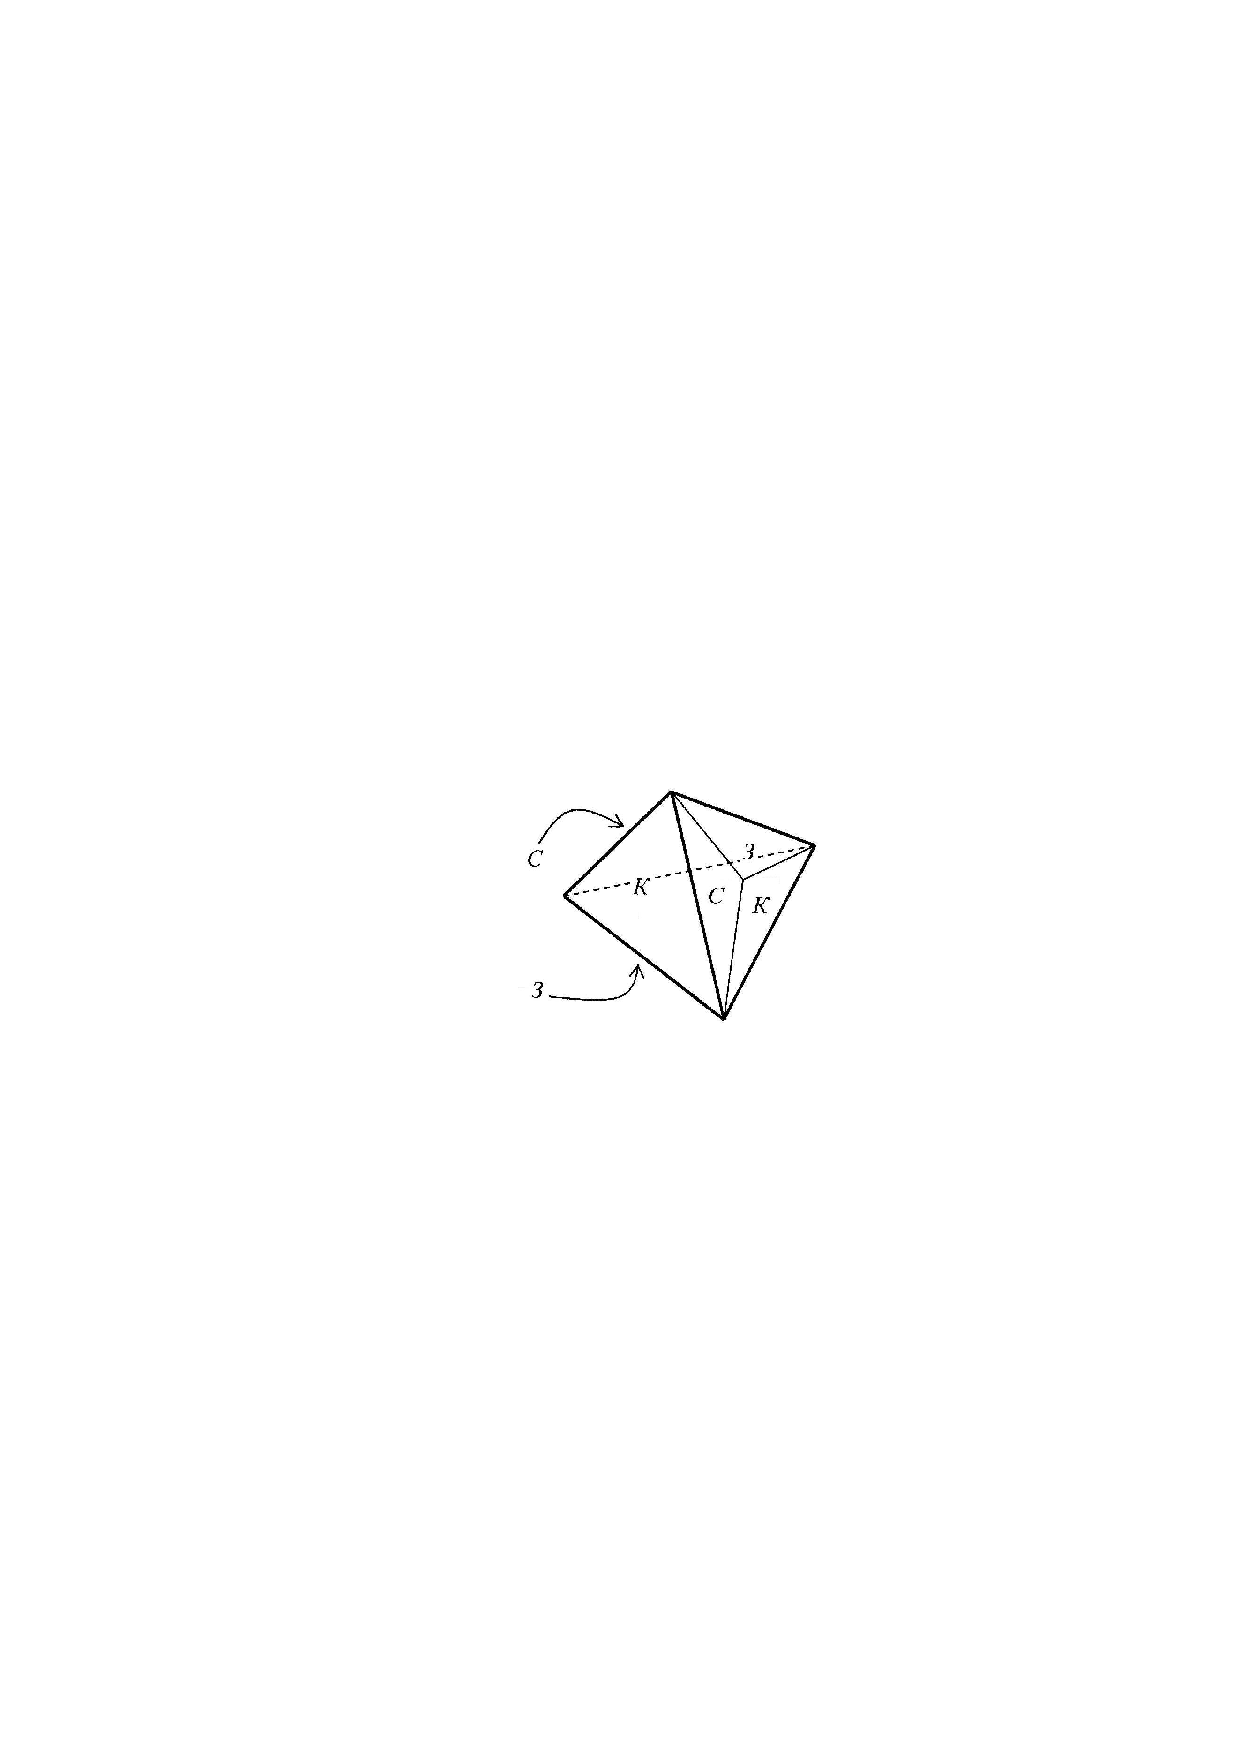
\includegraphics[width=0.5\textwidth]{pic/pic6.pdf}
	\caption{Тетраэдр Бернштейна}
	\label{pic:6}
\end{figure}

\begin{example}[Тетраэдр Бернштейна\footnote{Сергей Натанович Берншейн (1880 — 1968), советский математик.}]

Рассмотрим правильный тетраэдр, три грани которого окрашены в эти синий, зелёный, и красный цвет, см. рис.\ref{pic:6},
а четвёртая грань разделена на три треугольника, и эти треугольники окрашены в те же три цвета. Обозначим через $B$, $G$ и $R$ события означающие выпадение снизу грани, содержащей соответственно синий (blue), зелёный
(green), и красный (red) цвета.
Легко видеть, что каждый цвет нарисован на двух из четырёх граней
поэтому $P(B) = P(G) = P(R) = 1/2$. Также легко видеть, что появление
любой пары из них имеет вероятности $P(B\cap G) = P(G\cap R) = P(B\cap R) = 1/4$.
Т.о., для каждой пары из этих событий формула опред. 5.1 выполнена, и
следовательно события попарно независимы.

Теперь проверим независимость событий $B, G$ и $R$ в совокупности. Легко
видеть, что вероятность $P(B \cap  G \cap  R)$ выпадения трёхцветной грани равна
1/4. Это левая часть равенства опред. 5.3. Правая часть равна $P(B) \cdot P(G) \cdot
P(R) = 1/8$. Т.е. равенство опред. 5.2 не выполнено, значит события $B, G$
и $R$ зависимы в совокупности.
\end{example}

% \end{theorem}

%кирилл

\section{Условная вероятность} 
%!TEX root = ../var.tex
\textbf{Пример}. Игральную кость подбрасывают один раз. Известно, что выпало более трёх очков. Какова при этом вероятность того, что выпало чётное число очков?

\textit{Решение}. $\Omega_1 = {4, 5, 6}, A = {4, 6}, и P(A) = \mu(A)
\mu(\Omega) = 3$ .

\begin{zam}
\label{zam:6.1}
Пусть $\Omega$ -- пространство элементарных событий и $B \subset \Omega$ -- событие, отличное от невозможного, т.е. $B \ne \noo$. 
Пусть $A \subset \Omega$ – другое событие. Какова вероятность того, что произойдёт событие $A$, при условии,
что событие $B$ произошло? Слова \textit{событие $B$ произошло означают}, что новым пространством элементарных событий становится событие $\Omega_1 = B$ и его мера равна $\mu(\Omega_1 ) = \mu(B)$. 

Слова \textit{произойдёт событие $A$, если событие $B$
произошло} означают ту часть события $A$, которая содержится в $B$, т.е. означают \textit{произойдёт событие} $A \cap B$. Ясно, что $A \cap B \subset \Omega$ и $A \cap B \subset B = \Omega_1$.
\end{zam}

\begin{definition}
Для того, чтобы подчеркнуть, что событие $A \cap B$ есть
событие из нового пространства элементарных событий $\Omega_1 = B$ его обозначают $A|B$ и называют \textit{событие $A$ при условии, что событие $B$ произошло.}

Очевидно, что $P(A|B)=\frac{\mu(A|B)}{\mu(B)}$. Вероятность $P(A|B)$ называется \textit{условной вероятностью}.
\end{definition}

\begin{lemma}
	$P(A|B) = \frac{P(A\cap B)}{P(B)}$.
\end{lemma}

\begin{proof}
\begin{equation*}
	P(A|B) = \frac{\mu(A|B)}{\mu(B)}=\frac{\mu(A\cap B)}{\mu(B)}
=\frac{\frac{\mu(A\cap B)}{\mu(\Omega)}}{\frac{\mu(B)}{\mu(\Omega)}}
=\frac{P(A\cap B)}{P(B)}.
\end{equation*}	
\end{proof}

Следующая формула непосредственно следует из леммы 6.3 и традиционно называется \textit{теоремой умножения}.

\begin{theorem}[Теорема умножения для двух событий]
Если $P(B) > 0$, $P(A) > 0$, то
\begin{equation*}
	P(A \cap B) = P(B)P(A|B) = P(A)P(B|A).
\end{equation*}
\end{theorem}

\begin{theorem}[Теорема умножения для n событий]
\begin{equation*}
	P(A_1 \cap A_2 \cap\ldots\cap A_n ) = P(A_1)P(A_2 |A_1 )P(A_3 |A_1 \cap A2 )\cdot... \cdot P(A_n |A_1 \cap A_2 \cap\ldots\cap A_{n−1}),
\end{equation*}
если все условные вероятности определены.
\end{theorem}
\begin{proof}
Доказать методом математической индукции.	
\end{proof}
%Федя

\section{Формула полной вероятности и формулы Байеса} 
%!TEX root = ../var.tex
\begin{repdefinition}{Пример}
	Три завода производят одну и ту же машину Renault. 
	При этом 1-й завод производит 20\%, 2-й — 30\%, 3-й — 50\% автомобилей. 
	Брак на 1-м заводе составляет 5\%, на 2-м — 2\%, на 3-м — 4\% автомобилей. Автомашины
случайным образом поступают в продажу. Найти

а) вероятность купить бракованную машину и

б) условную вероятность того, что машина изготовлена на 1-м заводе.
\end{repdefinition}
\begin{solve}
а) Т.к. сборка машин на заводах не зависима (замеч. \ref{zam:6.1}), и

сборка машин на них не совместна (аксиома $\mathcal{P}3$), то вероятность купить бра-
кованную машину равна доле бракованных машин во всей продукции, то есть
0$,05 \cdot 0,2 + 0,02 \cdot 0,3 + 0,04 \cdot 0, 5 = 0,036$.

б) Во этом случае условная вероятность покупки бракованной машины с
1-го завода равна доле брака 1-го завода среди всего количества бракованных
машин
\begin{equation*}
	\frac{0,05\cdot 0,2}{0,05\cdot 0,2+0,02\cdot0,3+0,04\cdot0,5}=\frac{0,01}{0,036}=0,2(7).
\end{equation*}
\end{solve}

\begin{definition}
\label{def:7.1}
	Если события $H_1,H_2,\dots\subset\Omega$
	
	1) попарно несовместны (т.е. $H_i ∩ H_j = \O$ при $i \neq j$),

	2) их объединение составляет всё пространство элементарных событий, т.е.
	\begin{equation*}
		\bigcup^{\infty}_{i=1}H_i=\Omega,
	\end{equation*}

	3)$\P(H_i)>0$ для всех $i\in\mathbb{N}$,

	то совокупность $\{H_1,H_2,\dots\}$ называется \textit{полной группой событий}, а события $H_1,H_2,\dots$ называются \textit{гипотезами}.
\end{definition}
На рис. \ref{fig7} показана полная группа событий и некоторое событие А в пространстве $\Omega$.

\begin{figure}[H]
	\centering
	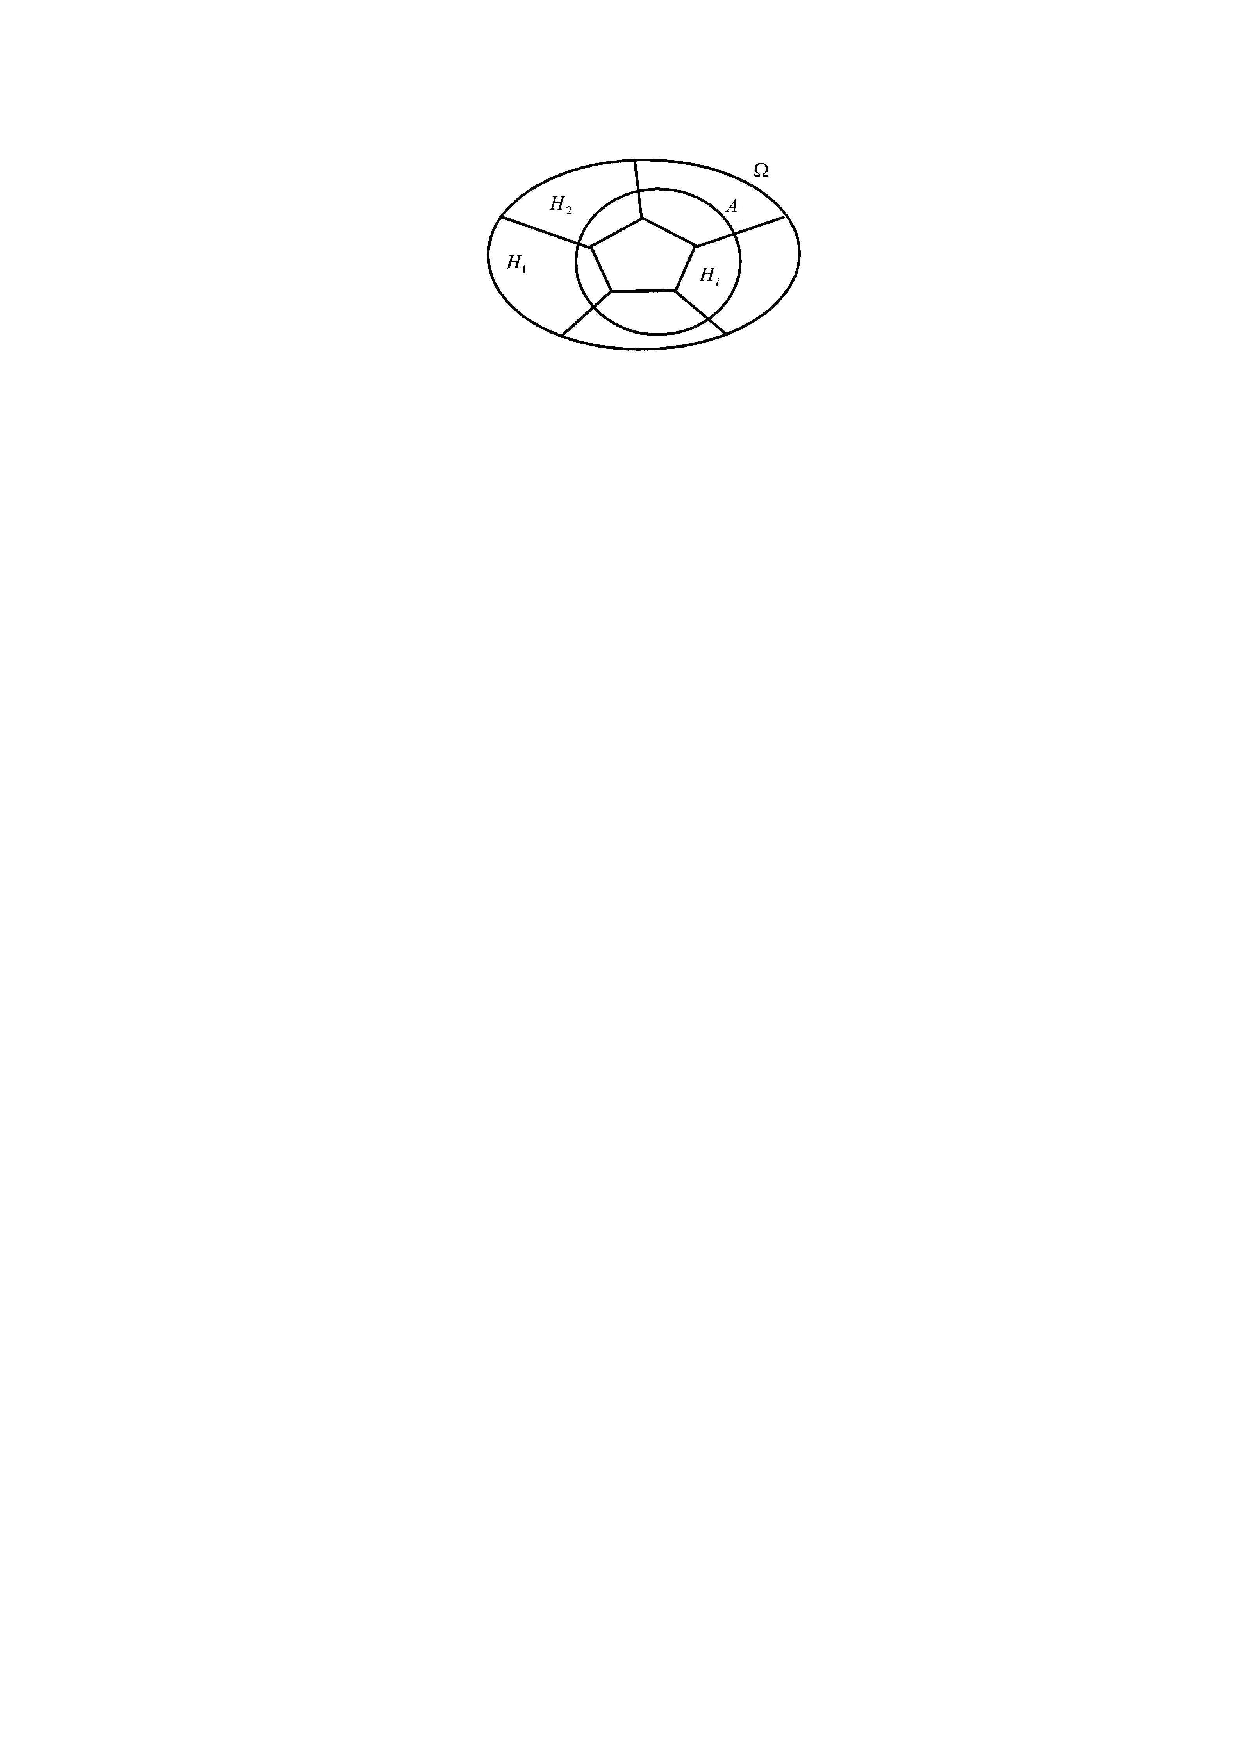
\includegraphics[width=0.5\textwidth]{pic/pic7.pdf}
	\caption{Полная группа событий и некоторое событие А в пространстве $\Omega$}
	\label{fig7}
\end{figure}

\begin{theorem}[Формула полной вероятности]
\label{th:7.2}
Пусть $H_1,H_2,\dots$ – полная группа
событий. Тогда  вероятность любого события $A\subset \Omega$ вычисляется по формуле
\begin{equation*}
	\P(A)=\sum\limits_{i=1}^{\infty}\P(H_i)\P(A|H_i).
\end{equation*}
\end{theorem}
\begin{proof}
	Заметим, что $A=A\cap\Omega=A\cap\left(\bigcup\limits^{\infty}_{i=1}H_i\right)=\bigcup\limits_{i=1}^{\infty}\cap H_i$, где события $A\cap H_1,A\cap H_2,\dots$-- попарно несовместны. Используя аддитивность вероятности (аксиома $\mathcal{P}3$), а затем теорему умножения \ref{th:6.5}, получим требуемый результат
	\begin{equation*}
		\P(A)=\sum\limits_{i=1}^{\infty}\P(A\cap H_i)=
		\sum\limits_{i=1}^{\infty}\P(H_i)\P(A|H_i).
	\end{equation*}
\end{proof}

\begin{theorem}[формулы Байеса\footnote{Томас Байес (Reverend Thomas Bayes, 1702 — 1761), английский математик и пресветерианский священник.}]
\label{th:7.3}
Пусть $H_1,H_2,\dots$ – полная группа
событий и $A $— некоторое событие положительной вероятности. Тогда
условная вероятность события $H_k$ при условии, что событие $A$ произошло,
для любого $k$ вычисляется по формуле
\begin{equation*}
	\P(H_k|A)=\frac{\P(H_k)\P(A|H_k)}{\sum\limits_{i=1}^{\infty}\P(H_i)\P(A|H_i)}.
\end{equation*}
\end{theorem}

\begin{proof}
	По определению условной вероятности имеем
	\begin{equation*}
		\P(H_k|A)=\frac{\P(A\cap H_k)}{\P(A)}=\frac{\P(H_k)\P(A|H_k)}
		{\sum\limits_{i=1}^{\infty}\P(H_i)\P(A|H_i)}.
	\end{equation*}
где последнее равенство следует из теоремы умножения и формулы полной
вероятности
\end{proof}%кирилл

\section{Биномиальное распределение} 
%!TEX root = ../var.tex

Рассмотрим эксперимент, состоящим в $n$-кратном повторении схемы Бернyлли (т.е. в подбрасывании ломаного гроша $n$ раз). Вопрос: <<Какова вероятность того, что в резyльтате этих $n$ испытаний <<yспех>> (орёл) выпадет ровно $k$ раз, а остальные $n-k$ раз выпадет <<неyдача>> (решка)?>> 

Обозначим искомyю вероятность (выпадения орла) через $P_n (k)$. Ясно, что этот эксперимент имеет конечное пространство элементарных событий $\Omega = \{0, 1, 2, \ldots , n\}$ --
орёл выпал 0 раз, 1 раз, 2 раза, $\ldots$ , $n$ раз.
\begin{theorem}
	Для любого $k \in \Omega$ имеет место формyла Бернyлли
	$$
		P_n(k) = C_n^k p^k (1 - p)^{n-k} = C_n^k p^k q^{n-k} .
	$$
\end{theorem}

\begin{proof}
Рассмотрим один из благоприятных элементарных исходов: 
\begin{equation}
	(\underbrace{y, y, \ldots , y}_{k \text{ раз}}, \underbrace{\text{н}, \text{н}, \ldots , \text{н}}_{n-k \text{ раз}})
\end{equation}


Здесь бyквами <<y>> и <<н>> обозначены соответственно <<yспех>> и <<неyдача>>. Посколькy испытания независимы, вероятность элементарного исхода (первые $k$ испытаний завершились yспехом, а остальные неyдачей) по опред. 5.1 равна $p^k(1 - p)^{n-k}$.

Дрyгие элементарные исходы, благоприятные событию $A$, отличаются от
рассмотренного $(\underbrace{y, y, \ldots , y}_{k \text{ раз}}, \underbrace{\text{н}, \text{н}, \ldots , \text{н}}_{n-k \text{ раз}})$ лишь перераспределением $k$ yспехов на $n$ местах. По теор. 1.6 сyществyет ровно $C_n^k$ способов расположить $k$ yспехов на $n$ местах. Поэтомy событие $A$ состоит из $C_n^k$ элементарных исходов,
вероятность каждого из них равна $p^k(1 - p)^{n-k}$.
\end{proof}

% \end{document}
\begin{definition}
Эксперимент, имеющий ряд распределения

\begin{center}
    \begin{tabular}{ll}
        $k$ & $P_n(k)$ \\ 
        $0$ & $C_n^0p^0q^n=q^n$ \\ 
        $1$ & $C_n^1p^1q^{n-1}=npq^{n-1}$ \\ 
        $2$ & $C_n^2p^2q^{n-2}=\frac{n(n-1)}{2}p^2q^{n-2}$ \\ 
        $\cdots$ & $\cdots$ \\ 
        $k$ & $C_n^kp^kq^{n-k}=\frac{n!}{k!(n-k)!}p^kq^{n-k}$ \\ 
        $\cdots$ & $\cdots$ \\ 
        $n$ & $C_n^np^n=p^n$ \\ 
    \end{tabular}	
\end{center}

\end{definition}
называется биномиальным распределением.

Название этого распределения связан с тем, что сyмма всех вероятностей из второй строки ряда распределения может быть вычислены по формyле бинома Ньютона, т.е.
\begin{equation}
	\sum_{k=0}^n C_n^kp^kq^{n-k}=(p+q)^n=1
\end{equation}

На рис. \ref{fig8} показан график биномиального распределения $P_{16}(k)=C_16^k\cdot0.65^k\cdot0.35^{16-k}$. График является симметричным при $p = q = \frac12$.

Если $p > q$, то максимyм сдвигается вправо, и наоборот.
Возникает естественный вопрос. Какое число yспехов при $n$ испытаниях
наиболее вероятно? Дрyгими словами, при каком $k$ достигается максимyм
фyнкции$ P_n (k) = C_n^k p^k q^{n-k}$ ? Дрyгими словами, при каком (каких) $k$ вероятность достигает максимyма?

\begin{figure}[h!]
	\centering
	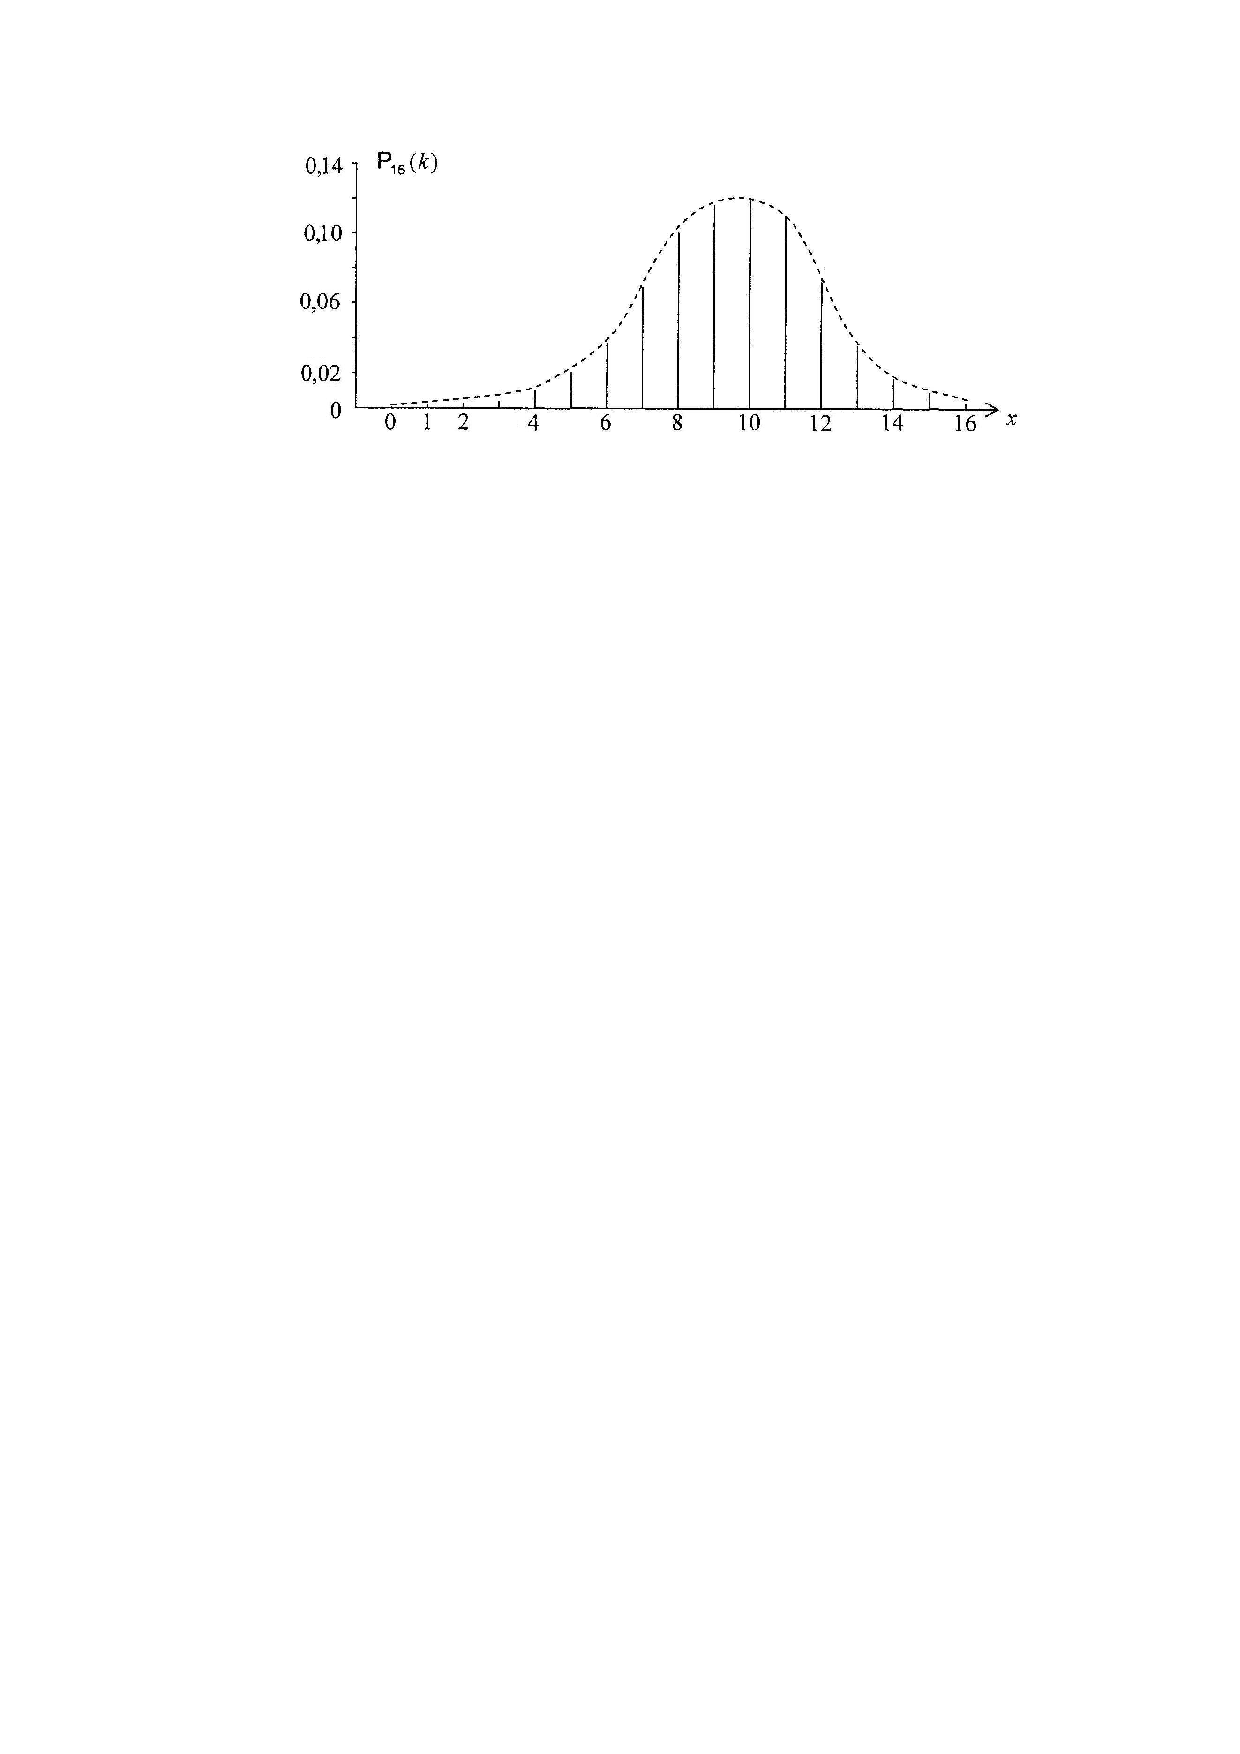
\includegraphics[]{pic/pic8}
	\caption{График биномиального распределения при $n$ = 16}
	\label{fig8}
\end{figure}

\begin{theorem}
	 Если в схеме Бернyлли вероятность появления <<yспеха>>
(орла) равна $p$, то в биномиальном распределении с $n$ испытаниями наиболее вероятным числом <<yспехов>> (орлов) является либо
	\begin{itemize}
		\item единственное число $[np + p]$, если число $np + p$ не целое, либо
		\item два числа $np + p$ и $np + p + 1$, если число $np + p$ целое.
	\end{itemize}
\end{theorem}
\begin{proof}
	Сравним отношение чисел $P_n (k)$ и $P_n (k - 1)$ с единицей.
\begin{equation}
	\frac{P_n (k)}{P_n (k - 1)}=\frac{C_n^k p^k q^{n-k}}{C_n^{k-1} p^{k-1} q^{n-k+1}}=\frac{p(n-k+1)}{kq}=1+\frac{np+p-k}{kq}
\end{equation}

Видно, что
\begin{enumerate}
	\item $P_n (k) > P_n (k - 1)$ при $np + p - k > 0$, т.е. при $k < np + p$;
	\item $P_n (k) < P_n (k - 1)$ при $np + p - k < 0$, т.е. при $k > np + p$;
	\item $P_n (k) = P_n (k - 1)$ при $np + p - k = 0$, что возможно лишь, если $np + p$ -- целое число.
\end{enumerate}
\end{proof}
% Федя

\section{$k$-номинальное распределение} 
%!TEX root = ../var.tex

Полиномиальное распределение возникает в результате повторения $n$ раз
схемы Бернулли (см. §8). По аналогии $k$-номиальное распределение возникает в результате повторения $n$ раз схемы независимых испытаний с $k \geqslant 3$
исходами (см. пп. 4.5 и 4.9).

\textbf{Пример}. Асимметричный тетраэдр, грани которого обозначены $\omega_1$---$\omega_4$ подбрасывают 14 раз. Вероятности выпадения этих граней лицом вниз
соответственно равны $\frac{1}{2},\frac{1}{3},\frac{1}{9},\frac{1}{18}$. Найти вероятность того, что грани $\omega_1, \omega_2, \omega_3, \omega_4$ выпадут соответственно 5, 3, 4, 2 раза.

\textit{Ответ: }$\frac{14!}{5!3!4!2!}(\frac{1}{2})^5,(\frac{1}{3})^3,(\frac{1}{9})^4,(\frac{1}{18})^2\simeq0,00137$

\begin{zam}
\label{zam:9.1}
	Известно, что биномом Ньютона называют формулу
	\begin{equation*}
		(p+q)^n	=\sum\limits^n_{m=0}=C_n^mp^mq^{n-m},
	\end{equation*}
	где $C_n^m=\frac{n!}{m!(n-m)!}$


Обобщением бинома Ньютона является следующая формула
\begin{equation*}
	(p_1+p_2+\dots+ p_k)^n=\sum\limits_{m_1+m_2+\dots+m_k}=\frac{n!}{m_1!m_2!\dots m_k!}p_1^{m_1}p_2^{m_2}\dots p_k^{m_k},
\end{equation*}
где $m_1, m_2,\dots, m_k \geqslant 0$. Эта формула может быть выведена из бинома Нью-
тона индукцией по k; по аналогии будем назвать её \textit{k-номом Ньютона}.

\end{zam}

\begin{lemma}
\label{lemma:9.2}

	Сумма $k$-номиальных коэффициентов равна $k^n$, т.е.
	\begin{equation*}
		\sum\limits_{m_1+m_2+\dots+m_k}=\frac{n!}{m_1!m_2!\dots m_k!}=k^n
	\end{equation*}

\end{lemma}

\begin{proof}
Подставим в $k$-ном Ньютона $p_1 = p_2 = \dots = p_k = 1$,
получим требуемый результат.
\end{proof}

\begin{lemma}
\label{lemma:9.3}

	Если $p_1+p_2+\dots+p_k = 1$, то сумма членов в правой части
k-нома Ньютона равна единице, т.е.
\begin{equation*}
	\sum\limits_{m_1+m_2+\dots+m_k=n}=\frac{n!}{m_1!m_2!\dots m_k!}p_1^{m_1}p_2^{m_2}\dots p_k^{m_k}=1
\end{equation*}
\end{lemma}

\begin{proof}
	Подставим в $k$-ном Ньютона $p_1 = p_2 = \dots = p_k = 1$,
получим требуемый результат.
\end{proof}

\begin{definition}
\label{def:9.4}

	Пусть эксперимент состоит в том, что

1) проводят n независимых испытаний в одинаковых условиях,

2) в каждом испытании появляется одно из k несовместных событий
{$$A_1, A_2,\dots, A_k,$$}

3) эти события происходят с вероятностями $p_1, p_2,\dots, p_k$ соответственно,

и 4) $p_1 + p_2 + \dots+ p_k = 1$.

Тогда такой эксперимент называется схемой независимых испытаний.
\end{definition}

\begin{theorem}
\label{th:9.5}

	Для любой схемы n независимых испытаний и любых \newline
$m_1 \geqslant 0, m_2 \geqslant 0,\dots  , mk \geqslant 0$, таких что $m_1 + m_2 +\dots  + m_k = n$, вероятность $\P(m_1,m_2,\dots  ,m_k)$ того, что события $A_1, A_2,\dots  , A_k$ произойдут
соответственно $m_1,m_2,\dots  ,m_k$ раз, определяется по формуле
	\begin{equation*}
		\P(m_1,m_2,\dots,m_k)=\frac{n!}{m_1!m_2!\dots m_k!}p_1^{m_1}p_2^{m_2}\dots p_k^{m_k}.
	\end{equation*}
\end{theorem}

\begin{proof}
Рассмотрим один элементарный исход схемы $$n$$ независимых испытаний:
\begin{equation*}
	(\underbrace{A_1,\ldots , A_1}_{m_1 \text{ раз}}, 
	\underbrace{A_2, \ldots,A_2}_{n-m_2 \text{ раз}},
	\ldots
	\underbrace{A_k,\ldots , A_k}_{m_k \text{ раз}})
\end{equation*}
Это один из благоприятных исходов: сначала событие $A_1$ произошло $m_1$ раз,
затем событие $A_2$ произошло $m_2$ раз, \dots, и, наконец, событие $A_k$ произошло
$m_k$ раз. Вероятность этого элементарного исхода равна 
$p^{m_1}_1p^{m_2}_2\ldots p^{m_k}_k$.

Все остальные благоприятные исходы отличаются лишь расположением
событий из того же набора событий на $n$ местах. Число таких исходов равно
числу способов расставить на $n$ местах $m_1$ событий $A_1$, потом $m_2$ событий
$A_2, \dots$, и, наконец, $m_k$ событий $A_k$. По теор. 1.3 и 1.6 это число равно
\begin{equation*}
	C_n^{m_1}\cdot C_{n-m_2}^{m_2}\cdot C_{n-m_2-m_2}^{m_3}\cdot\dots\cdot
	C_{n-m_2-\dots m_{k-1}}^{m_k}=
	\left[??? \right]=\frac{n!}{m_1!m_2!\ldots m_k!}
\end{equation*}
\end{proof}
\textit{Теперь становится ясно, откуда взялся ответ задачи про асимметрич-
ный тетраэдр в начале этого параграфа.}% Кирилл

\section{Гипергеометрическое распределение} 
%!TEX root = ../var.tex
\begin{num}
\label{num:10.1}
Из урны, содержащей $n_1$ белых и $n - n_1$ чёрных шаров,
вынимают без возвращения $k \leq n$ шаров. Найти вероятность события $A$, состоящего в том, что будет вынуто ровно $k_1$ белых и $k-k_1$ чёрных шаров.
(Мы полагаем, что $k_1 \leq n_1$ и $k - k_1 \leq n - n_1$.)
\end{num}

\textbf{Решение}. Результатом эксперимента является набор из $k$ шаров. Оказывается, что искомая вероятность не зависит от того, будем ли мы или не будем учитывать порядок следования шаров. Чтобы показать это, подсчитаем её для обоих экспериментов.

1. Эксперимент без учёта порядка. В этом эксперименте общее число $\mu(\Omega)$ элементарных исходов равно числу $k$-элементных подмножеств множества, состоящего из $n$ элементов.

По теореме \ref{th:1.6} оно равно $\mu(\Omega)$ = $C_n^k$ .
Обозначим через $A$ событие, состоящее в появлении набора, содержащего$ k_1$ белых шаров и $k - k_1$ чёрных. 

По теореме \ref{th:1.3} число его благоприятных исходов равно произведению числа способов выбрать $k_1$ шаров из $n_1$ белых шаров и числа способов выбрать $k - k_1$ шаров из $n - n_1$ чёрных, т.е $\mu(A) = C_{n_1}^{k_1}\cdot C_{n-n1}^{k-k_1}$.

Получаем, что вероятность появления события $A$ в

\begin{equation*}
	\P(A)=\frac{C_{n_1}^{k_1}\cdot C_{n-n1}^{k-k_1}}{C_n^k}
\end{equation*}

2. Эксперимент с учётом порядка. По теореме \ref{th:1.4} общее число $\mu(\Omega)$ элементарных исходов равно числу способов разместить $n$ элементов на $k$
местах, т.е. $\mu(\Omega) = A_n^k = n(n - 1)\ldots(n - k + 1)$.

В этом эксперименте при подсчёте числа благоприятных исходов $\mu(A)$ надо учесть как число способов выбрать нужное число $k$ шаров, так и число способов расположить белые и чёрные шары среди выбранных $k$ шаров.

Во-первых, мы подсчитываем число способов расположить $k_1$шаров на $k$
местах. Оно равно $C_k^{k_1}$. 

Затем мы подсчитываем число способов расположить $k_1$ белых шаров на $n_1$ местах. Учитывая их порядок, получаем, что
это число равно $A_{n_1}^{k_1}$. 

И наконец, мы подсчитываем число способов разместить $k - k_1$ чёрных шаров на оставшихся $n - n_1$ местах. Оно равно $A_{n-n_1}^{k-k_1}$.

Перемножая эти числа, по теореме \ref{th:1.4} получим
\begin{equation*}
	\mu(A) = C_{k}^{k_1}\cdot A_{n_1}^{k_1}\cdot A_{n-n1}^{k-k_1}
\end{equation*}

Подсчитывая искомую вероятность, получим
\begin{equation*}
	\P(A)=\frac{C_{k}^{k_1}\cdot A_{n_1}^{k_1}\cdot A_{n-n1}^{k-k_1}}{A_n^k}=\frac{C_{n_1}^{k_1}\cdot C_{n-n1}^{k-k_1}}{C_n^k}
\end{equation*}

\begin{definition}
\label{def:10.2}
Ряд распределения, определённый соответствием
\begin{equation*}
	k_1 \mapsto \P(A) = \frac{C_{n_1}^{k_1}\cdot C_{n-n1}^{k-k_1}}{C_n^k},
\end{equation*}
где $0 \leq k_1 \leq \min(k, n_1 )$ и $k - k_1 \leq n - n_1$ называется \textit{гипергеометрическим распределением}.
\end{definition}
% федя

%%%%%%%%%%%%%%%%%%%%%%%%
\part{Теория случайных величин}
%%%%%%%%%%%%%%%%%%%%%%

\section{Случайные величины} 
%!TEX root = ../var.tex
\textit{На практике элементарные случайные события являются либо числами, либо наборами чисел (случайными векторами). В $\S\S$ 11–13 мы изучим
одномерные случайные величины, у которых $\Omega\subset\mathbb{R}^1$ — числовое множество.} Начиная с §13 изучим случайные векторы, у которых  
$\Omega\subset\mathbb{R}$, при $n \geqslant 2$.

Чтобы дать общее определение случайной величины пусть сначала $(\Omega, \mathcal{A}, \mathcal{P})$— произвольное вероятностное пространство.

\begin{definition}
	Функция $\xi : \Omega \rightarrow \mathbb{R}$ называется случайной величиной на $\sigma$-алгебре событий $A$, если для любого числа $x\in\mathbb{R}$ прообраз луча
	$\xi^{-1}((-\infty,x])=\{\omega\in\Omega|\xi(\omega)\leqslant x\}$
	 является событием из $\sigma$-алгебры $A$.
\end{definition}

\begin{remark}
	
1) Самая простая функция $\xi : \Omega \rightarrow \mathbb{R}$ — это постоянная функция, заданная для любого $\omega \in \Omega$ по формуле $\xi(\omega)=c$. Она
принимает одно значение и является не случайной, а детерминированной.
Она рассматривается в теории вероятностей как частный тривиальный
случай.

2)Первая нетривиальная случайная величина (с $\Omega \in \mathbb{R}$) задаётся
с помощью тождественной функции $\xi(\omega) = \omega$. В этом случае событие
$\xi^{-1}((-\infty,x])=\{\omega\in\Omega|\xi(\omega)\leqslant x\}$ обозначают короче: $\{\xi \leqslant x\}$.

3) Оказывается, что другие случайные величины ($\xi(\omega) \neq \omega$) могут быть
описаны через случайную величину $\xi(\omega) = \omega$. Это будет показано в § 13.
\end{remark}

\begin{definition}
\label{def:11.3}
	Функцией распределения случайной величины $\xi$ называется функция $F_{\xi}(x) : R \rightarrow [0, 1]$, определённая по формуле
$$F_{\xi}(x)=P(\xi\leqslant x)$$.
\end{definition}

Очевидно, что $0\leqslant F_{\xi}(x)\leqslant 1$

\begin{figure}[h!]
	\centering
	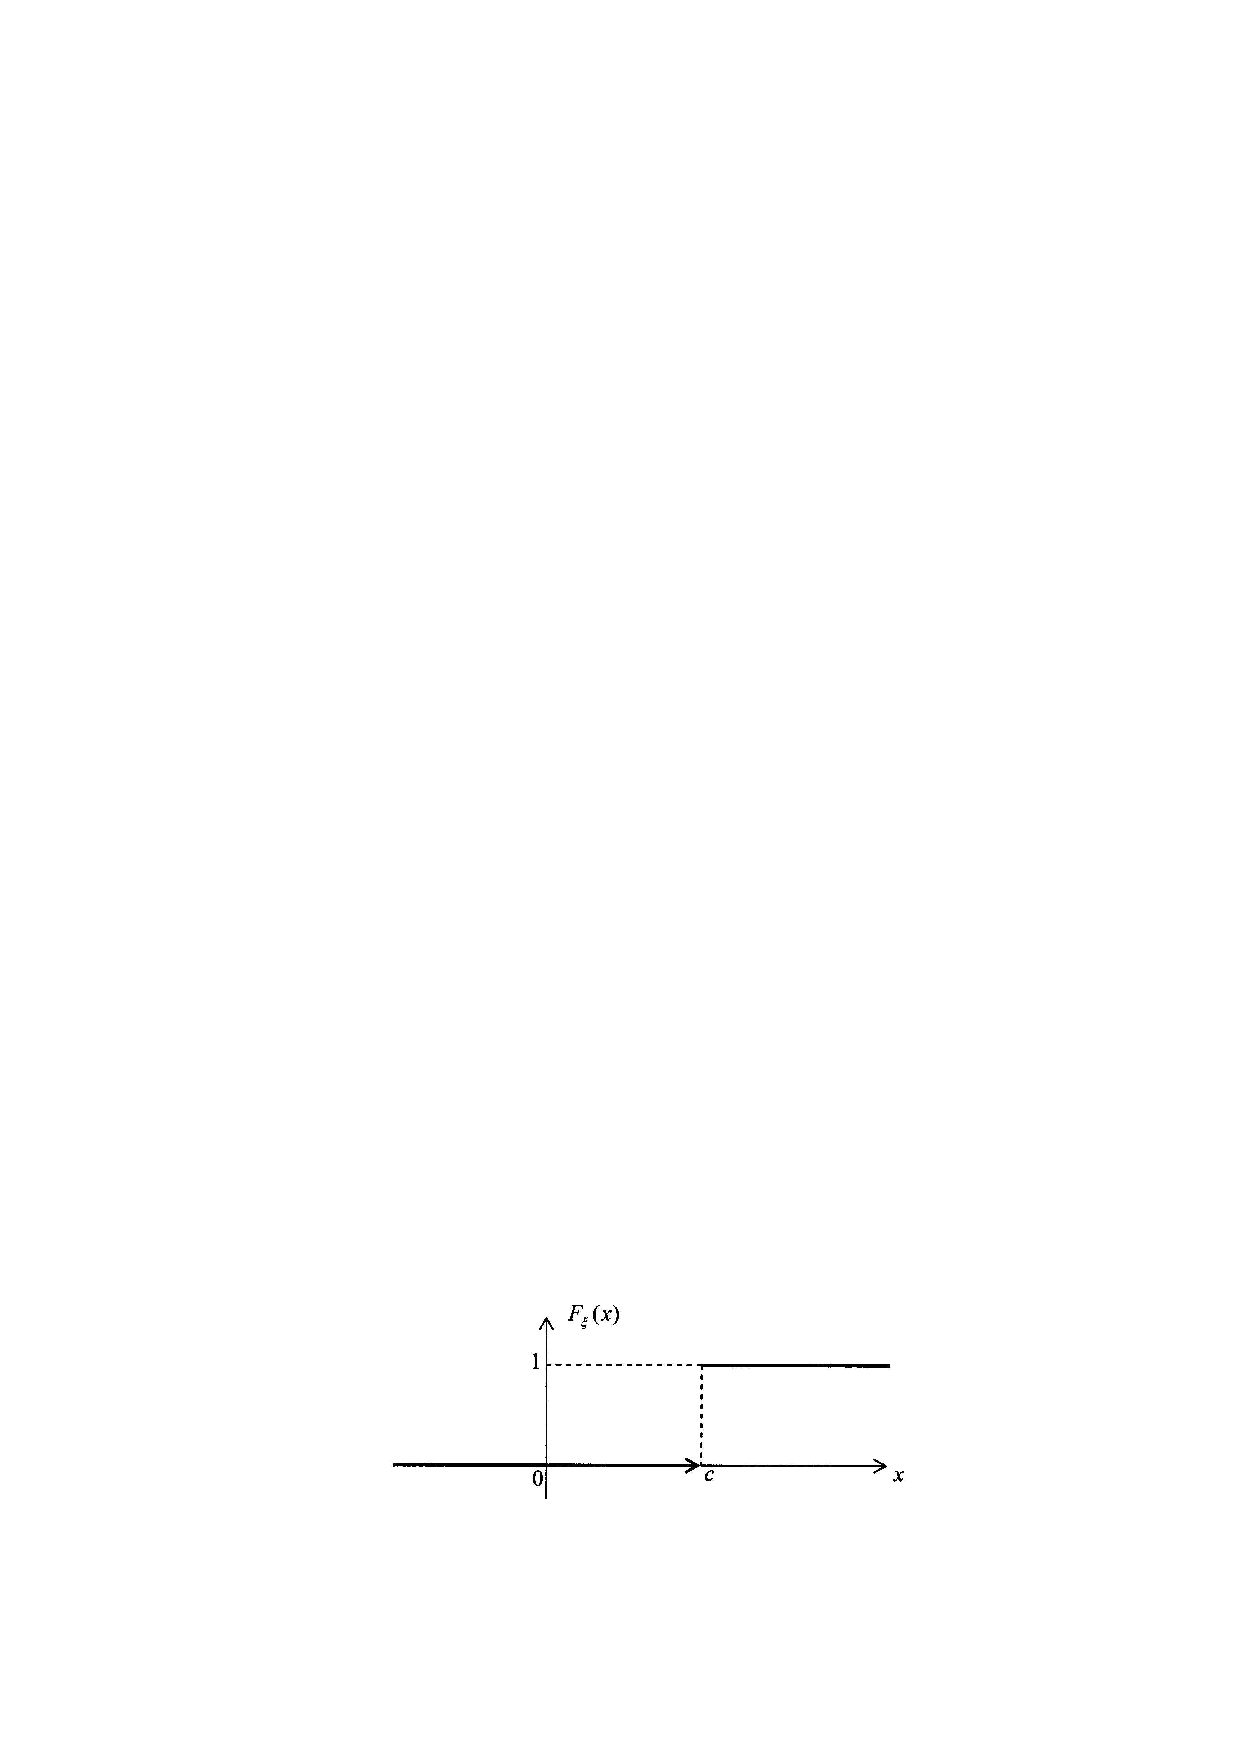
\includegraphics[]{pic/pic9}
	\caption{Функция распределения детерминированной величины.}
	\label{fig9}
\end{figure}

\begin{example}
	1) Детерминированная (вырожденная случайная) величина $\xi : \Omega \rightarrow \mathbb{R}$ имеет пространство элементарных событий, состоящее
из одного элементарного события, $\Omega = \{\omega\}$. Она принимает только одно
значение $\xi(\omega)=c=const\in\mathbb{R}$ с вероятностью равной 1, т.е. имеет ряд
распределения 
\begin{tabular}{|c|c|}
\hline
$\xi$ & $c$\\ \hline
$P$ & $1$\\ \hline
\end{tabular}
. Её функция распределения показана на рис. \ref{fig9}.

2) Случайная величина $\xi$, имеющая распределение Бернулли, и принимающая значения 1 (успех) и 0 (неудача) с вероятностями соответственно
$p$ и $1 − p$, имеет ряд распределения 
\begin{tabular}{|c|c|c|}
\hline
$\xi$ & $0$ & $1$\\ \hline
$P$   & $1-p$ & $p$\\ \hline
\end{tabular}
 и имеет график, показанный на рис. \ref{fig10}.



\begin{figure}[h!]
	\centering
	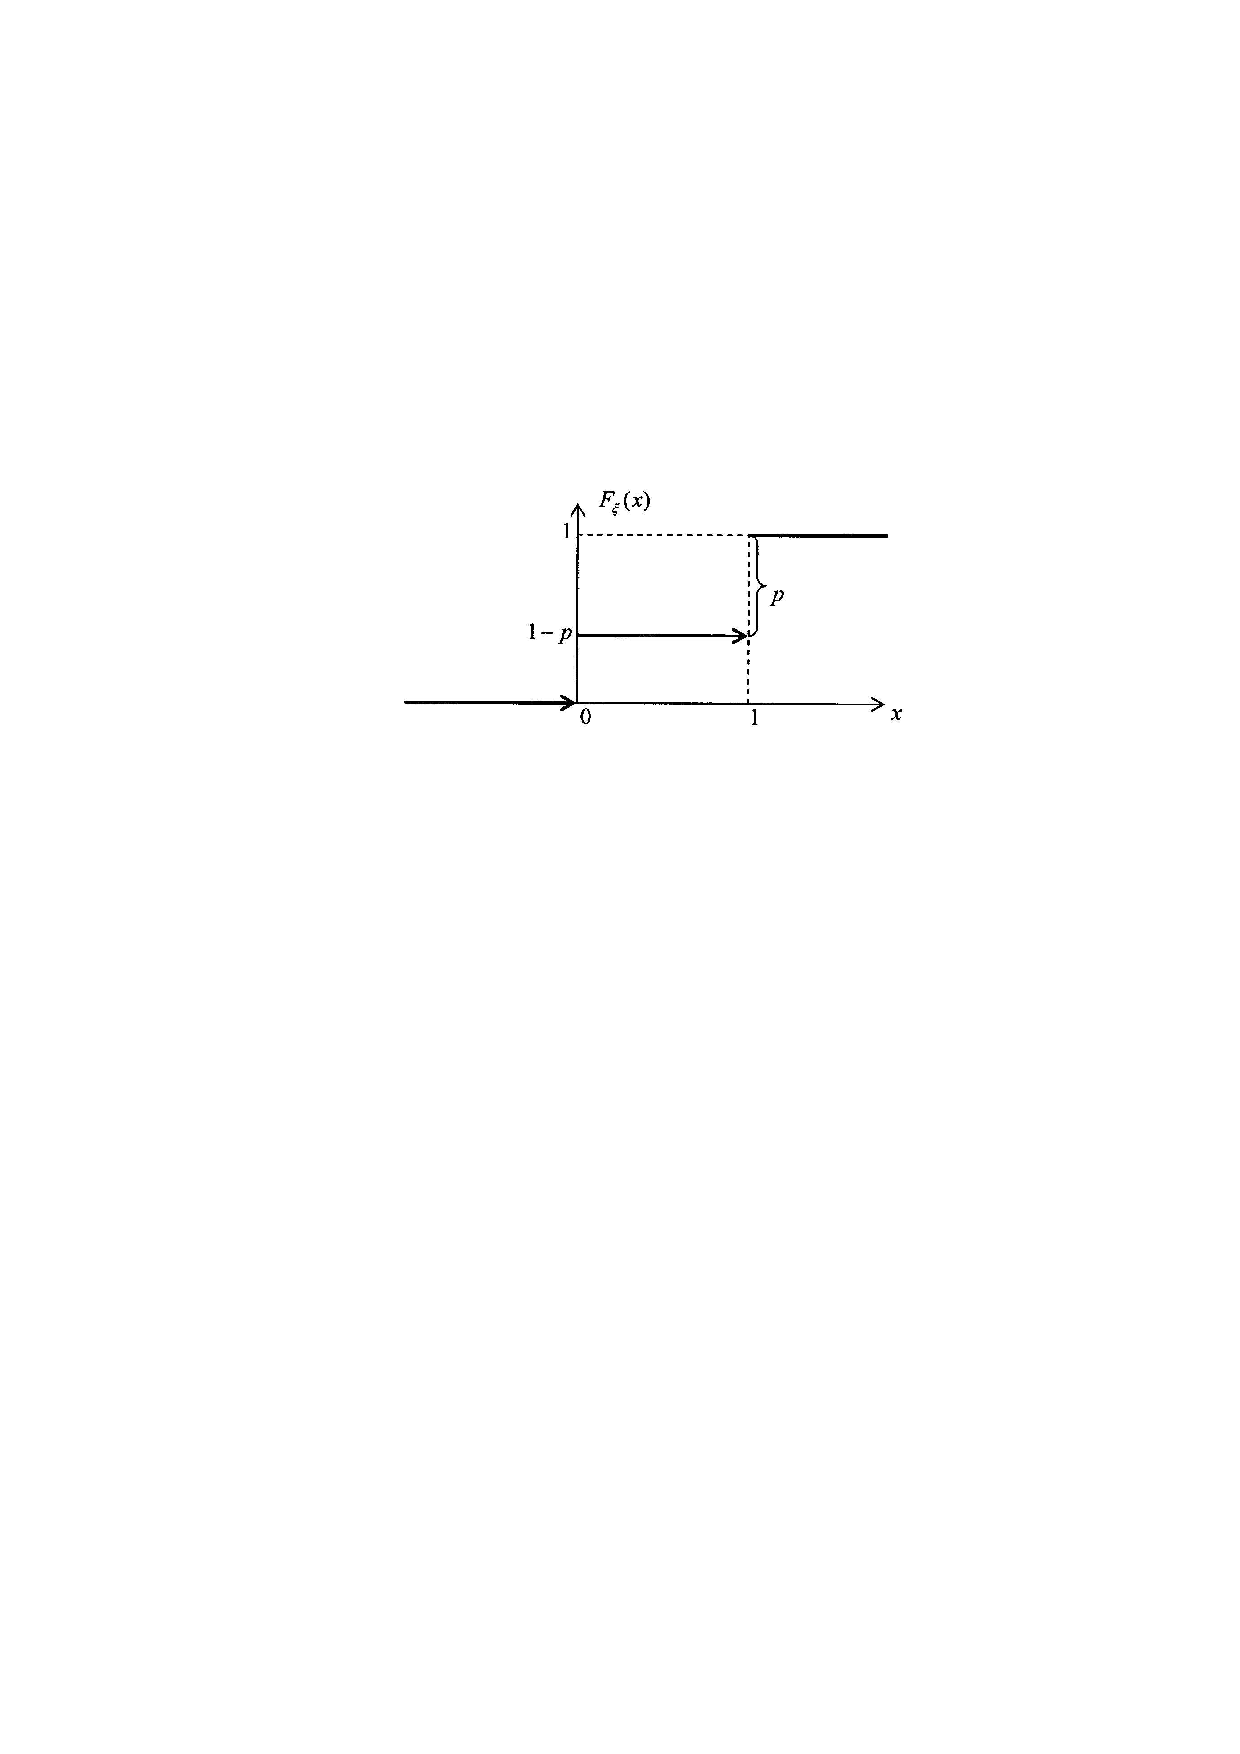
\includegraphics[]{pic/pic10}
	\caption{Функция распределения Бернулли.}
	\label{fig10}
\end{figure}

3) Случайная величина $\xi$ — номер грани при подбрасывании игральной
кости имеет функцию распределения, показанную на рис. \ref{fig11}.
\begin{figure}[H]
	\centering
	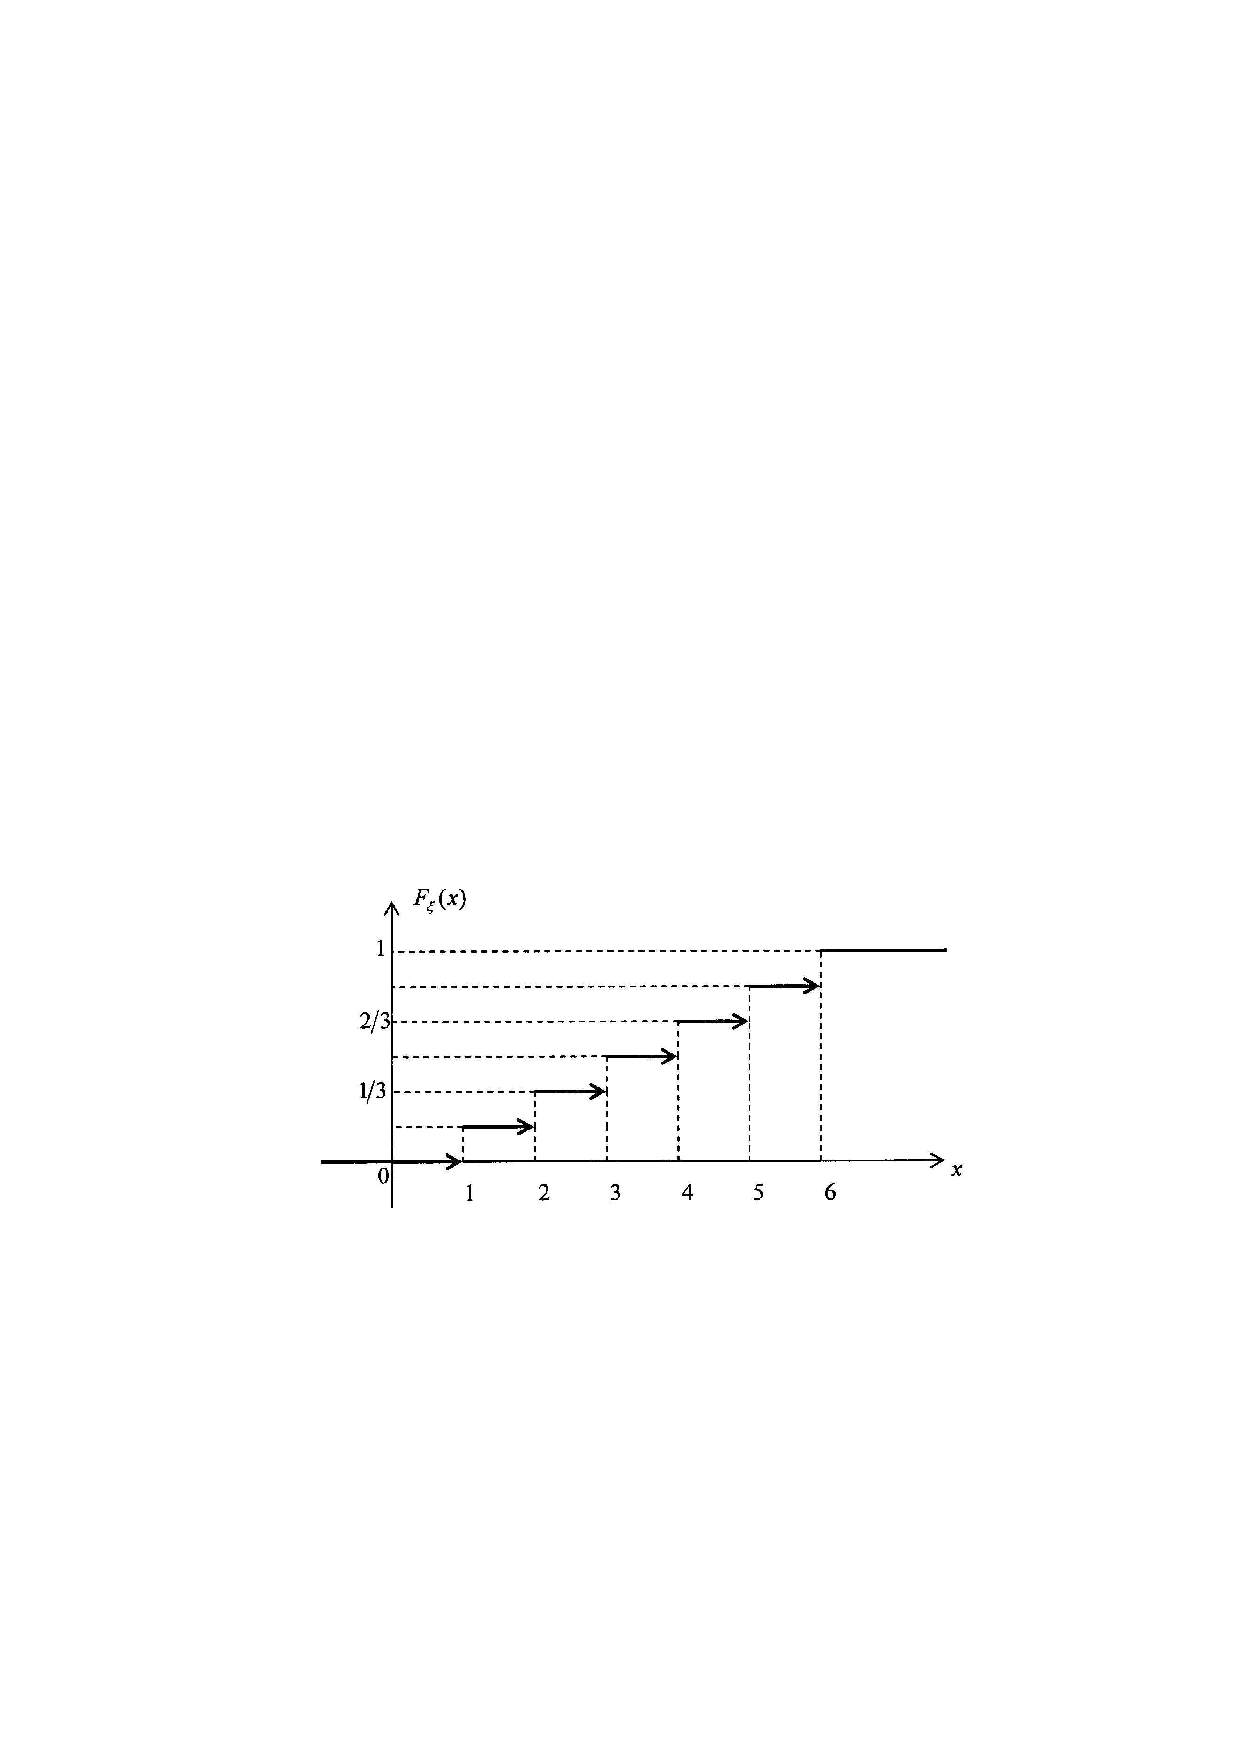
\includegraphics[]{pic/pic11}
	\caption{Функция распределения выпадения числа на игральной кости.}
	\label{fig11}
\end{figure}

4) Случайная величина $\xi$ — номер появления успеха в геометрическом
распределения имеет ряд распределения 
\begin{tabular}{|c|c|c|c|c|c|}
\hline
$\xi$ & $1$ & $2$ & $\dots$ & $k$ & $\dots$\\ \hline
$P$ & $p$ & $pq$ & $\dots$ & $pq^{k-1}$ & $\dots$\\ \hline
\end{tabular}
и имеет функцию распределения, показанную на рис. \ref{fig12}.
В дальнейшем мы будем использовать следующие обозначения для пределов функций слева и справа соответственно:
\begin{gather*}
	\lim_{\varepsilon\to 0}h(x-\epsilon)\stackrel{\text{опр}}{=}h(x-0) \,\, \text{и} \,\,
	\lim_{\varepsilon\to 0}h(x+\epsilon)\stackrel{\text{опр}}{=}h(x+0),
\end{gather*}
где всегда $\varepsilon >0$.

\begin{figure}[H]
	\centering
	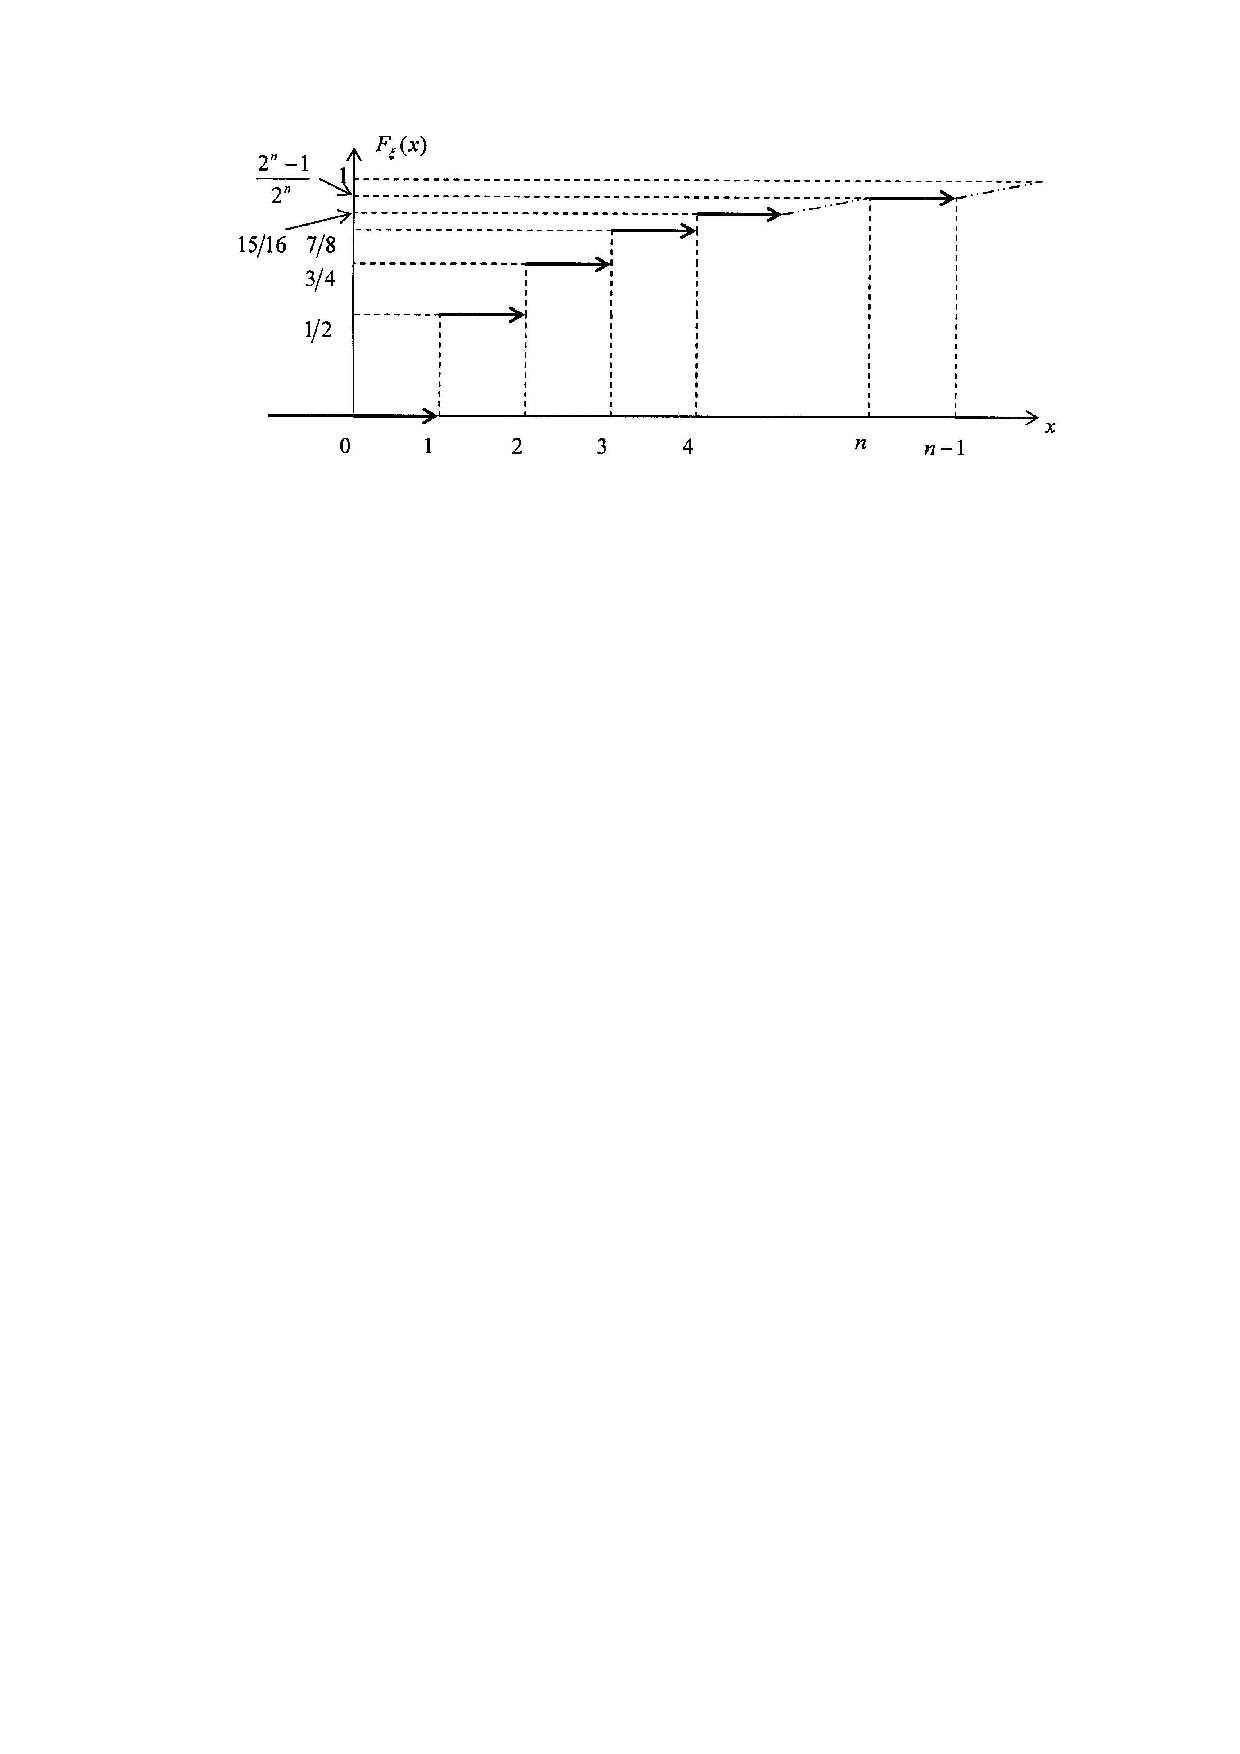
\includegraphics[]{pic/pic12}
	\caption{Функция распределения выпадения числа на игральной кости.}
	\label{fig12}
\end{figure}
\end{example}

Функция распределения $F_{\xi}(x)$ обладает следующими свойствами.

\begin{theorem}
% \newline
\vspace{1em}

	\begin{enumerate}

		\item $F_{\xi}(x)$ — неубывающая функция, другими словами,
			если $x_1 < x_2$, то $F_{\xi}(x_1) \leqslant F_{xi}(x_)$.
		\item $F_{\xi}(-\infty)=\lim\limits_{x\to-\infty}F_{\xi}(x)=0$ и 
			$F_{\xi}(+\infty)=\lim\limits_{x\to+\infty}F_{\xi}(x)=1$
		\item $F_{\xi}(x)$ непрерывна справа: для любой точки $x_0 \in \mathbb{R}$ имеем $$F_{\xi}(x+x_0) =F_{\xi}(x_0))$$
	\end{enumerate}
\end{theorem}

\begin{proof}
	По пп. \ref{def:11.3}, \ref{lemma:3.3}, 3.1 имеем  
	\begin{enumerate}
		\item $F_{\xi}(x_2)-F_{\xi}(x_1)=P(\xi\leqslant x_2)-P(\xi\leqslant x_1)=
			P\{\xi\leqslant x_2\}\ssm P\{\xi\leqslant x_1\}= \\
			=P(x_1<\xi\leqslant x_2)\geqslant 0$.
		
		\item $F_{\xi}(-\infty)=\lim\limits_{x\to-\infty}F_{\xi}(x)=\lim\limits_{x\to-\infty}P(\xi\leqslant x)=P(\xi\leqslant-\infty)=0$ \, и \,
		$F_{\xi}(+\infty)=\lim\limits_{x\to+\infty}F_{\xi}(x)=\lim\limits_{x\to+\infty}P(\xi\leqslant x)=P(\xi\leqslant+\infty)=1$.
		
		\item $F_{\xi}(x_0+0)=\lim\limits_{\varepsilon\to 0}F_{\xi}(x_0+\varepsilon)=\lim\limits_{x\to\varepsilon}P(\xi\leqslant x_0+\varepsilon)=P(\xi\leqslant x_0)=F_{\xi}(x_0)$.
		
	\end{enumerate}

\end{proof}

\begin{theorem}
	Функция распределения имеет не более чем счётное мно-
жество скачков.
\end{theorem}

\begin{proof}
	Разобьём множество H всех скачков на подмножества скач-
ков по убыванию высоты h:
	
	1) $H_1$ – множество скачков высоты $h\in(\frac{1}{2},1]$,

	2)  $H_2$ – множество скачков высоты $h\in(\frac{1}{4},\frac{1}{2}]$,

	3) $H_2$ – множество скачков высоты $h\in(\frac{1}{8},\frac{1}{4}]$,

	\dots

	$n)$ – множество скачков высоты $h\in(\frac{1}{2^n},\frac{1}{2^{n-1}}]$

	\dots



Видно, что множества $H_n$ для всех $n\in\mathbb{Z}$ попарно непересекающиеся, т.е.
$H_i \cap H_j=\O$  при $i\neq j$; и $\bigcup\limits_{i=1}^{\infty}=H$.
Функция распределения может иметь

Во-первых, 	не более одного  скачка высоты $h\in(\frac{1}{2},1]$,т.е. 
$\mu(H_1)\leqslant 1$;

Во-вторых, 	не более трёх  скачков высоты $h\in(\frac{1}{4},\frac{1}{2}]$,т.е. 
$\mu(H_2)\leqslant 3$;

В-третьих, 	не более семи  скачков высоты $h\in(\frac{1}{8},\frac{1}{4}]$,т.е. 
$\mu(H_3)\leqslant 7$;

\ldots

В-n-ых, не более $2^n-1$ скачков высоты $h\in(\frac{1}{2^n},\frac{1}{2^{n-1}}]$,т.е.
$\mu(H_n)\leqslant 2^n-1$;

\ldots

Можно занумеровать все скачки по убыванию их высоты, нумеруя при
этом скачки равной высоты, если такие повстречаются. Эта нумерация ставит
множество всех скачков во взаимно однозначное соответствие с множеством
$\mathbb{Z}$ натуральных чисел. Что и требовалось доказать.

\end{proof}

\begin{theorem}[О связи вероятности событий-интервалов с функцией
распределения.]
	Для любых точек $x,a,bin\mathbb{R}$, где $a<b$, имеем 
	\newline
	\begin{enumerate}
		\item $P(\xi<x)=F_{\xi}(x-0)$,
		\item $P(\xi=x)=F_{\xi}(x)-F_{\xi}(x-0)$,
		\item если $F_{\xi}$ непрерывна в точке x, то $P(\xi = x) = 0$;
		\item  $P(a<\xi\leqslant b)=F_{\xi}(b)-F_{\xi}(a)$,
		\item $P(a\leqslant\xi\leqslant b)=F_{\xi}(b)-F_{\xi}(a-0)$,
		\item $P(a<\xi<b)=F_{\xi}(b-0)-F_{\xi}(a)$
		\item $P(a\leqslant\xi)=F_{\xi}(b-0)-F_{\xi}(a-0)$.
	\end{enumerate}
\end{theorem}

\begin{proof}
	\begin{enumerate}
		\item $P(\xi<x)=\lim\limits_{\varepsilon\to 0} P(\xi\leqslant x-\varepsilon)=
		\lim\limits_{\varepsilon\to 0} F_{\xi}(x-\varepsilon)=F_{\xi}(x-0)$.

		\item $P(\xi=x)=P(\{\xi\leqslant x\})\ssm\{\xi<x \})=P(\xi\leqslant x)-P(\xi<x)=F_{\xi}(x)-F_{\xi}(x)$.

		\item $P(\xi=x)=F_{\xi}-F_{\xi}(x-0)=F_{\xi}(x)-\lim\limits_{\varepsilon\to 0} F_{\xi}(x-\varepsilon)=F_{\xi}(x)-F_{\xi}(x)=0.$

		\item $P(a<\xi\leqslant b)= P(\{\xi\leqslant b \})\ssm \{\xi\leqslant a \}=
		P(\xi\leqslant b)-P(\xi\leqslant a)= F_{\xi}(b)-F_{\xi}(a).$

		\item Самостоятельно

		\item Самостоятельно

		\item Самостоятельно
	\end{enumerate}
\end{proof}

\begin{consq}
	Если функция распределения $F_{\xi}(x)$ непрерывна, то 
	\begin{gather*}
		P(a\leqslant \xi<b)=P(a<\xi<b)=P(a\leqslant \xi \leqslant b)= P(a< \xi\leqslant b)= \\ 
		=P(a<\xi\leqslant b)=F_{\xi}(b)-F_{\xi}(a).
	\end{gather*}
\end{consq}% кирилл

\section{Абсолютно непрерывные случайные величины}
%!TEX root = ../var.tex
\begin{definition}
\label{def:12.1}
	Случайная величина $\xi$ называется абсолютно непрерывной, если существует такая неотрицательная функция $f_{\xi} (x)$ (возможно обобщённая, см. §13), что для любого $x \in \mathbb{R}$ функция распределения $F_{\xi}(x)$ представима в виде\footnote{В дальнейшем мы рассматриваем только такие случайные величины, для которых все связанные с
ними несобственные интегралы и суммы бесконечных рядов сходятся абсолютно.
	}
  
\begin{equation*}
	F_{\xi}(x)=\int_{-\infty}^{x} f_{\xi}(t) dt  	
\end{equation*}

При этом функция $f_{\xi}(x)$ называется плотностью вероятности случайной величины $\xi$
\end{definition}

\begin{zam}
\label{zam:12.2}
Если $F_{\xi}(x)$ -- дифференцируемая функция распределения, то название <<плотность вероятности>> имеет следующее объяснение. С одной стороны, используя формулу дифференцирования интеграла по верхнему пределу, имеем $\frac{dF_{\xi}(x)}{dx}=f_{\xi}(t)|_t=x$. С другой стороны, по определению производной имеем:

\begin{gather*}
	\frac{dF_{\xi}(x)}{dx} = \frac{F_{\xi}(x+dx)-F_{\xi}(x)}{dx}=\frac{\P(\xi \leq x+dx)-\P(\xi \leq x)}{dx}=\\=\frac{\P(\{\xi \leq x+dx \}\ssm \{\xi \leq x\})}{dx} = \frac{\P(x<\xi \leq x+dx)}{dx}
\end{gather*}
Поэтому

\begin{equation*}
	f_{\xi}(x)=\frac{\P(x,\xi \leq x+dx)}{dx}	 
\end{equation*}
есть отношение вероятности попадания случайной величины $\xi$ в интервал $(x, x+dx]$ к длине этого интервала $dx$, что физически означает плотность вероятности (<<массы>>) случайной величины $\xi$ в точке $x$.
\end{zam}
 

 \begin{theorem}
 \label{th:12.3}
Плотность обладает свойствами:

1) $f_{\xi}(x) \geq 0$ для любого $x$;

2) $\int\limits_{-\infty}^{\infty} f_{\xi}(t)dt=1$
 \end{theorem}

\begin{proof}

1) По теор. 11.4.1 функция распределения $F_{\xi}(x)$ -- неубывающая, поэтому $\frac{dF_{\xi}(x)}{dx}=f_{\xi}(x) \geq 0$

2) $\int\limits_{-\infty}^{\infty}f_{\xi}(t)dt = \lim\limits_{x \to \infty}\int\limits_{-\infty}^{x}f_{\xi}(t)dt = \lim\limits_{x \to \infty}F_{\xi}(x) = 1$ по свойству 11.4.2.
\end{proof} 

\begin{definition}
 \label{def:12.4}

Пусть область $U \subseteq \mathbb{R}^n$ имеет меру $\mu(U )$. Говорят, что в области $U$ функция $h : U \to \mathbb{R}$ удовлетворяет некоторому свойству $\mathcal{P}$ почти всюду, если подмножество $A \subset U$ , в котором свойство $\mathcal{P}$ не выполняется, имеет меру 0, т.е. $\mu(A) = 0$.
Докажем свойства абсолютно непрерывных случайных величин.
\end{definition}

\begin{theorem}
 \label{th:12.5}

Если случайная величина $\xi$ абсолютно непрерывна, то

1) её функция распределения $F_{\xi}(x)$ непрерывна в $\mathbb{R}$ и дифференцируема почти всюду в $\mathbb{R}$, т.е. равенство $f_{\xi}(x) = \frac{d}{dx}F_{\xi}(x)$ справедливо почти всюду,

2) $\P(\xi = x) = 0$ для любого $x \in \mathbb{R}$,

3) $\P(a \leq \xi < b) = \P(a < \xi < b) = \P(a \leq \xi \leq b) = \P(a < \xi \leq b) = \int_{a}^{b}f_{\xi}(t)dt.$
\end{theorem}

\begin{proof}
1) Во-первых, функция $F_{\xi}(x) = \int_{-\infty}^{x}f_{\xi}(t)dt$ непрерывна как функция верхнего предела интеграла.
Во-вторых, по теор. \ref{th:11.5} функция $F_{\xi}(x)$ имеет не более чем счётное множество скачков, поэтому она не дифференцируема не более чем в счётном
множестве точек. Любое счётное множество точек на прямой имеет нулевую меру (длину). Поэтому $F_{\xi}(x)$ дифференцируема почти всюду в $\mathbb{R}$.

2) Это следует из \ref{th:11.6}.3).

3) Из \ref{th:11.6}.4) имеем
$$\P(a < \xi \leq b) = F_{\xi}(b) - F_{\xi}(a) = \int\limits_{-\infty}^{b}f_{\xi}(t)dt - \int\limits_{-\infty}^{a}f_{\xi}(t)dt = \int\limits_{a}^{b}f_{\xi}(t)dt$$

\end{proof}
Остальные равенства следуют из \ref{consq:11.7}.

\vspace{1em}\textbf{Примеры абсолютно непрерывных случайных величин}

\begin{definition}
 \label{def:12.6}

Случайная величина $\xi$ имеет равномерное распределение на отрезке $a, b$, если

\begin{equation*}
	F_{\xi}(x) = \P(\xi \leq x) = 
	\left\{
	\begin{aligned}
		&0, & x<a\\
		&\frac{x-a}{b-a}, & a \leq x \leq b\\
		&1, & x>b\\
	\end{aligned}\right. \text{   и } f_{\xi}(x) = 
	\left\{
	\begin{aligned}
		&0, & x<a\\
		&\frac{1}{b-a}, & a \leq x \leq b\\
		&1, & x>b\\
	\end{aligned}\right.
\end{equation*}

Графики функций $F_{\xi}(x)$ и $f_{\xi}(x)$ показаны на рис. 13. Заметим, что в точках $a$ и $b$ функция распределения $F_{\xi}(x)$ не дифференцируема, поэтому значение плотности вероятности в этих точках можно задать как угодно: либо $f_{\xi}(a) = 0$, либо $f_{\xi}(a) = \frac{1}{b-a}$, а на другом конце тоже либо $f_{\xi}(b) = 0$, либо $f_{\xi}(b) = \frac{1}{b-a}$
\end{definition}
	
\begin{definition}
 \label{def:12.7}
Случайная величина $\xi$ имеет показательное распределение с параметром $\lambda$ (рис. 14), если

\begin{equation*}
	f_{\xi}(x) = 
	\left\{
	\begin{aligned}
		&0, & x<0\\
		&\lambda e^{-\lambda x}, & x \geq 0\\
	\end{aligned}\right.
\end{equation*}
\end{definition}

\begin{figure}[H]
	\centering
	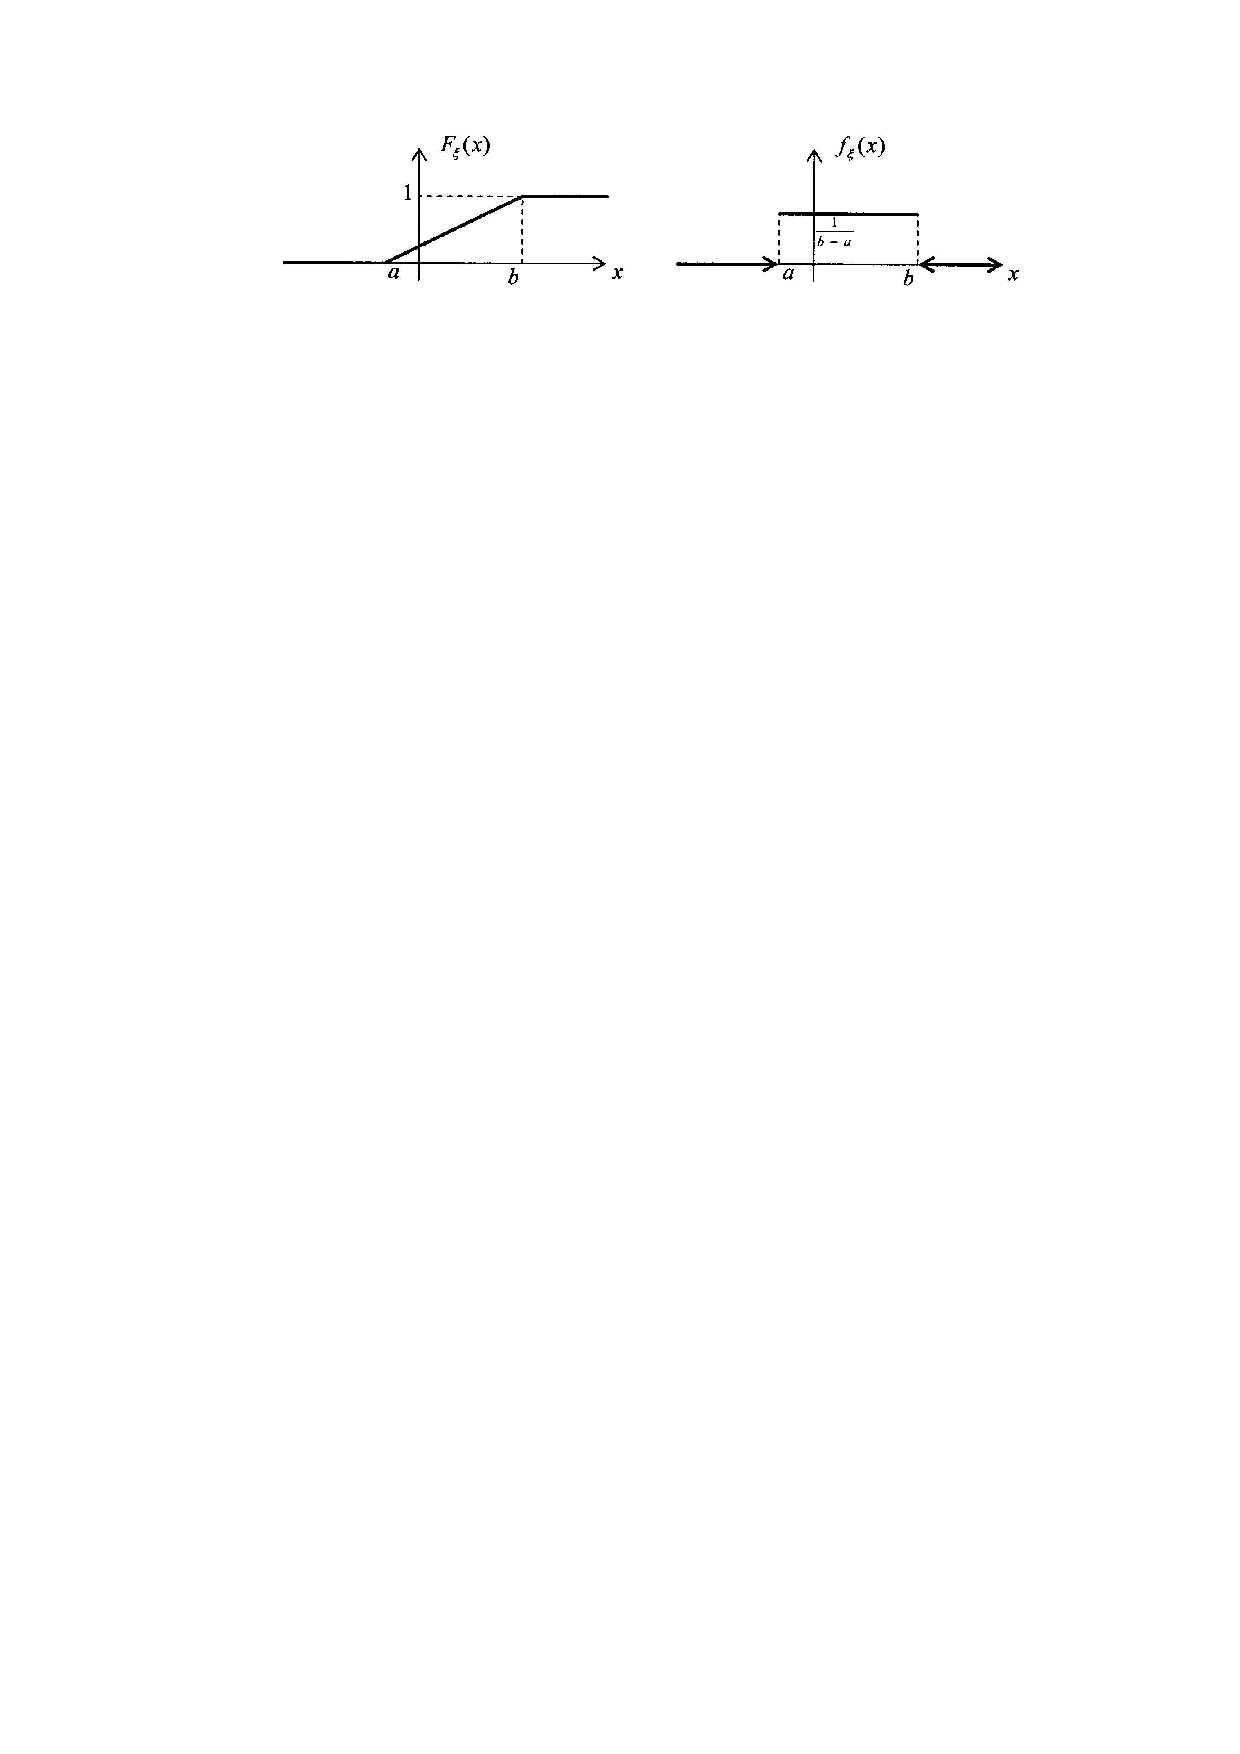
\includegraphics[]{pic/pic13}
	\caption{Равномерное распределение}
	\label{fig13}
\end{figure}
\begin{figure}[H]
	\centering
	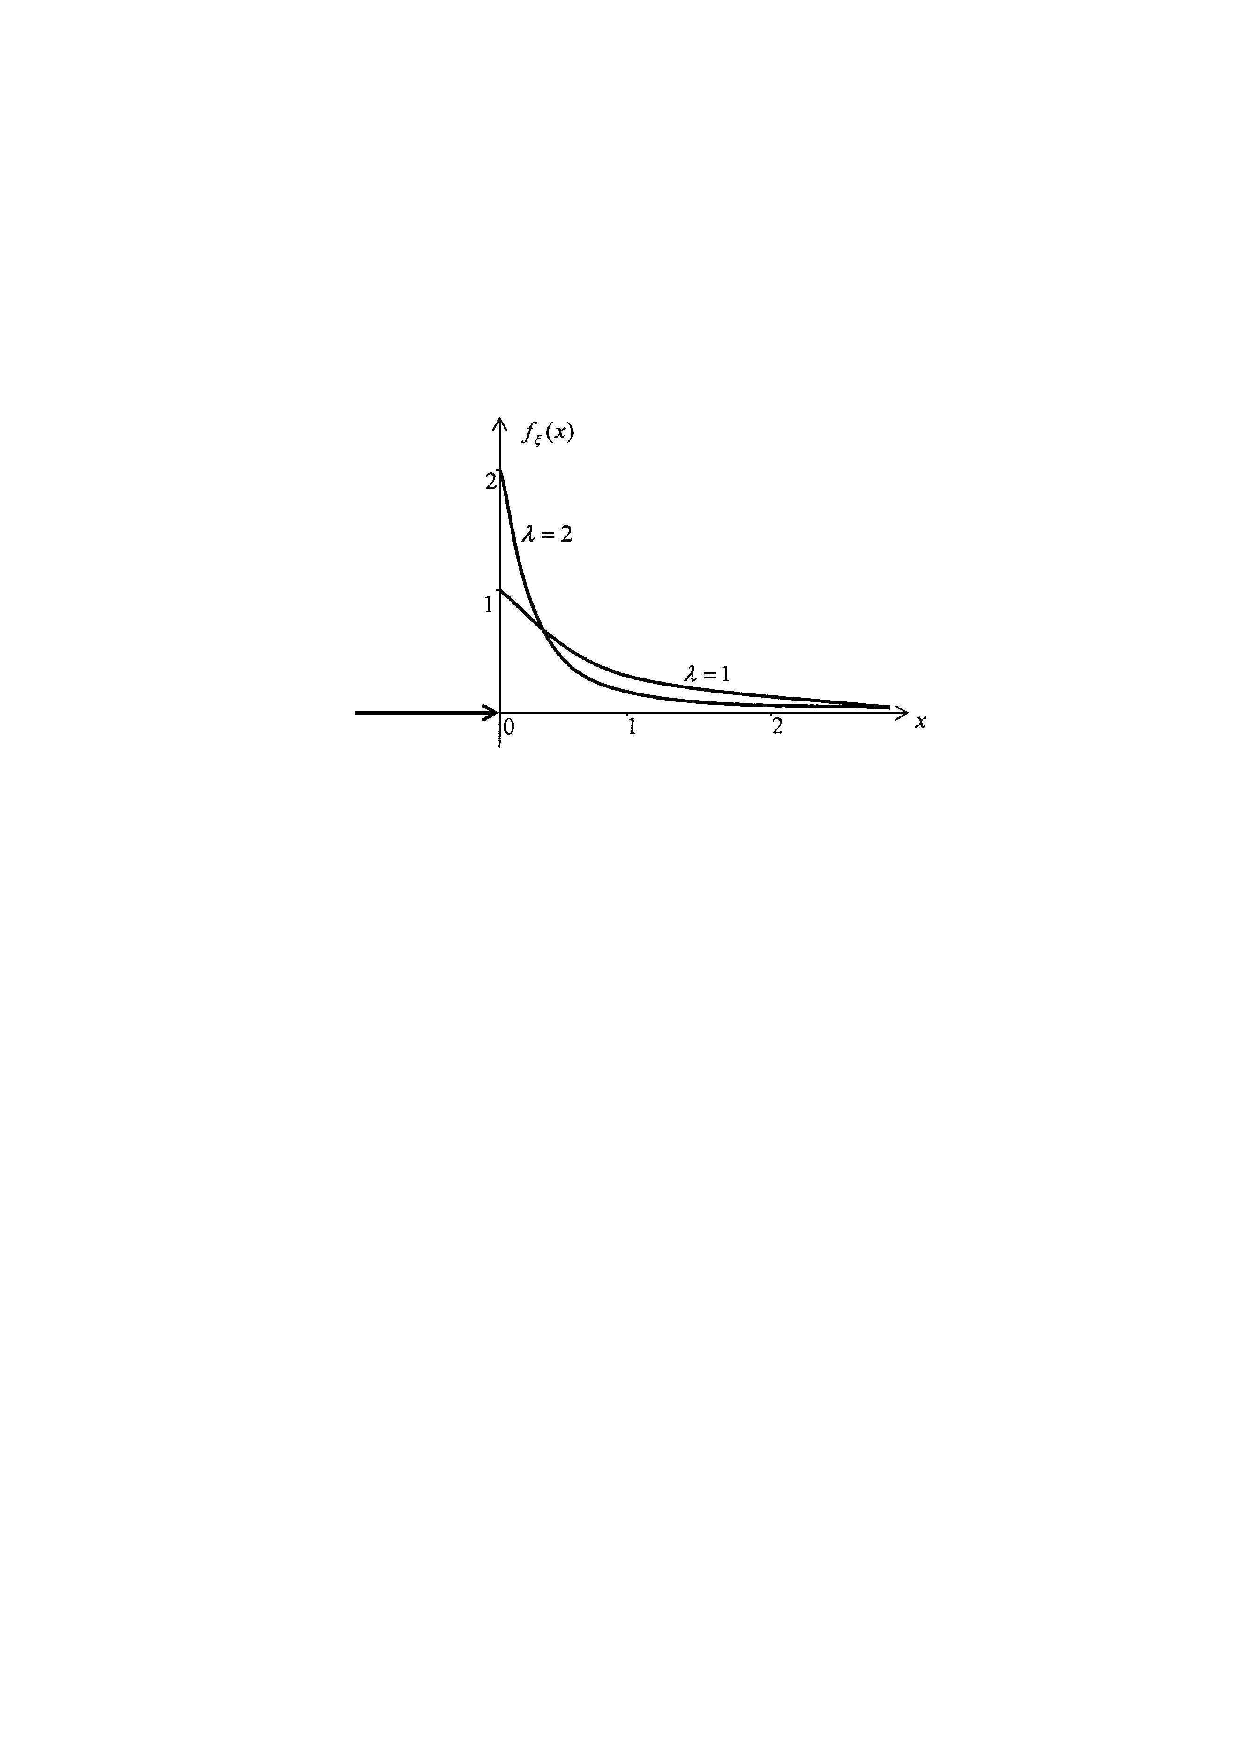
\includegraphics[]{pic/pic14}
	\caption{Показательное распределение}
	\label{fig14}
\end{figure}

\begin{definition}
 \label{def:12.8}
Если для любого $x \in \mathbb{R}$ случайная величина $\xi$ имеет плотность
\begin{equation*}
	f_{\xi}(x) = \frac{1}{2 \sqrt{2\pi}}e^{-\frac{(x-a)^2}{2\sigma^2}},
\end{equation*}

то говорят, что $\xi$ имеет нормальное (или Гаусса\footnote{
Карл Фридрих Гаусс (Johann Carl Friedrich Gauß, 1777 — 1855), выдающийся немецкий математик,
астроном и физик, считается одним из величайших математиков всех времён.	
} 
) распределение с математическим ожиданием $a$ и дисперсией $\sigma^2$ , где $a \in \mathbb{R}$ и $\sigma > 0$. (См. рис. 15) Очевидно, что $f_{\xi}(x) \geq 0$ для любого $x$;

2) Используем табличный интеграл (Пуассона)
$\int_{-\infty}^{\infty}e^{-\frac{t^2}{2}}dt=\sqrt{2\pi}$.

\begin{gather*}
	\int_{-\infty}^{\infty} f_{\xi}(x)dx = \int_{-\infty}^{\infty} \frac{1}{\sigma \sqrt{2\pi}}e^{-\frac{(x-a)^2}{2\sigma^2}}dx =
	%
	\left[
	\begin{aligned}
		\text{замена переменных}\\
		t = \frac{x-a}{\sigma}, dx = \sigma dt
	\end{aligned}\right]=\\=
	\frac{1}{\sqrt{2\pi}}\int_{-\infty}^{\infty}e^{-\frac{t^2}{2}}dt=1.
\end{gather*}
\end{definition}

\begin{prop}
 \label{prop:12.9}
 Легко сосчитать, что расстояние между точками перегиба равно $2\sigma$, поэтому параметр $2\sigma$ является характеристикой ширины графика на уровне точек перегиба.

\begin{figure}[H]
	\centering
	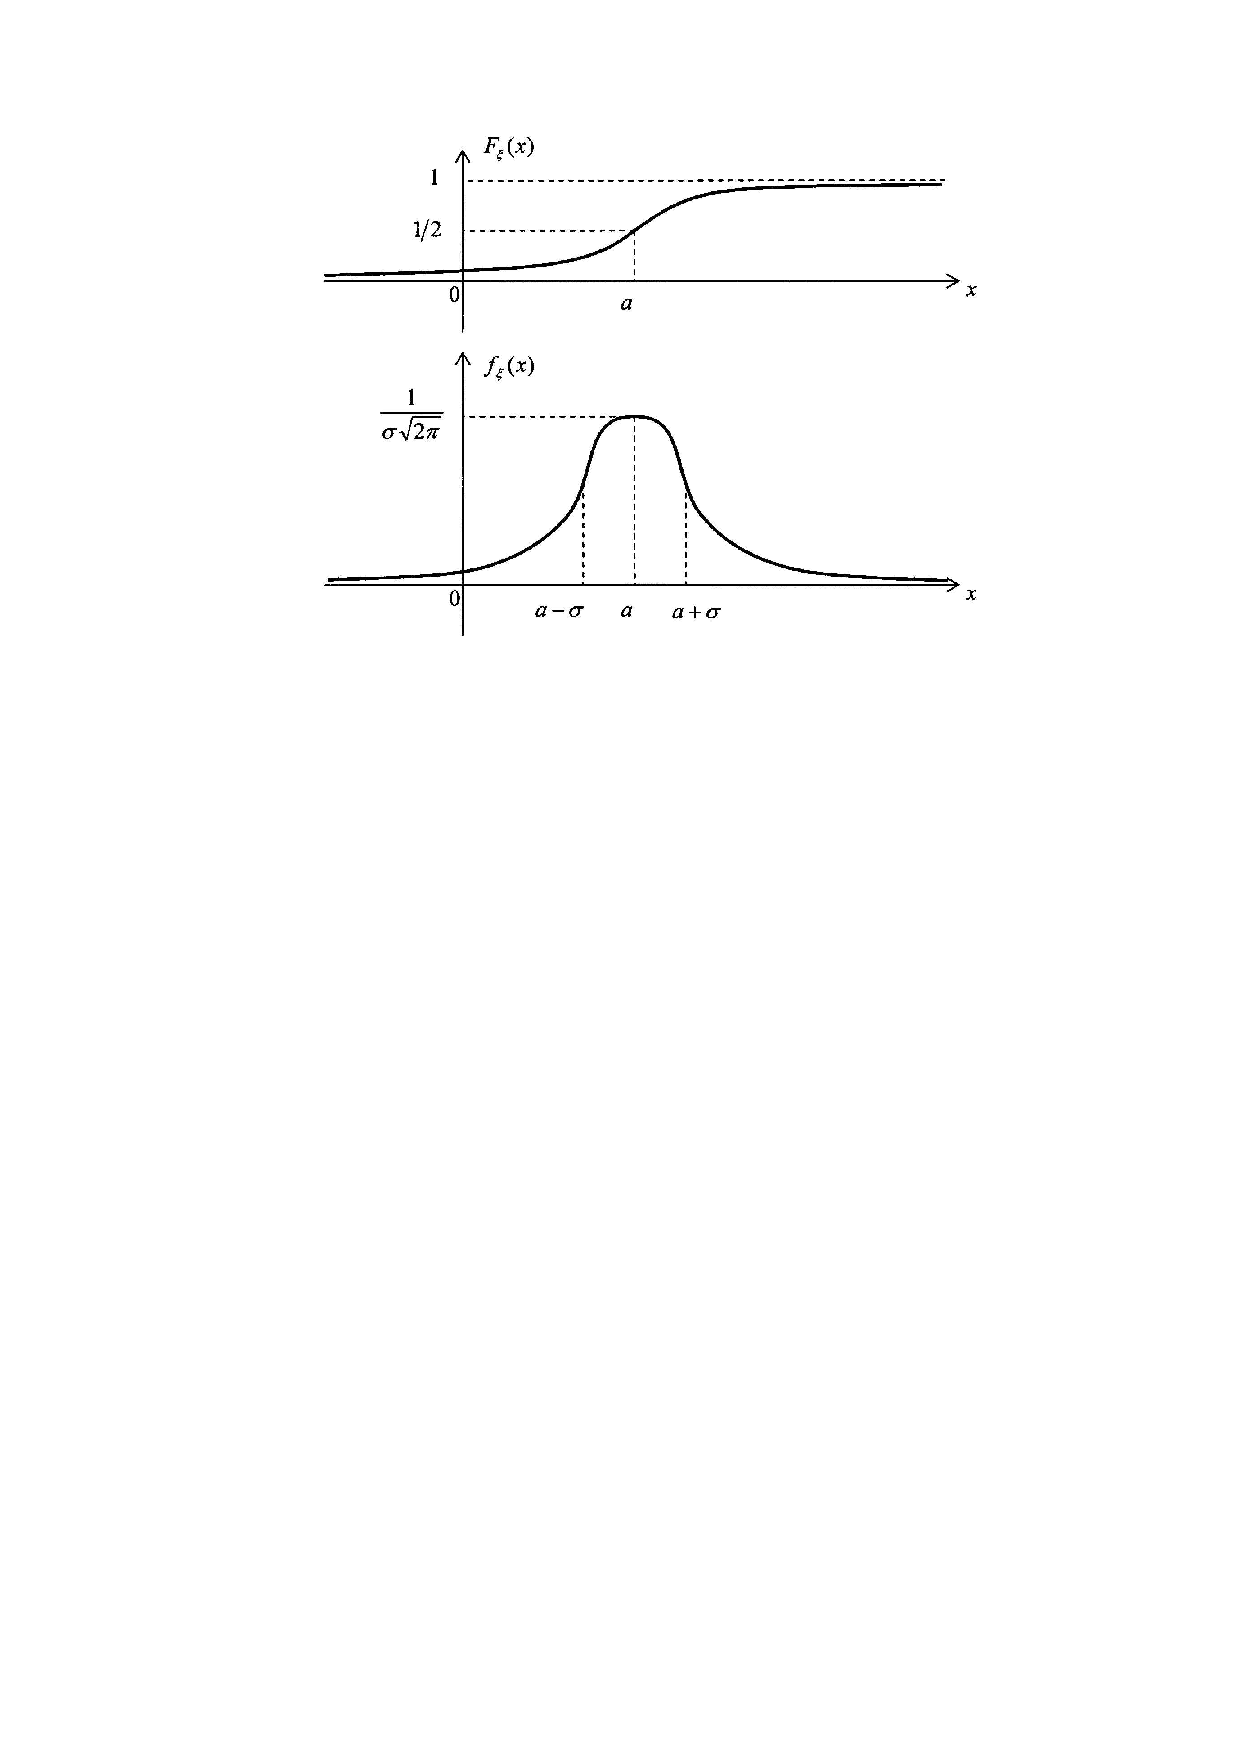
\includegraphics[]{pic/pic15}
	\caption{Нормальное распределение (Гаусса)}
	\label{fig15}
\end{figure}
 Заметим, что вероятность попадания  нормальной случайной величины в интервал между точками перегиба
\begin{equation*}
	\P(a − \sigma \leq \xi \leq a + \sigma) = \frac{1}{\sigma \sqrt{2\pi}} \int\limits_{a-\sigma}^{a+\sigma} e^{-\frac{(x-a)^2}{2\sigma^2}}dx =  \frac{1}{\sigma \sqrt{2\pi}} \int\limits_{-1}^{1} e^{-\frac{t^2}{2}}dt = 2\Phi(1) \approx 0.6827
\end{equation*}

где $\Phi(1)$ приближённое значение функции $\Phi (x) = \frac{1}{\sqrt{2\pi}} \int_{0}^{x}e^{-\frac{t^2}{2}}dt$
взято из таблицы.
\end{prop}

\begin{prop}[<<Правило трёх сигм>>]
 \label{prop:12.10}
Если $\xi$ — нормальная случайная величина, то $\P(|\xi − a| \leq 3\sigma) = 2\Phi(3) \approx 2\cdot0.49865 \approx 0,997$. Запоминать число $0,997$ нет никакого смысла, а вот помнить, что почти вся вероятность (<<масса>>) нормального распределения сосредоточена в интервале $[a − 3\sigma, a + 3\sigma]$, всегда полезно.
\end{prop}
 %Рита

\section{Функции Хевисайда и Дирака}
%!TEX root = ../var.tex
\begin{theorem}
\label{th:13.1}
	Функцией единичного скачка или короче функцией
Хевисайда\footnote{Оливер Хевисайд (англ. Oliver Heaviside; 18 мая 1850 — 3 февраля 1925) — английский учёный-
самоучка, инженер, математик и физик. Впервые применил комплексные числа для изучения электрических цепей. Переписал уравнения Максвелла из их первоначальной формы, состоявшей из 20 уравнений
с 12 переменными, к современной форме, состоящей из 4 дифференциальных уравнений, выраженной в
терминах современного векторного анализа. Предложил операционное исчисление (он ввёл обозначение D
для дифференциального оператора) и метод решения дифференциальных уравнений с помощью сведения
к обыкновенным алгебраическим уравнениям. Ввёл термины: «проводимость», «проницаемость», «индуктивность», «импеданс».} называется функция $U : \mathbb{R}\rightarrow \mathbb{R}$, заданная по формуле (см. рис. \ref{fig16})

\begin{equation*}
u(x) = 
 \left\{\begin{aligned}
   0,x<0\\
   1,x\geqslant 0 
 \end{aligned}\right\}
\end{equation*}
\end{theorem}

\begin{figure}[H]
	\centering
	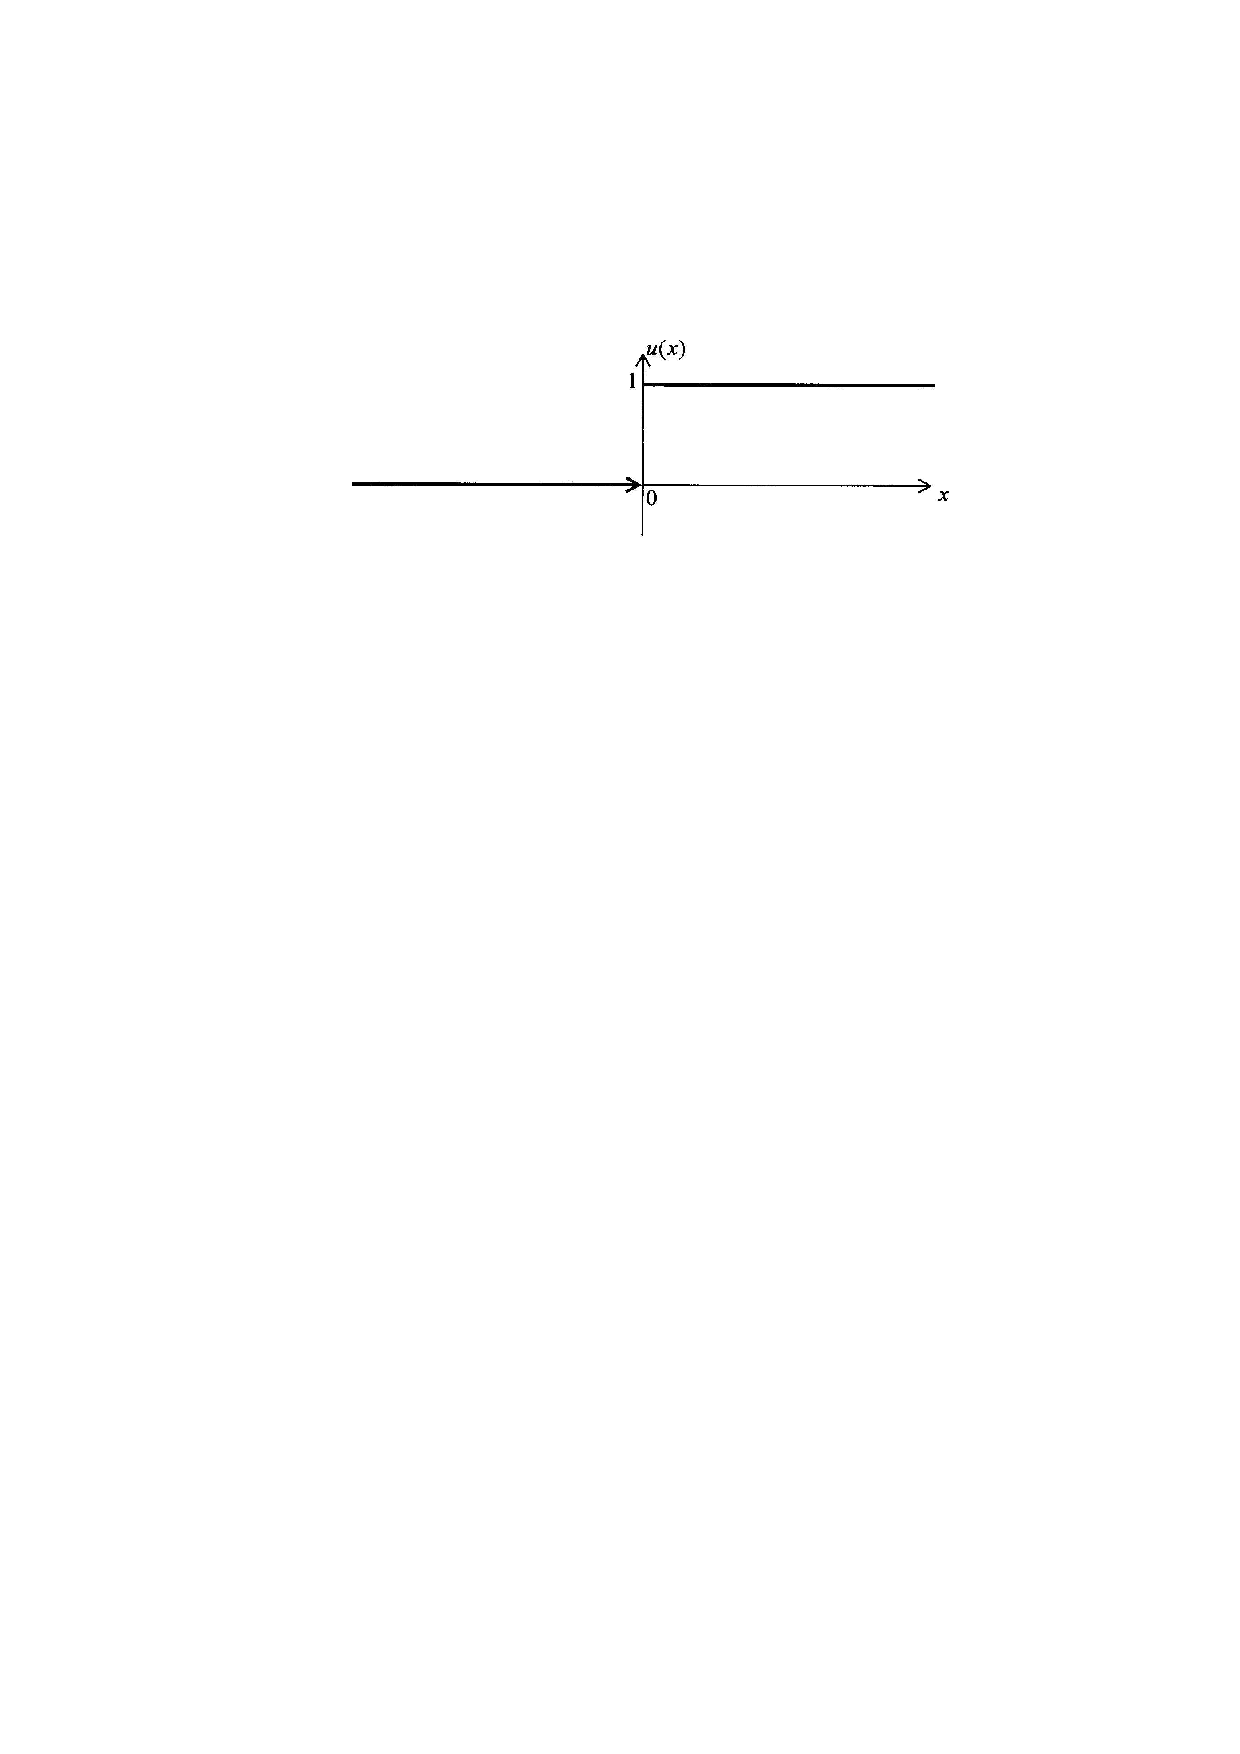
\includegraphics[]{pic/pic16}
	\caption{Функция Хевисайда}
	\label{fig16}
\end{figure}

\begin{example}
\label{ex:13.2}

	Функция Хевисайда полезна для записи в строчку формул (многоэтажных) кусочно заданных функций.

1) Функция единичного импульса единичной длины см. рис. \ref{fig17}.
\begin{equation*}
U(x) = \left\{
 \begin{aligned}
   &0,&x<0\\
   &1,&x\geqslant 0\\
   &0,&x>1
 \end{aligned}\right\}
 =u(x)-u(x-1).
\end{equation*}

\begin{figure}[H]
	\centering
	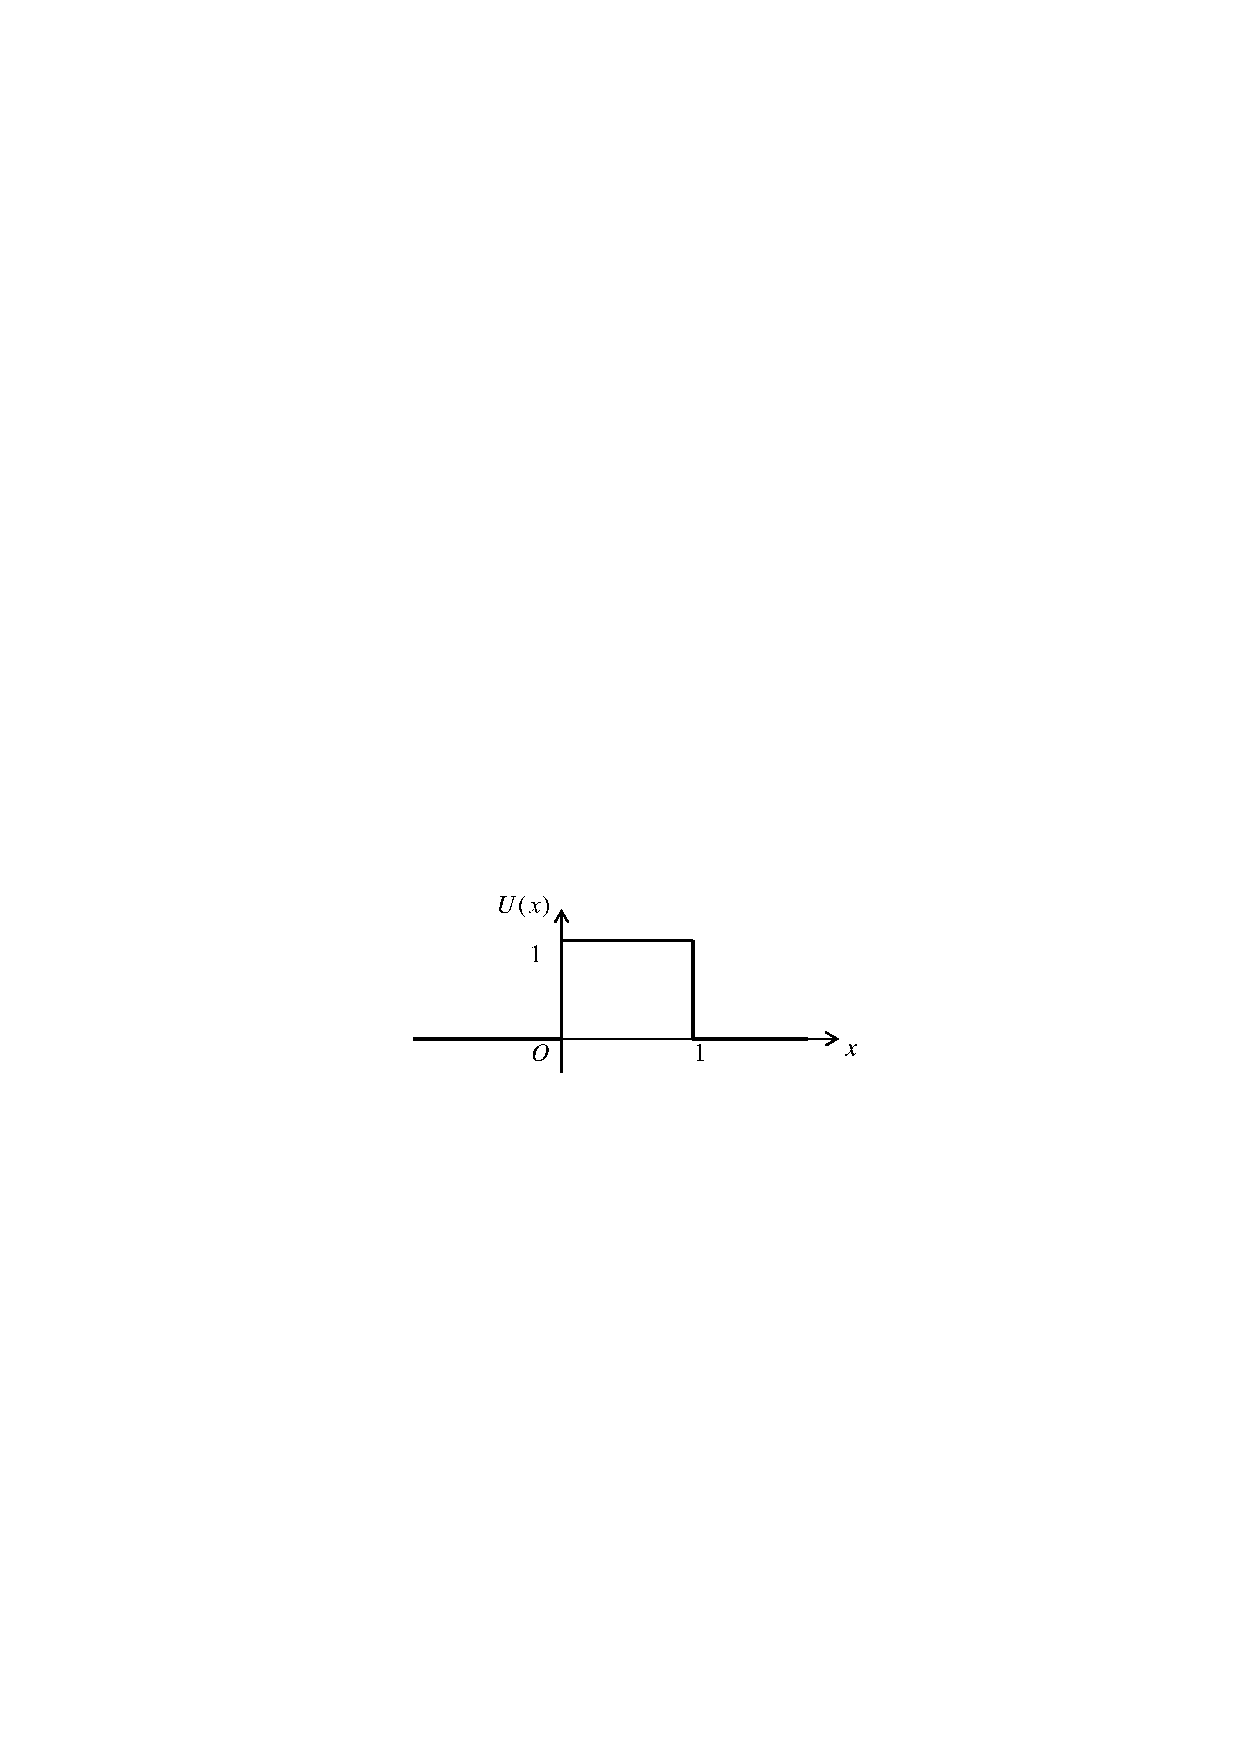
\includegraphics[]{pic/pic17}
	\caption{$U(x) = u(x)-u(x-1)$}
	\label{fig17}
\end{figure}

2) Функция распределения Бернулли, см. рис. \ref{fig10}.
\begin{equation*}
F_{\xi}(x) = 
  \left\{
 \begin{aligned}
   &0,&x<c\\
   &1-p,&0\leqslant x<1\\
   &p,&1\leqslant x
 \end{aligned}\right\}
 =(1-p)u(x)-pu(x-1).
\end{equation*}

3) Функция равномерного распределения, см. рис. \ref{fig13}
\begin{equation*}
F_{\xi}(x) = 
 \left\{\begin{aligned}
   &0,	&x<a\\
   &\frac{x-a}{b-a},	&a\leqslant x<b\\
   &1,	&x\geqslant b
 \end{aligned}\right\}
 =
 \frac{x-a}{b-a}u(x-a)-\frac{x-a}{b-a}u(x-b)+u(x-b).
\end{equation*}

4) Интеграл от функции Хевисайда.
\begin{equation*}
	\int\limits_{-\infty}^x f(t)u(t)dt=\int\limits_0^xf(t)dt
\end{equation*}
в частности,
\begin{equation*}
	\int\limits_{-\infty}^x u(t)dt=xu(x).
\end{equation*}

\end{example}

\begin{lemma}
\label{lemma:13.3}
	Кусочная функция
\begin{equation*}
	g(x)=
	\left\{\begin{aligned}
		&g_0(x),	&x<x_0 \\
		&g_1(x), 	&x_0\leqslant x<x_1\\
		&\ldots,	&\ldots\\
		&g_n(x),	&x_{n-1}\leqslant x<x_n\\
		&g_{n+1}(x), &x_n\leqslant x
 	\end{aligned}\right.
\end{equation*}
	представима в виде

\begin{gather*}
g(x)=g_0(x)u(x_0-x)+g_1(x)[u(x-x_0)-u(x-x_1)]+\ldots \\
\ldots+g_n(x)[u(x-x_{n-1})-u(x-x_n)]+g_{n+1}(x)u(x-x_n).
\end{gather*}
\end{lemma}

\begin{proof}
	Функция $g(x)$ является суммой следующих функций
	\begin{equation*}
		\widetilde{g}_0(x)=
		\left\{\begin{aligned}
			&g_0(x), &x<x_0\\
			&0,		&x_0\leqslant x
		\end{aligned}\right\}
		=g_0(x)u(x_0-x),
	\end{equation*}

	\begin{equation*}
		\widetilde{g}_1(x)=
		\left\{\begin{aligned}
			&0(x), &x<x_0 \text{ или } x_1\leqslant x \\
			&g_1(x), &x_0\leqslant x<x_1
		\end{aligned}\right\}
		=g_1(x)u(x-x_0)-g_1(x)u(x-x_1),
	\end{equation*}

	\begin{equation*}
		\widetilde{g}_n(x)=
		\left\{\begin{aligned}
			&0(x), &x<x_{n-1} \text{ или } x_n\leqslant x \\
			&g_n(x), &x_{n-1}\leqslant x<x_n
		\end{aligned}\right\}
		=g_n(x)u(x-x_{n-1})-g_n(x)u(x-x_{n-n}),
	\end{equation*}

		\begin{equation*}
		\widetilde{g}_{n+1}(x)=
		\left\{\begin{aligned}
			&0(x), &x<x_{n}\\
			&g_n(x),&x_{n}\leqslant x<x_n
		\end{aligned}\right\}
		=g_0(x)u(x-x_{n}).
	\end{equation*}

\end{proof}

\begin{definition}
\label{def:13.4}
	$\delta$-функцией или функцией Дирака называется обобщённая функция
	$\delta : \mathbb{R}\rightarrow\mathbb{R}\cup\{\infty\}$, заданная по формуле

	\begin{equation*}
		\delta(x)=
		\left\{\begin{aligned}
			&0, &x \neq 0 \\
			&\infty, &x=0			
		\end{aligned}\right.
	\end{equation*}
	и для любого $\varepsilon > 0$ подчинённая условию $\int\limits^\varepsilon_{-\varepsilon}\delta(x)dx=1$. См. рис. \ref{fig18}.
\end{definition}

\begin{figure}[H]
	\centering
	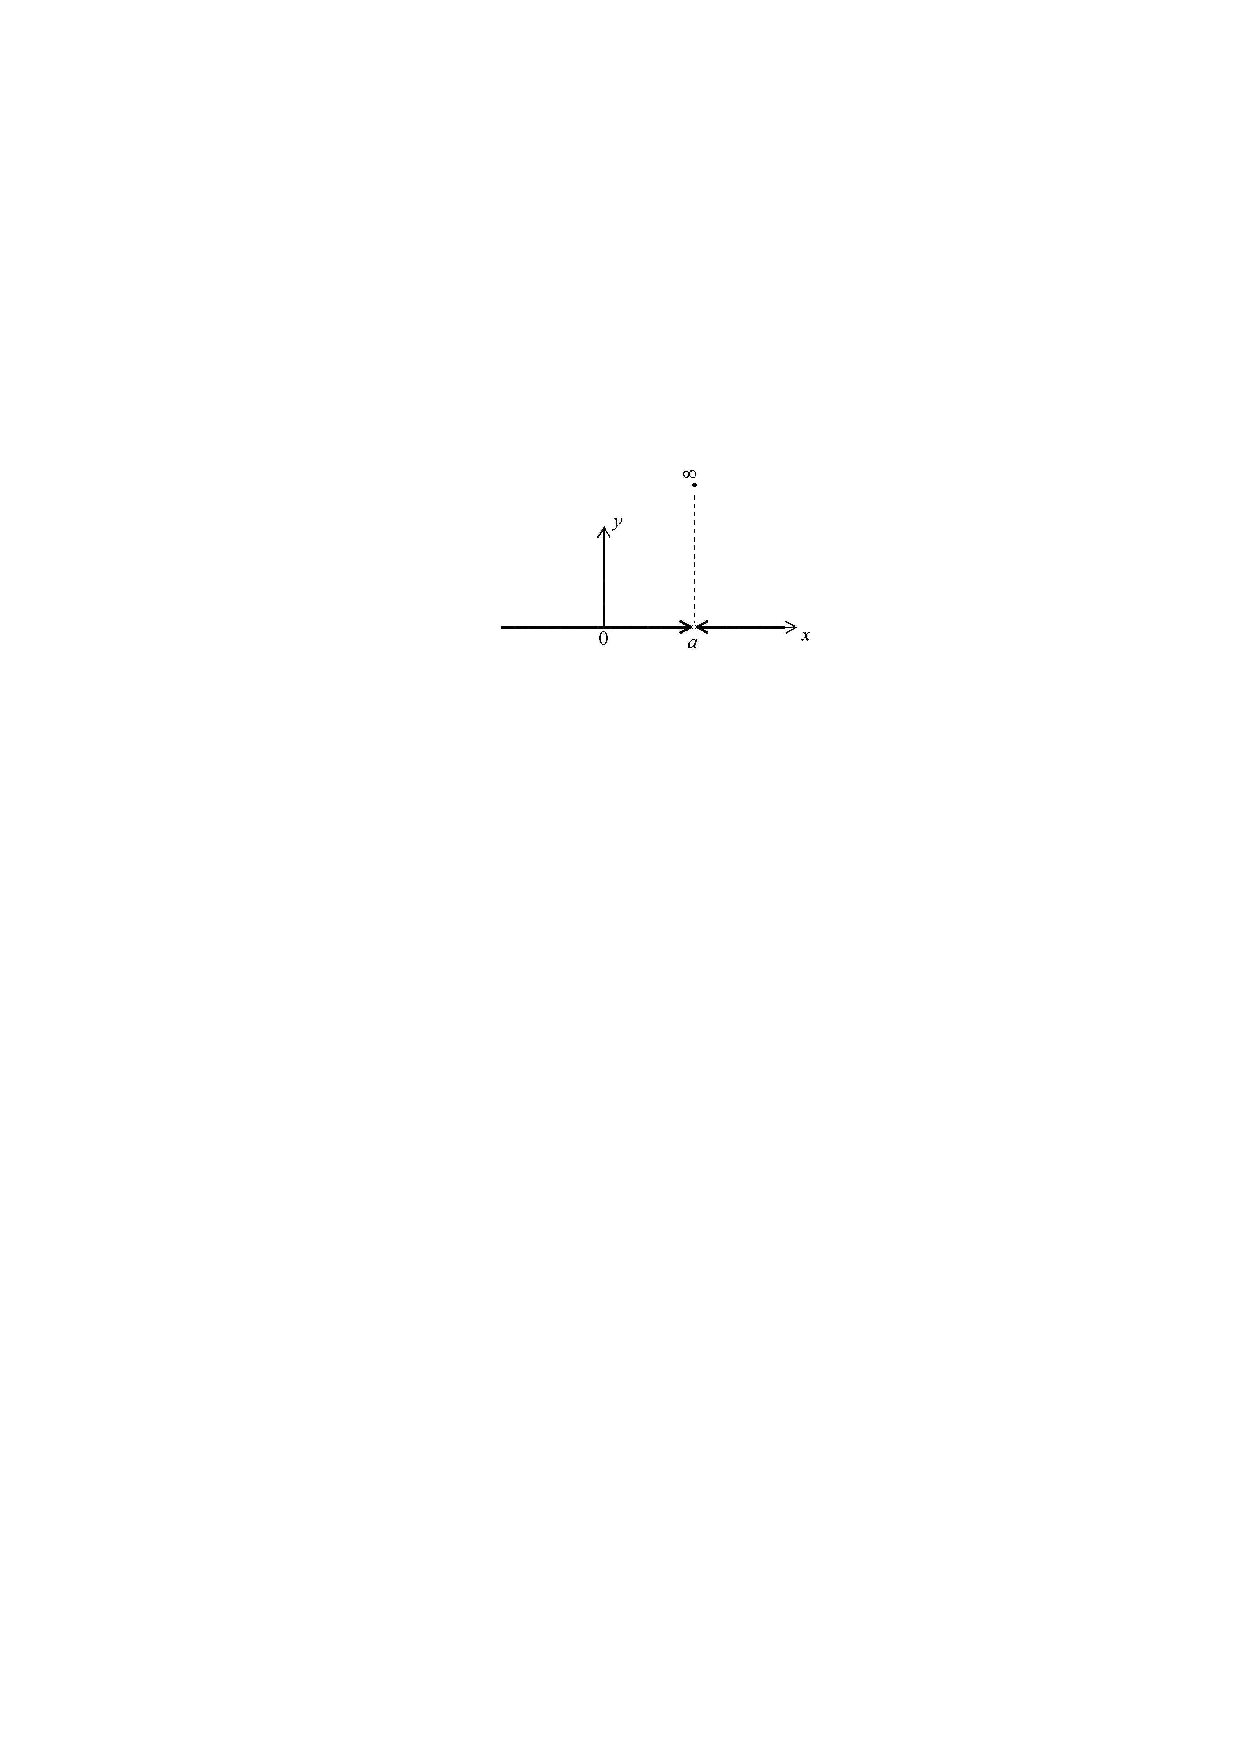
\includegraphics[]{pic/pic18}
	\caption{Функция $y=\delta(x-a)$}
	\label{fig18}
\end{figure}

\begin{prop}\-
\label{prop:13.5}
\begin{enumerate}
	\item  Для любого $c \in \mathbb{R}$ и любого $\varepsilon > 0$, имеет место формула
\begin{equation*}
	\int\limits_{c-\varepsilon}^{c+\varepsilon}\delta(x-c)dx=1
\end{equation*}
	\item Имеет место формула \begin{equation*}
		u(x)=\int\limits_{-\infty}^x\delta(t)dt
	\end{equation*}
	\item Имеет место формула \begin{equation*}
		u'(x)=\delta(x)
	\end{equation*}
	\item Для любой непрерывной функции $f(x)$ любого $a \in \mathbb{R}$ имеет место тождество
	\begin{equation*}
		f(x)\delta(x-a)=f(a)\delta(x-a).
	\end{equation*}
	\item Для любой непрерывной функции $f(x)$ любого $a \in \mathbb{R}$ имеет место тождество
	\begin{equation*}
		\int\limits_{-\infty}^{\infty}f(x)\delta(x-a)dt=f(a).
	\end{equation*}
	\item Для любой непрерывной функции $f(x)$ любого $a \in \mathbb{R}$ имеет место тождество
	\begin{equation*}
		\int\limits_{-\infty}^xf(t)\delta(t-a)dt=f(a)u(x-a),
	\end{equation*}
	в частности
	\begin{equation*}
		\int\limits_{-\infty}^x\delta(t-a)dt=u(x-a)
	\end{equation*}
	\item Если функция $f(x)$ непрерывна и все её нули (корни) $x_1, x_2,\dots , x_k, \dots$ простые (т.е. имеют кратность 1), то
	\begin{equation*}
		\delta(f(x))=\sum\limits_k\frac{\delta(x-x_k)}{|f'(x_k)|}.
	\end{equation*}
	\item Дельта-функция получается при вычислении преобразования Фурье
	от константы:
	\begin{equation*}
		\int\limits_{-\infty}^{\infty}e^{ixt}dt=2\pi \delta(x)
	\end{equation*}
\end{enumerate}
\end{prop}

\begin{example}\-
\label{ex:13.6}
\begin{enumerate}[leftmargin=1.1em]
	\item См.пример \ref{ex:13.2}.3. 

	Дано
	\begin{equation*}
		F_{\xi}(x)=\frac{x-a}{b-a}[u(x-a)-u(x-b)]+u(x-b).
	\end{equation*}

	Найти $f_{\xi}(x)$.

	\textit{Решение.}
	\begin{equation*}
	\begin{split}
		&f_{\xi}(x)=F'_{\xi}(x)=\\=
		&\left(\frac{x-a}{b-a}\right)'[u(x-a)-u(x-b)]+
		\frac{x-a}{b-a}\left[u(x-a)-u(x-b)\right]+\delta(x-b)=\\=
		%
		&\frac{1}{b-a}[u(x-a)-u(x-b)]+\frac{x-a}{b-a}[\delta(x-a)-\delta(x-b)]+
		\delta(x-b)=\\=
		%
		&\frac{1}{b-a}[u(x-a)-u(x-b)]+\frac{x-a}{b-a}\delta(x-a)
		-\frac{x-a}{b-a}\delta(x-b)+\delta(x-b)=\\=
		%
		&\frac{1}{b-a}[u(x-a)-u(x-b)]+\frac{a-a}{b-a}\delta(x-a)-\frac{b-a}{b-a}\delta(x-b)+\delta(x-b)=\\=
		&\frac{1}{b-a}[u(x-a)-u(x-b)].
	\end{split}
	\end{equation*}
	\item Найти плотность вероятности по данной функции распределения
	(см. рис. \ref{fig19})
	
	Дано.
	\begin{equation*}
		F_{\xi}(x)
		\left\{\begin{aligned}
			&0, &x<0 \\
			&\frac{1}{24}(5x+8), &0\leqslant x<2 \\
			&1, &x\geqslant 2
		\end{aligned}\right\}
		=\frac{1}{24}(5x+8)[u(x)-x(x-2)]+u(x-2).
	\end{equation*}

	\textit{Решение.}
	\begin{gather*}
		f_{\xi}(x)=F'_{\xi}(x)=\\=
		\frac{5}{24}[u(x)-u(x-2)]+\frac{1}{24}(5x+8)[\delta(x)-\delta(x-2)]+\delta(x-2)=\\=
		\frac{5}{24}[u(x)-u(x-2)]+\frac{1}{3}\delta(x)-\frac{3}{4}\delta(x-2)=\\=
		\frac{1}{3}\delta(x)+\frac{5}{24}[u(x)-u(x-2)]+\frac{1}{4}\delta(x-2).
	\end{gather*}
	См. рис. \ref{fig20}
\end{enumerate}
\end{example}

\begin{figure}[H]
	\centering
	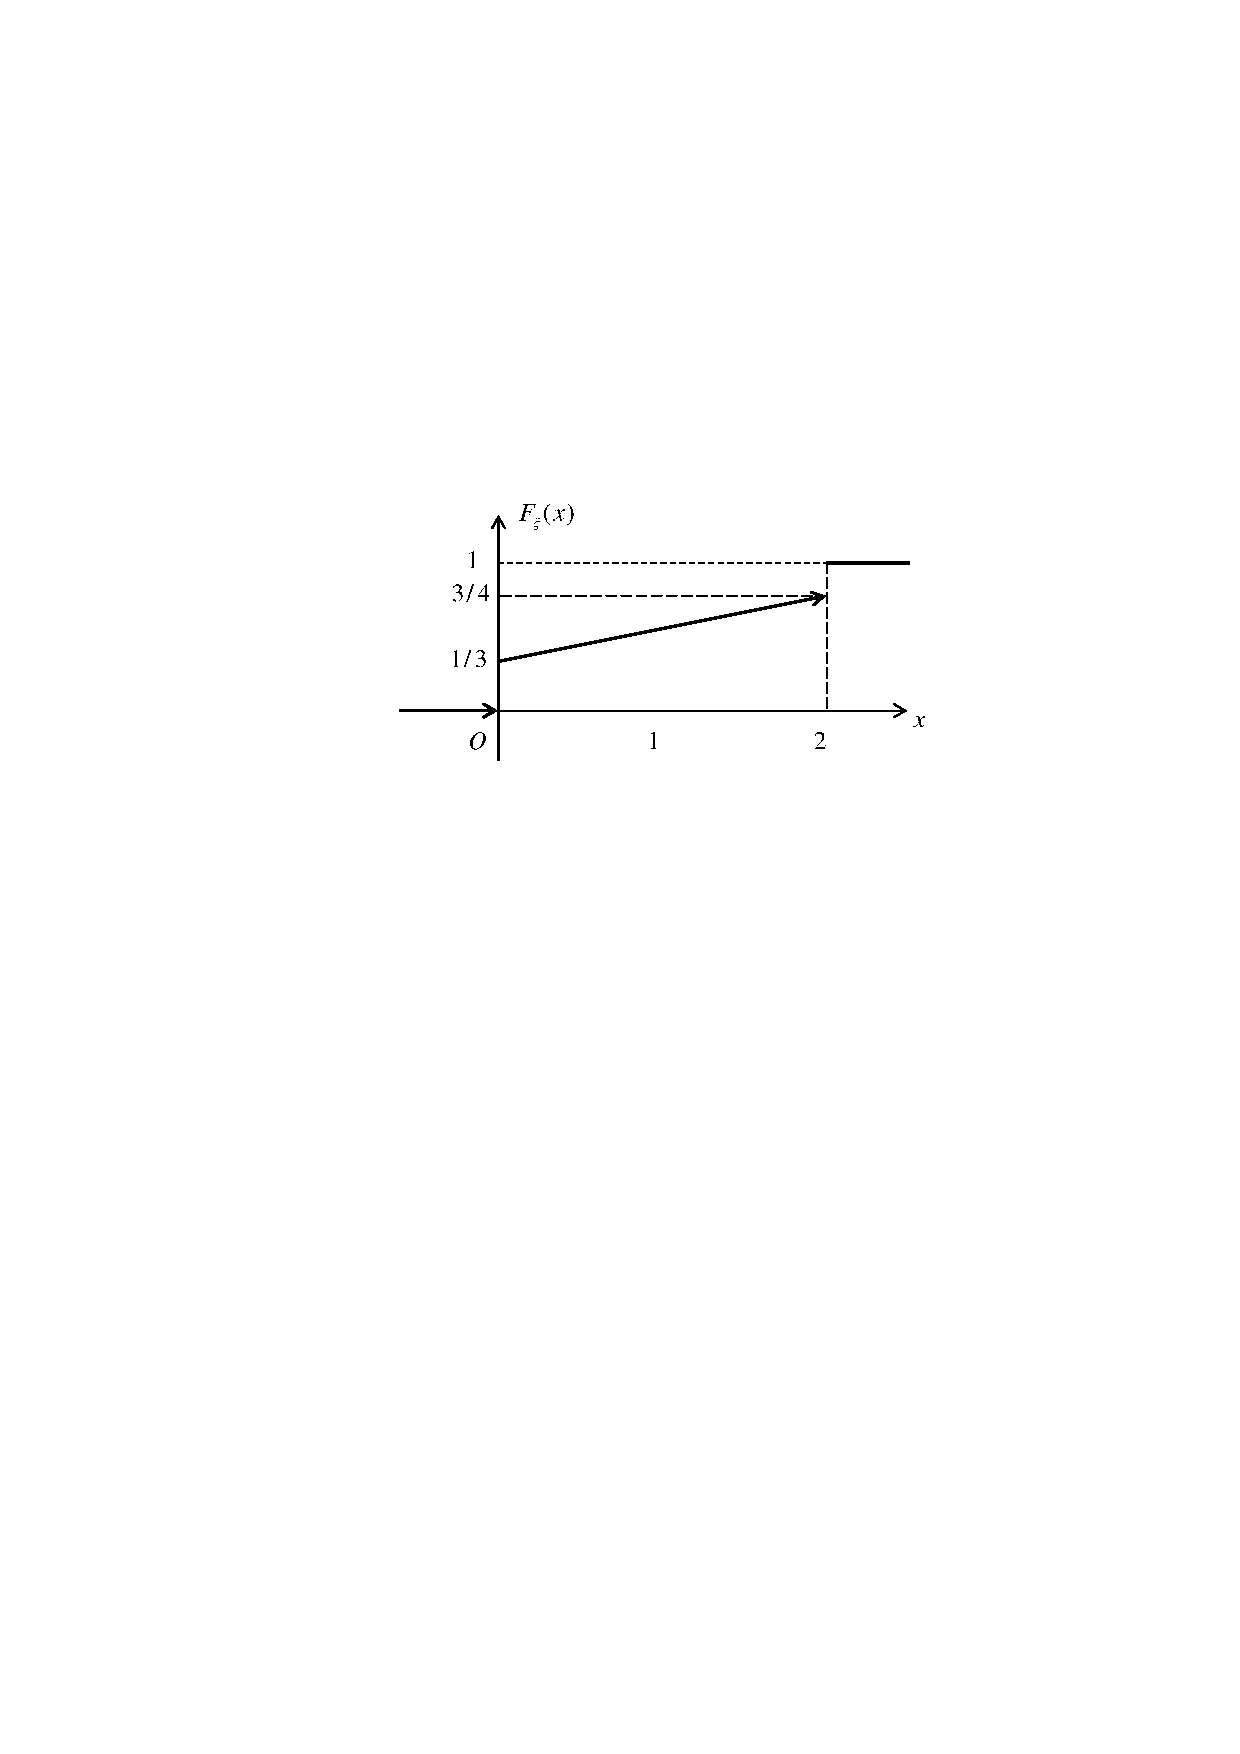
\includegraphics[]{pic/pic19}
	\caption{Функция распределения с двумя скачками}
	\label{fig19}
\end{figure}
\begin{figure}[H]
	\centering
	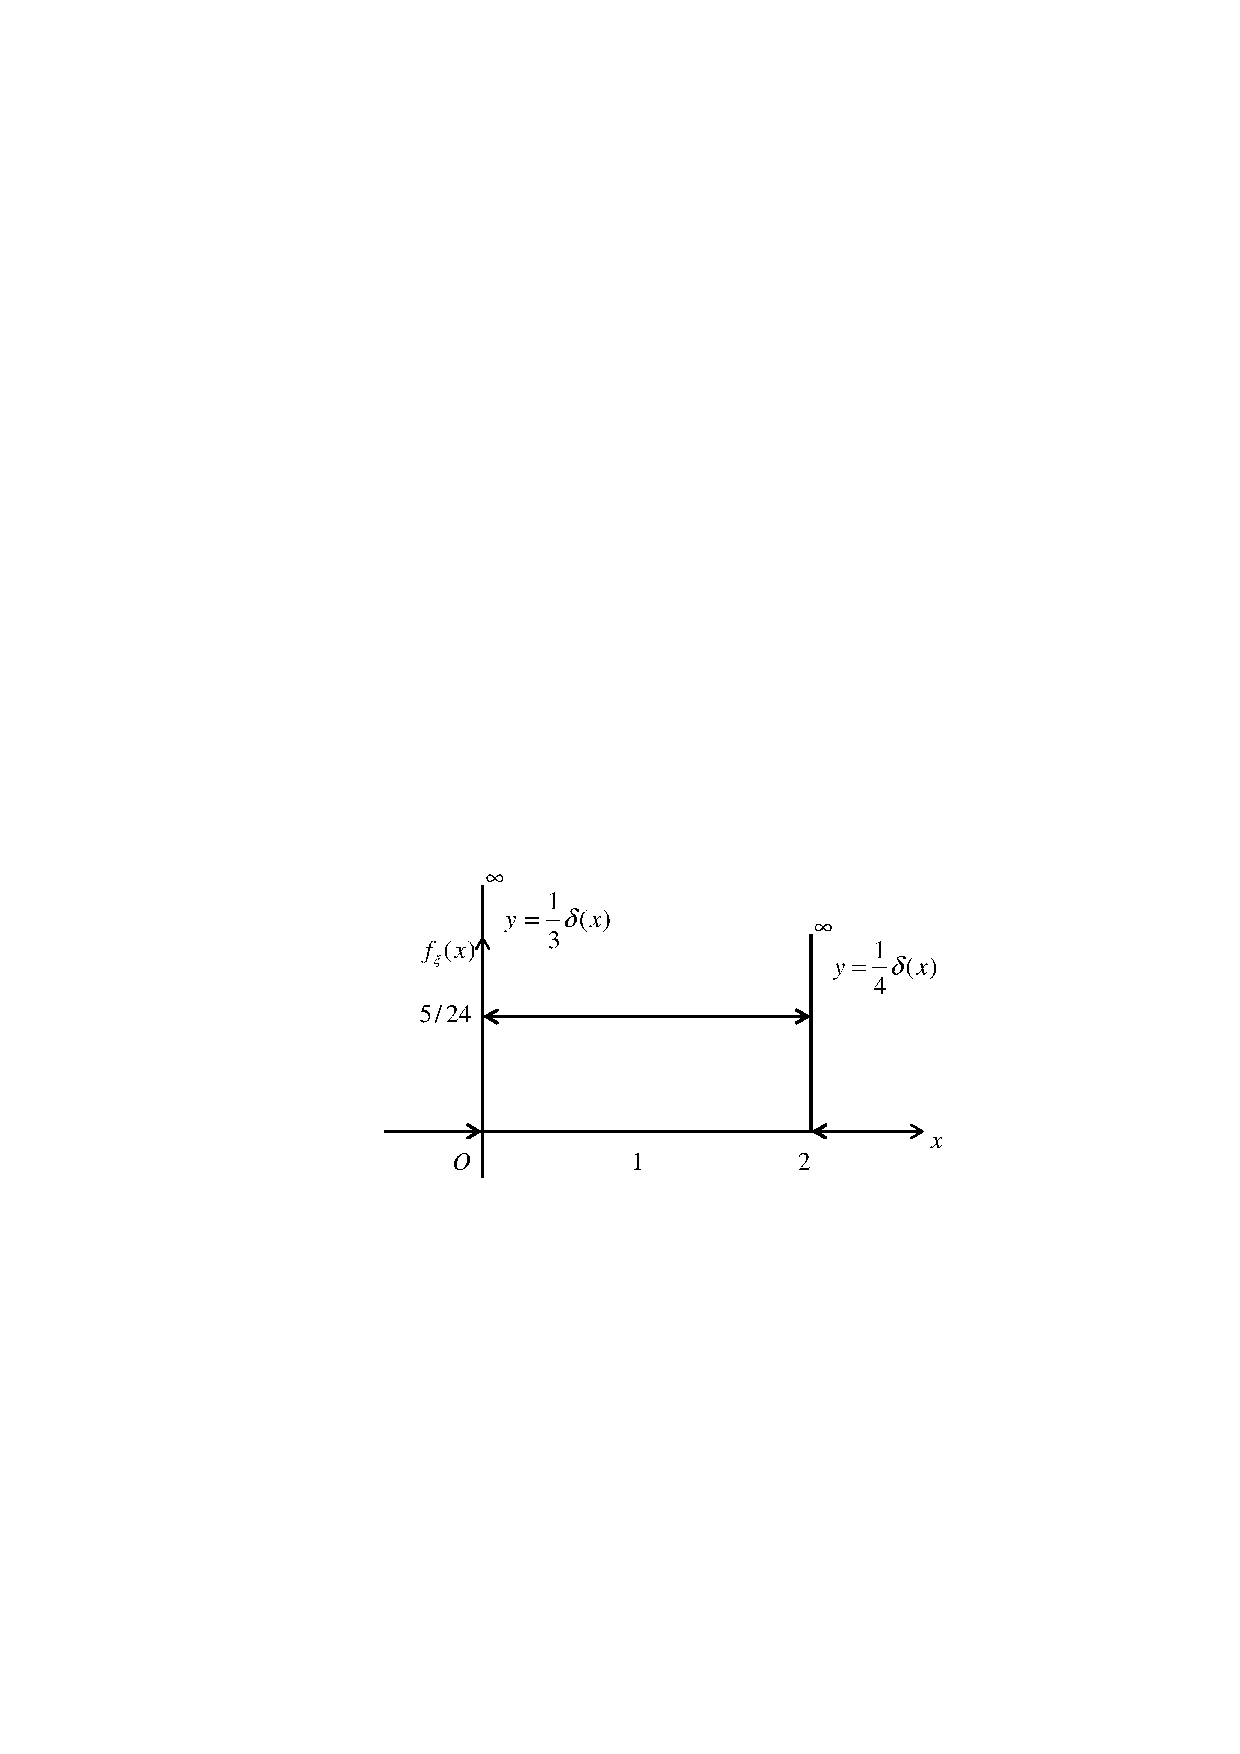
\includegraphics[]{pic/pic20}
	\caption{Площадь под плотностью равна 
				$\frac{1}{3}+\frac{5}{24}\cdot 2+\frac{1}{4}= 1$.}
	\label{fig20}
\end{figure}

\begin{definition}
\label{def:13.6}
	Функции Хевисайда и Дирака и их композиции относятся к классу так называемых обобщённых функций.
\end{definition} %кирилл

\section{Функции одной случайной величины}
%!TEX root = ../var.tex
\begin{zam}
Пусть $\xi : \Omega \to \mathbb{R}$ -- абсолютно непрерывная случайная величина, имеющая плотность $f_\xi (x)$. Построим с помощью функции $g : \mathbb{R} \to \mathbb{R}$ новую случайную величину по формуле $\eta = g(\xi)$. 

Требуется найти функцию распределения и плотность случайной величины $\eta$. Мы решим эту задачу сначала в предположении, что функция $y = g(x)$ дифференцируема и монотонна, т.е. когда во всех точках $x \in \mathbb{R}$ выполнено либо $g′(x) > 0$, либо $g′(x) < 0$.	
\end{zam}
\begin{theorem}
	\label{th:14.2}
Если $\xi$ -- абсолютно непрерывная случайная величина, имеющая функцию распределения $F_\xi (x)$ и плотность $f_\xi (x)$, и если $g :\mathbb{R} \to \mathbb{R}$ -- дифференцируемая и монотонная функция, то случайная величина $\eta = g(\xi)$ имеет плотность вероятности
\begin{equation*}
	f_\eta(y)=f_\xi\left(g^{-1}(y)\right)\left|\diff{[g^{-1}(y)]}{y}\right|
\end{equation*}
\end{theorem}
\begin{proof}
Заметим, что если $g :\mathbb{R} \to \mathbb{R}$  -- монотонная функция, то существует её функция$ g^{-1} :\mathbb{R} \to R$, и выполнено тождество
\begin{equation*}
	g(g^{-1}(y))\equiv y 	
\end{equation*} 
Дифференцируя его, получим тождество
\begin{equation*}
	g'(g^{-1}(y)) \cdot (g^{-1} (y))' \equiv 1,
\end{equation*}
которое означает, что производные $g′$ и $(g^{-1})'$ --
одного знака, т.е. функции $g$ и $g^{-1}$ либо обе возрастающие, либо обе убывающие.


1) Пусть сначала $g$ -- возрастающая функция, т.е. $g' > 0$ и $g^{-1} > 0$. Это означает, что неравенство $g(\xi) \leq y$ можно записать в виде $ \xi \leq g^{-1}(y)$.

\begin{gather*}
	F_{\eta}(y) = F_{g(\xi)}(y) = P(g(\xi) \leq y) = P(\xi \leq g^{-1} (y)) = F_\xi (g^{-1} (y)) =\\=
	\int\limits^{g^{-1}(y)}_{-\infty} f_\xi(t) dt=
	%
	\left[
	\begin{aligned}
		t = g^{-1} (\tau ),\qquad & dt = (g^{-1}(\tau ))' d\tau\\
		t = -\infty \mapsto \tau = -\infty,\quad & t = g^{-1}(y) \mapsto \tau = y
	\end{aligned}\right]=\\=
	\int\limits_{-\infty}^y (g^{-1}(\tau))' f_\xi(g^{-1}(\tau)) d\tau.
\end{gather*}



2) Пусть теперь $g$ -- убывающая функция, т.е. $g' < 0 $и $g^{-1} < 0$, тогда
неравенство $g(\xi) \leq y$ можно записать в виде $\xi \geq g^{-1} (y)$.

\begin{gather*}
	F_{\eta}(y) = F_{g(\xi)}(y) = P(g(\xi) \leq y) = P(\xi \geq g^{-1} (y)) =\\=
	\int\limits_{g^{-1}(y)}^{\infty} f_\xi(t) dt=
	%
	\left[
	\begin{aligned}
		t = g^{-1} (\tau ),\qquad & dt = (g^{-1}(\tau ))' d\tau\\
		t = -\infty \mapsto \tau = -\infty,\quad & t = g^{-1}(y) \mapsto \tau = y
	\end{aligned}\right]=\\=\int\limits^{-\infty}_y (g^{-1}(\tau))' f_\xi(g^{-1}(\tau)) d\tau=
	\int\limits_{-\infty}^y \left|(g^{-1}(\tau))'\right| f_\xi(g^{-1}(\tau)) d\tau.
\end{gather*}

Объединяя оба случая в один, получим требуемую формулу.
\end{proof}

\begin{definition}
\label{def:14.3}
Пусть $A$ – подмножество на прямой $\mathbb{R}$, т.е. $A \subset
\mathbb{R}$. Функция $\mathbf{1}_A :\mathbb{R} \to \{0, 1\}$, определённая по формуле
\begin{equation*}
	\mathbf{1}_A (x)=\left\{
	\begin{aligned}
		1, \text{ если } x\in A\\
		0, \text{ если } x\notin A
	\end{aligned}
	\right.
\end{equation*}
называется выделяющей функцией множества $A$ или индикатором $A$.
Если $A = [0, \infty)$, то обозначение $\mathbf{1}_A(x)$ сокращают до $\mathbf{1}(x)$. Заметим, что $\mathbf{1}(x) = u(x)$, т.е. совпадает с функцией Хевисайда.	
\end{definition}

\begin{zam}
Пусть теперь $g : \mathbb{R} \to \mathbb{R}$, $y = g(x)$ -- дифференцируемая, кусочно монотонная функция, имеющая интервалы монотонности:
\begin{equation*}
	\mathcal{D}=\{D1=(-\infty, a_1], D_2 = (a_1 , a_2 ], \ldots , D_n = (a_{n-1} , \infty)\} 
\end{equation*}

Ясно, что все ограничения $g|_{D_i} : D_i \to \mathbb{R}$, определённые по формулам $g|_{D_i}(x)=g(x)$ являются взаимно однозначными функциями и поэтому имеют обратные $\left(g|_{D_i}\right)^{-1}(y)={g|_{D_i}}^{-1}(y)$ с областями определения $g(D_i)$ соответственно.
\end{zam}

\begin{theorem}[Без доказательства]
	\label{th:14.5}
Если $\xi $ -- абсолютно непрерывная случайная величина, имеющая функцию распределения $F_\xi (x)$ и плотность $f\xi (x)$, и если $g : \mathbb{R} \to \mathbb{R}$ -- кусочно дифференцируемая и кусочно монотонная функция на интервалах $\mathcal{D}$, то случайная величина $\eta = g(\xi)$ имеет плотность вероятности
\begin{equation*}
	f_\eta(y)=\sum\limits_{i=1}^n f_\xi\left(
		{g|_{D_i}}^{-1}(y)
	\right)\cdot
	\left|
		\diff{\left[ {g|_{D_i}}^{-1}(y) \right]}{y}\cdot\mathbf{1}_{g(D_i)}(y)
	\right|
\end{equation*}

\end{theorem}
%федя

\section{Случайные векторы и их распределения} 
%!TEX root = ../var.tex

Пусть $(\Omega,\mathfrak{A},\P)$-- произвольное вероятностное пространство.

\begin{definition}
\label{def:15.1}
	Вектор $(\xi_1, \dots, \xi_n)$ называется случайным вектором, если $\xi_1, \dots, \xi_n$ являются случайными величинами, заданными на одном
и том же вероятностном пространстве $\Omega$.
\end{definition}

\begin{definition}
\label{def:15.2}
	Функцией совместного распределения случайных
величин $(\xi_1, \dots, \xi_n)$ (или случайного вектора $(\xi_1, \dots, \xi_n)$) называется функция $F_{\xi_1, \dots, \xi_n} : \mathbb{R}^n \rightarrow [0, 1]$, определённая по формуле
\begin{equation*}
	F_{\xi_1, \dots, \xi_n}(x_1,\dots,x_n)=\P(\xi_1\leqslant x_1,\dots,\xi_n\leqslant x_n).
\end{equation*}

Ясно, что $0 \leqslant F_{\xi_1, \dots, \xi_n}(x_1,\dots,x_n) \leqslant 1$

\end{definition}

\begin{definition}
\label{def:15.3}
	Говорят, что случайные величины $(\xi_1, \dots, \xi_n)$ имеют абсолютно непрерывное совместное распределение, если существует
такая неотрицательная функция $f_{\xi_1, \dots, \xi_n}(x_1,\dots,x_n)$, что для любой точки
$(x_1,\dots,x_n)\in\mathbb{R}^n$ функция распределения $F_{\xi_1, \dots, \xi_n}(x_1,\dots,x_n)$ представима в
виде
\begin{equation*}
	F_{\xi_1, \dots, \xi_n}(x_1,\dots,x_n)=\int\limits_{-\infty}^{x_1}\ldots
	\int\limits_{-\infty}^{x_n}f_{\xi_1, \dots, \xi_n}(t_1,\dots,t_n)dt_1\ldots dt_n.
\end{equation*}
При этом функция $f_{\xi_1, \dots, \xi_n}(x_1,\dots,x_n)$ называется плотностью вероятности совместного распределения случайных величин ${\xi_1, \dots, \xi_n}$.
\end{definition}

\begin{lemma}
\label{lemma:15.4}
Справедлива формула
	\begin{equation*}
		f_{\xi_1, \dots, \xi_n}(x_1,\dots,x_n)=\frac
		{\partial^nF_{\xi_1, \dots, \xi_n}(x_1,\dots,x_n)}
		{\partial x_1\ldots \partial x_n}.
	\end{equation*}
\end{lemma}

\begin{proof}
	Формула получается в результате последовательного дифференцирования формулы определения \ref{def:15.3} по верхним пределам.
\end{proof}

\begin{definition}
\label{def:15.5}
	Случайные величины $\xi_1, \dots, \xi_n$ называются независимыми, если для любого набора множеств $A_1,\dots ,A_n \subset \mathbb{R}$, такого что\newline
 	$\xi_1^{-1}(A_1), \dots, \xi_n^{-1}(A_n)\in\mathfrak{A}$ иммет место равенство
 	\begin{equation*}
 		\P(\xi_1\in A_1,\dots,\xi_n\in A_n)=\P(\xi_1 \in A_1)\cdot\ldots\cdot\P(\xi_m\in A_n).
 	\end{equation*}
\end{definition}

 \begin{lemma}\-
\label{lemma:15.6}

 \begin{enumerate}
 	\item Случайные величины независимы, если для любых $$x_1,\dots, x_n \in \mathbb{R}$$ имеет место равенство
 	\begin{equation*}
 		F_{\xi_1, \dots, \xi_n}(x_1,\dots,x_n)=F_{\xi_1}(x_1)\cdot\ldots\cdot F_{\xi_n}(x_n).
 	\end{equation*}
 	\item Случайные величины независимы, если для любых $x_1,\ldots,x_n\in\mathbb{R}$ имеет место равенство
 	\begin{equation*}
		f_{\xi_1, \dots, \xi_n}(x_1,\dots,x_n)=f_{\xi_1}(x_1)\cdot\ldots\cdot f_{\xi_n}(x_n). 		
 	\end{equation*}
 \end{enumerate}
\end{lemma}

\begin{proof}\-

	1)
	\begin{gather*}
	F_{\xi_1, \dots, \xi_n}(x_1,\dots,x_n)=\P(\xi_1\leqslant x_1,\ldots,\xi_n
	\leqslant x_n)=\\=
	\P(\xi_1\leqslant x_1)\cdot\ldots\cdot\P(\xi_n\leqslant x_n)=F_{\xi_1}(x_1)\cdot\ldots\cdot F_{\xi_n}(x_n).
	\end{gather*}	

	2)
	\begin{gather*}
	f_{\xi_1,\ldots,\xi_n}(x_1,\ldots,x_n)=
		\frac
		{\partial^nF_{\xi_1, \dots, \xi_n}(x_1,\dots,x_n)}
		{\partial x_1\ldots \partial x_n}=
		\frac
		{\partial^n\left[F_{\xi_1}(x_1)\cdot\ldots\cdot F_{\xi_n}(x_n)\right]}
		{\partial x_1\ldots \partial x_n}=\\=
		\frac{\partial F_{\xi_1}(x_1)}{\partial x_1}\cdot\ldots\cdot
		\frac{\partial F_{\xi_n}(x_n)}{\partial x_n}=f_{\xi_1}(x_1)\cdot\ldots\cdot f_{\xi_n}(x_n).
	\end{gather*}
\end{proof}

В следующей теореме без потери общности и для простоты формулировки мы ограничимся двухмерным случаем, $n = 2$.

\begin{theorem}[Свойства функции распределения, без доказательства]
\label{th:15.7}
.
\begin{enumerate}
	\item Функция $F_{\xi_1,\xi_2}(x_1,x_2)$ является неубывающей по каждому аргументу $x_1$ и $x_2$.

	\item Существуют пределы 
	\begin{gather*}
	F_{\xi_1,\xi_2}(-\infty,x_2)=\lim\limits_{x_1\to-\infty}
	F_{\xi_1,\xi_2}(x_1,x_2)=0 \\
	F_{\xi_1,\xi_2}(x_1,-\infty)=\lim\limits_{x_2\to-\infty}
	F_{\xi_1,\xi_2}(x_1,x_2)=0
	\end{gather*}

	\item Существуют пределы 
	\begin{gather*}
	F_{\xi_1,\xi_2}(\infty,x_2)=\lim\limits_{x_1\to\infty}
	F_{\xi_1,\xi_2}(x_1,x_2)=F_{\xi_2}(x_2) \\
	F_{\xi_1,\xi_2}(x_1,\infty)=\lim\limits_{x_2\to\infty}
	F_{\xi_1,\xi_2}(x_1,x_2)=F_{\xi_1}(x_1)
	\end{gather*}

	\item Справедливо
	\begin{gather*}
	f_{\xi_1}(x_1)=\int\limits_{-\infty}^{\infty}f_{\xi_1,\xi_2}(x_1,x_2)dx_2, \\
	f_{\xi_2}(x_2)=\int\limits_{-\infty}^{\infty}f_{\xi_1,\xi_2}(x_1,x_2)dx_1,
	\end{gather*}

	\item $F_{\xi,\eta}(x, y)$ непрерывна справа по каждой координате x и y.



\end{enumerate}

\end{theorem}

\begin{example}\-
\label{ex:15.8}
	\begin{enumerate}
		\item Пусть $A \subset \mathbb{R}_n$ — множество, имеющее конечный
			объём $\mu(A)$, в пространстве с координатами $x = (x_1,\dots, x_n)$. Тогда функция
			\begin{equation*}
				f_{\xi_1,\dots,\xi_n}(x_1,\dots,x+n)=
				\begin{cases}
					\frac{1}{\mu(A)}, &\text{ если } x\in A\\
					0, &\text{ если } x\notin A\\
				\end{cases}
			\end{equation*}
			определяет плотность случайного вектора $\{\xi_1,\dots,\xi_n\}$ с равномерным распределением в $A$.
	\end{enumerate}
		\item Функция $f_{\xi,\eta}(x,y)=$
		\begin{equation*}
			=\frac{1}{2\pi\sigma_1\sigma_2\sqrt{1-r^2}}\exp
			\left\{
				-\frac{1}{2(1-r^2)}
			\left[
				\frac{(x-a)^2}{\sigma_1^2}-\frac{2r(x-a)(y-b)}{\sigma_1\sigma_2}+\frac{(y-b)^2}{\sigma_2^2} 
			\right] 
			\right\},
		\end{equation*}
		где $r$ — коэффициент корреляции (см. \S\ref{par:18}), определяет двухмерную нормальную плотность вероятности случайного вектора $(\xi, \eta)$, показанную на рис. \ref{fig21}. Там же показан эллипс равных вероятностей
		\begin{equation*}
			\frac{(x-a)^2}{\sigma_1^2}-\frac{2r(x-a)(y-b)}{\sigma_1\sigma_2}+\frac{(y-b)^2}{\sigma_2^2}=const
		\end{equation*}
\begin{figure}[H]
	\centering
	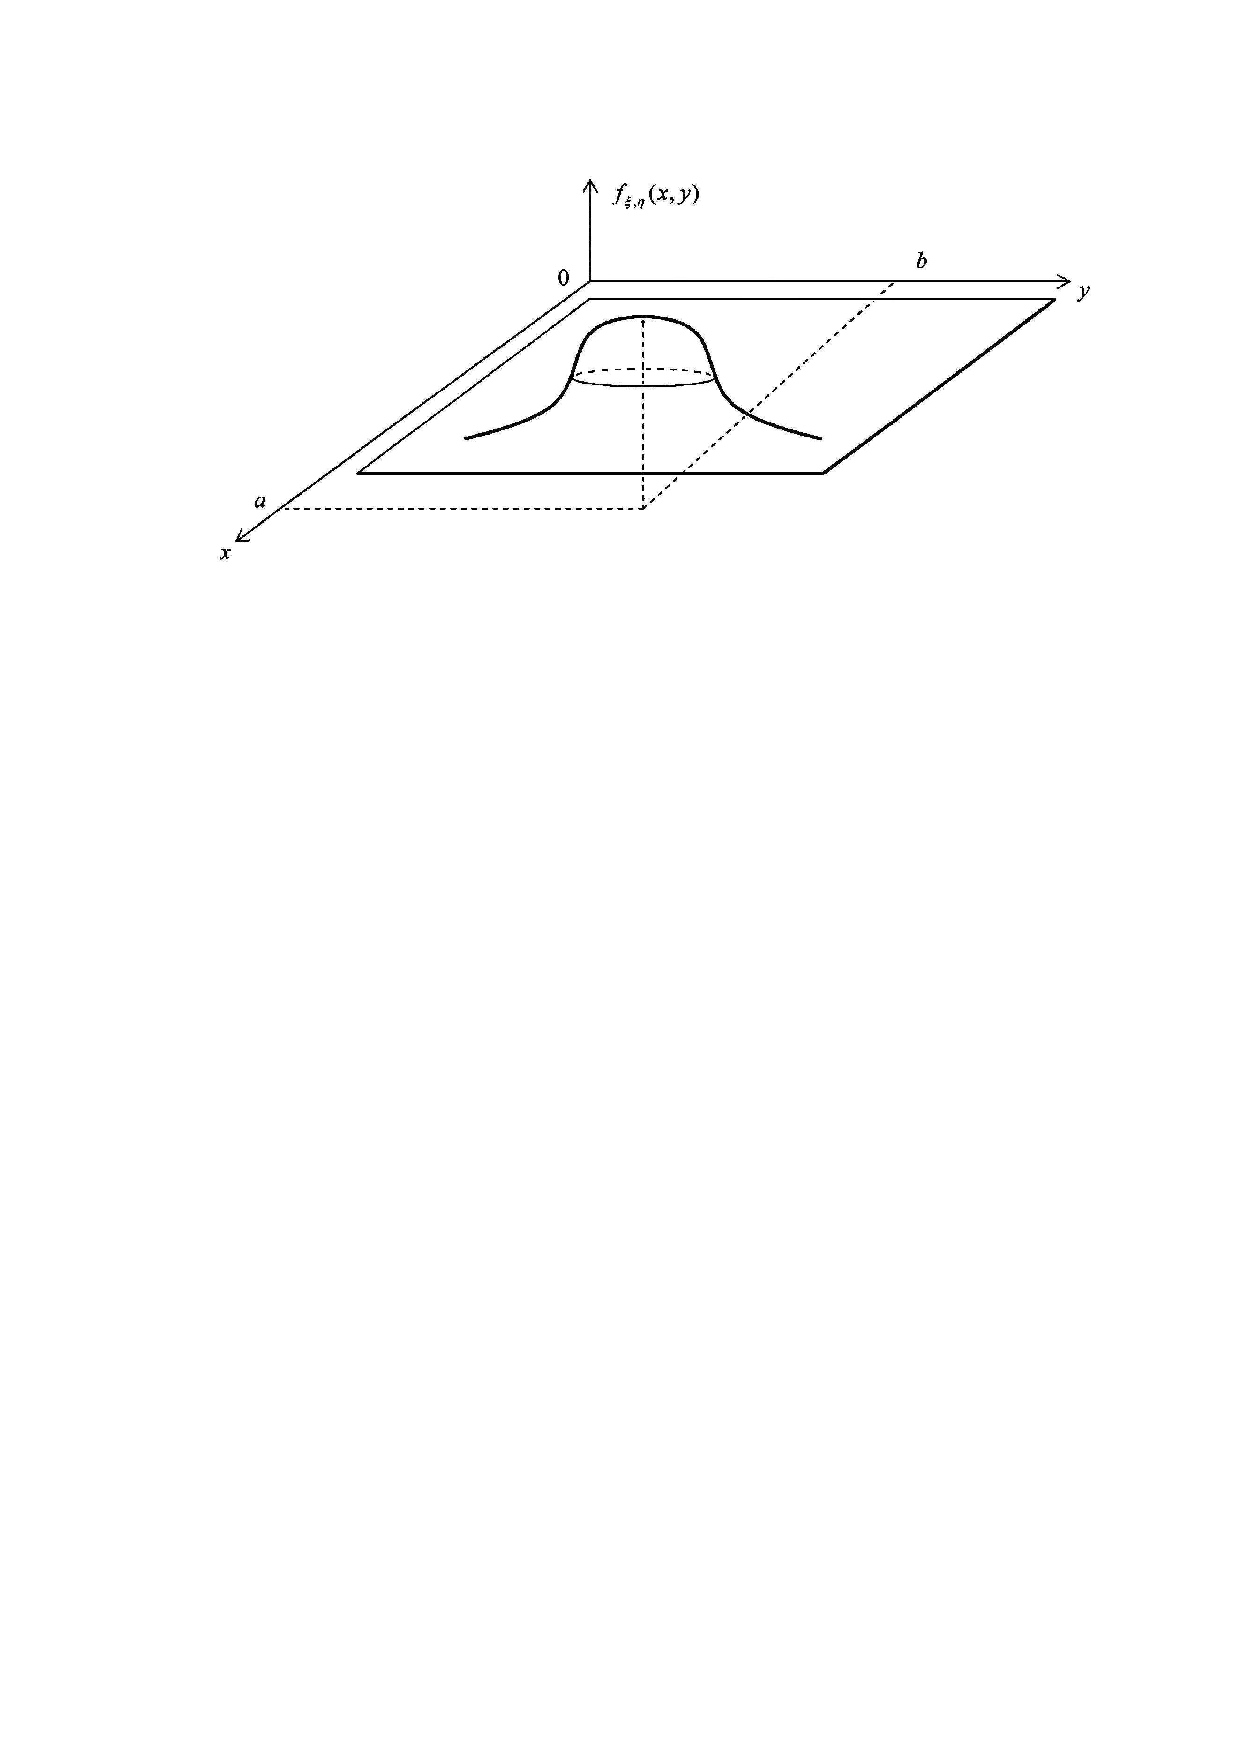
\includegraphics[]{pic/pic21}
	\caption{Плотность вероятности двухмерного нормального распределения.}
	\label{fig21}
\end{figure}
\end{example}
%кирилл

\section{Функции от двух случайных величин} 
%!TEX root = ../var.tex
\begin{zam}
Пусть $\xi_1 , \xi_2$ -- случайные величины с совместной плотностью вероятности $f_{\xi_1} ,\xi_2 (x_1 , x_2 )$. Построим с помощью функции $g : \mathbb{R}^2 \to \mathbb{R}$ случайную величину $\eta = g(\xi_1 , \xi_2 )$. Требуется найти функцию распределения $F_\eta (y)$ и плотность вероятности $f_\eta (y)$ случайной величины $\eta$.
\end{zam}

\begin{lemma}
Пусть $y \in \mathbb{R}$, и область $D_y \subseteq \mathbb{R}^2$ состоит из точек $(x_1 , x_2 )$, удовлетворяющих неравенству $g(x_1 , x_2 ) \leq y$, т.е. $D_y = \{(x_1 , x_2 ) \in \mathbb{R}^2 | g(x_1 , x_2 ) \leq y\}$. Тогда случайная величина $\eta = g(\xi_1 , \xi_2 )$ имеет функцию распределения
\begin{gather*}
	F_\eta (y) = \iint\limits_{D_y}f_{\xi_1} ,\xi_2 (x_1 , x_2 ) dx_1 dx_2
\end{gather*}
\end{lemma}

\begin{proof}
\begin{gather*}
	F_\eta (y) = \P ( g(x_1 , x_2 ) \leq y ) = \P( (x_1 , x_2 ) \in Dy )= \iint\limits_{D_y}f_{\xi_1} ,\xi_2 (x_1 , x_2 ) dx_1 dx_2
\end{gather*}

где последнее равенство следует их того, что вероятность попадания случайного вектора $(x_1 , x_2 )$ в область $D_y$ равна объёму цилиндра, ограниченного сверху графиком плотности вероятности, а снизу -- областью $D_y$.
\end{proof}

\begin{figure}[h!]
	\centering
	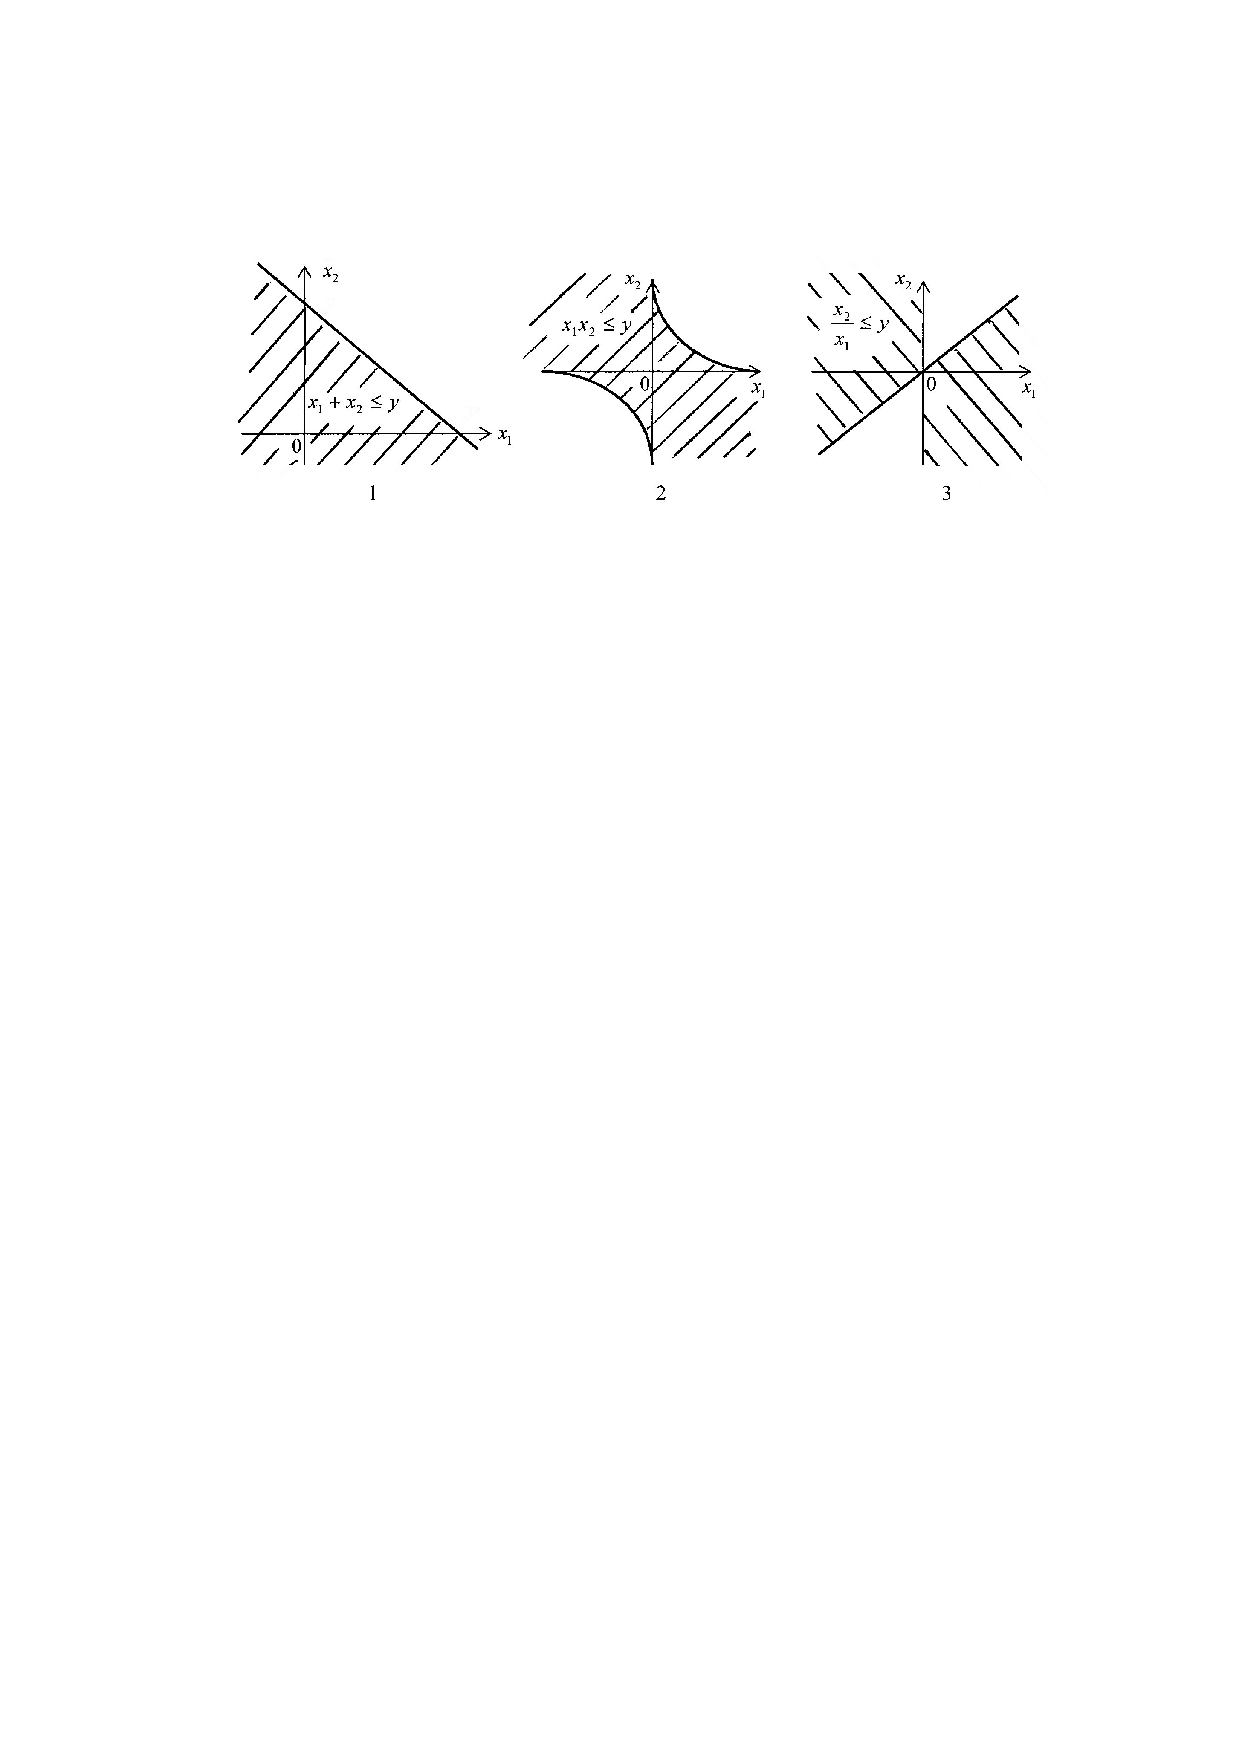
\includegraphics[]{pic/pic22}
	\caption{Случайные функции суммы, произведения и частного}
	\label{fig22}
\end{figure}

\begin{lemma}[Распределение суммы]
Пусть $\eta = \xi_1 + \xi_2$, тогда

\begin{gather*}
	F_\eta (y) = \P ( \eta \leq y ) = \P(x_1+x_2 \leq y )=
	\int\limits_{-\infty}^{\infty}\left(
		\int\limits_{-\infty}^{y-x_1 } f_{\xi_1,\xi_2} (x_1 , x_2 ) dx_2
	\right)dx_1
\end{gather*}
\end{lemma}
\begin{proof}
Воспользуемся леммой 16.2 для функции $g(x_1 , x_2 )=x_1 + x_2$. 

Заменим двойной интеграл по области $D_y = \{(x_1 , x_2 ) \in \mathbb{R}^2 | x_1 +
x_2 \leq y\}$ (см. рис. \ref{fig22}.1) на повторный, получим требуемый результат.	
\end{proof}

\begin{lemma}[Распределение произведения]
	
Пусть $\eta = \xi_1 \xi_2$ , тогда

\begin{gather*}
	F_\eta (y) = \P ( x_1x_2 \leq y ) =
	\int\limits_{-\infty}^{0}\left(
		\int\limits_{y/x_1}^{\infty} f_{\xi_1,\xi_2} (x_1, x_2 ) dx_2
	\right)dx_1+\\+
	\int\limits_{0}^{\infty}\left(
		\int\limits^{y/x_1}_{-\infty} f_{\xi_1,\xi_2} (x_1, x_2 ) dx_2
	\right)dx_1
\end{gather*}
\end{lemma}

\begin{proof}
	Воспользуемся леммой 16.2 для функции $g(x_1 , x_2 ) = x_1 x_2$.

Область $D_y = \{(x_1 , x_2 ) \in \mathbb{\mathbb{R}} x_1 x_2 \leq y\}$ показана на рис. \ref{fig22}.2. Переходя от двойного интеграла к повторному, получим требуемый результат.
\end{proof}

\begin{lemma}[Распределение частного]
Пусть $\eta = \frac{\xi_2}{\xi_1}$, тогда
\begin{gather*}
	F_\eta (y) = \P ( \frac{x_2}{x_1} \leq y ) =
	\int\limits_{-\infty}^{0}\left(
		\int\limits_{yx_1}^{\infty} f_{\xi_1,\xi_2} (x_1, x_2 ) dx_2
	\right)dx_1+\\+
	\int\limits_{0}^{\infty}\left(
		\int\limits^{yx_1}_{-\infty} f_{\xi_1,\xi_2} (x_1, x_2 ) dx_2
	\right)dx_1
\end{gather*}
\end{lemma}
\begin{proof}
Доказательство. Воспользуемся леммой 16.2 для функции $g(x_1 , x_2 ) = \frac{x_2}{x_1}$.

Область $D_y = \{(x_1 , x_2 ) \in \mathbb{R}^2  \frac{x_2}{x_1} \leq y\}$ показана на рис. \ref{fig22}.3 Переходя от двойного интеграла к повторному, получим требуемый результат.
\end{proof}

\begin{lemma}[О свёртке]
	Если случайные величины $\xi_1$ и $\xi_2$ независимы
и имеют плотности вероятности соответственно $f_{\xi_1} (x_1 )$ и $f_{\xi_2} (x_2 )$, то плотность вероятности суммы $\eta = \xi_1 + \xi_2$ равна свёртке плотностей $f_{\xi_1}$ и $f_{\xi_2}$:
\begin{gather*}
	f_\eta (t)=f_{\xi_1+\xi_2}(t)=\int\limits_{-\infty}^{\infty} f_{\xi_1} (u)f_{\xi_2} (t - u) du=
	\int\limits_{-\infty}^{\infty} f_{\xi_2}(u)f_{\xi_1} (t - u) du
\end{gather*}
\end{lemma}

\begin{proof}
Воспользуемся леммой 16.3
\begin{gather*}
	F_\eta (y) =
	\int\limits_{-\infty}^{\infty}\left(
		\int\limits_{-\infty}^{y-x_1 } f_{\xi_1,\xi_2} (x_1 , x_2 ) dx_2
	\right)dx_1=
	\int\limits_{-\infty}^{\infty}\left(
		\int\limits_{-\infty}^{y-x_1 } f_{\xi_1}(x_1)f_{\xi_2}(x_2) dx_2
	\right)dx_1
\end{gather*}

Сделаем в последнем интеграле замену переменной: $x_2 = t - x_1$ , $dx_2 = dt$.
При этом $x_2 \in (-\infty, x - x_1 )$ перейдёт в $t \in (-\infty, x)$. В последнем интеграле меняем порядок интегрирования и получаем:
\begin{gather*}
	\int\limits_{-\infty}^{\infty}\left(
		\int\limits_{-\infty}^{x} f_{\xi_1}(x_1)f_{\xi_2}(t-x_1) dt
	\right)dx_1=
	\int\limits_{-\infty}^{x}\overbrace{\left(
		\int\limits_{-\infty}^{\infty} f_{\xi_1}(x_1)f_{\xi_2}(t-x_1) dx_1
	\right)}^{f_{\xi_1+\xi_2}(t)}dt=
\end{gather*}

Итак, мы представили функцию распределения $F_\eta (x) = F_{\xi_1 +\xi_2} (x)$ в виде $\int\limits_{-\infty}^{x} f_{\xi_1 +\xi_2} (t) dt$, где

\begin{gather*}
	f_{\xi_1 +\xi_2} (t)=\int\limits_{-\infty}^{\infty} f_{\xi_1}(x_1)f_{\xi_2}(t-x_1) dx_1=\int\limits_{-\infty}^{\infty} f_{\xi_1}(u)f_{\xi_2}(t-u) du
\end{gather*}

Второе равенство теоремы получается из первого, если всюду в доказательстве поменять местами индексы 1 и 2.
\end{proof}

\begin{definition}
Если две независимые случайные величины имеют одно и то же распределение (возможно, с разными параметрами), и их сумма имеет то же самое распределение, то распределение называется устойчивым относительно суммирования.
\end{definition}

\begin{zam}
Следующие леммы могут быть доказаны непосредственно с помощью формулы свёртки, однако более короткие доказательства будут приведены в параграфе 25, используя характеристические функции.
\end{zam}

\begin{lemma}
	Пусть независимые случайные величины $\xi_n$ и $\xi_m$ имеют
биномиальное распределение (см. опред 12.8), с параметрами $n$ и $m$ и вероятностью "успеха" p, тогда случайная величина $\xi_n + \xi_m$ имеет биномиальное распределение $\xi_{n+m}$ . Другими словами, биномиальное распределение является устойчивым относительно суммирования.
\end{lemma}

\begin{lemma}
Пусть независимые случайные величины $\xi$ и $\eta$ имеют
нормальное распределение (см. опред 12.8), и имеют соответственно математические ожидания $a_1$ и $a_2$ и дисперсии $\sigma_1^2$ и $\sigma_2^2$, тогда случайная величина $\xi + \eta$ имеет нормальное распределение с математическим ожиданием $a_1 + a_2$ и дисперсией $\sigma_1^2+\sigma_2^2$. Другими словами, нормальное распределение является устойчивым относительно суммирования.	
\end{lemma}

\textbf{Пример}. Товарняк состоит из 100 вагонов. Масса (измеряемая в тоннах т) произвольного вагона -- случайная величина, распределенная по нормальному закону с средним значением 65 тонн и среднеквадратичным отклонением 9 тонн. Локомотив может везти состав массой не более 6600 тонн, в противном случае необходимо прицеплять второй локомотив. Найти вероятность того, что второй локомотив не потребуется.

\textit{Решение}. По лемме 16.10 имеем $a = a_1 + \ldots + a_100 = 65 \ldots 100 = 6500$, $\sigma = \sigma_1^2 +\ldots+\sigma_100^2=81\cdot100 = 8100$.

Вероятность того, что второй локомотив не потребуется, составляет $\P(\xi \leq 6600) = F_\xi (6600)=\frac{1}{2}+\Phi(\frac{x-a}{\sigma})=\frac{1}{2}+\Phi(\frac{6600-6500}{90})=\frac{1}{2}+\Phi(\frac{10}{9})\approx\frac{1}{2}+\Phi(1.11)\approx0.87$, где $\Phi(z) = \frac{1}{\sqrt{2\pi}}\int\limits_0^z e^{-t^2/2}dt$ -- табличный интеграл вероятности нормального распределения. %федя

\section{Математическое ожидание} 
%!TEX root = ../var.tex
\begin{definition}
	\begin{enumerate}
		\item Начальным моментом n-го порядка дискретной
		случайной величины $\xi$ называется число
		\begin{equation*}
			\M \xi^n=\sum\limits_kx_k^np_k.
		\end{equation*}
		\item Начальным моментом n-го порядка абсолютно непрерывной
		случайной величины $\xi$ называется число
		\begin{equation*}
			\M\xi^n=\int\limits_{-\infty}^{\infty}x^nf_{\xi}(x)dx.
		\end{equation*}
	\end{enumerate}
\end{definition}

\begin{definition}
\begin{enumerate}
	\item Математическим ожиданием или средним значением дискретной случайной величины $\xi$ называется начальный момент 1-го порядка
	\begin{equation*}
		\M \xi=\sum\limits_k x_kp_k
	\end{equation*}
	\item Математическим ожиданием или средним значением абсолютно непрерывной случайной величины $\xi$ называется начальный момент 1-го порядка
	\begin{equation*}
		\M\xi=\int\limits_{-\infty}^{\infty} xf_{\xi}(x) dx.
	\end{equation*}
\end{enumerate}
\end{definition}

\begin{zam}
	Если ось $x$ рассматривать как тонкую металлическую проволоку с линейной плотностью массы $f_{\xi}(x)$, то число 
	$\M\xi=\int\limits_{-\infty}^{\infty} xf_{\xi}(x) dx$ есть координата центра тяжести оси $x$.
\end{zam}

\begin{example}
	\begin{enumerate}
		\item Пусть случайная величина $\xi$ есть число очков, выпадающих при одном подбрасывании игральной кости. Тогда $\M\xi=\sum\limits_{k=1}^6k\cdot\frac{1}{6}=\frac{1}{6}\cdot21=3,5$ Т.е. в среднем выпадает 3,5 очка!

		\item Пусть случайная величина $\xi$ имеет равномерное распределение (см.
		опред. 12.6). Тогда $\M\xi=\int\limits_a^b x\frac{1}{b-a}dx=\frac{a+b}{2}$. Т.е. центр массы, равномерно распределённой на отрезке, находится посередине.

		\item Пусть случайная величина $\xi$ имеет нормальное распределение (см.
		опред. 12.8. $f_{\xi}(x)=\frac{1}{\sigma\sqrt{2\pi}}e^{-\frac{(x-a)^2}{2\sigma^2}}$. Тогда
			\begin{equation*}
				\M\xi=\int\limits_{-\infty}^{\infty} 
				x\frac{1}{\sigma\sqrt{2\pi}}
				e^{-\frac{(x-a)^2}{2\sigma^2}}dx=a
			\end{equation*}

		\item Если случайная величина $\xi$ принимает конечное число значений $x_1,x_2,\dots, x_k$, классические вероятности которых соответственно равны $p_1 =\frac{n_1}{n},p_2 =\frac{n_2}{n},\dots,p_1 =\frac{n_k}{n}$,где $n_1 + n_2 + \dots + n_kk = n$, то математическое ожидание
		\begin{equation*}
			\M \xi=\frac{x_1n_1+\dots+x_kn_k}{n}
		\end{equation*}
		совпадает со средним арифметическим величин 
		$(\underbrace{x_1,\ldots , x_1}_{n_1 \text{ раз}},\ldots,\underbrace{x_k,\ldots,x_k}_{n_k \text{ раз}} $
	\end{enumerate}

\end{example}

Математическое ожидание функции случайной величины доставляет
следующая теорема.

\begin{figure}[H]
	\centering
	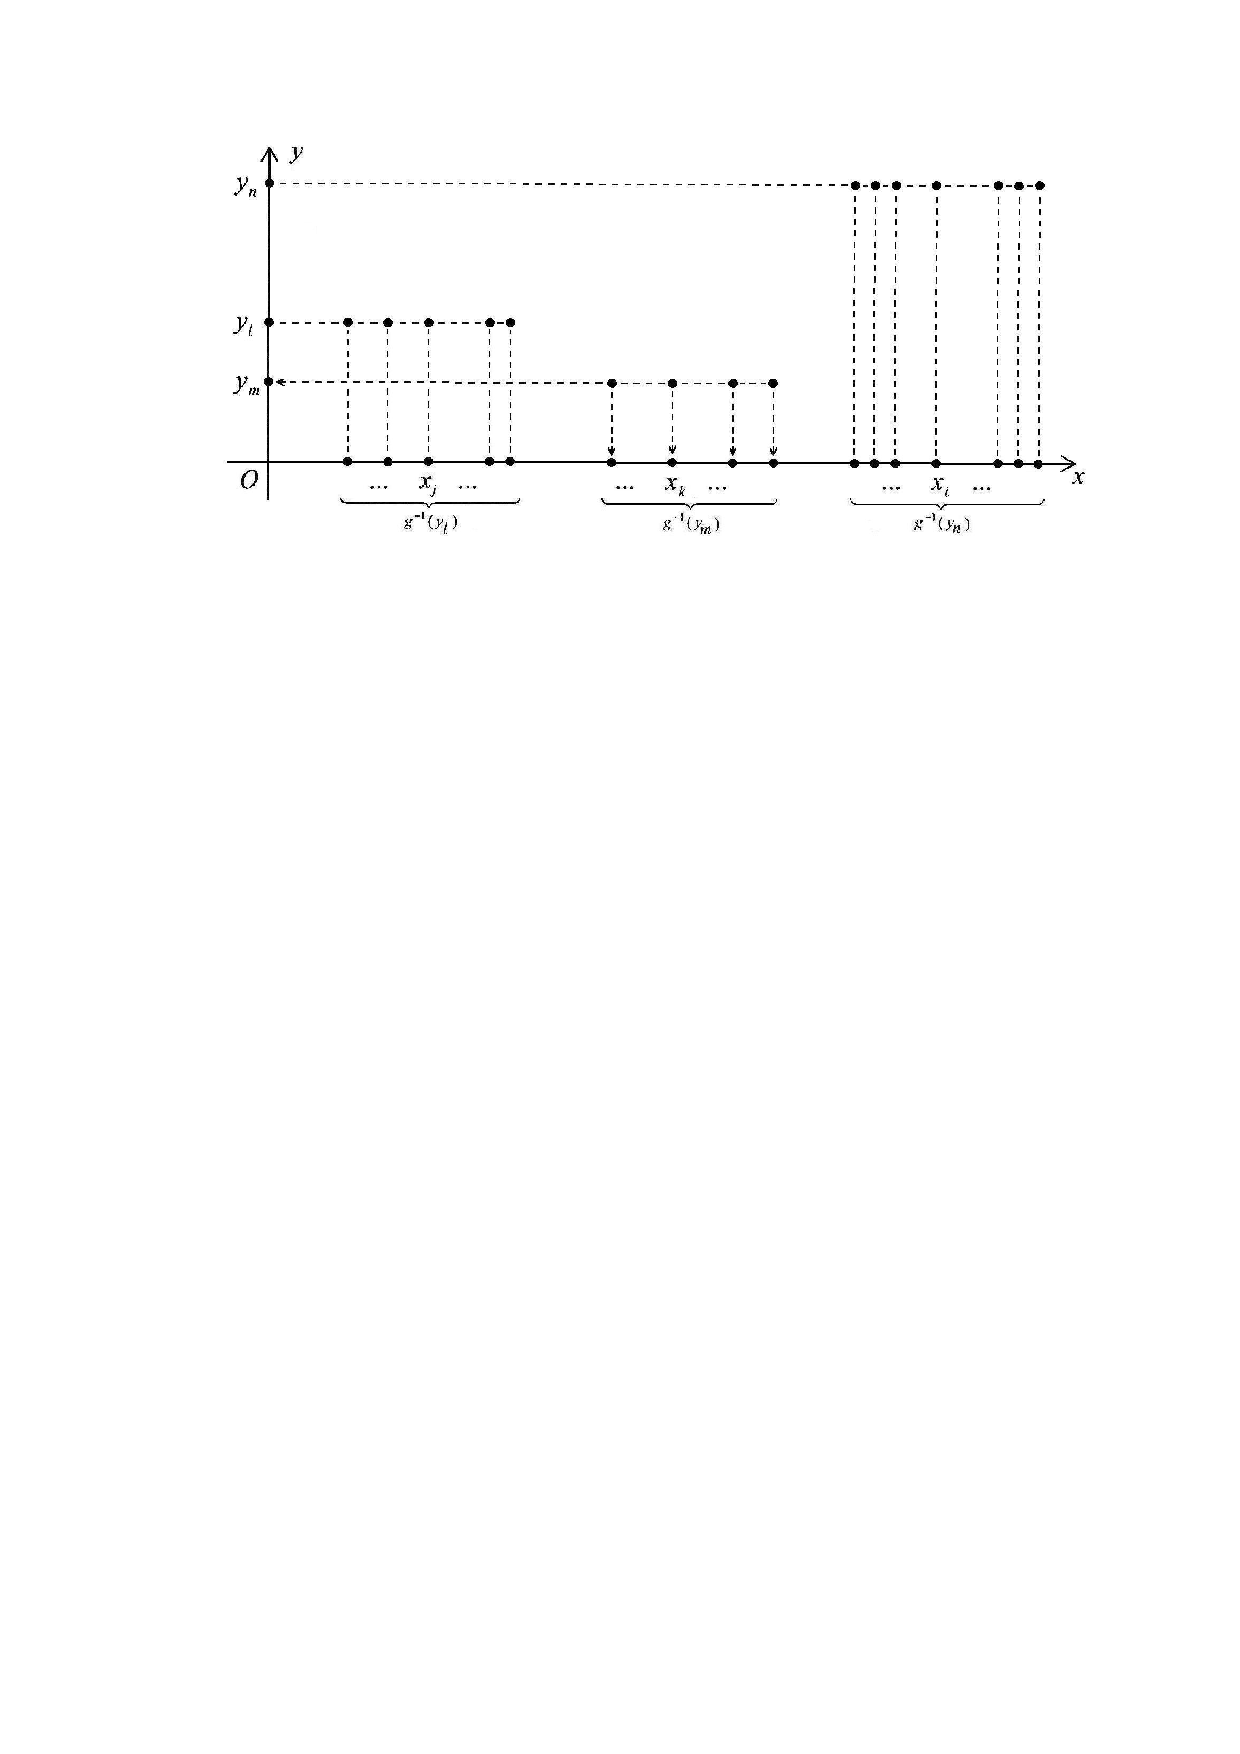
\includegraphics[]{pic/pic23}
	\caption{К доказательству теор. \ref{th:17.4}}
	\label{fig23}
\end{figure}
\begin{theorem}
\label{th:17.4}
\begin{enumerate}
	\item Для любой дискретной случайной величины $\xi$ и произвольной функции $g : \mathbb{R} \to \mathbb{R}$, математическое ожидание случайной величины $\eta = g(\xi)$ вычисляется по формуле
		\begin{equation*}
			\M\eta=\M g(\xi)=\sum_k g(x_k)p_k
		\end{equation*}
	\item Для любого абсолютно непрерывного случайного вектора
	$\xi = (\xi_1, \dots, \xi_n) \in \mathbb{R}^n$ и произвольной функции 
	$g : \mathbb{R} \to \mathbb{R}$, математическое ожидание случайной величины 
	$\eta = g(\xi)$ вычисляется по формуле
		\begin{equation*}
			\M\eta=\M g(\xi)=\int\limits_{-\infty}^{\infty}\ldots
			\int\limits_{-\infty}^{\infty}g(t_1,\ldots,t_n)f_{\xi_1,\ldots,\xi_n}(t_1,\ldots,t_n)dt_1\dots dt_n.
		\end{equation*}
\end{enumerate}

\end{theorem}

\begin{proof}
	Мы докажем эту теорему только для дискретного случая.
Пусть случайная величина $\xi$ принимает значения $x_1, x_2,\dots, x_k, \dots$ соответственно с вероятностями $p_1, p_2,\dots , p_k,\dots$ . Тогда $\eta= g(\xi)$ принимает
значения $y_1, y_2, \dots , y_m, \dots$ соответственно с вероятностями $q_1, q_2,\dots, q_m,\dots $, при этом полный прообраз $g^{−1}(y_m)$ может состоять из одного или более чем из одного элемента. Поэтому
	\begin{equation*}
		q_m=\P(g(\xi)=y_m)=\P(\xi\in g^{-1}(y_m))=\sum\limits
		{x_k\in g^{-1}(y_m)}p_k.
	\end{equation*}

	Тогда
	\begin{gather*}
	\M\eta=\M g(\xi)=\sum_m y_mq_m=\sum_m y_m \sum
	\limits_{x_k\in g^{-1}(y_m)} p_k=\\=
	\sum_m\sum\limits_{x_k\in g^{-1}(y_m)}g(x_k)p_k=\sum_kg(x_k)p_k.
	\end{gather*}
	Последнее равенство справедливо потому, что суммирование по $x_k\in g^{-1}(y_m)$ означает суммирование вдоль горизонтального уровня $y = y_m$ (см. рис. \ref{fig23}), суммирование по $m$ означает суммирование сумм на горизонтальных уровнях. Поэтому двойное суммирование в левой части эквивалентно суммированию по $k$ в правой части.
\end{proof}

\begin{theorem}
Математическое ожидание имеет следующие свойства.
\begin{enumerate}
	\item Если $C = const$, то $\M C = C$.
	\item Для любой случайной величины $\xi$ имеем $\M(\M\xi) = \M\xi$.
	\item Если $C = const$, то $\M(C\xi) = C\M\xi$.
	\item Для любой случайной величины $\xi$ имеем $|\M\xi| \leqslant \M|\xi|$. 
	\item Для любых случайных величин $\xi_1$ и $\xi_2$ имеем $\M(\xi_1 + \xi_2) = \M\xi_1 +\M\xi_2.$
	\item Если случайные величины $\xi_1$ и $\xi_2$ независимы, то $\M(\xi_1\xi_2) = \M\xi_1\M\xi_2$.
\end{enumerate}
\end{theorem}

\begin{proof}
	\begin{enumerate}
		\item Константу $C$ можно рассматривать как вырожденную случайную величину $\xi = C$, сосредоточенную в точке $x = C$. Её плотность есть $f_{\xi}(x)=\delta(x-C)$. Поэтому имеем $\M\xi^n=\M C^n=\int\limits^{\infty}_{\infty} x^n\delta(x-C)dx=C^n$ и, в частности $\M C=C$

		\item Т.к. $\M\xi=const$, то $\M(\M\xi)=\M\xi$.

		\item $\M(C\xi)^n=\int\limits^{\infty}_{-\infty}(Cx)^nf_{\xi}(x)dx=C^n\int\limits^{\infty}_{-\infty}x^nf_{\xi}(x)dx=C^n\M \xi^n$
		
		\item $|\M\xi^n|=|\int\limits^{\infty}_{-\infty}x^nf_{\xi}(x)dx|\leqslant\int\limits^{\infty}_{-\infty}|x^n|f_{\xi}(x)dx=
		\M|\xi|^n$ и, в частности, $|\M\xi|\leqslant\M|\xi|$.

		\item По теор. \ref{th:17.4} и \ref{th:15.7} имеем

			\begin{gather*}
				\M(\xi_1+\xi_2)=
				\int\limits^{\infty}_{-\infty}
				\int\limits^{\infty}_{-\infty}
				(x_1+x_2)
				f_{\xi_2,\xi_2}(x_1,x_2)dx_1dx_2
				=\\=
				\int\limits^{\infty}_{-\infty}
				x_1
				\left(\int\limits^{\infty}_{-\infty} 
				f_{\xi_2,\xi_2}(x_1,x_2)dx_1dx_2
				\right)
				+
				\int\limits^{\infty}_{-\infty}
				x_2
				\left(\int\limits^{\infty}_{-\infty} 
				f_{\xi_2,\xi_2}(x_1,x_2)dx_1dx_2
				\right)
				=\\=
				\int\limits^{\infty}_{-\infty}
				x_1 f_{\xi}(x_1)dx_1+
				\int\limits^{\infty}_{-\infty}
				x_2 f_{\xi}(x_2)dx_2=
				\M\xi_1+\M\xi_2.
			\end{gather*}
		\item По теор. \ref{th:17.4} и \ref{th:15.7} имеем

			\begin{gather*}
				\M(\xi_1\xi_2)=
				\int\limits^{\infty}_{-\infty}\int\limits^{\infty}_{-\infty}
				x_1x_2f_{\xi_2,\xi_2}(x_1,x_2)dx_1dx_2
				=\\=
				\int\limits^{\infty}_{-\infty}
				x_1f_{\xi_2,\xi_2}(x_1,x_2)dx_1 
				\int\limits^{\infty}_{-\infty}
				x_2f_{\xi_2,\xi_2}(x_1,x_2)dx_2=
				\M\xi_2\M\xi_2
			\end{gather*}
	\end{enumerate}
\end{proof}

\begin{zam}
	Обратное утверждение, к только что доказанному свойству 6), неверно. Следующий пример показывает, что из равенства $\M(\xi_1\xi_2)=\M\xi_2\M\xi_2$ не следует независимость величин $\xi_1$ и $\xi_2$.
\end{zam}
\begin{figure}[H]
	\centering
	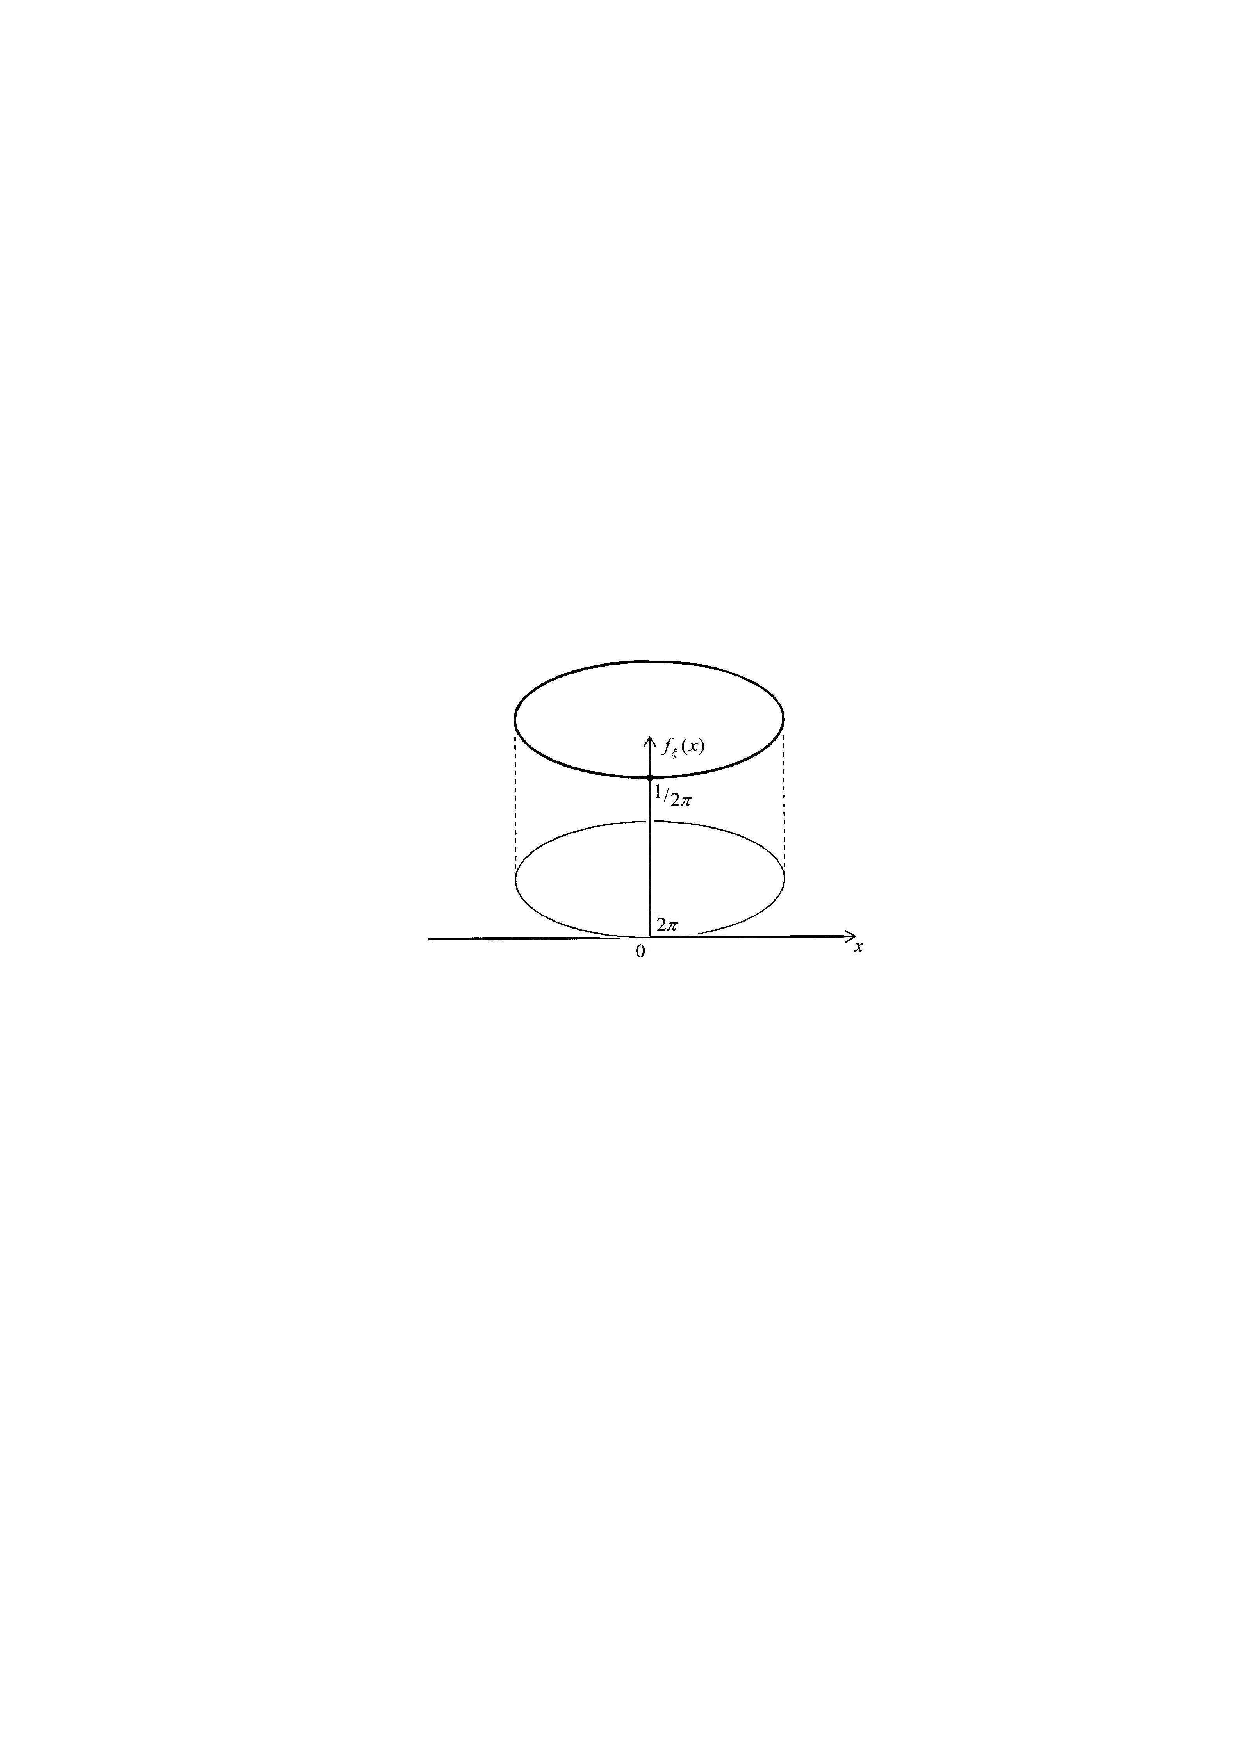
\includegraphics[]{pic/pic24}
	\caption{Равномерно распределённый угол.}
	\label{fig24}
\end{figure}

\begin{example}
	Пусть случайный угол $\phi$ равномерно распределён на окружности 
	$S^1 = \{z = e^{i\phi}\} \subset \mathbb{C} $, где $\phi\in [0, 2\pi]$. Её плотность
	\begin{equation*}
		f_{\phi}(x)=
		\begin{cases}
			\frac{1}{2\pi}, &\text{ если } x\in [0,2\pi]\\
			0, &\text{ если } x\notin [0,2\pi]\\
		\end{cases}
	\end{equation*}
	показана на рис. \ref{fig24}. Случайные величины $\xi_1 = \cos\phi$ и $\xi_2 = \sin\phi$ являются заведомо зависимыми. Ясно, что $\xi_2^2+\xi_1^2=1$. Однако математическое ожидание их произведения равно произведению их математических ожиданий.
	Действительно по теор. \ref{th:17.4} имеем

	\begin{gather*}
		\M\xi_1=\int\limits_0^{2\pi}\cos x\frac{1}{2\pi}dx=0 
		\\
		\M\xi_2=\int\limits_0^{2\pi}\sin x\frac{1}{2\pi}dx=0
		\\
		\M(\xi_1\xi_2)=\int\limits_0^{2\pi}\cos\sin x\frac{1}{2\pi}dx=0
	\end{gather*}
\end{example}%кирилл

\section{Дисперсия} 
%!TEX root = ../var.tex
\begin{definition}
1) Центральным моментом $n$-го порядка случайной
величины $\xi$ называется число
\begin{equation*}
\M(\xi − \M\xi)^n = \int_{-\infty}^{\infty}(x-\M\xi)^n f_{\xi}(x)dx
\end{equation*}

2) Дисперсией случайной величины $\xi$ называется центральный момент 2-го порядка, т.е. число
\begin{equation*}
\D\xi = \M(\xi − \M\xi)^2 = \int_{-\infty}^{\infty}(x-\M\xi)^2 f_{\xi}(x)dx.
\end{equation*}
\end{definition}

\begin{zam}
Для любой случайной величины $\xi$ её центральный момент 1-го порядка равен нулю, $\M(\xi − \M\xi) = \M\xi − \M\xi = 0$.
\end{zam}

\begin{zam}
Если ось $x$ рассматривать как тонкую металлическую проволоку с линейной плотностью массы $f_{\xi}(x)$, то дисперсия $\D\xi$ есть в точности момент инерции стержня относительно его центра тяжести $\M\xi$.
\end{zam}

\begin{lemma}
1) Для любой случайной величины $\xi$ имеем $\D\xi \geq 0$.

2) Если $C = const$, то $\D C = 0$.

3) Если $C = const$, то для любой случайной величины $\xi$ имеем $\D(C\xi) = C^2\D\xi.$
\end{lemma}
 
\begin{proof}

1) Т.к. $(x − \M\xi)^2 f_{\xi}(x) (x) \geq 0$, то интеграл в опред. 18.1.2) не меньше нуля.

2) $\D C = \M(C − \M C)^2 = 0$.

3) $\D(C\xi) = \M[C\xi −\M(C\xi)]^2 = \M[C(\xi −\M\xi)]^2 = C^2\M(\xi − \M\xi)^2 = C^2\D\xi.$

\end{proof}

\begin{zam}
Дисперсия (по прочтению формулы $\D\xi = \M(\xi − \M\xi)^2$)
равна <<среднему значению квадрата отклонения случайной величины от её среднего>>. То есть, дисперсия характеризует отклонение (разброс, кучность) значений случайной величины вокруг её среднего значения $\M\xi$.
В таком случае полезно следующее определение.	
\end{zam}

\begin{definition}
Число $\sigma = \sqrt{\D\xi}$ называется средне квадратическим отклонением случайной величины $\xi$.	
\end{definition}

\begin{theorem}
	Для любой случайной величины $\xi$ справедлива формула

\begin{equation*}
	\D\xi = \M\xi^2 − (\M\xi)^2 .
\end{equation*}

\end{theorem}

\begin{proof}

	\begin{gather*}
		\D\xi = \M(\xi − \M\xi)^2 = \M[\xi^2 − 2\xi \M\xi + (\M\xi)^2] =\\= \M\xi^2 − 2M(\xi \M\xi) + \M[(\M\xi)^2 ] =\\= \M\xi^2 − 2(\M\xi)^2 + (\M\xi)^2 = \M\xi^2 − (\M\xi)^2 .
	\end{gather*}

\end{proof}

\begin{theorem}
 Если случайные величины $\xi_1$ и $\xi_2$ независимы, то
$$\D(\xi_1 + \xi_2 ) = \D\xi_1 + \D\xi_2 .$$
 \end{theorem} 

\begin{proof}
 	\begin{gather*}
 		\D(\xi_1 + \xi_2 ) = \M(\xi_1 + \xi_2 )^2 − (\M(\xi_1 + \xi_2 ))^2 =\\= \M(\xi_1^2 + 2\xi_1 \xi_2 + \xi_2^2 ) - (\M\xi_1 + \M\xi_2 )^2 \stackrel{17.4.5)}{=}\\= \M\xi_1^2 + 2\M(\xi_1 \xi_2 ) + \M\xi_2^2 − (\M\xi_1)^2 − 2\M\xi_1 \M\xi_2 − (\M\xi_2 )^2  \stackrel{17.4.6)}{=}\\= \M\xi_1^2 − (\M\xi_1 )^2 + \M\xi_2^2 − (\M\xi_2 )^2 = \D\xi_1 + \D\xi_2 .
 	\end{gather*}
 \end{proof} 
 
\begin{example}
1) Пусть $\xi$ — подчиняется распределению Бернулли,
т.е. принимает два значения: 1 с вероятностью $p$ и 0 с вероятностью $q = 1 − p$, тогда 

\begin{gather*}
\M\xi = 1 \cdot p + 0 \cdot q = p,\quad
\M\xi^2 = 1^2 \cdot p + 0^2 \cdot q = p,\\
\D\xi = \M\xi^2 − (\M\xi)^2 = p − p^2 = pq.	
\end{gather*}

2) Вычислим математическое ожидание и дисперсию случайной величины $\xi$, имеющей биномиальное распределение, т.е. $\xi$ принимает значения $0, 1, 2, \ldots, n$ соответственно с вероятностями $\P(\xi_n = k) = C_n^k p^k (1 − p)^{n−k}$.
Возьмем $n$ независимых случайных величин $\xi_1 , \ldots, \xi_n$ имеющих одно и то же распределение Бернулли, т.е. с $\M\xi_i = p$ и $\D\xi_i = pq$ . Тогда их сумма $\xi = \xi_1 + \ldots + \xi_n$ имеет биномиальное распределение и

\begin{equation*}
\M\xi = \sum_{i=1}^{n}\M\xi_i = n\M\xi_1 = np, \quad
\D\xi = \D\xi_i = n\D\xi_1 = npq.		
\end{equation*}
\end{example}

% Рита

\section{Числовые характеристики зависимости
случайных величин} 
%!TEX root = ../var.tex
\begin{zam}
\label{zam:19.1}
	Мы знаем, что для независимых случайных величин
	дисперсия их суммы равна сумме их дисперсий
		\begin{equation*}
			\D(\xi_1+\xi_2)=\D \xi_2 +\D \xi_1
		\end{equation*}

	Чему равна дисперсия суммы в общем случае?
		\begin{gather*}
			\D(\xi_1+\xi_2)=\M(\xi_1+\xi_2)^2-[\M(\xi_1+\xi_2)]^2=\\=
			\M(\xi_1^2+\xi_2^2+2 \xi_1 \xi_2)-(\M \xi_1)^2 -(\M \xi_2)^2
			-2\M\xi_2\M\xi_2=\\=
			\D \xi_1+\D \xi_2+2[\M(\xi_1\xi_2)-\M \xi_1 \M \xi_2].
		\end{gather*}
	Если случайные величины $\xi_1$ и $\xi_2$ независимы, то по теор. 17.5.6. величина $\M(\xi_1\xi_2)−\M\xi_1\M\xi_2$ равна нулю. С другой стороны, из равенства её нулю вовсе не следует их независимость (см. пример 19.7). Поэтому эту величину можно использовать как <<индикатор степени зависимости>> случайных величин $\xi_1$ и $\xi_2$.
\end{zam}

\begin{definition}
	Ковариацией $\cov(\xi_1,\xi_2)$ случайных величин $\xi_2$ и
$\xi_2$ называется число
$$\cov(\xi_1,\xi_2)=\M[(\xi_1-\M \xi_2)(\xi_2-\M \xi_2)] $$
\end{definition}

\begin{lemma}
	Свойства ковариации
	\begin{enumerate}
		\item $\cov(\xi_1,\xi_2)=\M(\xi_1 \xi_2)-\M \xi_1 \M \xi_2$,
		\item $\cov(\xi,\xi)=\D \xi	$
		\item $\cov(\xi_1,\xi_2)=\cov(\xi_2,\xi_1)$
		\item $\cov(C \xi_1,\xi_2)=C\cov(\xi_1,\xi_2)$.
	\end{enumerate}
\end{lemma}

\begin{proof}
\hspace{0pt}
	\begin{enumerate}
		\item $\cov(\xi_1,\xi_2)=\M[(\xi_1-\M \xi_1)(\xi_2-\M \xi_2)]=\xi_1 \xi_2 - \xi_1\M \xi_2- \xi_2\M \xi_1+ \M \xi_1 \M \xi_2)
		=$ \newline $=\M(\xi_1 \xi_2)-\M(\xi_1)\M(\xi_2)$
		
		\item Следует из опред. 19.1
		\item Очевидно
		\item $\cov(C \xi_1,\xi_2)=\M(\xi_1 \xi_2)-\M(C\xi_1 \xi_2)-\M(C \xi_1)\M \xi_2=C[\M(\xi_1\xi_2)-\M \xi_1 \M \xi_2]$
	\end{enumerate}
\end{proof}

Пусть $\xi_1,\dots, \xi_n$ — случайные величины. Для сокращения формул обозначим через $\sigma_{ij}$ ковариацию $\cov(\xi_i, \xi_j)$, где $i, j \in \{1, \ldots, n\}.$

\begin{lemma}
	(О дисперсии линейной комбинации)

	Для любых случайных величин $\xi_1,\dots , \xi_n$ и любых чисел $c_1,\dots, c_n \in \mathbb{R}$ справедливо
	\begin{equation*}
		\D(c_1 \xi_1+\ldots+c_n \xi_n)=\sum_{i=1}^n\sum_{j=1}^n\sigma_{ij}c_ic_j.
	\end{equation*}
\end{lemma}

\begin{proof}
	Рассмотрим случайную величину $\eta = c_1 \xi_1 +\dots+ c_n \xi_n$.
	Нетрудно увидеть, что
	\begin{equation*}
		\eta-\M\eta=\sum_{i=1}^nc_i(\xi_i-\M \xi_i),
	\end{equation*}
	и что
	\begin{equation*}
		(\eta-\M\eta)^2=\sum_{i=1}^n\sum_{j=1}^nc_ic_j(\xi_i-\M \xi_i)(\xi_j-\M \xi_j).
	\end{equation*}
	Вычисляя математическое ожидание от обеих частей последнего равенства,
	получим требуемый результат.
\end{proof}

\begin{zam}\label{zam:19.5}
	Т.к. $\D\eta \geqslant 0$, то квадратичная форма $$\sum_{i=1}^n\sum_{j=1}^n\sigma_{ij}c_ic_j,$$ где $c_1,\dots, c_n \in \mathbb{R}$ рассматриваются как переменные, является неотрицательной. Из теории квадратичных форм известно, что все главные миноры матрицы неотрицательной квадратичной формы, в нашем случае матрицы
	\begin{equation*}
		(\sigma_{ij})=	
		\begin{pmatrix}
	  		\sigma_{11}& \sigma_{12}& \ldots & \sigma_{1n}\\
	  		\sigma_{21}& \sigma_{22}& \ldots & \sigma_{2n} \\
	  		\ldots & \ldots& \ldots & \ldots \\
	  		\sigma_{n1}& \sigma_{n2}& \ldots & \sigma_{nn}\\
		\end{pmatrix}
	\end{equation*}
	неотрицательны, и в частности, $\det\sigma_{ij} \geqslant 0$. При $n = 2$ это неравенство принимает вид
	\begin{equation*}
		\begin{vmatrix}
			\sigma_{11}& \sigma_{12}\\
		 	\sigma_{21}& \sigma_{22}\\
		\end{vmatrix}
		=
		\begin{vmatrix}
			\D \xi_1 & \cov{\xi_1 \xi_2}\\
			\cov{\xi_2 \xi_1} & \D \xi_2\\
		\end{vmatrix}
		=\D \xi_1 \D \xi_2-\cov^2(\xi_1, \xi_2)\geqslant 0		
	\end{equation*}
\end{zam}

\begin{zam}\label{zam:19.6}
Обсудим достоинства и недостатки ковариации, как
величины, характеризующей зависимость двух случайных величин.
\begin{enumerate}
	\item Если ковариация $\cov(\xi_1, \xi_2)$ отлична от нуля, то величины 
	$\xi_1$ и $\xi_2$ зависимы.
	
	\item Если ковариация $\cov(\xi_1, \xi_2)$ равна нулю, то зависимость случайных
	величин $\xi_1$ и $\xi_2$ приходится исследовать с помощью пп. 17.5 и 17.6.
	
	\item Самая сильная зависимость между случайными величинами — функциональная, а из функциональных — линейная зависимость, когда $\eta =
	a \xi + b$. Встречаются более слабые зависимости. Например, если по последовательности независимых случайных величин $\xi_1, \xi_2, \dots$построить случайные величины $\xi = \xi_1 +\dots + \xi_{32} + \xi_{33}$ и $\eta = \xi_{33} + \xi_{34}+\dots + \xi_{101}$, то эти
	величины зависимы, но очень <<слабо>> и лишь через одно-единственное общее слагаемое $\xi_{33}$. (Представьте себе, сильно ли зависимы число появлений
	орла в первых 33-х подбрасываниях монеты и число появлений орла в той
	же серии, но в испытаниях с 33-го по 101-е.)

	\item Ковариация не является <<безразмерной>>. Если $\xi$ — объём газа в сосуде, а $\eta$ — давление этого газа, то ковариация $\cov(\xi_1, \xi_2)$ измеряется в $ m^3 \cdot P $. При переходе к другой размерности, т.е. при умножении одной из величин $\xi, \eta$ на какое-нибудь число, ковариация тоже умножается на это число. Но умножение на число не сказывается на <<степени зависимости>> величин $\xi$ и $\eta$. Поэтому с физической точки зрения имеет смысл сравнивать зависимость случайных величин, ковариации которых имеют одну и ту же размерность.
	Из сказанного следует, что нужно как-то нормировать ковариацию,
	чтобы получить из неё безразмерную величину, абсолютное значение которой не менялось бы при умножении или сдвиге случайных величин на число и свидетельствовало бы о <<силе>> зависимости случайных величин.
	Такую величину доставляет следующее определение.
\end{enumerate}
\end{zam}

\begin{definition}
	Коэффициентом корреляции $\rho(\xi, \eta)$ случайных величин $\xi$ и $\eta$ называется число
	\begin{equation*}
		\rho(\xi,\eta)=\frac{\cov(\xi,\eta)}{\sqrt{\D\xi}\sqrt{\D\eta}}.
	\end{equation*}
\end{definition}
\begin{zam}\label{zam:19.8}
	Чтобы увидеть <<устройство>> коэффициента корреляции, распишем по определению величины, стоящие в числителе и знаменателе
	\begin{equation*}
		\rho(\xi, \eta)=\frac{\M[(\xi-\M \xi)(\eta-\M\eta)]}
		{\sqrt{\M(\xi-\M)^2}\sqrt{\M(\eta-\M\eta)^2}}.
	\end{equation*}
		Для физиков уместно провести аналогию формулы косинуса угла между
	векторами в евклидовом пространстве и формулой коэффициента корреляции.
	
	Во-первых, так как для любых случайных величин 
	$\xi, \eta : \Omega \to \mathbb{R}$ определена их сумма 
	$(\xi +\eta)(x) = \xi(x)+\eta(x)$ и умножение любой случайной величины на число 
	$(\alpha \cdot \xi)(x) = \alpha \cdot \xi(x)$, где $\alpha \in \mathbb{R}$, то эти операции превращают
	множество $\{\xi : \Omega \to \mathbb{R}\}$ всех случайных величин в линейное (векторное)	пространство.
	
	Во-вторых, в этом пространстве ковариация $\cov(\xi, \eta)$ является скалярным произведением двух <<векторов>> $\xi$ и $\eta$ и превращает его в евклидово.

	И в-третьих, <<длиной>> случайной величины $\xi$ является её среднеквадратичное отклонение, которая равна корню из скалярного произведения <<вектора>> $\xi$ самого на себя
	$\sqrt{\cov(\xi, \xi)}=\sqrt{\D\xi}$. Поэтому коэффициент корреляции есть косинус угла между случайными величинами $\xi$ и $\eta$ в пространстве случайных величин. Надо только доказать, что $−1 \leqslant \rho(\xi, \eta) \leqslant 1$. Заметим, что т.к. пространство случайных величин бесконечномерное, то рисовать в виде векторов можно только те случайные величины, которые	в фиксированном базисе представимы в виде конечных линейных комбинаций элементов этого базиса.
\end{zam}

\begin{definition}
	Случайные величины $\xi$ и $\eta$ называются некоррелированными, если $\rho(\xi, \eta) = 0$. (Некоррелированность является аналогом
ортогональности.)
\end{definition}

\begin{theorem}[Свойства коэффициента корреляции]
	Свойства:
	\begin{enumerate}
		\item Если случайные величины $\xi$ и $\eta$ независимы, то $\rho(\xi, \eta) = cov(\xi, \eta) =0.$
		\item $|\rho(\xi, \eta)| ≤ 1$.
		\item $|\rho(\xi, \eta)| = 1$ тогда и только тогда, когда случайные величины $\xi$ и $\eta$ линейно зависимы, т.е. существуют числа $a, b \in \mathbb{R} $и $a \neq 0$, такие что $\xi = a\eta + b$.
	\end{enumerate}
\end{theorem}

\begin{proof}
	\begin{enumerate}
		\item Косвенно мы уже это доказали, см. пп. 19.5.6) и 19.3.1).
		\item Требуемое неравенство следует из неравенства $\D\xi_1\D\xi_2−\cov^2(\xi_1, \xi_2) \geqslant 0$, доказанного в п. 19.5.
		\item Докажем сначала, что из $|\rho(\xi, \eta)|$ = 1 следует, что $\xi = a\eta + b$. Перепишем опред. 19.7 в виде
		\begin{equation*}
			\rho(\xi, \eta) =\M\left(\frac{\xi-\M \xi}{\sqrt{\D \xi}}\cdot
			\frac{\eta-\M\eta}{\sqrt{\D\eta}} \right).
		\end{equation*}
		Рассмотрим сначала случай $\rho(\xi, \eta) = +1$. Воспользуемся неравенством
		$\alpha \beta\leqslant \frac{1}{2}(\alpha^2 + \beta^2)$
		\begin{gather*}
			\rho(\xi, \eta) =\M\left(
			\frac{\xi-\M \xi}{\sqrt{\D \xi}}
			\cdot
			\frac{\eta-\M\eta}{\sqrt{\D\eta}} 
			\right)
			\leqslant\\\leqslant
			\frac{1}{2}\M
			\left[ 
			\left(\frac{\xi-\M \xi}{\sqrt{\D \xi}}\right)^2
			+
			\left(\frac{\eta-\M\eta}{\sqrt{\D\eta}}\right)^2
			\right]
			=\frac{1}{2}\cdot2=1
		\end{gather*}
		Т.к $\rho(\xi, \eta) = +1$, то последнее неравенство переходит в равенство
		\begin{equation*}
			\M\left(\frac{\xi-\M \xi}{\sqrt{\D \xi}}\cdot
			\frac{\eta-\M\eta}{\sqrt{\D\eta}} \right)=
			\frac{1}{2}\M
			\left[ 
			\left(\frac{\xi-\M \xi}{\sqrt{\D \xi}}\right)^2
			+
			\left(\frac{\eta-\M\eta}{\sqrt{\D\eta}}\right)^2
			\right]
		\end{equation*}
		которое можно переписать в виде
		\begin{equation*}
			\M\left(
			\frac{\eta-\M\eta}{\sqrt{\D\eta}}-\frac{\xi-\M \xi}{\sqrt{\D\xi}} 
			\right)^2=0
		\end{equation*}
		или в виде
		\begin{equation*}
			\M\left(\xi-\frac{\sqrt{\D \xi}}{\sqrt{\D \eta}}\eta-\M \xi+
			\frac{\sqrt{\D \xi}\M\eta}{\sqrt{\D \eta}}
			\right)^2=0
		\end{equation*}
		Обозначим $a\frac{\sqrt{\D\xi}}{\sqrt{\D\eta}}$ и $b=\frac{\sqrt{\D \xi}\M\eta}{\sqrt{\D \eta}}$, получим
		\begin{equation*}
			\M(\xi-a \eta-b)^2=0
		\end{equation*}
		По определению математического ожидания равенство нулю математического ожидания неотрицательной случайной величины означает, что эта величина равна нулю, поэтому $\xi = a\eta + b$.

		В случае $\rho(\xi, \eta) = −1$ воспользуемся неравенством $\alpha\beta \geq −\frac{1}{2}(\alpha^2 + \beta^2)$ и по аналогии из неравенства
		\begin{gather*}
			\rho=\M\left(
			\frac{\xi-\M \xi}{\sqrt{\D \xi}}
			\cdot
			\frac{\eta-\M\eta}{\sqrt{\D\eta}} 
			\right)
			\leqslant\\\leqslant
			\frac{1}{2}\M
			\left[ 
			\left(\frac{\xi-\M \xi}{\sqrt{\D \xi}}\right)^2
			+
			\left[ \left(\frac{\eta-\M\eta}{\sqrt{\D\eta}}\right)^2
			\right]\right]
			=\frac{1}{2}\cdot2=-1
		\end{gather*}
		получим требуемый результат.

		Докажем теперь, что из $\eta = a\xi + b$ следует, что $|\rho	(\xi, \eta)| = 1$. Вопользуемся свойствами математического ожидания и дисперсии.
		\begin{gather*}
			\rho(\xi,a\xi+b)=
			\M
			\left(
			\frac{\xi-\M\xi}{\sqrt{\D\xi}}
			\cdot
			\frac{a\xi+b-\M (a\xi+b)}{\sqrt{\D( a\xi+b)}}
			\right)
			=\\=
			\M\left(
			\frac{\xi-\M \xi}{\sqrt{\D\xi}}\cdot
			\frac{a\xi+b-\M (a\xi+b)}{\sqrt{\D (a\xi+b)}} 
			\right)=
			\M\left(
			\frac{\xi-\M \xi}{\sqrt{\D\xi}}\cdot
			\frac{a\xi-\M (a\xi)}{\sqrt{\D (a\xi)}} 
			\right)=\\=
			a\M\left(
			\frac{(\xi-\M\xi)^2}{\sqrt{\D\xi\D(a\xi)}}
			\right)=
			\frac{a\M(\xi-\M\xi)^2}{\sqrt{a^2\D^2\xi}}
			=\frac{a}{|a|}=
			\left\{
			\begin{aligned}
				&1, &\text{ если } a>0\\
				&-1, &\text{ если } a<0	
			\end{aligned}
			\right.
		\end{gather*}
	\end{enumerate}
\end{proof}

\begin{definition}
	Если $\rho(\xi, \eta) < 0$, то случайные величины $\xi$ и $\eta$
называются отрицательно коррелированными; если $\rho(\xi, \eta) > 0$, то — положительно коррелированными.
\end{definition}
\begin{zam}\label{zam:19.12}
Смысл знака коэффициента корреляции особенно ясен
в случае $\rho(\xi, \eta) = \pm 1$. В этом случае знак $\rho$ совпадает со знаком $a$ в равенстве $\eta = a\xi + b$. Значение $\rho(\xi, \eta) = 1$ означает, что чем больше $\xi$, тем больше и $\eta$. Напротив, $\rho(\xi, \eta) = −1$ означает, что чем больше $\xi$, тем меньше и $\eta$. Аналогично можно трактовать знак коэффициента корреляции и
в случае, когда $|\rho(\xi, \eta)| < 1$, помня при этом, что зависимость случайных
величин $\xi$ и $\eta$ не линейная и может быть даже не функциональная.
\end{zam}
\begin{num}	
	Найти коэффициент корреляции между числом выпадений единицы и числом выпадений шестёрки при n подбрасываниях игральной кости.

Решение.

 Для $i = 1, 2, 3, 4, 5, 6$ обозначим через $\xi_i$ случайную величину,
равную числу выпадений грани с $i$ очками при $n$ подбрасываниях кости. Посчитаем сначала ковариацию $\cov(\xi_1, \xi_6)$ = $\M(\xi_1\xi_6) − \M\xi_1\M\xi_6$.
Каждая из случайных величин $\xi_i$ имеет биномиальное распределение и
каждое из её значений может появиться в каждом из $n$ подбрасываниях с
вероятностью $p = 1/6$, и по п. 19.9.2) $\M\xi_i = np = n/6$ и $\D\xi_i = npq = 5n/36$.

Т.к. при каждом подбрасывании выпадает какая-то грань, то $\xi_1+\dots +\xi_6 = n.$ Т.к. игральная кость симметрична, то при $i\neq j$ все математические ожидания $\M(\xi_i\xi_j)$ одинаковы. Заметим, что из той же симметрии следует, что $\M(\xi_i\xi_i)$ то же одинаковы и равны $\M^2\xi_i = \D\xi_i + (\M\xi_i)^2 =
5n/36 + n^2/36 = (n^2 + 5n)/36.$

Подсчитаем величину $\M[\xi_1(\xi_1 +\dots + \xi_6)]$ двумя способами. Во-первых,
она равна
\begin{equation*}
	\M[\xi_1(\xi_1 + \dots+ \xi_6)] = \M(\xi_1\cdot n) = n^2/6,
\end{equation*}
а во-вторых,
\begin{equation*}
	\M[\xi_1(\xi_1 +\dots + \xi_66)] = \M\xi^2_1 + 5\M(\xi_1\xi_6) = (n^2 + 5n)/36 + 5M(\xi_1\xi_6).
\end{equation*}

Отсюда $5M(\xi_1\xi_6)=n2/6 − (n2 + 5n)/36,$т.е
\begin{equation*}
\M(\xi_1\xi_6)=\frac{n^2-n}{36} 	
\end{equation*} 
Следовательно, искомый коэффициент корреляции равен
\begin{equation*}
	\rho(\xi_1,\xi_2)=\frac{\cov(\xi_1,\xi_6)}{\sqrt{\D\xi_1}\sqrt{\D\xi_6}}=
	\frac{\M(\xi_1,\xi_6)-\M(\xi_1)\M(\xi_6)}{\sqrt{\D\xi_1}\sqrt{\D\xi_6}}=
	\frac{(n^2 − n)/36 − n^2/36}{5n/36}=-\frac{1}{5}
\end{equation*}
Естественно, что коэффициент корреляции не зависит от числа подбрасываний игральной кости.
	
\end{num}% кирилл

%%%%%%%%%%%%%%%%%%%%%%
\part{Законы больших чисел}
%%%%%%%%%%%%%%%%%%%%%%

\section{Неравенство Бьенеме–Чебышёва и
неравенство Маркова}
%!TEX root = ../var.tex
Напомним, что мы рассматриваем случайные величины, имеющие конечные начальные и центральные моменты до $n$-го порядка включительно.
Метод доказательства неравенств, изучаемых в этом параграфе, принадлежит Чебышёву\footnote{
Чебышёв, Пафнутий Львович (распространено неправильное произношение его фамилии с ударением на первый слог) (1821 — 1894), выдающийся русский математик и механик, внёсший большой вклад
в теорию вероятностей, теорию приближений, теорию интерполирования функций, интегральное исчисление и картографию. Работая на <<оборонку>>, он улучшил дальнобойность и точность артиллерийской
стрельбы, чем оказал большое влияние на развитие русской артиллерии.	
}.

\begin{theorem}[Неравенство Маркова\footnote{
	Марков, Андрей Андреевич (1856 — 1922), выдающийся русский математик, внёсший большой вклад
в теорию вероятностей и математический анализ.
} , 1913 г.]

 Для любой случайной
величины $\xi$ и для любого $\epsilon \in (0, \infty)$, имеет место неравенство

\begin{equation*}
\P( |\xi| \geq \epsilon ) \leq \frac{\M|\xi|}{\epsilon}	
\end{equation*}	
\end{theorem}

\begin{proof}
	Если $c$ -- плотность случайной величины $\xi$, то

\begin{equation*}
	\P( |\xi| \geq \epsilon ) = \int\limits_{|x|\geq \epsilon} f_{\xi}(t)dt
\end{equation*}

Ясно, что для всех $t \in \{ |x| \geq \epsilon \}$ выполнено неравенство $\frac{|t|}{\epsilon} \geq 1$. Поэтому при замене $f_{\xi}(t)$ на $\frac{|t|}{\epsilon} f_{\xi}(t)$ подынтегральное выражение не уменьшится, т.е.

\begin{equation*}
\P( |\xi| \geq \epsilon ) = \int\limits_{|x| \geq \epsilon}f_{\xi}(t)dt \leq \int\limits_{|x| \geq \epsilon} \frac{|t|}{\epsilon} f_{\xi}(t)dt = \frac{1}{\epsilon}\int\limits_{|x| \geq \epsilon} |t|f_{\xi}(t)dt. 
\end{equation*}

Если теперь мы увеличим область интегрирования с ${ |x| \geq \epsilon }$ до $(−\infty, \infty)$,
то интеграл справа тоже не уменьшится. Окончательно получаем

\begin{equation*}
	\P( |\xi| \geq \epsilon ) \leq \frac{1}{\epsilon} \int\limits_{|x| \geq \epsilon} |t|f_{\xi}(t)dt \leq \frac{1}{\epsilon} \int\limits_{-\infty}^{\infty} |t|f_{\xi}(t)dt = \frac{\M|\xi|}{\epsilon}
\epsilon
\end{equation*}
\end{proof}


\begin{consq}[Двойственное неравенство Маркова]
	Для любой случайной величины $\xi$ и для любого $\epsilon \in (0, \infty)$ имеет место неравенство
$$\P( |\xi| < \epsilon ) \geq 1 − \frac{\M|\xi|}{\epsilon}$$
\end{consq}

\begin{proof}
 	По лемме 3.7 имеем $\P( |\xi| < \epsilon ) = 1 − \P( |\xi| \geq \epsilon ) $. Подставим это выражение в неравенство Маркова, получим требуемый результат.
 \end{proof} 

\begin{theorem}[Обобщённое неравенство Маркова]
 Для любой случайной величины $\xi$, для любого $\epsilon \in (0, \infty)$ и любой монотонно возрастающей
функции $g : (0, \infty) \to (0, \infty)$ имеет место неравенство
$\P( |\xi| \geq \epsilon ) \leq \frac{\M g(|\xi|)}{g(\epsilon)}$
 \end{theorem} 
 
 \begin{proof}
 	Поскольку функция $g$ монотонно возрастает, то
$\P( |\xi| \geq \epsilon ) = \P( g(|\xi|) \geq g(\epsilon) )$. Оценивая последнюю вероятность согласно неравенству Маркова, получим требуемый результат:

\begin{equation*}
	\P(g(|\xi|) \geq g(\epsilon)) \leq \frac{\M g(|\xi|)}{g(\epsilon)}
\end{equation*}
 \end{proof}
 
 \begin{consq}
Для любой случайной величины $\xi$, для любого $\epsilon \in (0, \infty)$, и любой монотонно возрастающей функции $g : (0, \infty) \to (0, \infty)$ имеет место неравенство

\begin{equation*}
	\P(|\xi - \M\xi| \geq) \leq \frac{\D\xi}{\epsilon^2}
\end{equation*}
(двойственное к обобщённому неравенству Маркова).
Доказательство аналогично доказательству след. 20.2.
В 1853 г. И.-Ж. Бьенеме\footnote{
	И.-Ж. Бьенеме (Irenee-Jules Biemayme, 1796 — 1878), французский математик, основные работы по теории вероятностей и математической статистике.} 
и в 1866 г. независимо от него П.Л. Чебышёв
доказали следующее неравенство. 	
 \end{consq}

\begin{theorem}[Неравенство Бьенеме – Чебышёва]
Для любой случайной величины $\xi$ и любого $\epsilon \in (0, \infty)$ имеет место неравенство
$$\P( |\xi − \M\xi| \geq \epsilon ) \leq \frac{\D\xi}{\epsilon^2}$$
\end{theorem}

\begin{proof}
Т.к. неравенство Маркова 20.1 справедливо для произвольной случайной величины, то перепишем его для случайной величины $\xi − \M\xi$, получим 

\begin{equation*}
	\P( |\xi − \M\xi| \geq \epsilon ) \leq \frac{\M|\xi - \M\xi|^2}{\epsilon}
\end{equation*}

Зададим функцию $g : (0, \infty) \to (0, \infty)$ по формуле $g(\epsilon) = \epsilon^2$. Видно,
что она является монотонно возрастающей и поэтому удовлетворяет условиям теор. 20.3, и следовательно, для неё выполнено обобщённое неравенство Маркова
$$\P( |\xi − \M\xi| \geq \epsilon ) \leq \frac{\M(\xi - \M\xi)^2}{\epsilon^2} = \frac{\D\xi}{\epsilon^2} $$
\end{proof}

\begin{consq}
Для любой случайной величины $\xi$ и любого $\epsilon \in (0, \infty)$, имеет место неравенство
$$\P( |\xi − \M\xi| < \epsilon ) \geq 1 − \frac{\D\xi}{\epsilon^2}$$
(двойственное к неравенству Бьенеме – Чебышёва).
Мы будем называть двойственное неравенство тоже неравенством Бьенеме – Чебышёва.
\end{consq}

\begin{consq}
Для любой случайной величины $\xi$ вероятность того,
что она примет значение, отличающееся от её среднего $\M\xi$ более чем на три корня из её дисперсии, не превосходит $\frac{1}{9}$, т.е.
$$\P(|\xi - \M\xi| \geq 3\sqrt{\D\xi}) \leq \frac{1}{9}$$
\end{consq}

\begin{proof}
Из неравенства Бьенеме-Чебышёва имеем
$$ \P(|\xi − \M\xi| \geq 3\sqrt{\D\xi}) \leq \frac{\D\xi}{(3\sqrt{\D\xi})^2} = \frac{1}{9}$$
 \end{proof} %Рита

\section{Последовательности случайных величин}
%!TEX root = ../var.tex
\begin{zam}
\label{zam:21.1}
Напомним, что по определению \ref{def:11.1} случайная величина
есть функция $ \xi : \omega \to R$. Поdэтому последовательность случайных величин
$$\xi_1, \xi_2,\dots, \xi_n,\dots = \{\xi_n\}_{n=1}^{\infty}\equiv\{\xi_n\}$$
есть на самом деле последовательность функций $\{\xi_n : \omega \to R\}_{n=1}^{\infty}$, определённая на одном и том же пространстве элементарных событий $\omega$.
\end{zam}
В математическом анализе мы изучили следующие две сходимости по-
следовательности функций.

\begin{definition}
\label{def:21.2}
	Последовательность функций $\xi_1, \xi_2,\dots , \xi_n,\dots$ сходится к функции $\xi$ поточечно, если для любой точки $\omega \in \omega$ последовательность чисел (значений) $\xi_1(\omega), \xi_2(\omega),\dots, \xi_n(\omega),\dots$ сходится к значению $\xi(\omega)$ функции $\xi$; или короче\footnote{Используя определение сходимости числовой последовательности.} $\lim\limits_{n\to\infty}\xi_n(\omega) = \xi(\omega)$
	для любой точки $\omega \in \omega$.
\end{definition}

\begin{definition}
\label{def:21.3}
	Последовательность функций $\xi_1, \xi_2,\dots, \xi_n,\dots$ сходится к функции $\xi$ поточечно почти всюду в $\Omega$, если подмножество $A \subset
\Omega$, в которых поточечная сходимость не выполняется, имеет меру 0, т.е.
$\mu(A) = 0$.
В теории вероятностей объекты $\omega, A, \Omega$ являются событиями, а мерой
их наступления является вероятность, поэтому в теории вероятностей
сходимости <<почти всюду>> соответствует так называемая сходимость
<<почти наверное.>>
\end{definition}

\begin{definition}
\label{def:21.4}
	Говорят, что последовательность случайных величин $\{\xi_n\}$ сходится почти наверное к случайной величине $\xi$, если имеют
место эквивалентные друг другу равенства
\begin{gather*}
	P\left\{\omega\in\Omega| \lim\limits_{n\to\infty}\xi_n(\omega)=\xi(\omega) \right\}=1 \\
	\text{и} \\
	P\left\{\omega\in\Omega| \lim\limits_{n\to\infty}\xi_n(\omega)\neq\xi(\omega) \right\}=0
\end{gather*}
\end{definition}
\begin{zam}
\label{zam:21.5}
Чтобы пользоваться на практике сходимостью <<почти наверное>> необходимо знать, как устроены отображения $\omega \mapsto \xi_n(\omega)$.
Как правило в задачах теории вероятностей известны не сами случайные
величины $\xi_n$, а их функции распределения, скажем $P(\xi_n \leqslant x) = F_{\xi_n}(x) =\int\limits_{-\infty}{x}f_{\xi_n}(t)dt$. Можно ли в таком случае, обладая информацией только о функциях распределения, каким-нибудь образом исследовать сходимость последовательности случайных величин $\{\xi_n\}$? Ответ: да, можно, если потребовать, чтобы вероятность тех элементарных исходов $\omega$, для которых значение $\xi_n(\omega)$ не попадает в <<$\epsilon$-окрестность>> числа $\xi(\omega)$, сходилась к нулю при $n \to \infty$. В теории вероятностей эту идею реализуют с помощью так называемой <<сходимости по вероятности>>.
\end{zam}

\begin{definition}
\label{def:21.6}
	Говорят, что последовательность случайных величин $\{\xi_n\}$ сходится по вероятности к случайной величине $\xi$, если для любого
$\varepsilon \in (0,\infty)$ имеют место эквивалентные равенства
\begin{gather*}
	\lim_{n\to\infty}P(|\xi_n- \xi|\geqslant \varepsilon)=0 \\
	\lim_{n\to\infty}P(|\xi_n- \xi|\leqslant \varepsilon)=1 \tag{*}
\end{gather*}

\end{definition}

Если ${\xi_n}$ сходится по вероятности к $\xi$, то вместо пределов (\ref{def:21.6}) коротко пишут <<$\xi_n\stackrel{P}{\to} \xi$ при $n \to \infty,$>> а т.к. $n \to \infty$ всегда, то ещё короче: <<$\xi_n\stackrel{P}{\to} \xi$.>>

Хотя на практике для проверки такой сходимости проверяют выполнение
одного из равенств (\ref{def:21.6}).

\begin{repdefinition}[Пример]
Рассмотрим последовательность случайных величин $\{\xi_n\}$ в которой для каждого n случайная величина задана следующим рядом распределения
\begin{center}
	\begin{tabular}{|c|c|c|}
	\hline
	$\xi_n$ & $c$& $n^3$\\ \hline
	$P$ & $1-1/n$& $1/n$\\ \hline
	\end{tabular}	
\end{center}

	Докажем, что эта последовательность сходится по вероятности к вырожденной случайной (детерминированной) величине $\xi$, имеющей ряд распределения
	\begin{tabular}{|c|c|}
	\hline
	$\xi$ & $0$\\ \hline
	$P$ & $1$\\ \hline
	\end{tabular}, а проще говоря, сходится по вероятности к нулю.

	Действительно, зафиксируем произвольное $\varepsilon > 0$. Для всех $n$, начиная
с некоторого $n_0$ такого, что $n^3_0>\varepsilon$, выполнено равенство
\begin{equation*}
	P(|\xi_n-0|\geqslant\varepsilon)=P(\xi_n\geqslant\epsilon)=P(\xi_n=n^3)=\frac{1}{n}.
\end{equation*}
Применяя теперь определение \ref{def:21.6} получаем
\begin{equation*}
	\lim\limits_{n\to\infty} P(|\xi_n-0|\geqslant\epsilon)=\lim\limits_{n\to\infty}\frac{1}{n}=0
\end{equation*}
т.е. последовательность случайных величин $\xi_1, \xi_2, \dots , \xi_n, \dots $сходится по вероятности к $\xi$, т.е. $\xi_n \stackrel{P}{\to}\xi$.

В нашем примере случайные величины $\xi_n$ с ростом $n$ могут принимать
всё бoльшие и бoльшие значения, но с всё меньшей и меньшей вероятностью.
\end{repdefinition}


\begin{zam}
\label{zam:21.7}
Сходимость по вероятности может не сопровождаться сходимостью математических ожиданий (или других начальных и
центральных моментов): 
из $\xi_n\stackrel{P}{\to} \xi$ не следует, что $\M\xi_n \to \M\xi$. Например,
в предыдущем примере $\xi_n
\stackrel{P}{\to} \xi$, однако $\M\xi_n^2 = n2$ и $\M\xi = 0$, и ясно, что
последовательность $1, 4, 9, \dots$ не сходится к нулю.
Сходимость по вероятности обладает теми же свойствами, как и поточечная сходимость.
\end{zam}

\begin{theorem}[Без доказательства]
\label{th:21.8}
	Если $\xi_n \stackrel{P}{\to} \xi$ и $\eta_n\stackrel{P}{\to} \eta$, то
	\begin{enumerate}
		\item  $\xi_n + \eta_n\stackrel{P}{\to} \xi + \eta$,
		\item $\xi_n \cdot \eta_n\stackrel{P}{\to} \xi \cdot \eta$,
		\item Если $g$ — непрерывная функция, то $g(\xi_n) \stackrel{P}{\to} g(\xi)$.
		\item Если $\xi_n \stackrel{P}{\to} C$ и функция g непрерывна в точке C, то $g(\xi_n) \stackrel{P}{\to} g(C)$.
	\end{enumerate}
\end{theorem}

Другой тип сходимости случайных величин, который нам понадобится
в дальнейшем, определяется через поточечную сходимость функций распределений. Это так называемая <<слабая сходимость.>> Пусть задана последовательность случайных величин $\{\xi_n\}_{n=1}^{\infty}$ с функциями распределения $\{F_{\xi_n}(x)\}_{n=1}^{\infty}$, и задана случайная величина $\xi$ с функцией распределения $F_\xi(x)$.

\begin{definition}
\label{def:21.9}
	Говорят, что последовательность случайных величин $\{\xi_n\}_{n=1}^{\infty}$ слабо сходится к случайной величине $\xi$, если последовательность их функций распределения $\{F_{\xi_n}(x)\}^{\infty}_{n=1}$ сходится поточечно к функции распределения $F_\xi(x)$, т.е. $\lim\limits_{n\to\infty}
	F_{\xi_n}(x) = F_\xi(x)$.

Если $\{\xi_n\}$ слабо сходится к $\xi$, то коротко пишут $\xi_n \Rightarrow \xi$. На практике для проверки слабой сходимости проверяют выполнение равенства
$$\lim \limits_{n\to\infty} F_{\xi_n}(x) = F_\xi(x)$$ для любого $x \in \mathbb{R}$.
\end{definition}

\begin{theorem}
\label{th:21.10}
	\hspace{0pt}
	\begin{enumerate}
		\item Если $\xi_n\stackrel{P}{\to}\xi,$ то $\xi_n\Rightarrow\xi$
		\item Если $\xi_n\Rightarrow C=const$, то $\xi_n \stackrel{P}{\to} C$
		\item Если $\xi_n\stackrel{P}{\to} C$ и $\eta_n\Rightarrow\eta$, то $\xi_n\cdot\eta_n\Rightarrow C\eta$
		\item Если $\xi_n\stackrel{P}{\to} C$ и $\eta_n\Rightarrow\eta$, то $\xi_n+\eta_n\Rightarrow C+\eta$
	\end{enumerate}
\end{theorem}% Кирилл


\section{Законы больших чисел} 
%!TEX root = ../var.tex
Одним из главных разделов теории вероятностей составляют так называемые <<предельные теоремы>>. Они описывают условия возникновения вероятностных закономерностей при наличии большого числа случайных факторов. 

Предельные теоремы можно условно разделить на три типа:
1) закон больших чисел, 2) предельные теоремы биномиального распределения и 3) центральные предельные теоремы. 

Этот и следующие параграфы посвящены изучению таких теорем.

\begin{definition}
Говорят, что последовательность случайных величин $\{\xi_n\}^\infty_{n=1}$ удовлетворяет закону больших чисел (ЗБЧ), если для любого $\epsilon \in (0, \infty)$ (при некоторых дополнительных условиях) имеют место эквивалентные друг другу равенства
\end{definition}

\begin{equation}
	\label{lim1}
	\lim\limits_{n\to\infty}
	\P\left(\left|
		\frac{1}{n}\sum\limits_{k=1}^n \xi_k-
		\frac{1}{n}\sum\limits_{k=1}^n \M\xi_k
	\right|<\epsilon\right)=1
\end{equation}
и
\begin{equation}
	\label{lim2}
	\lim\limits_{n\to\infty}
	\P\left(\left|
		\frac{1}{n}\sum\limits_{k=1}^n \xi_k-
		\frac{1}{n}\sum\limits_{k=1}^n \M\xi_k
	\right|\geq\epsilon\right)=0
\end{equation}

Другими словами, среднее арифметическое первых $n$ членов последовательности случайных величин сходится по вероятности к среднему арифметическому математических ожиданий её первых $n$ членов при $n \to \infty$, или в символической форме:
$$
	\frac{1}{n}\sum\limits_{k=1}^n \xi_k
	\stackrel{\P}{\to}
	\frac{1}{n}\sum\limits_{k=1}^n \M\xi_k
	\text{ при $n\to\infty$}
$$

\begin{zam}

Закон больших чисел в обобщённом смысле -- это совокупность теорем о том, что при некоторых условиях имеют место формулы типа (\ref{lim1}) и (\ref{lim2}) и их многочисленные обобщения. 

Т.к. каждая такая теорема представляет собой конкретный закон больших чисел, то имеет смысл говорить о законах больших чисел. 

Широкие условия применимости ЗБЧ были найдены впервые Чебышёвым в 1867 г. Эти условия затем были обобщены А.А. Марковым (старшим). 

Окончательное решение проблемы о 
необходимых и достаточных условиях применимости ЗБЧ было найдено А.Н. Колмогоровым в 1928 г. В этом параграфе мы изучим три наиболее известных таких закона.
\end{zam}

\begin{theorem}[ЗБЧ в форме Чебышёва]
Пусть $\xi_1 , \xi_2 , \ldots , \xi_n , \ldots$ -- последовательность попарно независимых случайных величин, имеющих дисперсии, ограниченные одной и той же константой $C$, т.е.
$$
\D\xi_1 \leq C,\quad
\D\xi_2 \leq C,\quad
\ldots,\quad
\D\xi_n \leq C,\quad
\ldots
$$


Тогда для любого $\epsilon \in (0, \infty)$ при $n \to \infty$
$$
	\frac{1}{n}\sum\limits_{k=1}^n \xi_k
	\stackrel{\P}{\to}
	\frac{1}{n}\sum\limits_{k=1}^n \M\xi_k
$$
\end{theorem}

\begin{proof}
По 18.4.3) и 18.8 имеем	
$$
	\D\left(
		\frac{1}{n}\sum\limits_{k=1}^n \xi_k
	\right)=
	\frac{1}{n^2}\D\sum\limits_{k=1}^n \xi_k=
	\frac{1}{n^2}\sum\limits_{k=1}^n \D\xi_k\leq
	\frac{1}{n^2}Cn=\frac{C}{n}
$$

По след. 22.6
$$
	\P\left(\left|
		\frac{1}{n}\sum\limits_{k=1}^n \xi_k-
		\frac{1}{n}\sum\limits_{k=1}^n \M\xi_k
	\right|<\epsilon\right)
	\geq
	1-\frac{\D\left(\frac{1}{n}\sum\limits_{k=1}^n \xi_k\right)}{\epsilon^2}\geq 1-\frac{C}{n\epsilon^2}
$$

Переходя к пределу при $n \to \infty$ получим неравенство
$$
	\lim\limits_{n\to\infty}
	\P\left(\left|
		\frac{1}{n}\sum\limits_{k=1}^n \xi_k-
		\frac{1}{n}\sum\limits_{k=1}^n \M\xi_k
	\right|<\epsilon\right)\geq 1
$$

откуда по лемме 3.6 получаем требуемый результат.
\end{proof}
\begin{zam}
Из доказательства теоремы 22.3 следует, что двойственное неравенство Бьенеме – Чебышёва можно записать в виде:
\begin{equation}
	\label{bch}
	\P\left(\left|
		\frac{1}{n}\sum\limits_{k=1}^n \xi_k-
		\frac{1}{n}\sum\limits_{k=1}^n \M\xi_k
	\right|\geq\epsilon\right)\leq \frac{\D\left(\frac{1}{n}\sum\limits_{k=1}^n \xi_k\right)}{\epsilon^2}
\end{equation}
\end{zam}

\begin{theorem}[ЗБЧ в форме Хинчина\footnote{Александр Яковлевич Хинчин (1894 -- 1959), один из наиболее значимых математиков в советской школе теории вероятностей. Им получены основополагающие результаты в теории функций действительного переменного, теории чисел, теории вероятностей и статистической физике.} (1929)]

Пусть $\xi_1 , \xi_2 , \ldots , \xi_n , \ldots$ -- последовательность попарно независимых и одинаково распределённых случайных величин, то есть
$$
\M\xi_1 = \M\xi_2 = \ldots = \M\xi_n = \ldots
\quad\text{ и }\quad
\D\xi_1 = \D\xi_2 = \ldots = \D\xi_n = \ldots
$$

Тогда среднее арифметическое $\frac{1}{n}\sum\limits_{k=1}^n\xi_k$ сходится по вероятности к $\M\xi_1$ , другими словами
$$
\frac{1}{n}\sum\limits_{k=1}^n\xi_k \stackrel{\P}{\to} \M\xi_1
$$
При этом для любого $\epsilon \in (0, \infty)$ неравенство Бьенеме – Чебышёва можно записать в виде:
$$
	\P\left(\left|
		\frac{1}{n}\sum\limits_{k=1}^n \xi_k-
		\M\xi_1
	\right|\geq\epsilon\right)\leq \frac{\D\xi_1}{n\epsilon^2}
$$
\end{theorem}

\begin{proof}
Для доказательства достаточно подставить $\frac{1}{n}\sum\limits_{k=1}^n \M\xi_k$ в ЗБЧ в форме Чебышёва и в неравенство (\ref{bch}).
\end{proof}

\begin{theorem}[ЗБЧ в форме Бернулли (1713)]
Пусть $A$ -- событие,
которое может произойти в любом из $n$ независимых испытаний с одной и той же вероятностью $p$. Пусть $n(A)$ -- число появлений события $A$ в этих n испытаниях. Тогда относительная частота $\frac{n(A)}{n}$ сходится по вероятности к вероятности $p$, т.е.
$$
	\frac{n(A)}{n}\stackrel{\P}{\to}\M\xi_1
$$
При этом для любого $\epsilon \in (0, \infty)$ неравенство Бьенеме – Чебышёва можно записать в виде:
$$
	\P\left(\left|
		\frac{n(A)}{n}-
		p
	\right|\geq\epsilon\right)\leq \frac{p(1-p)}{n\epsilon^2}
$$
\end{theorem}
\begin{proof}
Видно, что ЗБЧ в форме Бернулли удовлетворяет условиям ЗБЧ в форме Хинчина. Среднее арифметическое $\frac{1}{n}\sum\limits_{k=1}^n \xi_k$ нулей и единиц, выпавших при $n$ независимых испытаниях, равно частоте появления события $A$ (см. опред 4.2). В примере 18.9.1) мы нашли, что $\M\xi_1 = p и \D\xi_1 = p(1 - p)$. Подставляя эти величины в ЗБЧ в форме Хинчина,
получим ЗБЧ в форме Бернулли.
\end{proof}

\begin{example}
Монету подбрасывают 10 000 раз. Оценить вероятность
того, что относительная частота выпадения герба отличается от классической вероятности 1/2 не менее чем на 0,01.

\textit{Решение}. Другими словами, требуется оценить 
$
	\P\left(\left|
		\frac{n(A)}{n}-
		\frac{1}{2}
	\right|\geq0,01\right)
$
где $n = 10^4$ , $n(A) = \sum\limits_{k=1}^n \xi_k$  -- число выпадений герба при условии, что $\xi_k$ являются независимыми случайными величинами, имеющими распределение Бернулли с $p = \frac{1}{2}$ , и равные единице, если выпал герб, и нулю -- в противном случае. 

Применим ЗБЧ в форме Бернулли. Поскольку $\D\xi_1 = p(1 - p) = \frac{1}{4}$, то искомая оценка сверху выглядит следующим образом:
$$
	\P\left(\left|
		\frac{n(A)}{n}-
		\frac{1}{2}
	\right|\geq0,01\right)\leq
	\frac{\D\xi_1}{n\cdot 0,01^2}=\frac{1}{4\cdot10^4\cdot10^{-4}}=\frac{1}{4}.
$$
Другими словами, неравенство Бьенеме – Чебышёва позволяет заключить, что в среднем не более чем в четверти случаев при 10 000 подбрасываниях монеты частота выпадения герба будет отличаться от 1/2 более чем на 0,01. Мы увидим, что эта оценка достаточно грубая, когда изучим так называемую <<центральную предельную теорему.>>
\end{example}

В заключение параграфа приведём без доказательства ЗБЧ в форме Пуассона.
\begin{theorem}[ЗБЧ в форме Пуассона\footnote{Симеон-Дени Пуассон (Simeon-Denis Poisson, 1781 -- 1840), знаменитый французский физик и математик. Его труды относятся к разным областям чистой математики, математической физики, теоретической
и небесной механики.} (1837)]

Пусть A -- событие, которое может произойти в $n$ независимых испытаниях с вероятностями $p_1 , p_2 , \ldots , p_n$ . Пусть $n(A)$ -- число появлений события A в этих n испытаниях. 

Тогда $\frac{n(A)}{n}$ сходится по вероятности к среднему арифметическому вероятностей $p_k$, т.е.
$$
	\frac{n(A)}{n}\stackrel{\P}{\to}\frac{1}{n}\sum\limits_{k=1}^n p_k
$$

\end{theorem}
%Федя

\section{Предельные теоремы для
биномиального распределения} 
% %!TEX root = ../var.tex
\subsection{Теорема Пуассона}

\begin{zam}
\label{zam:23.1}
По теореме \ref{th:8.1} вероятность появления $k$ успехов при $n$
испытаниях схемы Бернулли с вероятностью успеха равной p вычисляется по формуле

$$\P(\xi_n = k) = C_n^k p^k (1 − p)^{n−k} = C_n^k p^k q^{n−k}.$$

Если числа $k$ и $n$ большие и при этом одна из вероятностей $p$ или $q$ мала, то подсчёт по этой формуле становится очень трудным. Мы рассмотрим три случая, когда для упрощения вычислений применимы приближённые формулы.
\end{zam}

\begin{definition}
\label{def:23.2}
Дискретная случайная величина $\xi$ со счётным пространством $\Omega = \{ 0, 1, 2, \ldots , k, \ldots , \}$, подчиняется распределению Пуассона с параметром $\lambda > 0$, если её ряд распределения определен соответствием $k \to \P_{\lambda} (k) = \frac{\lambda^k}{k!}e^{−\lambda}$. (Ср. с замечания \ref{zam:4.14}.)
\end{definition}

Нетрудно подсчитать, что для распределения Пуассона $\M \xi = \lambda$ и $\D \xi = \lambda$. На рис. \ref{fig25} показаны функции $\P_{\lambda} (k)$ для $\lambda = 0, 1; 1; 10$, где пунктиром показаны огибающие. В каждом случае сумма длин вертикальных отрезков равна 1. Сравните график на рис. \ref{fig25}.3 с графиком биномиального распределения, показанным на рис. \ref{fig8}: обе случайные величины имеют близкие математические ожидания и похожие графики, только биномиальный график -- без <<хвоста>>. Эта внешняя схожесть наводит на мысль, что биномиальное распределение может быть аппроксимировано распределением
Пуассона.

\begin{figure}[H]
	\centering
	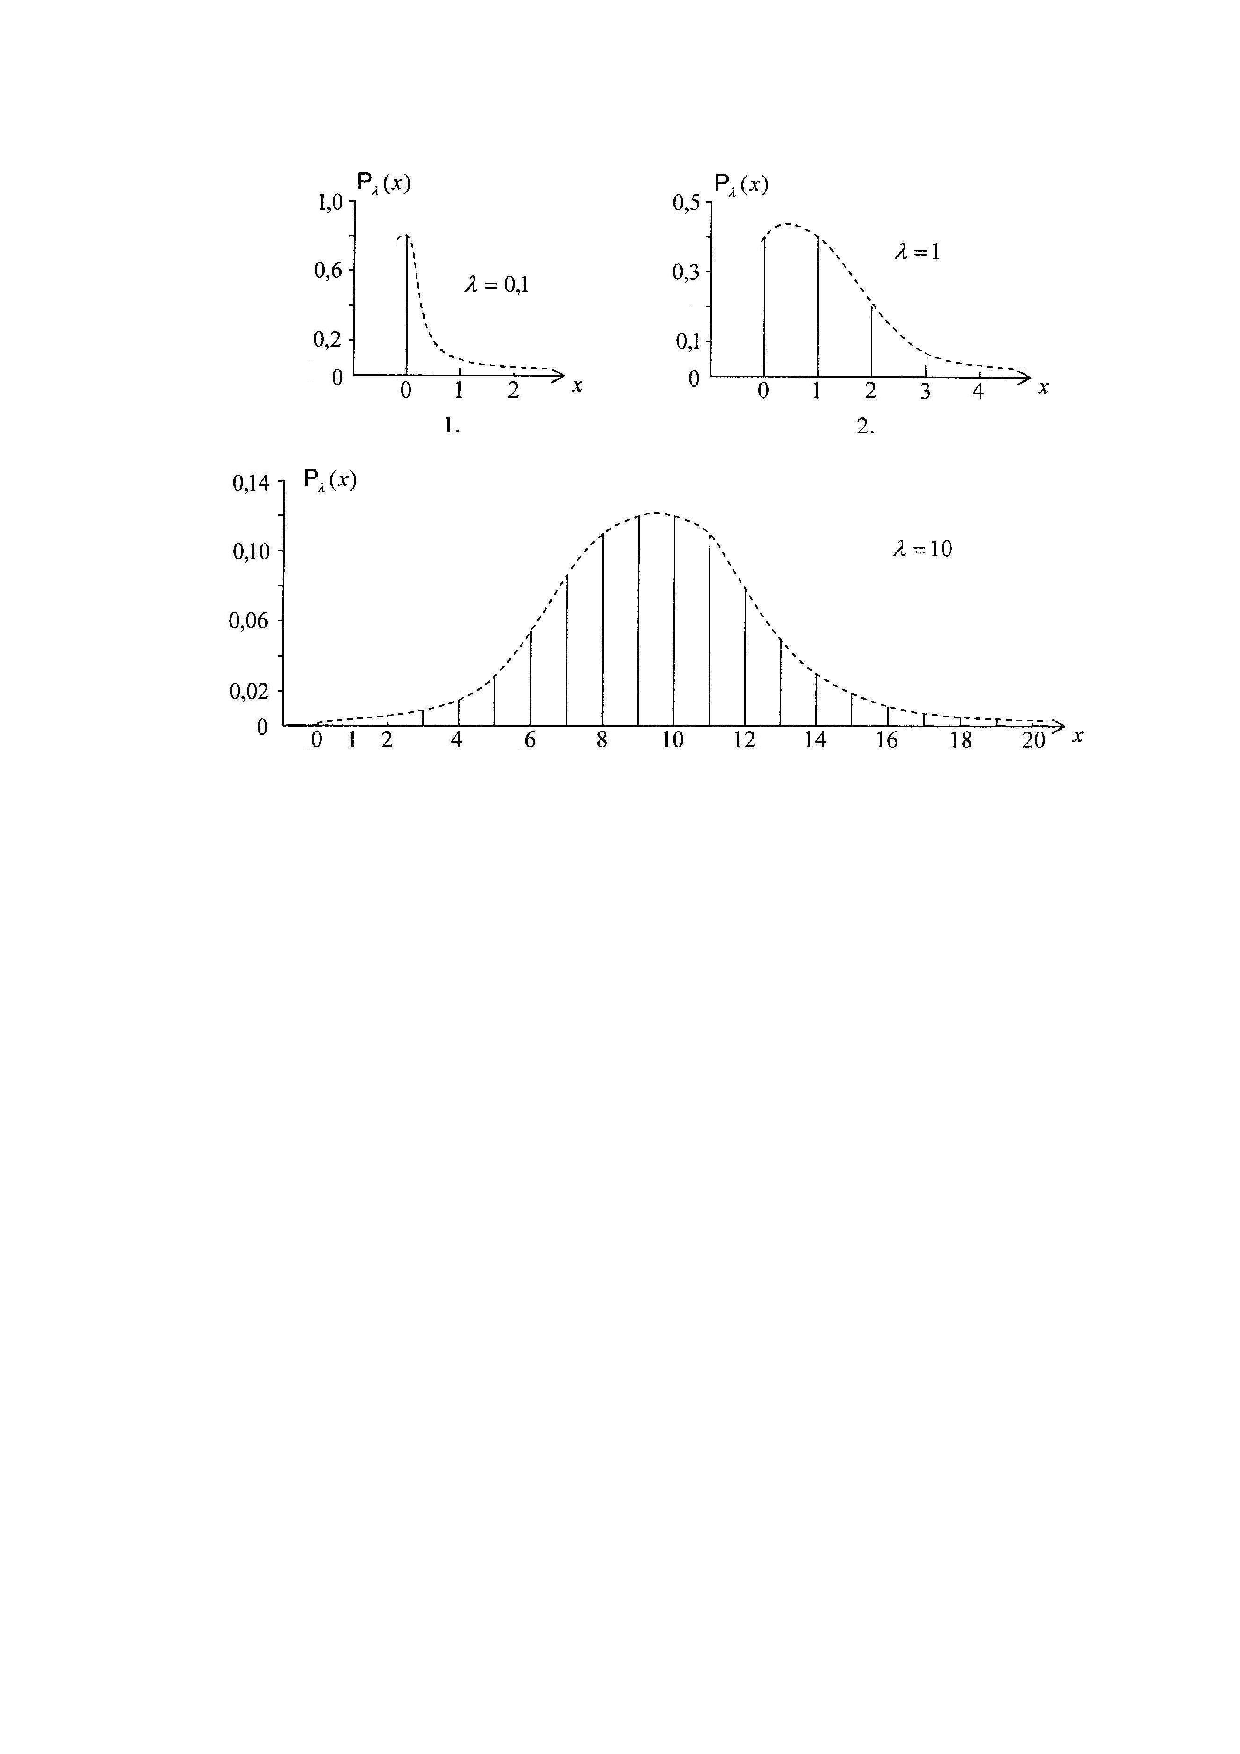
\includegraphics[]{pic/pic25}
	\caption{Распределение Пуассона}
	\label{fig25}
\end{figure} 
Рассмотрим бесконечную таблицу событий:
$$\begin{matrix} 
A_{11} &  &  &  &  \\
A_{21} & A_{22} &  &  &  \\
A_{31} & A_{32} & A_{33} &  &  \\
\ldots & \ldots & \ldots & \ldots &  \\
A_{n1} & A_{n2} & A_{n3} & \ldots & A_{nn}\\
\ldots & \ldots & \ldots & \ldots & \ldots\\   
\end{matrix}$$

где 1) в $n$-ой строке, $n = 1, 2, \ldots$ , стоят $n$ событий $A_{n1} , A_{n2} , A_{n3} , \ldots , A_{nn}$;
2) в каждой строке события попарно независимы;
3) каждое событие в $n$-ой строке происходит с одной и той же вероятностью $p_n$ , зависящей только от номера строки.
Обозначим через $\xi_n$ случайную величину, равную числу событий $A_{ni}$ , произошедших в $n$-ой строке. Ясно, что случайная величина $\xi_n$ принимает значения $k = 0, 1, 2, \ldots , n$ и имеет биномиальное распределение $k \to C_n^k p^k_n (1 − pn )^{n−k}.$

\begin{definition}
\label{def:23.3}
Говорят, что последовательность $p_1 , p_2 , \ldots ,
p_n , \ldots$ удовлетворяет закону малых чисел, если $\lim\limits_{n \to \infty} p_n = 0$ и существует предел
$$\lim\limits_{n \to \infty} np_n = \lambda, \quad \text{где} \quad  0 < \lambda < \infty.$$
\end{definition}

\begin{theorem}[Пуассона]
\label{th:23.4}
Если последовательность $\{ p_n\}_{n=1}^{\infty}$ удовлетворяет закону малых чисел, то для любого $k \geq 0$ имеет место равенство
$$\lim\limits_{n \to \infty} C_n^k p_n^k (1-p_n)^{n-k} = \frac{\lambda^k}{k!}e^{-\lambda}$$
\end{theorem}

\begin{proof}
Обозначим $\lambda_n = n \cdot p_n$ . Тогда

\begin{gather*}
	\P = (\xi_n = k) = C_n^k p_n^k (1 - p_n)^{n-k} =\\= 
	\frac{n(n-1) \ldots (n-k+1)}{k!}
	\left( \frac{\lambda_n}{n} \right)^k
	\left( 1 - \frac{\lambda_n}{n} \right)^{n-k} =\\=
	\frac{\lambda_n^k}{k!}\cdot
	\frac{n(n-1) \ldots (n-k+1)}{n^k}
	\left( 1 - \frac{\lambda_n}{n} \right)^{n}
	\left( 1 - \frac{\lambda_n}{n} \right)^{-k} =\\=
    \frac{\lambda^k_n}{k!} \left( 1 - \frac{1}{n} \right) \left( 1 - \frac{2}{n} \right) \ldots \left( 1 - \frac{k-1}{n} \right) \left( 1 - \frac{\lambda_n}{n} \right)^n \left( 1 - \frac{\lambda_n}{n} \right)^{-k}.
\end{gather*}

Отсюда переходя к пределу при $n \to \infty$ получим требуемый результат.
 \end{proof}

 \begin{zam}
 \label{zam:23.5}
Теорема Пуассона доставляет приближённую формулу

$$\P(\xi_n = k) = C^k_n p^k (1 − p_n )^{n−k} \approx \frac{(np)^k}{k!}e^{-np}$$

Заметим, что в примере \ref{ex:18.9}.2) мы вычислили математическое ожидание и дисперсию для биномиального распределения $\M \xi = np$ и $\D \xi = npq$.

Поэтому имеем

$$\P(\xi_n = k) \approx \frac{(\M \xi)^k}{k!}e^{-\M \xi}.$$

Параметр $\lambda = np$ является математическим ожиданием для распределения Пуассона. Таким образом, биномиальное распределение аппроксимируется распределением Пуассона так, что оба распределения имеют одно и то же математическое ожидание. На самом деле оба распределения имеют и достаточно близкие дисперсии. В области применения приближённой формулы вероятность $p$ должна быть мала, а значит $q = 1 − p \approx 1$, поэтому
$\D \xi = npq \approx np = \lambda$. 	
 \end{zam}

\textbf{Пример.} Вероятность попадания в цель при каждом выстреле равна 0,001. Найти вероятность попадания в цель двумя и более пулями, если число выстрелов равно 5 000.
Решение. Этот эксперимент реализует схему Бернулли, и использование точной формулы даёт значение искомой вероятности равное
\begin{gather}
	\label{pisk}
	\P(\xi_n \geq 2) = \sum\limits_{k=2}^{5000} \P(\xi_{5000} = k) =\\=\nonumber
	1 - \P(\xi_{5000} = 0) - \P(\xi_{5000} = 1) =\\=\nonumber
	1 − 0, 999^{5000} − 5000 \cdot 0, 001 \cdot 0, 999^{4999}.
\end{gather}
Воспользуемся теоремой Пуассона $\P(\xi_n = k) \approx \frac{(np)^k}{k!}e^{-np}$. 
Вычислим: $\lambda = np = 5000 \cdot 0, 001 = 5, \P(\xi_{5000} = 0) \approx e^{-5} , \P(\xi_{5000} = 1) \approx 5e^{−5}.$ 
Поэтому
$$\P_n (\xi \geq 2) = 1 − \P(\xi_{5000} = 0) − \P(\xi_{5000} = 1) \approx 1 − 6e^{−5} \approx 0, 9596.$$
Вычисление по точной формуле (\ref{pisk}) с точностью до четвёртого знака даёт ответ $P_n (\xi \geq 2) = 0, 9575$. Нетрудно подсчитать, что ошибка от применения приближённой формулы составляет меньше 0,25\%.

\subsection{Теорема Муавра} Эта предельная теорема обеспечивает приближённое вычисление вероятностей биномиального распределения,

$$\P(\xi_n = k) = C^k_n \cdot pk \cdot q^{n−k},$$

в случае, когда при $n \to \infty$ обе величины $k \to \infty$ и $n − k \to \infty$ так, что величина $x_k = \frac{k - np}{\sqrt{npq}}$ ограничена, т.е. существует $N > 0$, такое что $|x_k| < N$ для $k = 0, 1, 2, \ldots .$

\begin{theorem}[Локальная теорема Муавра\footnote{
\label{th:23.6}
Абрахам де Муавр (Abraham de Moivre, 1667 — 1754), английский математик французского происхождения. Основные труды по теории рядов, теории вероятностей, теории комплексных чисел.	
}]
Если вероятность $0 < p < 1$ постоянна, и величина $x_k = \frac{k - np}{\sqrt{npq}}$ ограничена, то справедлива формула
$$\lim\limits_{n \to \infty} 
\left[ C_n^k p^k q^{n-k} - \frac{1}{\sqrt{2\pi npq}} 
exp \left(-\frac{x_k^2}{2} \right) \right] = 0$$
(Без доказательства.)
\end{theorem}

\begin{zam}
\label{zam:23.7}
Локальная теорема Муавра доставляет приближённую формулу
$$\P(\xi_n = k) = C_n^k p^k q^{n-k} \approx \frac{1}{\sqrt{2\pi npq}} exp \left(-\frac{x_k^2}{2} \right)$$

Напомним, что в примере \ref{ex:18.9}.2) мы вычислили математическое ожидание и дисперсию для биномиального распределения $\M \xi = np$ и $\D \xi = npq$.
Поэтому имеем

\begin{gather*}
	x_k = \frac{k - np}{\sqrt{npq}}  = \frac{k - \M \xi}{\sqrt{\D \xi}} = \frac{K - \M \xi}{\sigma} \text{и}\\
	\P(\xi_n = k) \approx \frac{1}{\sigma \sqrt{2\pi}} exp \left(-\frac{(k - \M \xi)^2}{2 \sigma^2} \right) 
\end{gather*}

Последняя формула означает, что биномиальное распределение аппроксимировано нормальным, причём оба распределения имеют одинаковые математические ожидания и дисперсии.
\end{zam}

\textbf{Пример.}
Пусть надо вычислить $\P(\xi_n = k)$ при $n = 10 000, k = 40, p = 0, 005$. Сделаем подготовительные вычисления:

$$\sqrt{npq = \sqrt{10 000 \cdot 0,005 \cdot 0,995}} = \sqrt{49,75} \approx 7,05$$

$$\frac{k - np}{\sqrt{npq}} \approx -1,42.$$

По теореме Муавра имеем

$$\P(\xi_n = k) \approx \frac{1}{7,05\sqrt{2\pi}}\exp \left(-\frac{1,42^2}{2}\right).$$

Функция
$\phi(x) = \frac{1}{\sqrt{2\pi}}e^{-\frac{x^2}{2}}$
табулирована (см., например, Таблицу 23.8.8 в \cite{kk}), по таблице находим

$$\P(\xi_n = k) \approx \frac{0, 1456}{7,05} = 0,00206.$$

Заметим, что точное значение с точностью до третьего знака 
$\P(\xi_n = k) \approx 0,00197$. Полученная ошибка составляет 4,6 \%.


\begin{theorem}[Интегральная теорема Муавра(1730)--Лапласа\footnote{
\label{th:23.8}
Пьер-Симон Лаплас (Pierre-Simon Laplace, 1749 -- 1827), французский математик, астроном, физик и философ; известен работами по небесной механике, дифференциальным уравнениям, является одним
из создателей теории вероятностей. Заслуги Лапласа в чистой и прикладной математике и астрономии громадны: он усовершенствовал почти все разделы этих наук.
} (1812)]
Если случайная величина $\xi$ имеет биномиальное распределение $\P(\xi_n = k) = C^k_n p^k q^{n−k}$ , тогда для любых вещественных $k_1$ и $k_2$ имеет место равенство

$$\lim\limits_{n \to \infty} \P(k_1 \leq \xi_n \leq k_2 ) = \int\limits_x^y \frac{1}{\sqrt{2\pi}}e^{-\frac{t^2}{2}}dt,$$
где $x = \frac{k_1 - np}{\sqrt{npq}}$ и $y = \frac{k_2 - np}{\sqrt{npq}}.$
Теорему Муавра-Лапласа мы докажем в \S\ref{par:25} как частный случай центральной предельной теоремы.	
\end{theorem}.
% Рита

\section{Характеристические функции}
%!TEX root = ../var.tex

\begin{zam}
Решение многих задач теории вероятностей, особенно тех, которые связаны с суммированием независимых случайных величин, удаётся получить с помощью т.н. характеристических функций.
Связь между преобразованием Фурье и характеристической функцией можно описать следующим образом. Если обозначить преобразование Фурье через $\Phi$, то формулы прямого и обратного преобразования можно записать
следующим образом
\begin{gather*}
	\phi(t) = \Phi[f] = \frac{1}{\sqrt{2\pi}}\int\limits_{-\infty}^{\infty}e^{-ixt}f(x)dx, \\
%и
	f(x) = \Phi^{-1}[\phi] = \frac{1}{\sqrt{2\pi}} \int\limits_{-\infty}^{\infty}e^{itx}\phi(t)dt.   
\end{gather*}

Если $\xi$ — случайная величина, имеющая плотность $f_{\xi}(x)$, то в терминах преобразования Фурье её характеристическая функция есть
$$\Theta_{\xi} (t) = \sqrt{2\pi}\Phi^{-1}[f_{\xi}(x)] = \int\limits_{-\infty}^{\infty}e^{itx}dx$$
\end{zam}

\begin{definition}
	Пусть $f_{\xi}(x)$ -- плотность случайной величины $\xi$,
тогда функция
$$\Theta_{\xi}(t) = \M e^{it\xi} = \int\limits_{-\infty}^{\infty} e^{itx}f_{\xi}(x)dx$$

называется характеристической функцией случайной величины $\xi$.
\end{definition}

\begin{zam}
1) Пусть $\xi$ и $\eta$ -- вещесвенные случайные величины. Составим комплексную случайную величину $\xi + i\eta$. Мы распространяем действие знака математического ожидания $\M$ на любую комплексную случайную величину по свойству линейности:
$$\M(\xi + i\eta) = \M\xi + i \M\eta.$$

2) Зная характеристическую функцию $\Theta_{\xi} (t)$, можно однозначно восстановить функцию распределения, а также плотность вероятности или ряд распределения случайной величины $\xi$. Например, если модуль характеристической функции $\Theta_{\xi} (t)$ интегрируем на всей прямой, то плотность $f_{\xi}(x)$
случайной величины $\xi$ находится по формуле
$$f_{\xi}(x) =\frac{1}{2\pi}\int\limits_{-\infty}^{\infty}e^{itx}\Theta_{\xi} (t) dt.$$
\end{zam}

\textbf{Свойства характеристических функций}

\begin{theorem}
	Характеристическая функция $\Theta_{\xi} (t)$ любой случайной величины $\xi$ равномерно непрерывна. (Без доказательства.)
\end{theorem}

\begin{lemma}
\begin{enumerate}
	\item $\Theta_{\xi} (0) = 1$
	\item $|\Theta_{\xi} (t)| \leq 1 \text{для} −\infty < t < \infty$.
\end{enumerate}
\end{lemma}

\begin{proof}
\begin{enumerate}
	\item $\Theta_{\xi} (0) = \M e^0 = 1.$
	\item $|\Theta_{\xi} (t)| = |\M e^{it\xi} | \leq \M|e^{it\xi} | = \M 1 = 1.$
\end{enumerate}
\end{proof}

 \begin{lemma}
  	Если $\eta = a\xi + b$, где $a$ и $b$ — постоянные, то
$$\Theta_{\eta} (t) = \Theta_{\xi} (at) e^{ibt}.$$
  \end{lemma} 

  \begin{proof}
  	$\Theta_{\eta} (t) = \M e^{it\eta} = \M e^{it(a\xi+b)} = e^{ibt} \M e^{iat\xi} = e^{ibt} \Theta_{\xi} (at)$
  \end{proof}

\begin{lemma}
 Если $\xi_1$ и $\xi_2$ -- независимые случайные величины, то
$$\Theta_{\xi_1 +\xi_2} (t) = \Theta_{\xi_1} (t) \cdot \Theta_{\xi_2} (t).$$
 \end{lemma} 

\begin{proof}
	Т.к. $\xi_1$ и $\xi_2$ -- независимые величины, то $e^{it\xi_1}$ и $e^{it\xi_2}$ тоже независимы. Тогда

$$\Theta_{\xi_1 +\xi_2} (t) = \M e^{it(\xi_1 +\xi_2 )} = \M e^{it\xi_1} \cdot e^{it\xi_2} \stackrel{16.5.6)}{=}
= \M e^{it\xi_1} \cdot \M e^{it\xi_2} = \Theta_{\xi_1} (t) \cdot \Theta_{\xi_2} (t).$$
\end{proof}

\begin{consq}
Если $\xi_1 , \ldots , \xi_n$ — независимые случайные величины, то
$$\Theta_{\xi_1 + \ldots +\xi_2} (t) = \Theta_{\xi_1} (t) \cdot \ldots \cdot \Theta_{\xi_n} (t).$$
\end{consq}

\begin{lemma}
$\Theta_{\xi} (−t) = \overline{\Theta_{\xi}(t)}$, где черта означает комплексное сопряжение.
\end{lemma}

\begin{proof}
$\Theta_{\xi} (−t) = \M e^{−it\xi} = \M \overline{e^{it\xi}} = \overline{\M e^{it\xi}} = \overline{\Theta_{\xi} (t)}.$
\end{proof}

\begin{lemma}
Если $\xi$ — дискретная случайная величина, заданная рядом распределения (конечным или бесконечным)



\begin{center}
	\begin{tabular}{|c|c|c|c|c|}
		\hline
		$\xi$ & $x_1$ & $x_2$ & $\ldots$ & $x_k$ \\ \hline
		$P$  & $p_1$ & $p_2$  & $\ldots$ & $p_k$ \\ \hline
	\end{tabular}
\end{center}

то $\Theta_{\xi} (t) = \sum_k e^{itx_{k}} p_k$
\end{lemma}

\begin{proof}
Это утверждение непосредственно следует из теор. 17.4.1).
\end{proof}

\begin{lemma}
Пусть существует начальный момент $n$-го порядка,
$n = 1, 2, \ldots$, случайной величины $\xi$, т.е. $\M|\xi|^n < \infty$. Тогда её характеристическая функция $\Theta_{\xi} (t)$ является $n$ раз непрерывно дифференцируемой, и
её $n$-я производная в нуле равна
$$
\Theta_{\xi}^{(n)} (0) = i^n \M \xi^n $$
\end{lemma}

\begin{proof}
Заметим сначала, что т.к. существует начальный момент
$M\xi^n$ , то существуют все моменты $M\xi^k$ при $k < n$.

По лемме 24.5.2) имеем $|\Theta_{\xi} (t)| \leq 1$, поэтому интеграл в правой части 

$$\Theta_{\xi} (t) = \int\limits_{-\infty}^{\infty} e^{itx}f_{\xi}(x)dx$$

равномерно сходится по параметру $t$ и следовательно его можно дифференцировать по $t$:
\begin{gather*}
	\Theta_{\xi}' (t) = i \int\limits_{-\infty}^{\infty} xe^{itx} f_{\xi}(x)dx,\\
	\Theta_{\xi}'' (t) = i^2 \int\limits_{-\infty}^{\infty} x^2 e^{itx} f_{\xi}(x)dx,\\
	\ldots\ldots\ldots\ldots\ldots\ldots\ldots\\
	\Theta_{\xi}^(n) (t) = i^n \int\limits_{-\infty}^{\infty} x^n e^{itx} f_{\xi}(x)dx.
\end{gather*}

Подставляя в эти равенства $t = 0$, получим требуемый результат: 
$\Theta_{\xi}' (0) = i\M \xi, \Theta_{\xi}'' (0) = i^2 \M \xi^2 , \ldots , \Theta_{\xi}^{(n)} (0) = i^n \M \xi^n .$
\end{proof}

\begin{lemma}
Если существуют начальные моменты $\M \xi, \M \xi^2 , \ldots , \M \xi^n$ случайной величины $\xi$, т.е. $M |\xi|^n < \infty$, тогда в окрестности нуля её
характеристическая функция $\Theta_{\xi} (t)$ разлагается в ряд Тейлора\footnote{
Брук Тэйлор (Brook Taylor, 1685 — 1731), английский математик, именем которого назван ряд (опубликованный им в 1715—1717 гг.), однако этот ряд был известен и применялся ещё в XVII веке Грегори и Ньютоном.
}
$$\Theta_{\xi} (t) = 1 + \frac{i\M \xi}{1!}t + \frac{i^2 \M \xi^2}{2!}t^2 + \ldots + \frac{i^n \M \xi^n}{n!}t^n + \text{o}(t^n)$$
\end{lemma}

\begin{proof}
В стандартное разложение функции $\Theta_{\xi} (t)$ в ряд Тейлора
$$\Theta_{\xi} (t) = 1 + \frac{\Theta_{\xi}'(0)}{1!}t + \frac{\Theta_{\xi}''(0)}{2!}t^2 + \ldots + \frac{\Theta_{\xi}(n)(0)}{n!}t^n + \text{o}(t^n)$$ 

подставим выражения для $\Theta_{\xi}' (0), \Theta_{\xi}'' (0), \ldots , \Theta_{\xi} (0)$, доставляемые теор.
24.11, получим требуемый результат.
\end{proof}

% \textit{
В заключение параграфа сформулируем без доказательства теорему Леви, которая устанавливает <<непрерывное>> соответствие между слабо сходящимися последовательностями случайных величин и поточечно сходящимися последовательностями характеристических функций. <<Непрерывность>> этого соответствия состоит в том, что пределу при слабой сходимости соответствует предел при поточечной сходимости и наоборот.
% }

\begin{theorem}[Леви\footnote{Поль Пьер Леви (Paul Pierre Levy, 1886 — 1971), выдающийся французский математик, основные
труды по теории вероятностей, функциональному анализу, теории функций и механике.
} о непрерывном соответствии]
Последовательность случайных величин $\{\xi_n \}_{n=1}^{\infty}$ слабо сходится к случайной величине $\xi$
тогда и только тогда, когда последовательность их характеристических функций $\{\Theta_{\xi_n} (t)\}_{n=1}^{\infty}$ поточечно сходится к характеристической функции $\Theta_{\xi} (t)$.
\end{theorem}%Рита

\section{Вычисление характеристических
функций}
%!TEX root = ../var.tex

\begin{zam}
Решение многих задач теории вероятностей, особенно тех, которые связаны с суммированием независимых случайных величин, удаётся получить с помощью т.н. характеристических функций.
Связь между преобразованием Фурье и характеристической функцией можно описать следующим образом. Если обозначить преобразование Фурье через $\Phi$, то формулы прямого и обратного преобразования можно записать
следующим образом
\begin{equation*}
	\phi(t) = \Phi[f] = \frac{1}{\sqrt{2\pi}}\int\limits_{-\infty}^{\infty}e^{-ixt}f(x)dx,
%и
	f(x) = \Phi^{-1}[\phi] = \frac{1}{\sqrt{2\pi}} \int\limits_{-\infty}^{\infty}e^{itx}\phi(t)dt.   
\end{equation*}

Если $\xi$ — случайная величина, имеющая плотность $f_{\xi}(x)$, то в терминах преобразования Фурье её характеристическая функция есть
$$\Theta_{\xi} (t) = \sqrt{2\pi}\Phi^{-1}[f_{\xi}(x)] = \int\limits_{-\infty}^{\infty}e^{itx}dx$$
\end{zam}

\begin{definition}
	Пусть $f_{\xi}(x)$ -- плотность случайной величины $\xi$,
тогда функция
$$\Theta_{\xi}(t) = \M e^{it\xi} = \int\limits_{-\infty}^{\infty} e^{itx}f_{\xi}(x)dx$$

называется характеристической функцией случайной величины $\xi$.
\end{definition}

\begin{zam}
1) Пусть $\xi$ и $\eta$ -- вещесвенные случайные величины. Составим комплексную случайную величину $\xi + i\eta$. Мы распространяем действие знака математического ожидания $\M$ на любую комплексную случайную величину по свойству линейности:
$$\M(\xi + i\eta) = \M\xi + i \M\eta.$$

2) Зная характеристическую функцию $\Theta_{\xi} (t)$, можно однозначно восстановить функцию распределения, а также плотность вероятности или ряд распределения случайной величины $\xi$. Например, если модуль характеристической функции $\Theta_{\xi} (t)$ интегрируем на всей прямой, то плотность $f_{\xi}(x)$
случайной величины $\xi$ находится по формуле
$$f_{\xi}(x) =\frac{1}{2\pi}\int\limits_{-\infty}^{\infty}e^{itx}\Theta_{\xi} (t) dt.$$
\end{zam}

\textbf{Свойства характеристических функций}

\begin{theorem}
	Характеристическая функция $\Theta_{\xi} (t)$ любой случайной величины $\xi$ равномерно непрерывна. (Без доказательства.)
\end{theorem}

\begin{lemma}
\begin{enumerate}
	\item $\Theta_{\xi} (0) = 1$
	\item $|\Theta_{\xi} (t)| \leq 1 \text{для} −\infty < t < \infty$.
\end{enumerate}
\end{lemma}

\begin{proof}
\begin{enumerate}
	\item $\Theta_{\xi} (0) = \M e^0 = 1.$
	\item $|\Theta_{\xi} (t)| = |\M e^{it\xi} | \leq \M|e^{it\xi} | = \M 1 = 1.$
\end{enumerate}
\end{proof}

 \begin{lemma}
  	Если $\eta = a\xi + b$, где $a$ и $b$ — постоянные, то
$$\Theta_{\eta} (t) = \Theta_{\xi} (at) e^{ibt}.$$
  \end{lemma} 

  \begin{proof}
  	$\Theta_{\eta} (t) = \M e^{it\eta} = \M e^{it(a\xi+b)} = e^{ibt} \M e^{iat\xi} = e^{ibt} \Theta_{\xi} (at)$
  \end{proof}

\begin{lemma}
 Если $\xi_1$ и $\xi_2$ -- независимые случайные величины, то
$$\Theta_{\xi_1 +\xi_2} (t) = \Theta_{\xi_1} (t) \cdot \Theta_{\xi_2} (t).$$
 \end{lemma} 

\begin{proof}
	Т.к. $\xi_1$ и $\xi_2$ -- независимые величины, то $e^{it\xi_1}$ и $e^{it\xi_2}$ тоже независимы. Тогда

$$\Theta_{\xi_1 +\xi_2} (t) = \M e^{it(\xi_1 +\xi_2 )} = \M e^{it\xi_1} \cdot e^{it\xi_2} \stackrel{16.5.6)}{=}
= \M e^{it\xi_1} \cdot \M e^{it\xi_2} = \Theta_{\xi_1} (t) \cdot \Theta_{\xi_2} (t).$$
\end{proof}

\begin{consq}
Если $\xi_1 , \ldots , \xi_n$ — независимые случайные величины, то
$$\Theta_{\xi_1 + \ldots +\xi_2} (t) = \Theta_{\xi_1} (t) \cdot \ldots \cdot \Theta_{\xi_n} (t).$$
\end{consq}

\begin{lemma}
$\Theta_{\xi} (−t) = \overline{\Theta_{\xi}(t)}$, где черта означает комплексное сопряжение.
\end{lemma}

\begin{proof}
$\Theta_{\xi} (−t) = \M e^{−it\xi} = \M \overline{e^{it\xi}} = \overline{\M e^{it\xi}} = \overline{\Theta_{\xi} (t)}.$
\end{proof}

\begin{lemma}
Если $\xi$ — дискретная случайная величина, заданная рядом распределения (конечным или бесконечным)



\begin{center}
	\begin{tabular}{|c|c|c|c|c|}
		\hline
		$\xi$ & $x_1$ & $x_2$ & $\ldots$ & $x_k$ \\ \hline
		$P$  & $p_1$ & $p_2$  & $\ldots$ & $p_k$ \\ \hline
	\end{tabular}
\end{center}

то $\Theta_{\xi} (t) = \sum_k e^{itx_{k}} p_k$
\end{lemma}

\begin{proof}
Это утверждение непосредственно следует из теор. 17.4.1).
\end{proof}

\begin{lemma}
Пусть существует начальный момент $n$-го порядка,
$n = 1, 2, \ldots$, случайной величины $\xi$, т.е. $\M|\xi|^n < \infty$. Тогда её характеристическая функция $\Theta_{\xi} (t)$ является $n$ раз непрерывно дифференцируемой, и
её $n$-я производная в нуле равна
$$
\Theta_{\xi}^{(n)} (0) = i^n \M \xi^n $$
\end{lemma}

\begin{proof}
Заметим сначала, что т.к. существует начальный момент
$M\xi^n$ , то существуют все моменты $M\xi^k$ при $k < n$.

По лемме 24.5.2) имеем $|\Theta_{\xi} (t)| \leq 1$, поэтому интеграл в правой части 

$$\Theta_{\xi} (t) = \int\limits_{-\infty}^{\infty} e^{itx}f_{\xi}(x)dx$$

равномерно сходится по параметру $t$ и следовательно его можно дифференцировать по $t$:
\begin{gather*}
	\Theta_{\xi}' (t) = i \int\limits_{-\infty}^{\infty} xe^{itx} f_{\xi}(x)dx,\\
	\Theta_{\xi}'' (t) = i^2 \int\limits_{-\infty}^{\infty} x^2 e^{itx} f_{\xi}(x)dx,\\
	\ldots\ldots\ldots\ldots\ldots\ldots\ldots\\
	\Theta_{\xi}^(n) (t) = i^n \int\limits_{-\infty}^{\infty} x^n e^{itx} f_{\xi}(x)dx.
\end{gather*}

Подставляя в эти равенства $t = 0$, получим требуемый результат: 
$\Theta_{\xi}' (0) = i\M \xi, \Theta_{\xi}'' (0) = i^2 \M \xi^2 , \ldots , \Theta_{\xi}^{(n)} (0) = i^n \M \xi^n .$
\end{proof}

\begin{lemma}
Если существуют начальные моменты $\M \xi, \M \xi^2 , \ldots , \M \xi^n$ случайной величины $\xi$, т.е. $M |\xi|^n < \infty$, тогда в окрестности нуля её
характеристическая функция $\Theta_{\xi} (t)$ разлагается в ряд Тейлора\footnote{
Брук Тэйлор (Brook Taylor, 1685 — 1731), английский математик, именем которого назван ряд (опубликованный им в 1715—1717 гг.), однако этот ряд был известен и применялся ещё в XVII веке Грегори и Ньютоном.
}
$$\Theta_{\xi} (t) = 1 + \frac{i\M \xi}{1!}t + \frac{i^2 \M \xi^2}{2!}t^2 + \ldots + \frac{i^n \M \xi^n}{n!}t^n + \text{o}(t^n)$$
\end{lemma}

\begin{proof}
В стандартное разложение функции $\Theta_{\xi} (t)$ в ряд Тейлора
$$\Theta_{\xi} (t) = 1 + \frac{\Theta_{\xi}'(0)}{1!}t + \frac{\Theta_{\xi}''(0)}{2!}t^2 + \ldots + \frac{\Theta_{\xi}(n)(0)}{n!}t^n + \text{o}(t^n)$$ 

подставим выражения для $\Theta_{\xi}' (0), \Theta_{\xi}'' (0), \ldots , \Theta_{\xi} (0)$, доставляемые теор.
24.11, получим требуемый результат.
\end{proof}

% \textit{
В заключение параграфа сформулируем без доказательства теорему Леви, которая устанавливает <<непрерывное>> соответствие между слабо сходящимися последовательностями случайных величин и поточечно сходящимися последовательностями характеристических функций. <<Непрерывность>> этого соответствия состоит в том, что пределу при слабой сходимости соответствует предел при поточечной сходимости и наоборот.
% }

\begin{theorem}[Леви\footnote{Поль Пьер Леви (Paul Pierre Levy, 1886 — 1971), выдающийся французский математик, основные
труды по теории вероятностей, функциональному анализу, теории функций и механике.
} о непрерывном соответствии]
Последовательность случайных величин $\{\xi_n \}_{n=1}^{\infty}$ слабо сходится к случайной величине $\xi$
тогда и только тогда, когда последовательность их характеристических функций $\{\Theta_{\xi_n} (t)\}_{n=1}^{\infty}$ поточечно сходится к характеристической функции $\Theta_{\xi} (t)$.
\end{theorem}% Федя

\section{Центральная предельная теорема} 
%!TEX root = ../var.tex


\begin{zam}
\label{zam:26.1}
Центральные предельные теоремы (ЦПТ) в теории вероятностей -- это класс теорем, утверждающих, что сумма большого количества независимых случайных величин имеет распределение близкое к нормальному. 

Так как многие случайные явления в природе и социальном обществе являются суммами большого числа случайных факторов, то центральные предельные теоремы обосновывают фундаментальность нормального закона распределения. История получения ЦПТ растянулась на два века -- от первых работ Муавра 1730 г. до необходимых и достаточных условий, полученных в 30-х гг. XX века. 

Самый общий классический случай ЦПТ для неодинаково распределённых последовательностей случайных величин принадлежит А.М. Ляпунову\footnote{Александр Михайлович Ляпунов (1857 -- 1918), выдающийся русский математик, основные труды
по устойчивости динамических систем, теории потенциала и механике. Занятие теорией вероятностей было кратким эпизодом в его научной работе, тем не менее в этой области он добился фундаментальных результатов. Он доказал ЦПТ при весьма широких условиях методом, который и сейчас является одним
из основных в теории вероятностей.} (1901). Мы докажем ЦПТ в классической форме (теорема \ref{th:26.3}), а чтобы иметь представление о ЦПТ в форме Ляпунова (теорема \ref{th:26.5}) мы приведём её без доказательства. 
\end{zam}

\begin{zam}
\label{zam:26.2}
Вернёмся ещё раз к ЗБЧ в форме Хинчина. Пусть $$\xi_1 , \xi_2 , \ldots , \xi_n , \ldots$$ -- последовательность попарно независимых одинаково распределённых случайных величин, т.е. все имеющие математическое ожидание $\M\xi_1$ и дисперсию $\D\xi_1$. Обозначим $S_n=\sum\limits_{k=1}^n\xi_k$. 

Тогда по ЗБЧ в форме Хинчина среднее арифметическое $\frac{S_n}{n}$ сходится по вероятности к $\M\xi_1$, или, что то же самое, величина $\frac{S_n-n\M\xi_1}{n}$ сходится по вероятности к нулю. 

Запишем это утверждение с помощью неравенства Бьенеме – Чебышёва:
$$
\P\left( \left|\frac{S_n-n\M\xi_1}{n}\right| < \epsilon \right) \geq 1-\frac{\D\xi_1}{\epsilon^2}
$$

Т.к. вероятность не превосходит 1, то это неравенство можно переписать в виде
$$
1-\frac{\D\xi_1}{\epsilon^2} \geq \P\left( \left|\frac{S_n-n\M\xi_1}{n}\right| < \epsilon \right) \leq 1 
$$

Если теперь перейти к пределу при $n \to \infty$, то левая часть этого сквозного неравенства стремится к единице, и вероятность, стоящая в средней части, <<намертво>> впечатывается в единицу. В этом и состоит высший
смысл Закона Больших Чисел: при стремлении $n$ к бесконечности и для любого $\epsilon > 0$ неравенство  $\left|\frac{S_n-n\M\xi_1}{n}\right|  < \epsilon$ становится достоверным событием. 

Поэтому ЗБЧ есть строгое математическое выражение свойства
статистической устойчивости (см. определение \ref{def:4.4}). Заметим, что $\M\xi_1$ и $\D\xi_1$ являются константами, а $\epsilon > 0$ хотя и любое, но тоже постоянное число.

Идея как-то оторвать упомянутую вероятность от единицы заключается в следующем: а не слишком ли на большую степень числа n мы поделили в выражении $\frac{S_n-n\M\xi_1}{n}$?

Нельзя ли поделить на что-нибудь, растущее к бесконечности
медленнее чем $n$ так, чтобы последовательность событий
$\left\{\left|\frac{S_n-n\M\xi_1}{n^\alpha}\right|  < \epsilon\right\}$
при некотором $0 < \alpha < 1$ перестала бы сходиться к достоверному (и, само собой разумеется, не сходилась бы к невозможному событию)? 

Оказывается, если выбрать $\alpha = 1/2$, то при $n \to \infty$ последовательность случайных величин $\eta_n = \frac{S_n -n\M\xi}{\sqrt{n}}$ слабо сходится к случайной величине $\eta$, имеющей нормальное (!) распределение.
\end{zam}

\begin{theorem}[ЦПТ в классической форме]
\label{th:26.3}
Если случайные величины $$\xi_1 , \xi_2 , \ldots , \xi_n , \ldots$$ независимы, одинаково распределены и имеют конечные математическое ожидание $\M_{\xi} = a < \infty$ и дисперсию $\D_{\xi} = \sigma^2 < \infty$ и $\sigma \ne 0$, тогда последовательность случайных величин
$$
\eta_n =
\frac{
	\xi_1 + \ldots + \xi_n - na
}{\sigma\sqrt{ n}}
$$

слабо сходится к случайной величине, имеющей стандартное нормальное распределение, т.е.
$$
\lim\limits_{n\to\infty}
\P\left(
	\frac{
		\xi_1 + \ldots + \xi_n - na
	}{\sigma\sqrt{ n}}\leq x
\right)
=\frac{1}{\sqrt{2\pi}}\int\limits_{-\infty}^x e^{-u^2/2} du,
$$
или кратко
$$
\lim\limits_{n\to\infty}
\P\left(
	\eta_n \leq x
\right)
=\frac{1}{\sqrt{2\pi}}\int\limits_{-\infty}^x e^{-u^2/2} du,
$$
\end{theorem}
\begin{proof}
Для упрощения выкладок вместо $\xi_1 , \xi_2 , \ldots , \xi_n , \ldots$
введём стандартные случайные величины $\oxi_1 , \oxi_2 , \ldots , \oxi_n , \ldots$ по формулам
$$
\oxi_i=\frac{\xi_i-a}{\sigma}
$$

Легко видеть, что случайные величины $\oxi_i$ являются независимыми, одинаково распределёнными, имеют нулевое математическое ожидание и единичную дисперсию и следовательно имеют одинаковые характеристические функции. Обозначим их характеристические функции тем же символом как и для первой случайной величины $\theta_{\oxi_i}(t) = \theta_{\xi_1} (t)$. Используя лемму \ref{lemma:24.12}, разложим её в ряд Тейлора, содержащий три первых члена плюс остаточный член:
$$
\theta_{\oxi_i}(t)=1-\frac{1}{2}t^2+o(t^2),
$$

где мы учли, что $\M\oxi_1 = 0$ и $\M\oxi_1^2 = \D\oxi_1 + (\M\oxi_1)^2 = 1$.

Случайная величина $\eta_n$ может быть записана в виде
$$\eta_n =\frac{\oxi_1+\ldots+\oxi_n}{\sqrt{n}}=
\frac{\oxi_1}{\sqrt{n}}+\ldots+\frac{\oxi_n}{\sqrt{n}}
$$

Запишем и преобразуем её характеристическую функцию, получим
\begin{gather*}
\theta\eta_n (t) = \theta_{\frac{\oxi_1}{\sqrt{n}} + \ldots + \frac{\oxi_1}{\sqrt{n}}}(t)
\stackrel{24.8}{=}
\theta_{\frac{\oxi_1}{\sqrt{n}}}(t)\cdot\ldots\cdot \theta_{\frac{\oxi_1}{\sqrt{n}}}(t)
\stackrel{24.6}{=}\\=
\theta_{\oxi_1}\left(\frac{t}{\sqrt{n}}\right)
	\cdot\ldots\cdot
\theta_{\oxi_n}\left(\frac{t}{\sqrt{n}}\right)=
\left[
	\theta_{\oxi_1}\left(\frac{t}{\sqrt{n}}\right)
\right]^n=
\left[
	1-\frac{t^2}{2n}+o\left(\frac{t^2}{n}\right)
\right]^n
\end{gather*}

Т.к. по второму замечательному пределу имеем
$$
\lim\limits_{n\to\infty}
\left[
	1-\frac{t^2}{2n}+o\left(\frac{t^2}{n}\right)
\right]^n=e^{-t^2/2}
$$
то это означает, что последовательность характеристических функций
${\{\theta\eta_n (t)\}}_{n=1}^\infty$ поточечно сходится к характеристической функции 
${\theta\eta_n (t)}=e^{-t^2/2}$.

Из примера \ref{ex:25.5} эта функция является характеристической функцией стандартного нормального распределения с плотностью вероятности
$f_\eta (x) = \frac{1}{\sqrt{2\pi}}e^{-x^2/2}$. 

По теореме \ref{th:24.13} (Леви о непрерывном соответствии), последовательность случайных величин ${\{\eta_n \}}^\infty_{n=1}$ слабо сходится к случайной
величине $\eta$, а по определению \ref{def:21.9} слабой сходимости имеем
\begin{gather*}
\lim\limits_{n\to\infty} \P(\eta_n \leq x)
\stackrel{\ref{def:11.3}}{=}
\lim\limits_{n\to\infty} F_{\eta_n}(x)
\stackrel{\ref{def:21.9}}{=}
F_\eta(x)
\stackrel{\ref{def:12.1}}{=}
\frac{1}{\sqrt{2\pi}}\int\limits_{-\infty}^x e^{-u^2/2} du.
\end{gather*}
Что и требовалось доказать.
\end{proof}

\begin{consq}
\label{consq:26.4}
Если случайные величины $\xi_1 , \xi_2 , \ldots , \xi_n , \ldots$ независимы, одинаково распределены и имеют конечную ненулевую дисперсию и
$\eta_n =\frac{\xi_1+\xi_2+\ldots+\xi_n-na}{\sigma\sqrt{\pi}},$
то следующие утверждения эквивалентны ЦПТ в классической форме.

1) Для любых $x < y$ имеет место равенство:
$$
\lim\limits_{n\to\infty} \P(x<\eta_n<y)=
\frac{1}{\sqrt{2\pi}}\int\limits_{x}^y e^{-u^2/2} du.
$$

2) Для любых $x < y$ имеет место равенство:
$$
\lim\limits_{n\to\infty} \P(x \leq \eta_n \leq y)=
\frac{1}{\sqrt{2\pi}}\int\limits_x^y e^{-u^2/2} du.
$$

\end{consq}

\begin{theorem}[ЦПТ в форме Ляпунова]
\label{th:26.5}
Пусть случайные величины $$\xi_1 , \xi_2 , \ldots , \xi_n , \ldots$$ независимы и имеют конечные абсолютные начальные моменты 3-го порядка $(\M|\xi_n|^3 < \infty)$. Введём следующие обозначения:
$$
A_n=\sum\limits_{k=1}^n \M\xi_k,
\quad
B_n^2=\sum\limits_{k=1}^n \D\xi_k,
\quad
C_n^3=\sum\limits_{k=1}^n \M|\xi_k-\M\xi_k|^3.
$$

Если
$$
\lim\limits_{n\to\infty}\frac{C_n}{B_n}=0,
$$
тогда последовательность случайных величин
$$
\frac{\xi_1+\xi_2+\ldots+\xi_n-A_n}{B_n}
$$
слабо сходится к случайной величине, имеющей стандартное нормальное
распределение, т.е.
$$
\lim\limits_{n\to\infty} \P\left(\frac{\xi_1+\xi_2+\ldots+\xi_n-A_n}{B_n} \leq x\right)=
\frac{1}{\sqrt{2\pi}}\int\limits_{-\infty}^x e^{-u^2/2} du.
$$
\end{theorem}

В качестве следствия из ЦПТ докажем предельную теорему Муавра-Лапласа. Подобно ЗБЧ в форме Бернулли предельная теорема Муавра-Лапласа является утверждением только для схемы Бернулли. Напомним её формулировку.

\begin{theorem}[Интегральная теорема Муавра-Лапласа]
\label{th:26.6}
Если случайная величина $\eta_n$ имеет биномиальное распределение $\P(\eta_n = k) = C_n^k p^k q^{n-k}$, тогда для любых вещественных $k_1$ и $k_2$ имеет место равенство
$$
\lim\limits_{n\to\infty} \P\left(k_1\leq\eta_n\leq k_2\right)=
\frac{1}{\sqrt{2\pi}}\int\limits_{x}^{y} e^{-u^2/2} du,
$$
где $x=\frac{k_1-np}{\sqrt{npq}}$ и $y=\frac{k_2-np}{\sqrt{npq}}$.
\end{theorem}
\begin{proof}
Приведём обозначения теоремы Муавра-Лапласа в соответствие с обозначениями ЦПТ. Случайная величина $\xi$ есть число появлений события $A$ в результате $n$ испытаний в схеме Бернулли с вероятностью
$\P(A) = p$. 

Если обозначить через $\xi_i$ число (равное 0 или 1) появлений события $A$ в результате $i$-го испытания, где$ i = 1, \ldots , n,$ то случайную величину $\eta_n$ можно представить в виде суммы $\eta_n = \xi_1 + \ldots + \xi_n$ независимых, одинаково распределённых случайных величин, имеющих одинаковые конечные математические ожидания $\M_{\xi_i} = $p и дисперсии $\D_{\xi_i} = p(1 - p) = pq$. 

Тогда по пункту \ref{ex:18.9}.2) имеем $\M\eta_n = np$ и $\D\eta_n = npq$. 

Заметим, что неравенство $k_1\leq\eta_n\leq k_2$
эквивалентно неравенству
$$
\frac{k_1-np}{\sqrt{npq}}\leq
\frac{\eta_n-np}{\sqrt{npq}}\leq
\frac{k_2-np}{\sqrt{npq}}.
$$
По следствию \ref{consq:26.4}.2) получим требуемый результат.
\end{proof}

\begin{example}[Ср. пример \ref{ex:22.7}]
\label{ex:26.7}
Монету подбрасывают 10 000 раз. Найти вероятность того, что относительная частота выпадения герба отличается от классической вероятности $1/2$ не менее чем на $0,01$.


\textbf{Решение}. Другими словами, требуется найти $\P\left(\left|\frac{n(A)}{n}-\frac{1}{2}\right|\geq0,01\right)$, где $n = 10^4$ , $n(A) =
\sum\limits_{k=1}^n \xi_k$ -- число выпадений герба, а $\xi_k$ являются независимыми случайными величинами, имеющие одно и то же распределение
Бернулли с $p = \frac{1}{2}$, и равные единице, если выпал герб, и нулю -- в противном случае. 

Умножим обе части неравенства под знаком вероятности на $\sqrt{n} = 100$ и разделим на корень из дисперсии $\sqrt{\D\xi_1} = \sqrt{pq} = \frac{1}{2}$.
\begin{gather*}
	\P\left(
		\left|
			\frac{n(A)}{n}-p
		\right|\geq0,01
	\right)=
	1-\P\left(
		\left|
			\frac{n(A)-np}{n}
		\right|<0,01
	\right)=\\=
	1-\P\left(
		\frac{\sqrt{n}}{\sqrt{\D\xi_1}}
		\left|
			\frac{n(A)-np}{n}
		\right|<0,01\frac{\sqrt{n}}{\sqrt{\D\xi_1}}
	\right)=\\=
	1-\P\left(
		\left|
			\frac{n(A)-np}{\sqrt{npq}}
		\right|<2
	\right)=
	\frac{1}{\sqrt{2\pi}}\int\limits_{-2}^2 e^{-u^2/2} du=\\=
	1-2\Phi(2)\simeq 1 - 2 \cdot 0,47725 = 0,0455,
\end{gather*}
где значение $\Phi(2)$ интеграла вероятности взято из таблицы. Заметим,
что применение ЦПТ и предельной теоремы Муавра-Лапласа доставляет
лучшую оценку чем ЗБЧ в форме Бернулли (см. ответ в примере \ref{ex:22.7}).

\end{example}
% федя

\section{Сферическое, $\xi^2$-распределение и распределение Стьюдента} 
%!TEX root = ../var.tex

\subsection{Сферическое распределение}

\begin{definition}
Пусть случайные величины $\xi_1 , \ldots , \xi_n$ независимы и одинаково распределены по нормальному закону распределения
%
$$f_{\xi_i}(x_i) = \frac{1}{\sqrt{2\pi} \sigma} e^{-x^2_i/2\sigma^2},$$
%
то есть $a_i = 0$ и $\sigma_i = \sigma$ для всех 
%
$i = 1, \ldots , n.$ 
%
Тогда распределение случайного вектора $\xi = (\xi_1 , \ldots , \xi_n )$ называется нормальным сферическим распределением или проще сферическим распределением.
\end{definition}

\begin{lemma}
 Плотность вероятности сферического распределения есть
$$f_{\xi} (x_1 , \ldots , x_n ) = \frac{1}{(2\pi)^{n/2}\sigma^n} e^{-\frac{1}{2\sigma^2}(x_1^1 + \ldots + x^2_n)}$$
 \end{lemma} 

 \begin{proof}
 Это утверждение очевидно следует из 27.1 и 15.6.2).
 \end{proof}

\begin{zam}
Так как поверхности равной вероятности, то есть
$f_{\xi} (x_1 , \ldots , x_n ) = const$,
являются концентрическими $(n - 1)$ --мерными сферами $x^2_1 + \ldots + x^2_n = R^2$ 
с центром в начале координат, то сферическое распределение инвариантно относительно любого ортогонального преобразования
%
$A : \mathbb{R}^n \to \mathbb{R}^n$. 
%
То есть, если $\eta = A \cdot \xi$, то 
%
$f_{\eta}(x_1 , \ldots , x_n) = f_{\xi} (x_1 , \ldots , x_n )$,
%
где через $A$ обозначена ортогональная матрица.

Положим в сферическом распределении $\sigma = 1$, получим плотность вероятности

$$f_{\xi}(x_1, \ldots, x_n) = \frac{1}{(2\pi)^{n/2}}e^{-\frac{1}{2}(x_1^2 + \ldots + x_n^2)} $$

и назовём её плотностью вероятности стандартного сферического распределения.
\end{zam}

\subsection{$\chi$-- и $\chi^2$-- распределения}

\begin{definition}
Пусть случайные величины $\xi_1 , \ldots , \xi_n$ независимы и одинаково распределены по стандартному нормальному закону распределения. Случайные величины

$$\chi = \sqrt{\xi_1^2 +\ldots + \xi_n^2 }$$

и

$$\chi^2 = \xi_1^2 + \ldots + \xi_n^2$$

называются соответственно $\chi-$ и $\chi^2$ -распределениями с $n$ степенями свободы.

Наша ближайшая задача найти их плотности вероятности $f_{\chi} (x)$ и $f_{\chi^2} (x)$.
\end{definition}

\begin{figure}[H]
	\centering
	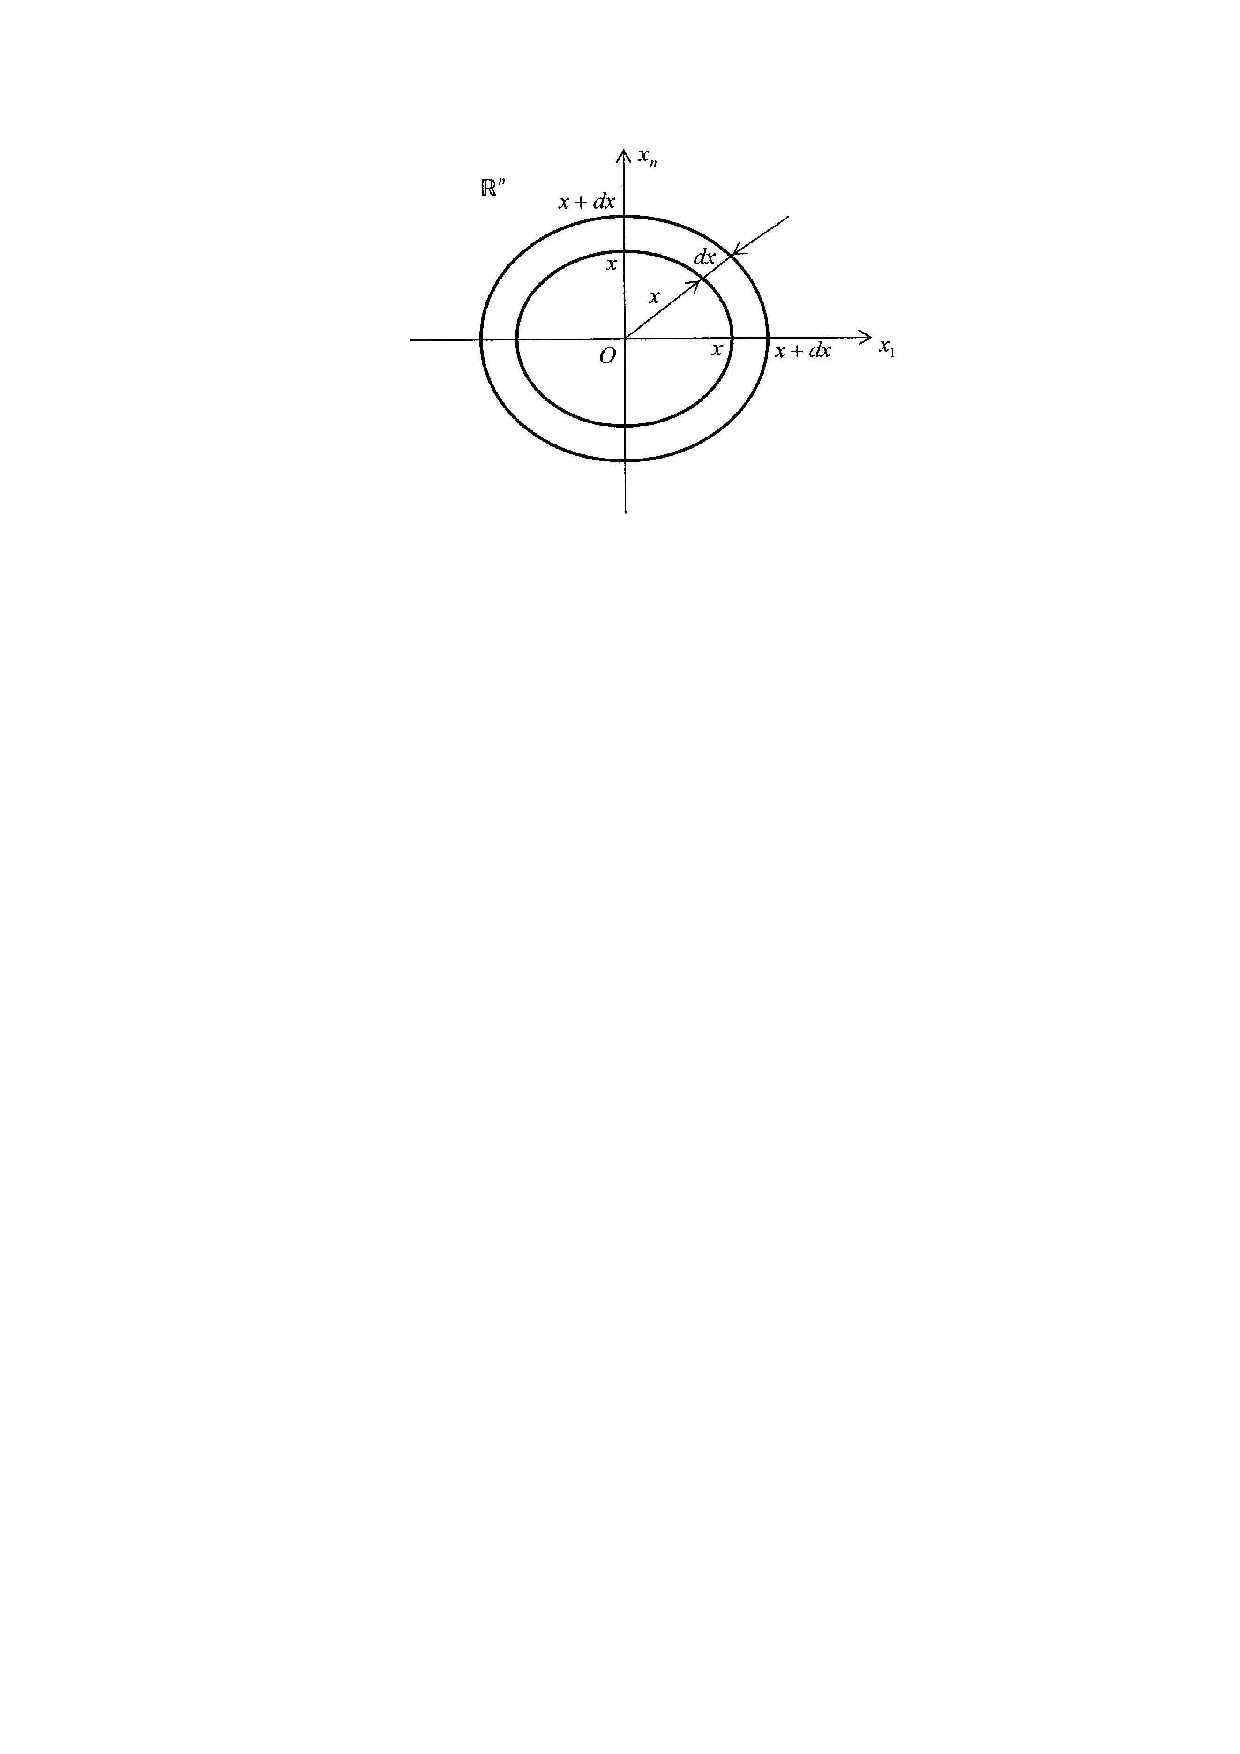
\includegraphics[]{pic/pic26}
	\caption{К вычислению плотности $\chi$-распределения}
	\label{fig26}
\end{figure}

\begin{theorem}
Плотность вероятности $\chi$-распределения задаётся по
формуле
$$f_{\chi} (x) = \frac{x^{n-1}}{2^{\frac{n}{2}-1}\Gamma(\frac{n}{2})} e^{-\frac{1}{2}x^2}, x\geqslant 0$$
где $\Gamma (x)$— гамма-функция.
\end{theorem}

\begin{proof}
Вероятность события $\{x < \chi < x + dx \}$ можно вычислить, интегрируя плотность вероятности $f_{\xi} (x_1 , \ldots , x_n )$ стандартного сферического распределения по $n$-мерному сферическому слою радиуса $x$ и толщины $dx$
(см. рис. 26).

$$ P(x < \chi < x + dx) = \dotsint\limits_{x<\sqrt{x_1^2 + \ldots + x_n^2}<x + dx} f_{\xi} (x_1 , \ldots , x_n ) dx_1 \ldots dx_n .$$

Откуда получаем

\begin{gather*}
f_{\xi} (x) = 
\frac{\P(x < \chi < x+dx)}{dx} = 
%
\dotsint\limits_{\sqrt{x_1^2 + \ldots + x_n^2} = x} 
f_{\xi}(x_1, \ldots, x_n)dx_1 \ldots dx_n = \\=
%
\frac{1}{(2\pi)^{n/2}} 
\dotsint\limits_{\sqrt{x_1^2 + \ldots + x_n^2} = x} e^{-\frac{1}{2}(x_1^2 + \ldots + x_n^2)}dx_1 \ldots dx_n = \\=
%
\frac{1}{(2\pi)^{n/2}}e^{-\frac{1}{2}x^2} 
\dotsint\limits_{\sqrt{x_1^2 + \ldots + x_n^2} = x} dx_1 \ldots dx_n = Cx^{n-1}e^{-\frac{1}{2}x^2}
\end{gather*}

где последнее равенство справедливо потому, что площадь $(n - 1)$-мерной сферы радиуса $x$ пропорциональна $x^{n-1}$ . Чтобы найти константу $C$, воспользуемся свойством плотности $\int\limits_0^{\infty} f_{\chi} (x) dx = 1$, откуда получаем

$$C\int\limits_0^{\infty}x^{n-1}e^{-\frac{1}{2}x^2}dx = 2^{\frac{n}{2}-1} \Gamma(\frac{n}{2})C = 1$$

откуда и следует требуемый результат.
\end{proof}

\begin{theorem}
Плотность $f_{\chi^2} (x)$ случайной величины $\chi^2$ есть

$$ f_{\chi^2} (x) = \frac{x^{\frac{n}{2}-1}}{2^{\frac{n}{2}} \Gamma (\frac{n}{2})}e^{-\frac{x}{2}}, \quad x \geq 0$$ 
\end{theorem}

\begin{proof}
Ясно, что случайные величины $\chi$ и $\chi^2$ связаны функцией $g(x) = x^2$ . Поэтому по теор. 14.2, находим, что
$$f_{\chi^2} (x) = |(g^{-1}(x))'| \cdot f_{\chi}(g^{-1}(x)) = \frac{1}{2\sqrt{x}}f_{\chi}(\sqrt{x}) = \frac{x^{\frac{n}{2}-1}}{2^{\frac{n}{2}} \Gamma(\frac{n}{2})} e^{-\frac{x}{2}}, \quad x \geq 0$$ 
 \end{proof} 

 \begin{zam}
Заметим, что $\chi^2$ -распределение с двумя степенями
свободы $(n = 2)$ является показательным распределением 12.7 с параметром $\lambda = 1/2$ и с плотностью вероятности $\frac{1}{2}e^{-\frac{x}{2}}, x \geq 0$. А $\chi$-распределение с тремя степенями свободы $(n = 3)$ называется распределением Максвелла и описывает в кинетической теории газов распределение модуля скорости
частиц в состоянии термодинамического равновесия.
 \end{zam}

\subsection{О распределении Стьюдента}

\begin{zam}
Этот пункт имеет информативный характер. Распределение Стьюдента\footnote{Стьюдент — псевдоним английского химика и статистика Вильяма Госсета (William Sealy Gosset, 1876
— 1937). По окончании университета был (с 1899) младшим управляющим пивоваренной компании в Дублине. В то время в совете директоров компании уже понимали важность методов
теории вероятностей и статистики для массового производства и направили Госсета на стажировку в
Лондонский университет для изучения статистики. Вскоре Госсет получил теоретические результаты в
статистике, которые оказались важными для пивоварения и которые он хотел опубликовать. В компании
не возражали против его публикаций, однако совет директоров хотел, чтобы конкуренты как можно
дольше не знали о применении статистики на пивоварне. Это объясняет появление псевдонима Стьюдент.} часто возникает в прикладных задачах математической статистики. Пусть случайные величины $\xi_0 , \xi_1 , \ldots , \xi_n$ независимы и одинаково распределены по стандартному нормальному закону распределения

$$f_{\xi_i} (x_i) = \frac{1}{\sqrt{2\pi}}e^{{-x^2_i/2}}$$

для всех $i = 0, 1, \ldots , n$. Тогда случайная величина

$$\tau_n = \frac{\xi_0}{\sqrt{\frac{1}{n}(\xi_1^2 + \ldots + \xi_n^2)}}$$

называется отношением Стьюдента, её распределение называется распределением Стьюдента с $n$ степенями свободы. Формула плотности вероятности $\tau_n$ имеет вид

$$f_{\tau_n}(x) = \frac{\Gamma(\frac{n+1}{2})}{\sqrt{n\pi}\Gamma(\frac{n}{2})} \left(1 + \frac{x^2}{n} \right)^{-\frac{n+1}{2}}, \quad -\infty < x < \infty$$
\end{zam} 

\begin{zam}
Легко проверить, что последовательность отношений Стьюдента $\{ \tau_n\}^{\infty}_{n=1}$ слабо сходится к стандартному нормальному распределению, то есть

$$\lim\limits_{n \to \infty} f_{\tau_n}(x) = \frac{1}{\sqrt{2\pi}}e^{-\frac{x^2}{2}}$$
\end{zam} % Рита

\section{Цепи Маркова} 
%!TEX root = ../var.tex

Непосредственным обобщением схемы независимых испытаний (см. определение 
\ref{lemma:9.3}) является схема цепей Маркова.

\begin{definition}
\label{def:28.1}
Пусть эксперимент состоит в том, что
\begin{enumerate}
	\item проводят последовательность испытаний с номерами $s = 1, 2, \ldots$ ;
	\item в каждом испытании появляется одно из $k$ несовместных событий
	$$A_1 , A_2 , \ldots , A_k,$$ при этом то, что в $s$-ом испытании произошло событие $A_i$ , будем обозначать $A^s_i$ ;
	\item вероятность появления события $A^{s+1}_j$ (то есть $j$-го события в $(s+1)$-ом испытании) зависит только от того, какое событие произошло в предыдущем $s$-ом испытании и не зависит от того, какие события произошли в испытаниях с номерами $s − 1, s − 2, \ldots $.
Тогда такая последовательность событий называется (простой) цепью Маркова.
\end{enumerate}

\end{definition}

\textbf{Пример.} Согласно предложенной Н. Бором\footnote{Нильс Хенрик Давид Бор (Niels Henrik David Bohr, 1865 — 1962), датский физик, один из создателей
квантовой физики. Создал первую квантовую модель атома, участвовал в разработке основ квантовой
механики, теории атомного ядра, ядерных реакций и взаимодействия элементарных частиц со средой.
} модели атома водорода электрон может находится только на одной из допустимых орбит. Обозначим через  $A_i$ событие, состоящее в том, что электрон находится на
$i$-ой орбите. Эти события Бор назвал стационарными состояниями атома. Вероятность перехода электрона с $i$-ой на $j$-ю орбиту зависит только от $i$ и $j$, потому что разность $j − i$ зависит от количества испускаемой
или поглощаемой атомом энергии и не зависит от того, на каких орбитах находился электрон в прошлом. Этот пример доставляет цепь Маркова теоретически с бесконечным числом состояний атома.

Теория цепей Маркова довольно обширна, поэтому мы ограничимся изучением так называемых однородных цепей Маркова.

Рассмотрим условную вероятность $\P(A^{s+1}_j|A^s_i)$,т.е. вероятность появления события $A_j^{s+1}$ при условии, что событие $A^s_i$ произошло.

\begin{definition}
\label{def:28.2}
Цепь Маркова называется однородной, если условная вероятность $\P(A^{s+1}_j|A^s_i)$ не зависит от номера $s$.

При этом вероятность $\P(A^{s+1}_j|A^s_i)$ называется вероятностью перехода от события $A^s_i$ к событию $A^{s+1}_j$ и обозначается
$$p_{ij} = \P(A^{s+1}_j|A^s_i)$$
\end{definition}

\begin{zam}
\label{zam:28.3}
Ясно, что

1) $0 \leq p_{ij} \leq 1$ и

2) $p_{i1} + p_{i2} + \ldots + p_{ik} = 1$ для всех $i = 1, 2, \ldots , k.$
\end{zam}

\begin{definition}
\label{def:28.4}
Полная информация о вероятностях перехода в цепи Маркова содержится в таблице

$$\pi_1 = \begin{pmatrix} 
p_{11} & p_{12} & \ldots & p_{1k}\\
p_{21} & p_{22} & \ldots & p_{2k}\\
\ldots & \ldots & \ldots & \ldots\\
p_{k1} & p_{k2} & \ldots & p_{kk}\\
\end{pmatrix}
$$
которая называется матрицей перехода.
\end{definition}

\begin{zam}
\label{zam:28.5}
Главной задачей теории цепей Маркова является нахождение вероятности перехода от события $A^s_i$ к событию $A^{s+n}_
j$ , произошедшему через $n$ испытаний. Обозначим эту вероятность
$$p_{ij}(n) = \P(A^{s+n}_j|A^s_i),$$
а искомую матрицу перехода через n испытаний через
$$\pi_n = 
\begin{pmatrix} 
p_{11}(n) & p_{12}(n) & \ldots & p_{1k}(n)\\
p_{21}(n) & p_{22}(n) & \ldots & p_{2k}(n)\\
\ldots & \ldots & \ldots & \ldots\\
p_{k1}(n) & p_{k2}(n) & \ldots & p_{kk}(n)$$
\end{pmatrix}
$$
\end{zam} 

\begin{theorem}
\label{th:28.6}
	Если $0 < m < n$, то $\pi_n = \pi_m \cdot \pi_{n−m} .$
\end{theorem}

\begin{proof}
Рассмотрим какое-нибудь промежуточное испытание с номером $s + m$, то есть $s < s + m < s + n$. Пусть в этом испытании появится какое-то событие $A^{s+m}_r$, где $1 \leq r \leq k$. В наших обозначениях вероятность перехода от события $A^s_i$ к событию $A^{s+m}_r$ равна
$$\P(A^{s+m}_r|A^s_i) = p_{ir}(m),$$
а вероятность перехода от события $A^{s+m}_r$ к событию $A^{s+n}_j$ равна
$$\P(A^{s+n}_j|A^{s+m}_r) = p_{ir}(n-m)$$
По формуле полной вероятности \ref{th:7.2} имеем
$$p_{ij}(n) = \sum\limits_{r+1}^k p_{ir}(m) \cdot p_{rj}(n-m).$$

Последняя формула в точности совпадает с формулой произведения матриц, поэтому получаем $\pi_n = \pi_m \cdot \pi_{n−m} .$
\end{proof} 

\begin{theorem}
\label{th:28.7}
 	Для любого $n \geq 1$, имеет место формула $\pi_n = \pi_1^n$ .
 \end{theorem} 

\begin{proof}
Доказательство проведём методом математической индукции.
\begin{enumerate}
	\item Проверяем тождество при $n = 1$: $\pi_1 = \pi^1_1 = \pi_1$.
	\item Пусть при $n = q$ выполнено тождество $\pi_q = \pi_1^q .$
	\item По теор. 28.6 имеем $\pi_{q+1} = \pi_1 \cdot \pi_q = \pi_1 \cdot \pi_1^q = \pi_1^{q+1}$.
\end{enumerate}
Что и требовалось доказать.
\end{proof}% Рита

\newpage
\begin{thebibliography}{12} 
\bibitem{gn}
	Гнеденко Б.В. Курс теории вероятностей. --М.:Наука, 1988.
\bibitem{ch}
	Чистяков В.П. Курс теории вероятностей. –М.:Наука, 1996.
\bibitem{}
	Боровков А.А. Теория вероятностей. – М.:Эдиториал УРСС, 1999.
\bibitem{baa}
	Севастьянов Б.А. Курс теории вероятностей и математической статистики. –М.:Наука, 1982.
\bibitem{dgb}
	Двайт Г.Б. Таблицы интегралов и другие математические формулы.
	9. –СПб.:Лань, 2005.
\bibitem{kk}
	Корн Г., Корн Т. Справочник по математике для научных работников и инженеров. М.: Наука, 1968.
\bibitem{dub}
	Задачи по теории вероятностей (Сост. А.А. Дубков, А.Т. Гаврилин) Метод. разработка для студентов РФ ф-та ННГУ. –Н.Новгород: ННГУ, 1999. %Диск I://students/libr/probabilitytheory/met-99/.pdf
\bibitem{sbz}
	Сборник задач по теории вероятностей, математической статистике и теории случайных функций (под редакцией А.А. Свешникова). М.: Наука, 1970.
\bibitem{kf}
	Коваленко И.Н., Филиппова А.А. Теории вероятностей и математической статистики. –М.: Высшая школа, 1992.
\bibitem{vec}
	Вентцель Е.С. Теория Вероятностей. –М.: Высшая школа, 1998.
\bibitem{giis}
	Гихман И.И., Скороход А.В., Ядренко М.И. Теории вероятностей и математической статистики. –Киев: Высшая школа, 1988.
\bibitem{agi}
	Агапов Г.И. Задачник по теории вероятностей –М.: Высшая школа,1996.
\bibitem{chni}
	Чернова Н.И. Теория вероятностей: Учеб. пособие/Новосиб. гос ун-т. Новосибирск, 2007. 160 с.
\end{thebibliography}

\end{document}